\documentclass[a4paper,12pt, oneside]{book}

% \usepackage{fullpage}
\usepackage[italian]{babel}
\usepackage[utf8]{inputenc}
\usepackage{amssymb}
\usepackage{amsthm}
\usepackage{graphics}
\usepackage{amsfonts}
\usepackage{listings}
\usepackage{amsmath}
\usepackage{amstext}
\usepackage{engrec}
\usepackage{rotating}
\usepackage{verbatim}
\usepackage{multicol}
\usepackage[safe,extra]{tipa}
% \usepackage{showkeys}
\usepackage{multirow}
\usepackage{hyperref}
\usepackage{microtype}
\usepackage{fontspec}
\usepackage{scrextend}
\usepackage{enumerate}
\usepackage{tabulary}
\usepackage{physics}
\usepackage{braket}
\usepackage{mhchem}
\usepackage{marginnote}
\usepackage{pgfplots}
\usepackage{cancel}
\usepackage{polynom}
\usepackage{booktabs}
\usepackage{enumitem}
\usepackage{framed}
\usepackage{pdfpages}
\usepackage{pgfplots}
\usepackage{algorithm}
% \usepackage{algpseudocode}
\usepackage[cache=false]{minted}
\usepackage{mathtools}
\usepackage[noend]{algpseudocode}
\newcommand*{\bfrac}[2]{\genfrac{}{}{0pt}{}{#1}{#2}}

\usepackage{tikz}\usetikzlibrary{er}\tikzset{multi  attribute /.style={attribute
    ,double  distance =1.5pt}}\tikzset{derived  attribute /.style={attribute
    ,dashed}}\tikzset{total /.style={double  distance =1.5pt}}\tikzset{every
  entity /.style={draw=orange , fill=orange!20}}\tikzset{every  attribute
  /.style={draw=MediumPurple1, fill=MediumPurple1!20}}\tikzset{every
  relationship /.style={draw=Chartreuse2,
    fill=Chartreuse2!20}}\newcommand{\key}[1]{\underline{#1}}
\usetikzlibrary{arrows.meta}
\usetikzlibrary{decorations.markings}
\usetikzlibrary{arrows,shapes,backgrounds,petri}
\tikzset{
  place/.style={
    circle,
    thick,
    draw=black,
    minimum size=6mm,
  },
  transition/.style={
    rectangle,
    thick,
    fill=black,
    minimum width=8mm,
    inner ysep=2pt
  },
  transitionv/.style={
    rectangle,
    thick,
    fill=black,
    minimum height=8mm,
    inner xsep=2pt
  }
} 
\usetikzlibrary{automata,positioning,chains,fit,shapes}
\usetikzlibrary{circuits.logic.US}
\usetikzlibrary{positioning}
\usepackage{fancyhdr}
\pagestyle{fancy}
\fancyhead[LE,RO]{\slshape \rightmark}
\fancyhead[LO,RE]{\slshape \leftmark}
\fancyfoot[C]{\thepage}
\usepackage[usenames,dvipsnames]{pstricks}
\usepackage{epsfig}
\usepackage{pst-grad} % For gradients
\usepackage{pst-plot} % For axes
\usepackage[space]{grffile} % For spaces in paths
\usepackage{etoolbox} % For spaces in paths
\makeatletter % For spaces in paths
\patchcmd\Gread@eps{\@inputcheck#1 }{\@inputcheck"#1"\relax}{}{}
\makeatother
\usepackage{lipsum}
\DeclareSymbolFont{symbolsC}{U}{txsyc}{m}{n}
\DeclareMathSymbol{\strictif}{\mathrel}{symbolsC}{74}
\title{Computational Systems Biology}
\author{UniShare\\\\Davide Cozzi\\\href{https://t.me/dlcgold}{@dlcgold}}
\date{}

\pgfplotsset{compat=1.13}
\begin{document}
\maketitle

\definecolor{shadecolor}{gray}{0.80}
\setlist{leftmargin = 2cm}
\newtheorem{teorema}{Teorema}
\newtheorem{definizione}{Definizione}
\newtheorem{esempio}{Esempio}
\newtheorem{corollario}{Corollario}
\newtheorem{lemma}{Lemma}
\newtheorem{osservazione}{Osservazione}
\newtheorem{nota}{Nota}
\newtheorem{esercizio}{Esercizio}
\algdef{SE}[DOWHILE]{Do}{doWhile}{\algorithmicdo}[1]{\algorithmicwhile\ #1}
\tableofcontents
\renewcommand{\chaptermark}[1]{%
  \markboth{\chaptername
    \ \thechapter.\ #1}{}}
\renewcommand{\sectionmark}[1]{\markright{\thesection.\ #1}}
\newcommand{\floor}[1]{\lfloor #1 \rfloor}
\newcommand{\MYhref}[3][blue]{\href{#2}{\color{#1}{#3}}}%
\chapter{Introduzione}
\textbf{Questi appunti sono presi a lezione. Per quanto sia stata fatta
  una revisione è altamente probabile (praticamente certo) che possano
  contenere errori, sia di stampa che di vero e proprio contenuto. Per
  eventuali proposte di correzione effettuare una pull request. Link: }
\url{https://github.com/dlcgold/Appunti}.\\
\chapter{Introduzione alla Systems Biology}
Per descrivere sistemi biologici complessi si hanno vari tipi di modelli.\\
Kitano (il ``padre'' di quest'ambito), nel 2002, disse che per capire i sistemi
biologici complessi bisogna integrare risultati sperimentali e metodi
computazionali, ottenendo quindi la 
vera e propria \textbf{Systems Biology}. Tramite l'interazione di vari
componenti si ottengono tali sistemi. Disse infatti:
\begin{center}
  \textit{To understand complex biological systems requires the integration of
    experimental and computational research — in other words a systems biology
    approach.} 
\end{center}
Weston, nel 2004, ha aggiunto l'importanza dello studio delle interazioni e
delle regolazioni tra i vari componenti del sistema, studiando le risposte alla
genetica o alle perturbazioni ambientali, al fine di capire nuove proprietà del
sistema. Infatti disse:
\begin{center}
  \textit{Systems biology is the analysis of the relationships among the
    elements in a system in response to genetic or environmental perturbations,
    with the goal of understanding the system or the emergent properties of the
    system} 
\end{center}
Ideker (altro ``padre'' di quest'ambito), già nel 2001, aveva definito la System
Biology come l'integrazione dei 
dati sperimentali con i modelli matematici che descrivono componenti e
interazioni, al fine di simulare il comportamento complessivo ``in silico''. Nel
dettaglio, citandolo:
\begin{center}
  \textit{Systems biology studies biological systems by systematically
    perturbing them (biologically, genetically, or chemically); monitoring the
    gene, protein, and informational pathway responses; integrating these data;
    and ultimately, formulating mathematical models that describe the structure
    of the system and its response to individual perturbations} 
\end{center}
Ai metodi standard della biologia quindi si aggiungono le teorie
informatiche, quelle matematiche, quelle fisiche, quelle chimiche, quelle
ingegneristiche. A partire dal fenomeno biologico quindi si effettuando
esperimenti, ottenendo dei dati sperimentali relativi alle funzioni, alle
strutture e alle interazioni delle varie componenti biologiche. A partire da
questi dati si costruisce un \textbf{modello matematico} che porterà alla
produzione 
di \textit{ipotesi} a partire da esso. Inoltre l'insieme di ipotesi produrrà
nuovi dati che potranno essere anche usati per rifinire il modello
stesso. Inoltre tali ipotesi possono portare a sperimentazioni in \textbf{dry
  lab}, quindi ``in silico'' tramite simulazioni, ma anche in \textbf{wet lab},
quindi in laboratorio qualora possibile. Tali sperimentazioni contribuiranno a
migliorare i dati stessi, producendone anche di nuovi. Si ha quindi un sistema
ciclico di costante miglioramento della ricerca stessa, come visualizzabile in
figura \ref{fig:csb}.\\
\begin{figure}
  \centering
  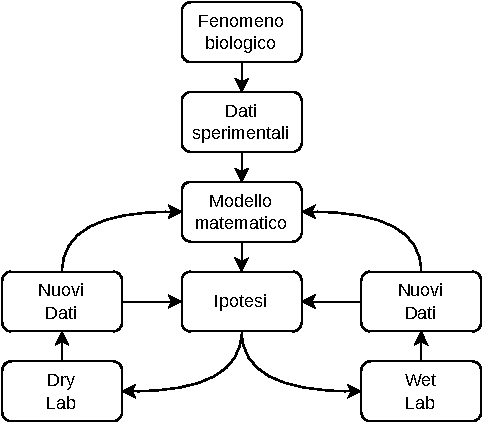
\includegraphics[scale = 0.8]{img/csb.pdf}
  \caption{Grafico rappresentante il processo ciclico della Systems Biology.} 
  \label{fig:csb}
\end{figure}
Un altro aspetto fondamentale del discorso è capire cosa \textbf{non} sia la
\textit{systems biology}. Citando Wolkenhauer \footnote{O. Wolkenhauer, Why
  Systems Biology is (not) called Systems Biology, BIOforum Europe 4/2007}:
\begin{center}
  \textit{Opening then the book, which I discovered in the London bookstore, I
    read the contents list: “Shotgun Fragment Assembly”, “Gene Finding”, “Local
    Sequence Similarities”, ... What?? ... “Protein Structure Prediction”, “Some 
    Computational Problems Associated with Horizontal Gene Transfer” ... what on
    earth has this to do with systems biology, I asked myself?}\\
  \textit{...}\\
  \textit{Most important to me is
    however that cells and proteins are interacting in space and time, that
    is, we are dealing here with (nonlinear) dynamic systems. If you ask me
    then, systems biology is a merger of systems theory with cell biology.}
  \\
  \textit{...}\\
  \textit{Systems biology and bioinformatics are different but complementary.}
\end{center}
Infatti tematiche come l'assemblaggio, l'allineamento etc$\ldots$ non sono
tematiche della \textit{systems biolog}y ma della \textit{bioinformatica},
nonostante spesso vengano confuse e sovrapposte. L'analisi diretta dei dati
biologici non è campo della \textit{systems biology} in quanto si perde uno
degli aspetti fondamentali, ovvero quello del \textbf{tempo}, che comporta lo
studio di \textbf{sistemi dinamici}, che appunto di evolvono nel tempo. In
bioinformatica d'altro canto si ha spesso a che fare con dati provenienti da
pochi timestamp (se non direttamente da uno solo). Inoltre, sempre in
bioinformatica, si studiano solitamente poche componenti biologiche, senza
studiarne l'interazione tra esse.\\
La domanda più importante della \textit{systems biology}, della quale possiamo
vedere uno schema generale delle fasi in figura \ref{fig:csb2}, è quindi:
\begin{center}
  \textit{dato un sistema biologico d'interesse, di cui si vogliono studiare le
    funzioni etc$\ldots$, quale approccio modellistico è più adatto per
    descrivere quel sistema?}
\end{center}
Una volta risposto a questo quesito bisogna ovviamente capire quale sia lo
strumento computazionale di cui si ha bisogno per simulare e analizzare tale
sistema. Bisogna infine capire quali predizioni si possono ottenere da questo
modello, che comunque deve prima essere validato. Tra le cose principali che si
vogliono capire abbiamo, ad esempio, se si può controllare il sistema e se si
può riprodurre il tutto in laboratorio riducendo il numero di tentativi e di
conseguenza anche il costo dell'esperimento in \textit{wet lab}.\\
\begin{figure}
  \centering
  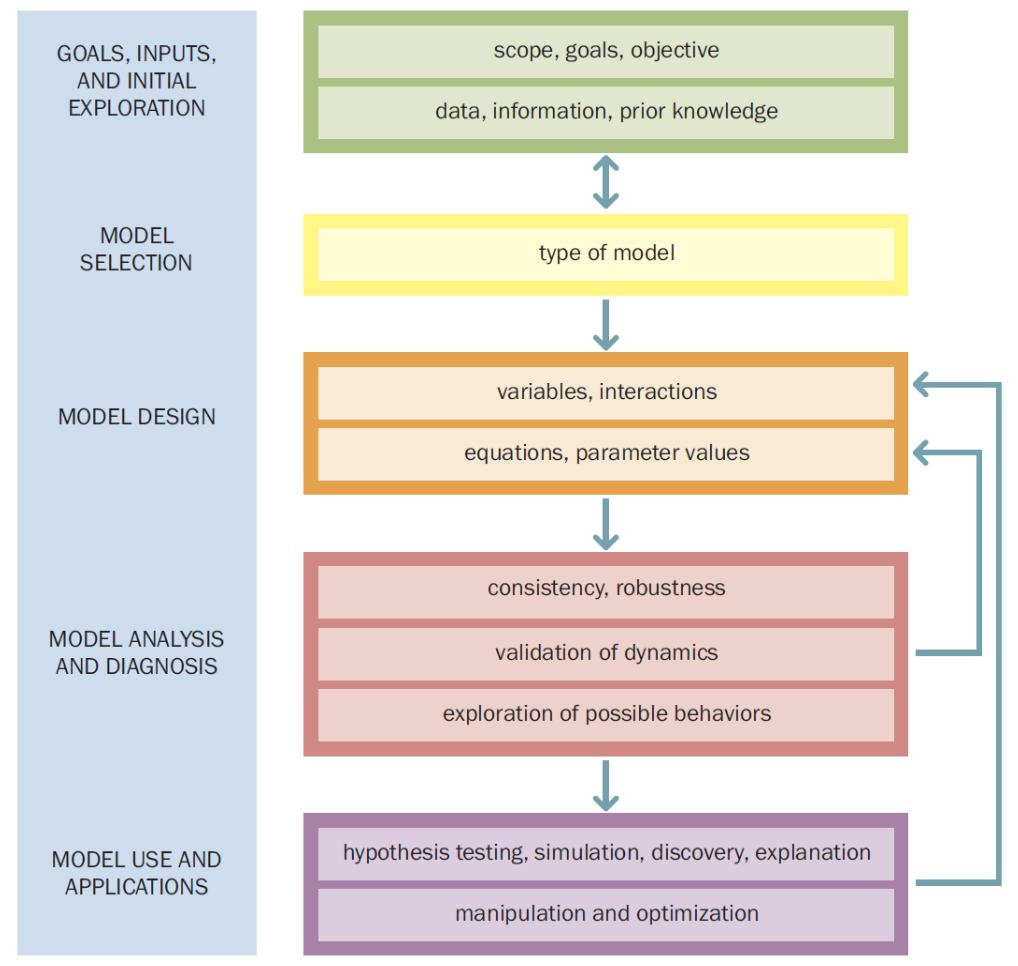
\includegraphics[scale = 0.3]{img/csb2.jpg}
  \caption{Schema generale delle fasi tipiche che compongono la systems
    biology.} 
  \label{fig:csb2}
\end{figure}
Possiamo quindi facilmente intuire che uno degli aspetti fondamentali di questo
ambito è quello di fare le corrette \textit{assunzioni}. Citando ancora
Wolkenhauer \footnote{O. Wolkenhauer, Why Systems Biology is (not) called
  Systems Biology, BIOforum Europe 4/2007}:
\begin{center}
  \textit{The modelling process itself is more important than the model. The
    discussion between the experimentalists and the theoretician, to decide
    which variables to measure and why, how to formally represent interaction in
    a mathematical form is the basis for succesful interdisciplinary research in
    Systems Biology. In light of the complexity of moleculr systems and the
    available experimental data, Systems Biology is the art of making the right
    assumptions in modelling.}
\end{center}
si nota come il raggiungimento delle assunzioni stesse per ottenere il modello
sia una fase di importanza maggiore rispetto al modello stesso. Il modello
infatti rappresenta la realtà ma non è la realtà stessa e partire da assunzioni
false ed errate porterà ad un modello magari funzionante ``dal punto di vista
sintattico'' ma non `` dal punto di vista semantico'', avendo che esso non potrà
mai essere validato. Nella citazione si parla inoltre di \textit{variabili},
come elemento base dei vari modelli. Tra tali variabili si cercano relazioni,
correlazioni etc$\ldots$\\
Normalmente il punto di partenza sono i \textit{dati omici}.
\begin{shaded}
  Quanto qui riportato è tratto da wikipedia
  (\url{https://it.wikipedia.org/wiki/-omica}) 
  \begin{definizione}
    In biologia molecolare, ci si riferisce comunemente al neologismo omica (in
    inglese omics) per indicare l'ampio numero di discipline biomolecolari che
    presentano il suffisso ``-omica'', come avviene per la genomica o la
    proteomica. Il suffisso correlato -oma (in inglese -omes) indica invece
    l'oggetto di studio di queste discipline (genoma, proteoma).  
  \end{definizione}
  I più importanti ``-oma'' proposti recentemente all'interno della comunità
  scientifica sono:
  \begin{itemize}
    \item il \textbf{trascrittoma} è l'insieme degli mRNA trascritti nell'intero
    organismo, tessuto, cellula; è studiato dalla trascrittomica
    \item il \textbf{metabolom}a comprende la totalità dei metaboliti presenti
    in un organismo; è studiato dalla metabolomica 
    \item il \textbf{metalloma} comprende la totalità delle specie di metalli e
    metalloidi; è studiato dalla metallomica 
    \item il \textbf{lipidoma} comprende la totalità dei lipidi; è studiato dalla
    lipidomica 
    \item l'\textbf{interattoma} comprende la totalità delle interazioni
    molecolari che hanno luogo in un organismo; un nome che comunemente indica
    la disciplina 
    della interattomica è quello di biologia dei sistemi (systems biology)
    \item lo \textbf{spliceoma} (da non confondersi con lo spliceosoma, il
    complesso di 
    proteine ed acidi nucleici coinvolti nello splicing) comprende la totalità
    delle isoforme proteiche dovute a splicing alternativo; è studiato dalla
    spliceomica
    \item l'\textbf{ORFeoma} comprende la totalità delle sequenze di DNA che
    iniziano con 
    un codone ATG e terminano con un codone di stop (sequenze note come ORF,
    open reading frames). Queste sequenze sono ritenute in grado di codificare
    per una proteina o per una parte
    \item \textbf{textoma}: l'insieme della letteratura scientifica disponibile
    alla consultazione (studiato dalla textomica)
    \item \textbf{kinoma}: l'insieme delle protein chinasi (dall'inglese kinase)
    di una cellula. Esistono pubblicazioni scientifiche che citano il termine
    kinomica 
    \item \textbf{glicosiloma}: correlato alle reazioni di glicosilazione
    (studiato dalla glicosilomica)
    \item \textbf{fisioma}: correlato alla fisiologia (studiato dalla fisiomica)
    \item \textbf{neuroma}: l'insieme delle componenti nervose di un organismo
    (studiato dalla neuromica) 
    \item \textbf{predittoma}: l'insieme delle predizioni di struttura proteica
    \item \textbf{reattoma}: l'insieme dei processi biologici
    \item \textbf{ionoma}: insieme dei nutrienti minerali e degli elementi in
    tracce che si trovano in un organismo 
    \item \textbf{connettoma}: l'insieme di tutti i neuroni e le sinapsi di un
    cervello 
  \end{itemize}
\end{shaded}
Si hanno quindi vari ``livelli'' di studio, al variare dei dati omici, per i
quali variano gli strumenti. Ad esempio:
\begin{itemize}
  \item si ha il \textbf{genoma}, studiato tramite il \textit{sequenziamento},
  la \textit{genotipizzazione} etc$\ldots$
  \item il \textbf{trascrittoma}, ottenuto dopo la \textit{trascrizione},
  studiato tramite \textit{microarrays}, \textit{oligonucleotide chips}
  etc$\ldots$
  \item il \textbf{proteoma}, ottenuto dopo la \textit{traduzione}, studiato
  tramite \textit{proteomica MS-based}, \textit{elettroforesi} etc$\ldots$
  \item il \textbf{metaboloma}, ottenuto tramite le \textit{reazioni}, studiato
  tramite \textit{spettroscopia di massa}, \textit{risonanze magnetiche}
  etc$\ldots$
  \item l'\textbf{interattoma}, ottenuto tramite appunto le varie
  \textit{interazioni}, studiato tramite \textit{screens yeast-to-hybrid}
  etc$\ldots$ 
  \item il \textbf{fenomeno}, ottenuto dopo l'\textit{integrazione} delle varie
  interazioni, studiato tramite \textit{gene inactivations} etc$\ldots$
\end{itemize}
Ognuno di questi ``livelli'' ha una panoramica diversa su quello che sta
accadendo, è accaduto, potrebbe accadere o accadrà ad una certa
cellula. Partendo dalle informazioni dinamiche/cinetiche, ovvero dai dati, e
dalle informazioni strutturali dei vari \textit{pathway} si riesce ad ottenere
la rappresentazione matematica. Ovviamente è impensabile pensare di studiare
tutti i ``livelli'' contemporaneamente ma si può studiare solo una parte del
sistema, studiandone un paio di ``livelli'' o poco più. Inoltre ogni ``livello''
ha associato un suo formalismo matematico, legato alla singola modellazione
matematica. Non sempre tali formalismi sono facilmente integrabili (magari in un
caso ho delle EDO e in un altro dei grafi). Si ha quindi non solo un discorso di
\textit{data integration} ma anche di integrazione dei modelli matematici stessi
e questo non sempre è possibile.\\
Nella realtà, inoltre, prima di scegliere un modello bisogna scegliere
l'\textit{approccio} con cui ottenerlo. Generalmente se ne hanno due in
\textit{systems biology}: 
\begin{enumerate}
  \item l'approccio \textbf{top-down}. In questo caso si parte dalle analisi
  omiche, solitamente con pochissimi timestamp, i cui risultati vengono trattati
  con tecniche bioinformatiche, che riducono anche l'influenza degli errori, per 
  ottenere una \textbf{mappa globale di interazioni}, con le interazioni tra
  migliaia di componenti cellulari, dalla quale si ottiene il
  \textbf{modello predittivo del sistema}. Questo approccio è quindi supportato
  da una grande quantità di dati basati su \textit{high-throughput} e
  \textit{global profiling}
  \item l'approccio \textbf{bottom-up}. In questo caso si parte dalle
  informazioni, prevalentemente di letteratura, le interazioni tra le componenti
  individuali del sistema, cercando magari le concentrazioni o il
  \textit{kinetic-rate}, ovvero la variazione della concentrazione di un
  reagente o di un prodotto nel tempo misurata in moli per secondo
  $\left[\frac{M}{s}\right]$. Tali informazioni potrebbero non essere
  precise. Da  
  queste si formalizza un modello matematico per 
  avere poi comparazioni tra esperimenti e modelli di simulazione, ottenendo
  alla fine il \textbf{modello predittivo del sistema}. Questo approccio soffre
  quindi la mancanza di dati, specialmente di dati quantitativi. Questo
  approccio è più vicino a quello tipico della biologia, avvicinandosi per
  alcuni aspetti al \textit{pensiero riduzionista} (che mira a studiare piccole
  componenti del sistema).\\
  Tale approccio è sicuramente più complesso, per quanto si possa limitare a
  studiare pathway e non l'intero metaboloma, ma per questo anche più
  informativo. 
\end{enumerate}
Ovviamente tali approcci, per quanto sarebbe fantastico, non possono essere
usati in contemporanea. Detto questo solitamente l'approccio top-down studia i
sistemi su larga scala per poi, a volte, procedere con uno studio bottom-up. In
generale comunque la scelta dipende dalla singola situazione. Non esiste un
meglio o un peggio, anche se i modelli generati dall'approccio top-down hanno
generalmente una minor capacità predittiva anche se studiano sistemi più ampi
rispetto all'approccio bottom-up.\\
Bisogna distinguere quindi quali siano le tecniche tipiche della bioinformatica
(ma anche della statistica)
e quali quelle della \textit{systems biology}. L'uso di tecniche per la ricerca
di similarità, correlazioni, causalità probabilistica, clustering (dove si noti
che non ha un ruolo significativo il \textbf{tempo}) etc$\ldots$
non sono di interesse della \textit{systems biology}, che invece è interessata
allo studio delle causalità in cui il \textit{tempo} è intrinseco e
necessario. Questa necessità di avere il \textit{tempo} comporta una maggior
difficoltà nel recuperare i dati e dell'eseguire la sperimentazione ma comporta,
del resto, un forte ``potere di spiegazione e predizione'' da parte del modello
stesso. \\
Vediamo ora qualche definizione di base.
\begin{definizione}
  Definiamo \textbf{modello} come una descrizione rigorosa e assolutamente non
  ambigua di un sistema. Nel dettaglio tale descrizione è ottenuta tramite un
  adeguato formalismo matematico (l'unico per definizione non ambiguo) e un
  adeguato livello di astrazione (importante per non avere informazioni
  ridondanti o inutili nel modello). 
\end{definizione}
\begin{definizione}
  Definiamo \textbf{proprietà/comportamento emergente} ogni
  caratteristica strutturale (quindi di topologia) o dinamica (quindi in
  evoluzione nel tempo) di un sistema che non può essere capita e/o spiegata
  banalmente tramite l'enumerazione delle componenti ma che deve essere derivata
  unicamente come conseguenza delle interazioni tra le componenti stesse del
  sistema. 
\end{definizione}
\begin{definizione}
  Definiamo \textbf{simulazione} come una tecnica ``computer-based'' per
  determinare una qualsiasi caratteristica emergente e/o predire l'evoluzione
  temporale del sistema. 
\end{definizione}
\begin{definizione}
  Definiamo \textbf{metodo computazionale} come una soluzione automatica, basata
  su uno specifico algoritmo, usata per risolvere problemi difficili (da
  intendersi ``difficili'' anche a livello computazionale) e per
  analizzare sistemi in diverse condizioni.
\end{definizione}
Si noti che, come evidenziato da Fawcett e Higginson\footnote{Tim W. Fawcett
  and Andrew D. Higginson, Heavy use of equations impedes communication among
  biologists, PNAS 2012}, l'uso eccessivo dei formalismi matematici rendono
difficile la comunicazione con i biologi, quindi bisogna muoversi di
conseguenza. I modellatori dovrebbero essere preparati a sviluppare nuovi
strumenti matematici e computazionali, invece di ``forzare'' la descrizione e
l'analisi del sistema con un framework preferito e facilmente applicabile (tipo
usare le EDO per tutto a priori). I  biologi sperimentali dovrebbero essere aperti
a progettare nuovi protocolli di laboratorio per identificare tutte le
caratteristiche qualitative e, soprattutto, quantitative che ancora mancano (per
aiutare anche i modellisti). \textbf{La parte più interessante del gioco del
  modellismo non è ciò che il modello permette di capire, ma esattamente ciò che
  non è in grado di spiegare}, infatti, secondo, Box:
\begin{center}
  \textit{essentially, all models are wrong, but some are useful.}
\end{center}
e, secondo Bower e Bolouri:
\begin{center}
  \textit{In fact, all modelers should be prepared to answer the question:
    ``what do you know that you did not know before?'' If the answer is ``that i
    was correct'', it is best to look elsewhere.}
\end{center}
Infatti un modello non solo deve rispondere a quello che già si sa ma deve
predire qualcosa che ancora non si sa (magari anche non funzionando).
\section{PCNA ubiquitylation}
Vediamo brevemente uno studio in cui ha partecipato anche la professoressa
Besozzi dove il non funzionamento del modello ha portato ad una nuova scoperta
scientifica \footnote{
  Flavio Amara, Riccardo Colombo, Paolo Cazzaniga, Dario Pescini, Attila
  Csikász-Nagy, Marco Muzi Falconi, Daniela Besozzi, Paolo Plevani , In vivo and
  in silico analysis of PCNA ubiquitylation in the activation of the 
  Post Replication Repair pathway in S. cerevisiae, BMC 2013 }.\\
In questo studio si cercava di studiare la \textbf{Post Replication Repair
  (\textit{PRR})}, ovvero il principale pathway di tolleranza al danno del DNA
che bypassa le lesioni del DNA durante la \textit{fase S}, che è in citologia
(la branca della biologia che studia la cellula dal punto di vista morfologico e
funzionale) una fase del ciclo cellulare, durante la quale il processo
principale è la sintesi e duplicazione del materiale genetico contenuto nel
DNA. Bombardando il lievito con raggi UV si è quindi studiata la proteina
\textbf{PCNA}, ovvero l'\textit{l'antigene nucleare di proliferazione
  cellulare}. La struttura di tale proteina (di forma a ciambella) è in grado di
assumere una peculiare conformazione la quale le consente di contattare il DNA
(DNA clamp) e di promuovere l'azione della polimerasi durante la replicazione
del DNA \footnote{\url{https://it.wikipedia.org/wiki/PCNA}}. I raggi UV
provocano lesioni che vengono ``trattate'' dalla PCNA. Se ne è quindi
studiata l'\textbf{ubiquitazione}, modificazione post-traduzionale di una
proteina dovuta al legame covalente di uno o più monomeri di ubiquitina. Tale
legame porta, solitamente, alla degradazione della proteina
stessa\footnote{\url{https://it.wikipedia.org/wiki/Ubiquitina}}. La
\textit{mono-ubiquitazione} avviene tramite gli enzimi \textit{Rad6} e
\textit{Rad8} mentre la \textit{poli-ubiquitazione} tramite gli enzimi
\textit{Rad5} e \textit{Ubc13-Mms2}. La prima comporta errori di trascrizione,
in quanto si aveva sintesi di DNA tra le lesioni, formando \textit{mutageni},
mentre la seconda è ``error free''.\\
Si conoscevano quindi i principali attori del fenomeno, ovvero la proteina e gli
enzimi. C'erano varie cose che però non si conoscevano:
\begin{itemize}
  \item l'ordine spazio temporale della cascata delle interazioni delle varie
  proteine, non sapendo anche i tempi di attivazione dei vari enzimi
  \item se il numero di lesioni influenzasse il bilanciamento tra le
  \textit{mono-ubiquitazioni} e le \textit{poli-ubiquitazioni}
  \item se esistesse una soglia relativa al danno che regolasse l'interazione
  tra i due sub-pathway
\end{itemize}
Si è quindi proceduto, in \textit{wet lab}, irradiando il lievito in modo
controllato, misurando \textit{mono-ubiquitazioni} e le
\textit{poli-ubiquitazioni} al passare del tempo (da 0 a 300 minuti) a varie
dosi di UV, e contemporaneamente studiando un modello matematico (tramite le
varie reazioni, rappresentate tramite \textit{prodotti} e \textit{reagenti}) per
effettuare le simulazioni. Si è visto, in laboratorio, che 
le varie forme ubiquitilate di PCNA sono assenti a basse dosi di UV
($5\frac{J}{m^2}$ e $10\frac{J}{m^2}$), mentre ad alte dosi di UV
($50\frac{J}{m^2}$ e $75\frac{J}{m^2}$) entrambi i segnali sono ancora presenti
dopo 5 ore nei \textit{western blot}. La simulazione matematica confermava
quanto stesse succedendo a 
bassi dosaggi ma non riusciva ad ottenere i risultati ad alti dosaggi. Dopo vari
tentativi, rifacendo gli esperimenti (variando enzimi e geni) e sistemando il
modello (tramite \textit{parameter sweeping/estimation, analisi di sensitività})
si è sospettato che il modello fosse in realtà ``corretto'' ma non 
completo, mancava qualche ipotesi. Da qui la scoperta: si ha anche un altro
pathway, il \textbf{Nucleotide Excision Repair (\textit{NER})} che ``assiste''
la \textit{PCNA} quando le cellule sono gravemente lesionate. NER è infatti
attivo nella \textit{fase S} e serve alla \textit{PRR} per funzionare
correttamente \textit{in vivo}. Risistemando il modello con \textit{NER} ed
enzimi annessi le simulazioni hanno funzionato. \\
Questa è la prova che quando un modello non funziona si può ottenere anche una
scoperta scientifica, ed è una delle situazioni (coi giusti limiti) più
interessanti di questa branca di ricerca.
\section{I Sistemi Complessi}
In \textit{systems biology} si ha quindi a che fare con sistemi che vengono
definiti \textbf{sistemi complessi}, ovviamente presi nella loro ``sottoclasse''
relativa ai sistemi biologici.
\begin{definizione}
  Si definisce un \textbf{sistema complesso} come un sistema consistente di un
  certo numero di componenti più o meno semplici che, prese nel loro insieme,
  danno vita ad un \textit{comportamento emergente}, grazie alle loro
  \textit{mutue interazioni}. 
\end{definizione}
In questo contesto assumono importanza tre concetti chiave:
\begin{enumerate}
  \item \textbf{comportamento non lineare}, quindi non facilmente prevedibile
  \item \textbf{sistema aperto}, ovvero dove l'interazione con l'ambiente da
  parete del sistema è una delle caratteristiche da studiare e modellare
  \item \textbf{sistema dinamico}, ovvero si ha che il sistema evolve nel tempo 
\end{enumerate}
Uno dei punti cruciali è inoltre capire che quando si procede alla modellazione
di un certo sistema non si deve modellare anche cosa ci si aspetta da quel
modello. Tale informazione infatti deve scaturire dalle simulazioni del modello
stesso in modo completamente autonomo.\\
Come visto si studiano quindi insiemi di componenti. L'insieme complessivo delle
funzionalità del sistema non è determinato però da una specifica funzione di
ogni componente ma dalle loro interazioni. Si hanno quindi altri due concetti
chiave:
\begin{enumerate}
  \item \textbf{topologia/architettura interna}
  \item \textbf{moduli funzionali}
\end{enumerate}
Anche componenti molto semplici possono dare vita a un sistema complesso.\\ 
Vediamo quindi qualche esempio di sistema complesso:
\begin{itemize}
  \item un esempio ``semplice'' è quello di una \textbf{reazione enzimatica con
    feedback negativo}. In questo caso si hanno una serie di \textit{reazioni
    lineari} che dal legame di un \textit{substrato} portano ad un
  \textit{prodotto}. La complessità viene data dal \textit{feedback negativo} in
  quanto la produzione del prodotto stesso porta il substrato a non  legare. Si
  ha quindi la cosiddetta \textbf{autoregolazione} che rende questo un vero e
  proprio \textit{sistema complesso}, avendo che il comportamento emergente del
  sistema è in realtà difficile da prevedere.\\
  Ovviamente si potrebbe anche assumere il caso meno semplice dove si ha una
  serie di \textit{reazioni non lineare}. \\
  Si può quindi arrivare anche a parlare di casi più ``estesi'', come quello ad
  esempio di un \textbf{pathway metabolico}. Ci sarebbe inoltre un caso,
  seguendo questo filo pensiero, ancora più estremo, ovvero quello del
  \textbf{metabolismo di un'intera cellula}, come visualizzabile nella figura
  \ref{fig:meta}, dove si hanno moltissime parti che 
  nel dettaglio sono lineari ma che si autoregolano a vicenda, ottenendo quindi
  un \textit{sistema complesso} davvero impossibile da studiare.
  \begin{figure}
    \centering
    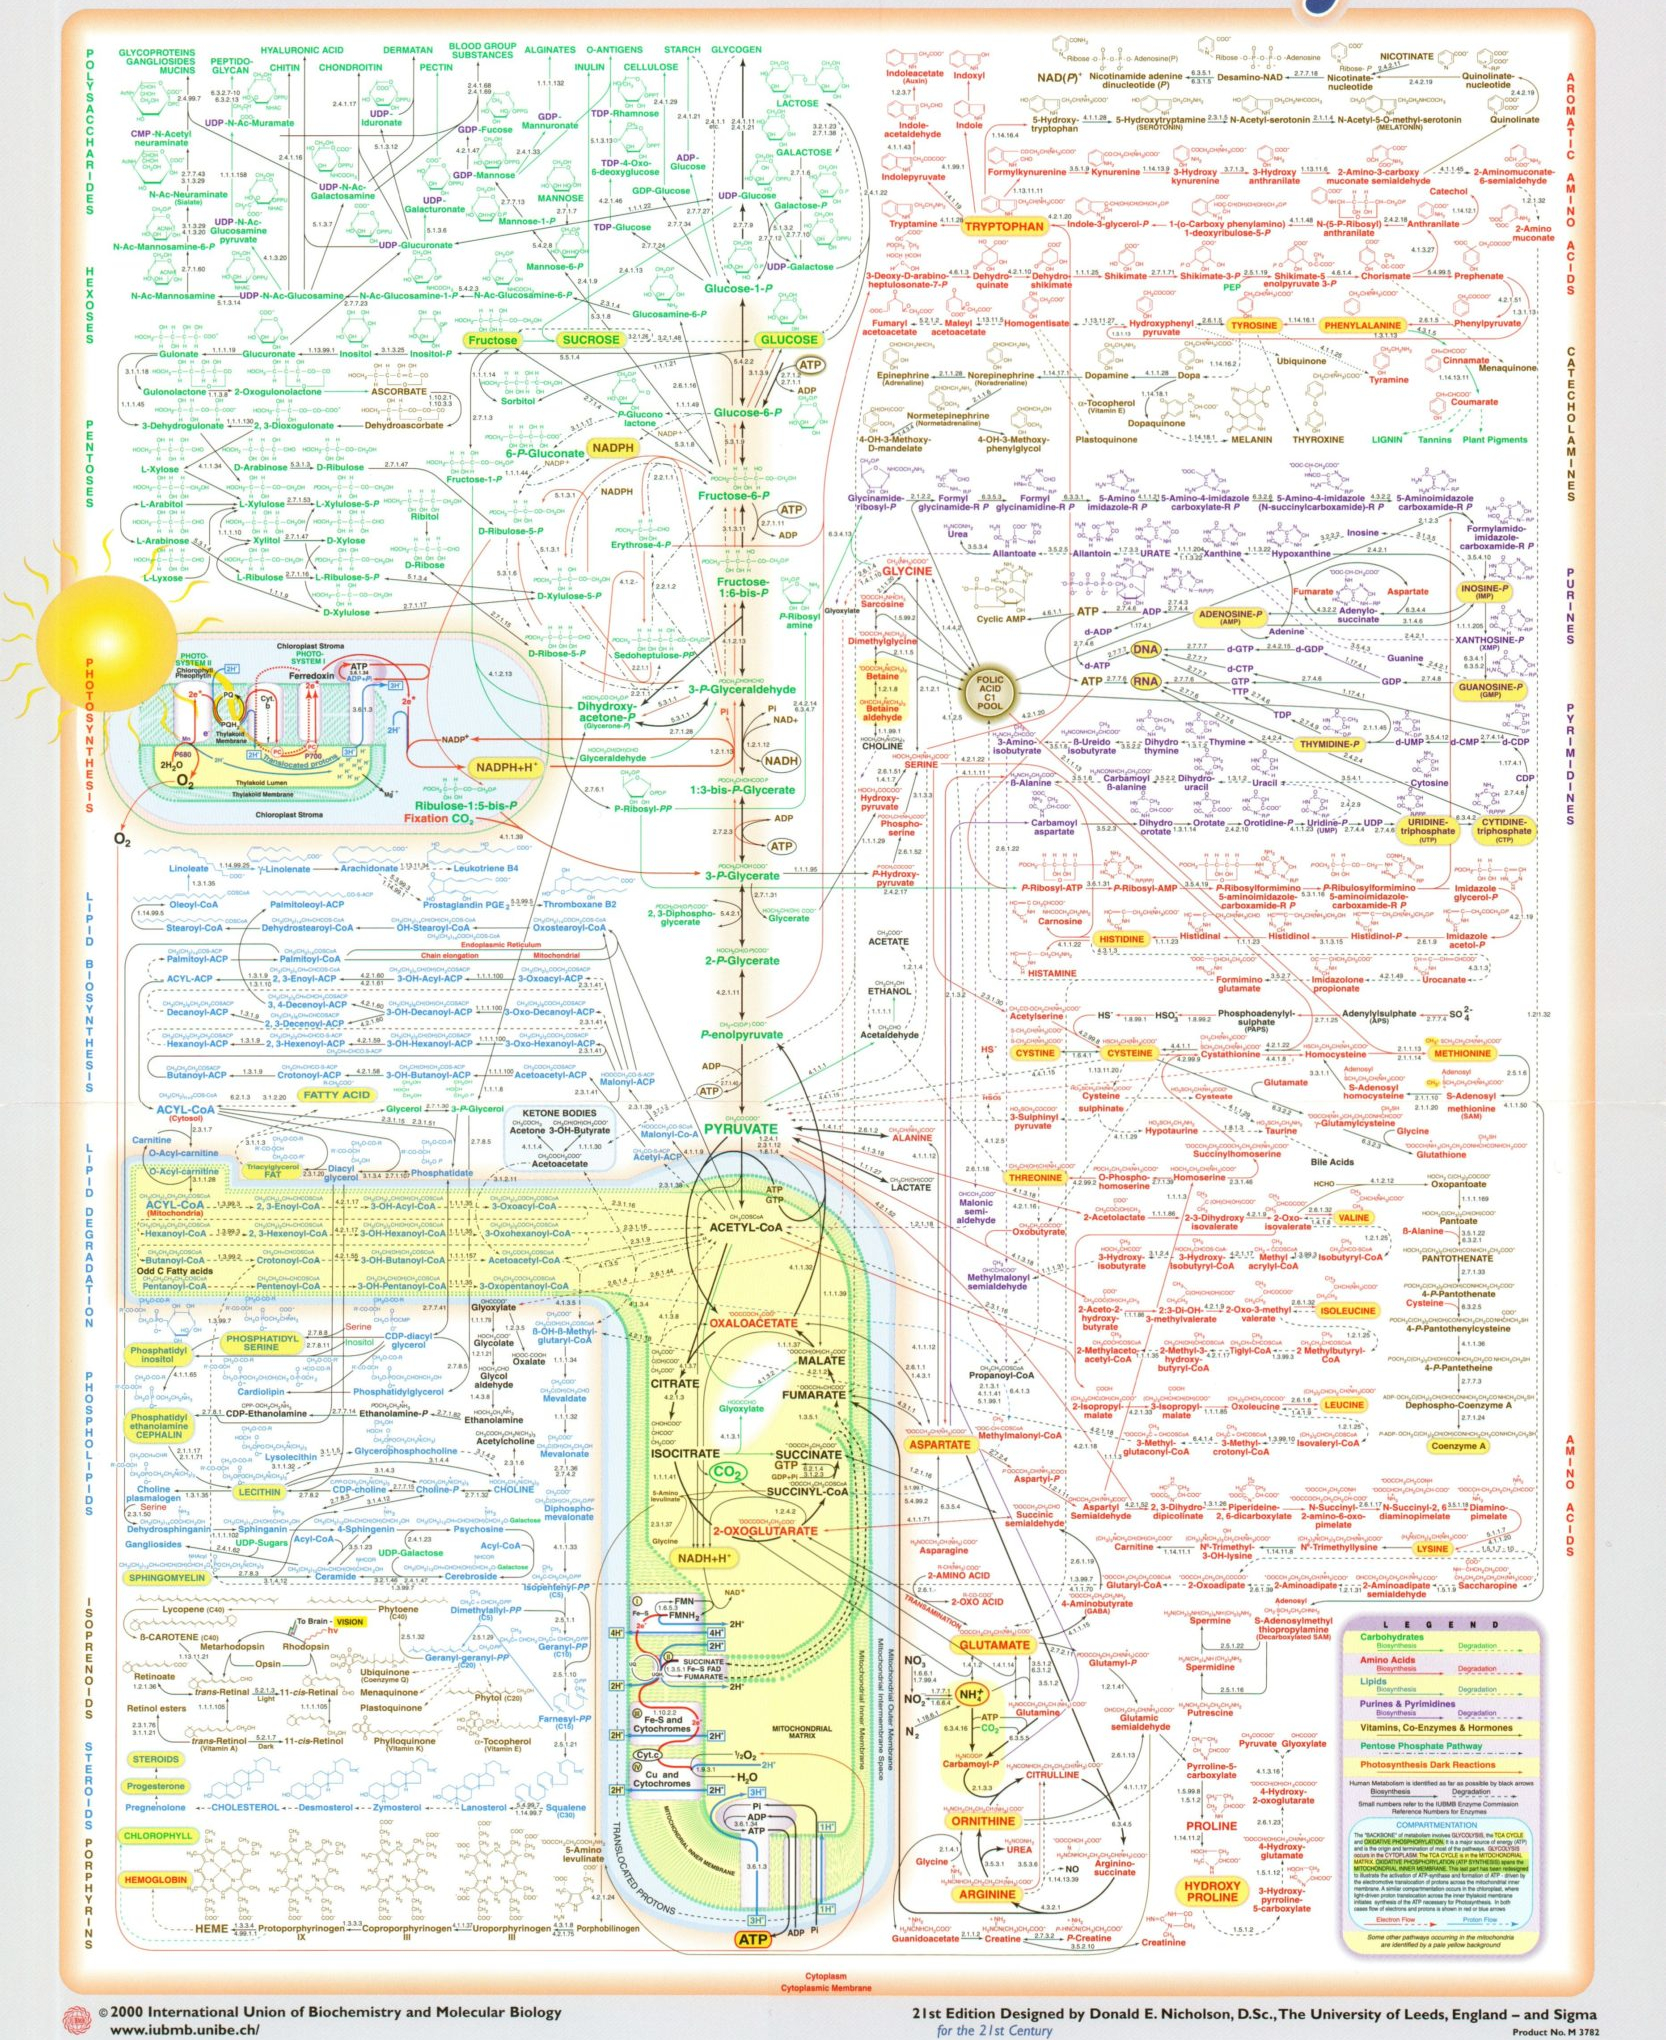
\includegraphics[width = \textwidth]{img/metabolome.jpg}
    \caption{Insieme dei pathway che ``compongono'' il metabolismo di un'intera
      cellula. Tale rappresentazione è stata fatta da Donald E. Nelson,
      dell'università di Leeds e dall'azienda Sigma-Aldrich per la International
      Union of Biochemistry and Molecular Biology del 2000.}
    \label{fig:meta}
  \end{figure}
  \item un altro esempio può essere quello di una \textbf{rete di interazioni
    proteina-proteina (\textit{protein-protein interaction network})} dove si
  hanno:  
  \begin{itemize}
    \item \textbf{nodi} che rappresentano le proteine
    \item \textbf{archi} che rappresentano \textbf{interazioni fisiche} e
    \textbf{interazioni funzionali} tra proteine (???)
  \end{itemize}
  In questo caso la ``complessità'' è data soprattutto dal numero
  incredibilmente alto di proteine (quindi di nodi) e di interazioni tra esse
  (quindi di archi) nel nostro sistema. Un esempio è visualizzabile in figura
  \ref{fig:ppn}. 
  \begin{figure}
    \centering
     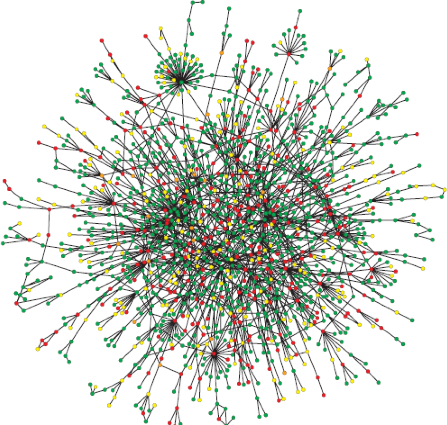
\includegraphics[width = \textwidth]{img/ppn.png}
    \caption{Esempio di rete di interazioni
      proteina-proteina,
      \url{https://www.ebi.ac.uk/training/online/courses/network-analysis-of-protein-interaction-data-an-introduction/protein-protein-interaction-networks/}. In
    tale rete si ha lo studio sul lievito e i vari colori dei nodi rappresentano
    vari effetti fenotipici legati alla rimozione della proteina rappresentata
    dal nodo stesso. Si ha rosso per l'effetto letale, verde per l'effetto non
    letale, arancione per la crescita lenta e giallo per effetto sconosciuto.}
     \label{fig:ppn}
  \end{figure}
  \item un altro esempio è quello delle \textbf{reti di regolazione genica
    (\textit{gene regulatory network})} dove appunto si studiano le relazioni
  che si hanno tra le espressioni e le regolazioni tra geni. In questo caso si
  hanno: 
  \begin{itemize}
    \item \textbf{nodi} che rappresentano i geni
    \item \textbf{archi} che rappresentano le regolazioni tra geni
  \end{itemize}
  Anche in questo caso si possono avere feedback e tali reti sono utili per
  studiare l'\textit{over-espressione di geni}. Inoltre deve essere chiaro che
  la modifica in un certo gene si ripercuote, chi più chi meno, sull'intera
  rete anche se non si ha un singolo gene che ``controlla'' l'intera rete ma
  tutti contribuiscono alla funzionalità dell'intero sistema complesso
  \item aumentando ancora il livello di complessità potremmo pensare allo studio
  di un certo pathway, come ad esempio il \textit{segnale di trasduzione}, in
  una cellula tenendo però conto anche della \textit{componente spaziale},
  tridimensionale, della stessa,  
  nonché le interazioni con l'ambiente. La componente spaziale, che ovviamente
  aggiunge complessità, è una parte rilevante del modello, come il ``movimento''
  al suo interno (prestando sempre attenzione a non aggiungere componenti
  inutili al modello stesso). L'interazione con l'ambiente può portare, ad
  esempio, a \textit{cascate di reazioni intra-cellulari} e a vari ``input'',
  come \textit{ormoni, fattori di sopravvivenza, fattori di
    crescita/anti-crescita, fattori di morte etc$\ldots$} da considerare nel
  modello 
  \item un altro esempio ancor più ``complesso'' può essere quello della
  \textbf{crescita tumorale}, magari ponendo al centro dello studio anche il
  rapporto tra essa e la \textbf{vascolarizzazione}, ovvero la distribuzione di
  vasi sanguigni in un tessuto, in quanto magari si vuole studiare la vicinanza
  tra il tumore e i vasi sanguigni. In questo contesto non solo lo spazio
  tridimensionale è di fondamentale importanza ma bisogna anche modellare
  cellule di vario tipo (normali, cancerogene, legate al sistema immunitario, in
  apoptosi, necrotiche
  etc$\ldots$), che interagiscono in modo diverso tra loro, magari avendo anche
  ``mutazioni'' da normali a cancerogene etc$\ldots$ Si hanno quindi componenti
  eterogenee, dovendo per lo più anche modellare i vasi sanguigni e le
  interazioni con le cellule.
  \item un altro esempio, ``complesso'' almeno quanto il precedente, è lo studio
  della \textbf{formazione di biofilm}, ovvero una aggregazione complessa di
  microrganismi contraddistinta dalla secrezione di una matrice adesiva e
  protettiva. Tale barriera è comunque una struttura permeabile permettendo il
  passaggio dei nutrienti. In un biofilm i microrganismi, tendenzialmente batteri, non solo
  crescono ma, soprattutto quelli più interni e ``protetti'', diventano anche
  più resistenti. Questa è una seria complicazione per la loro eliminazione
  quando fuoriescono dal biofilm. Anche qui quindi bisogna modellare lo spazio
  tridimensionale, l'interazione con l'ambiente, l'interazione tra i vari
  microrganismi (anche se si ha solitamente poca eterogeneità)
  \item cambiando prospettiva un altro esempio di \textit{sistema complesso} è
  quello dello \textbf{sviluppo embrionale e della differenziazione cellulare}
  dove, a partire dall'embrione e da cellule staminali si vanno a formare tutti
  i tipi di cellule che formeranno, ad esempio, i tessuti, gli organi
  etc$\ldots$ dell'uomo. In questo caso solitamente si ha un tipo di
  modellazione diverso, basato su componenti semplici 
  \item un altro esempio è quello dello studio dell'\textbf{ecosistema}. Nel
  dettaglio uno degli aspetti studiati è quello della cosiddetta
  \textbf{dinamica preda-predatore}. Tale dinamica descrive il rapporto tra il
  numero di prede e di predatori e osserva un comportamento oscillatorio (se
  aumentano i predatori diminuiscono le prede fino a che non sono abbastanza per
  i predatori, che calano di numero, portando il numero di prede a crescere
  etc$\ldots$) 
  \item infine un ultimo esempio, molto attuale, di \textit{sistema complesso} è
  quello dello \textbf{studio epidemiologico della diffusione di
    epidemie/pandemie} dove la ``complessità'' è incrementata anche dagli
  aspetti sociali e psicologici delle persone, nonché dalla loro eterogeneità
  anche nel dominio epidemiologico (infetti, gravemente infetti, guariti,
  esposti, suscettibili all'infezione, morti etc$\ldots$)
\end{itemize}
In questi esempi si è spesso parlato più o meno esplicitamente di
\textbf{livelli di complessità}. Per poter avere un'idea di quanti possano
essere bisogna considerare vari punti di vista:
\begin{itemize}
  \item un primo punto di vista è dato dalla \textbf{scala spaziale} dei
  fenomeni che si studiano. Possiamo studiare infatti eventi che accadono nel
  range dei nanometri, o meno, fino a pensare ad eventi in scala umana, in
  metri. Inoltre 
  anche un evento che avviene in nanometri può avere conseguenze visibili in
  metri. Questo tipo di complessità è per lo più un problema matematico dal
  punto di vista della gestione della stessa
  \item un secondo punto di vista è dato dalla \textbf{scala temporale} dei
  fenomeni che si studiano. Anche in questo caso si passa dai nanosecondi, o
  meno, ai miliardi di anni. Un evento quasi istantaneo può avere conseguenze
  evolutive tra milioni di anni. La gestione di questo tipo di complessità è un
  grande problema dal punto di vista computazionale. La complessità aumenta
  all'aumentare della scala temporale
  \item altri livelli di complessità sono dati dai \textit{livelli di funzione
    di un organismo}, avendo, ad esempio, che da \textit{trascrittoma, proteoma}
  e \textit{metaboloma}, in ottica pathway, si passa al \textit{fisioma}, in
  ottica cellule, tessuti, organi e direttamente l'uomo
\end{itemize}
Pensando anche solo alla scala spaziale e quella temporale si ha inoltre che
esse sono in sinergia ma è comunque pressoché impossibile pensare ad un modello
che tenga traccia in modo completo o quasi di entrambe queste scale.
\section{Rappresentazione Grafica}
Ai biologi/biotecnologi etc$\ldots$ piace fare diagrammi e mappe concettuali per
rappresentare graficamente le conoscenze biologiche che hanno su un sistema, ad
esempio componenti molecolari e le loro mutue relazioni, formazione di complessi
molecolari, presenza di feedback di regolazione positivi/negativi
etc$\ldots$. Come si intuisce facilmente diagrammi di questo tipo sono soggetti
ad interpretazioni ambigue e limitano anche l'esplicita rappresentazione della
conoscenza biologica. La matematica è l'unico linguaggio non ambiguo e
fortunatamente esistono anche formalismi, come i \textit{grafi}, le \textit{reti
  di Petri} etc$\ldots$ che non solo sono formalmente rigorosi ma hanno anche
un'interpretazione grafica (tanto amata dalle persone). Ovviamente non sempre si
hanno queste soluzioni intermedie. La modellazione
matematica risolve ogni errata interpretazione e descrive in modo non ambiguo
quello che accade nel sistema e può potenzialmente includere ogni tipo di
ipotesi che può poi essere studiata e testata in \textit{wet lab}. In ogni caso
i diagrammi possono avere utilità nella fase preliminare di discussione tra il
biologo e il modellista: può essere un buon punto di partenza ma non sarà mai
sufficiente per modellare il sistema, che si può ottenere solo con la
formalizzazione matematica di componenti e interazioni. Un esempio è
visualizzabile in figura \ref{fig:dia}\footnote{Besozzi D. (2016) Reaction-Based
  Models of Biochemical Networks. In: Beckmann A., Bienvenu L., Jonoska N. (eds)
  Pursuit of the Universal. CiE 2016. Lecture Notes in Computer Science, vol
  9709. Springer, Cham. https://doi.org/10.1007/978-3-319-40189-8\_3}. 
\begin{figure}
  \centering
  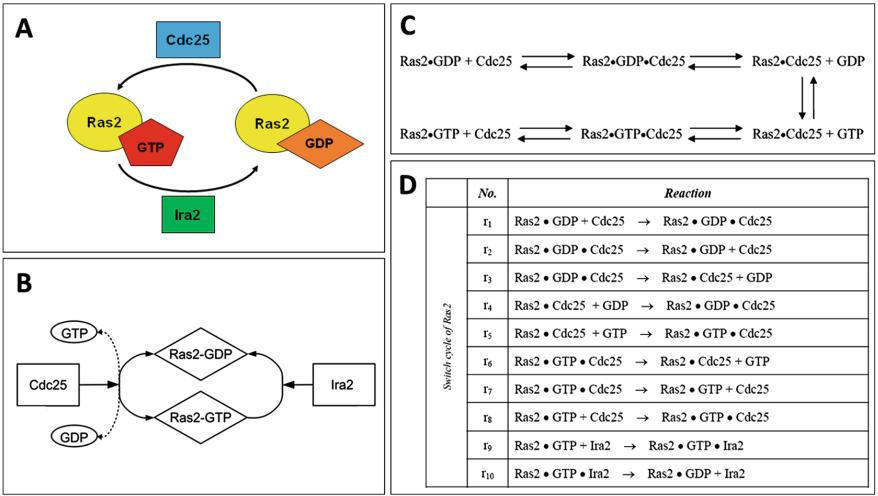
\includegraphics[scale = 0.4]{img/dia.jpg}
  \caption{Esempio (senza entrare nei dettagli biologici che sarebbero ora
    superflui) di un diagramma ambiguo, in figura \textit{A}, tipico 
    dell'approccio biologico. Si hanno poi successive migliorie formali fino ad
    arrivare al modello matematico preciso, in figura \textit{D}, e non ambiguo
    formato da 10 reazioni biochimiche.} 
  \label{fig:dia}
\end{figure}
\section{Tipologie di Modelli}
Sistemi biologici differenti necessitano di approcci modellistici differenti,
ovvero di framework matematici, quindi ad un preciso formalismo, e
conseguentemente computazionali diversi. Inoltre bisogna sempre tenere in
considerazione che ogni metodo computazionale legato ad un preciso modello può
rispondere solo a certe tipologie di domande. Non si ha però una corrispondenza
biunivoca tra ogni approccio modellistico e ogni sistema biologico, infatti
diversi modelli potrebbero prestarsi bene ad un certo sistema biologico (anche
se alcuni modelli sono inapplicabili per certi sistemi biologici o per certe
domande su tali sistemi). La scelta del modello è quindi fortemente legata alle
entità che si vogliono rappresentare e alle risposte che si vogliono ottenere
dal modello. \textbf{Non si ha una strategia universalmente valida per scegliere
il miglior approccio modellistico in base al sistema biologico d'interesse.}\\
Il primo passo è quindi l'interazione tra il biologo/biotecnologo e il
modellista. Il primo deve porsi varie domande tra cui:
\begin{itemize}
  \item cosa si sa e cosa non si sa del sistema biologico in questione?
  \item che tipologie di dato di laboratorio sono disponibili?
  \item che tipologie di dato posso misurare effettivamente in laboratorio? 
\end{itemize}
Anche il modellista quindi si deve porre delle domande fondamentali, tra cui:
\begin{itemize}
  \item quale formalismo matematico si presta meglio per questo problema?
  \item che strumenti computazionali sono necessari?
  \item che tipo di predizioni mi aspetto dal modello?
\end{itemize}
Queste questioni sono ``in ciclo'' tra di esse e sono la base degli studi in
\textit{systems biology}, dove farsi domande è una parte fondamentale. In merito
all'ultima domanda del biologo è 
interessante notare che un modello \textbf{deve} essere validato in
laboratorio. Qualora non sia possibile, ad esempio un ``caso limite'' emerso
dallo studio del modello, non si può fare nulla (anche se, qualora
si avessero più modelli completamente distinti che portano allo stesso risultato
si può presupporre che ci sia un fondo di verità). \\
La domanda fondamentale resta però:
\begin{center}
  \textit{qual è la questione scientifica? Perché mi serve un modello?}
\end{center}
La risposta a questa domanda deve essere ``sicura'' prima di intraprendere uno
studio di modellazione.\\
Nel dettaglio, durante il corso, si vedranno i quattro approcci modellistici
tradizionali più usati anche se si tratta di una selezione tra la moltitudine
degli approcci presenti:
\begin{enumerate}
  \item \textbf{modelli basati su interazioni (\textit{interaction-based
      models})}
  \item \textbf{modelli basati su vincoli (\textit{constraint-based
      models})}
  \item \textbf{modelli logici (\textit{logici-based models})}
  \item \textbf{modelli meccanicistici (\textit{mechanism-based models})}
\end{enumerate}
In generale dato un certo sistema biologico d'interesse, dopo aver risposto alla
domanda fondamentale e avendo quindi ben chiaro il fine di tale modello, la
scelta del modello stesso viene presa considerando secondo quattro aspetti
fondamentali:
\begin{enumerate}
  \item la \textbf{dimensione del sistema}, data in primis dal numero di
  componenti e dal numero delle interazioni tra esse. Si distinguono, secondo
  questo aspetto, due grandi macro-categorie di sistemi:
  \begin{enumerate}
    \item \textbf{sistemi small-scale}, se siamo nel range delle unità o delle
    decine di componenti/interazioni
    \item \textbf{sistemi large-scale}, se siamo nel range delle centinaia o
    migliaia (se non oltre) di componenti/interazioni 
  \end{enumerate}
  Questo è già un ottimo fattore discriminatorio per la scelta del sistema 
  \item il \textbf{livello di dettaglio} necessario a descrivere in modo
  completo le componenti del sistema e le loro interazioni. Si ricorda sempre
  però che formalizzare informazioni inutili e/o ridondanti comporta solo
  un'inutile spreco dal punto di vista computazionale
  \item il \textbf{tipo} e la \textbf{qualità} dei \textbf{dati sperimentali}
  che sono già disponibili o che si è in grado di produrre all'evenienza con
  precisi protocolli al fine di supportare la fase di modellazione. Tali dati
  possono essere ad esempio \textit{dati omici, western blots} etc$\ldots$
  \item il \textbf{carico computazionale} che l'approccio scelto comporta in
  fase di simulazione e analisi dei dati. Un esempio è quello della
  \textit{dinamica molecolare}, che studia come interagiscono tra loro più
  molecole (o anche il comportamento interno di una sola). Tali studi
  normalmente impiegano settimane per simulare anche range temporali molto
  ridotti e necessitano di molte informazioni che non possono essere trascurate
  per ottenere un modello ed una simulazione realistici. Questa scelta è spesso
  un trade-off nella scelta di \textbf{approcci modellistici quantitativi} e
  \textbf{approcci modellistici qualitativi}.\\
  L'uso di \textbf{super computer}, di \textbf{tecniche di calcolo parallelo su
    GPU} etc$\ldots$ sono molto comuni in \textit{systems biology}
\end{enumerate}
Una misura fondamentale è poi la \textbf{capacità predittiva del modello} che,
se bassa, ci porta a preferire \textit{modelli qualitativi}, se alta invece a
\textit{modelli quantitativi}.\\
Si ha quindi un comodo grafico che classifica le quattro tipologie di modelli
in base a questi quattro aspetti\footnote{Besozzi D. (2016) Reaction-Based
  Models of Biochemical Networks. In: Beckmann A., Bienvenu L., Jonoska N. (eds)
  Pursuit of the Universal. CiE 2016. Lecture Notes in Computer Science, vol
  9709. Springer, Cham. https://doi.org/10.1007/978-3-319-40189-8\_3} in figura
\ref{fig:appro}. 
\begin{figure}
  \centering
  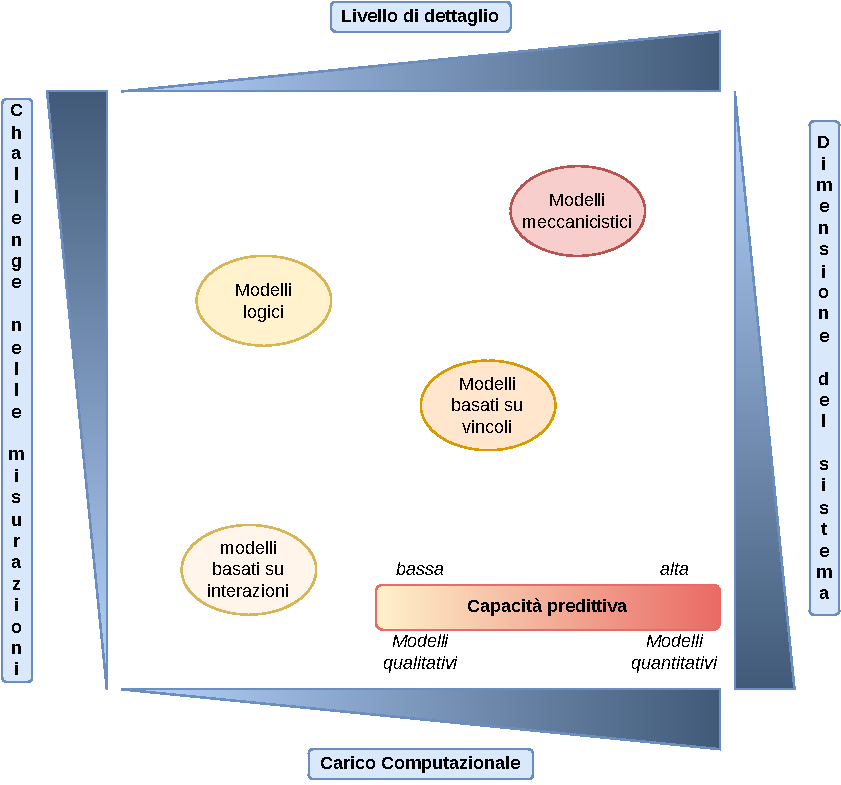
\includegraphics[width = \textwidth]{img/choice.pdf}
  \caption{Schema riassuntivo dei quattro approcci}
  \label{fig:appro}
\end{figure}
Nel grafico notiamo come i \textit{modelli meccanicistici}, tra quelli
analizzati, siano 
quelli con il più alto potere predittivo, che è un aspetto fondamentale ma anche
con i più alti livelli di 
dettaglio, costi computazionali e sfide nella misurazione dei dati
richiesti. L'ovvia conseguenza è che la dimensione del sistema da studiare deve
essere ridotta, avendo quindi \textit{sistemi small-scale}.\\
Si noti che collocare i \textit{modelli logici} non sia così banale in quanto il
livello di dettaglio e la facilità di misurazione possono essere migliorati
usando ad esempio le \textbf{logiche fuzzy}.\\
Un altro aspetto fondamentale da tenere in considerazione è che il processo di
modellazione richiede molto tempo e si basa su continui rifinimenti del modello
stesso, in un processo circolare, come visualizzabile in figura
\ref{fig:cyc}\footnote{Chou IC, Voit EO. Recent developments in parameter
  estimation and structure identification of biochemical and genomic
  systems. Math
  Biosci. 2009;219(2):57-83. doi:10.1016/j.mbs.2009.03.002}. Quindi partendo dai
dati biologici si abbozza un primo modello che viene poi continuamente sistemato
tramite nuove ipotesi, altri dati, analisi \textit{in silico} etc$\ldots$ fino
all'ottenimento di un modello validato.
\begin{figure}
  \centering
  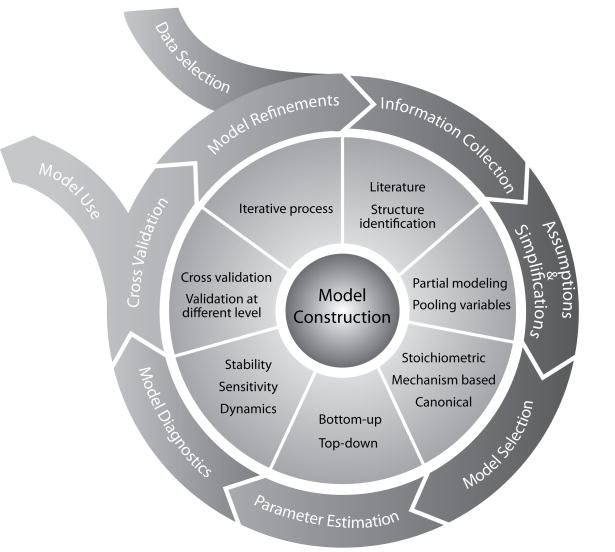
\includegraphics[scale = 0.8]{img/cycle.jpg}
  \caption{Raffigurazione che mostra i dettagli del processo ciclico di
    modellazione in \textit{systems biology}. Molte, ma non tutte, delle keyword
    presenti verranno approfondite nel corso}
  \label{fig:cyc}
\end{figure}
Vediamo ora una breve introduzione ai quattro approcci elencati al fine di poter
fare un confronto tra essi prima di studiarli e formalizzarli nel dettaglio.\\
Prima di fare ciò diamo una più precisa idea dei criteri con cui si classifica
un modello.
\begin{definizione}
  Si definisce \textbf{modello qualitativo} un modello che specifica le
  interazioni tra le componenti del modello stesso.
\end{definizione}
\begin{definizione}
  Si definisce \textbf{modello quantitativo} un modello che assegna un valore ad
  ogni elemento che descrive e anche alle interazioni tra essi. In questo caso
  si possono avere o non avere cambiamenti nel modello.
\end{definizione}
\begin{definizione}
  Si definisce \textbf{modello deterministico} un modello per il quale
  l'evoluzione attraverso i vari stati può essere predetta a partire dallo stato
  corrente, nel dettaglio anche dallo \textit{stato iniziale}. Il comportamento
  evoluzionistico del modello quindi non varierà tra una simulazione e l'altra.
\end{definizione}
\begin{definizione}
  Si definisce \textbf{modello stocastico} un modello che descrive, a partire da
  uno stato corrente, uno stato futuro attraverso una \textit{distribuzione di
    probabilità}.
\end{definizione}
\begin{definizione}
  Un processo è detto \textbf{reversibile/irreversibile} se si può o meno
  procedere in avanti o indietro tra i vari stati.
\end{definizione}
\begin{definizione}
  Con il termine \textbf{periodicità} si intende che il sistema assume una serie
  di stati nell'intervallo di tempo $[t, t+\Delta t]$ ma anche in:
  \[[t+i \Delta t, t+(i+1)\Delta t],\,\,i=1,2,3,\ldots\]
\end{definizione}
\subsection{Modelli Basati su Interazioni}
Questo tipo di modelli vengono usati per \textit{sistemi large-scale} con
centinaia o migliaia di componenti che interagiscono tra loro in modo fisico o
funzionale. Abbiamo vari esempi di questi modelli, tra cui:
\begin{itemize}
  \item \textbf{reti di interazioni proteina-proteina}
  \item \textbf{reti di regolazione genica}
  \item \textbf{reti metaboliche}
  \item \textbf{reti di malattie}, modelli più complessi, modellati tramite un
  particolare tipo di grafo, che sfruttano
  l'integrazione tra \textit{reti di regolazione genica} e grafi/reti
  rappresentanti le malattie e le relazioni tra esse. Si ottiene quindi un grafo
  che mette in relazione componenti genomiche e malattie
\end{itemize}
In questo caso la scelta del formalismo matematico ricade principalmente sulla
\textbf{teoria dei grafi} e si ha quindi un \textit{modello qualitativo} e
\textit{statico}. Infatti il \textit{tempo} non viene considerato in tali
modelli, che di conseguenza non permettono di ottenere informazioni su
eventuali \textbf{comportamenti emergenti}. Non si possono nemmeno ottenere
informazioni quantitative.\\
Parlando di \textit{modelli basati su interazioni} non si può propriamente
parlare di ``simulazioni'' vere e proprie in quanto in primis manca la
modellazione del \textit{tempo} ma anche di altri fattori come il
\textit{kinetic rate}. Inoltre tali modelli difettano anche di una qualsivoglia
modellazione dello \textit{spazio}. Il fulcro dello studio di tali modelli
quindi solitamente si concerta sulle proprietà ``architetturali'' della
struttura della rete, studiando, ad esempio:
\begin{itemize}
  \item la presenza di \textbf{hub}, ovvero nodi in cui sono entranti/uscenti un
  gran numero di archi rispetto agli altri nodi della rete
  \item misure di centralità
  \item presenza di \textit{motivi (motifs)} nella rete
  \item la robustezza topologica
\end{itemize}
Tutte queste misure permettono anche di caratterizzare, caratterizzando la
topologia stessa, una rete rispetto ad un
altra. Infatti si vedranno vari tipologie di rete, tra cui:
\begin{itemize}
  \item \textbf{random network}
  \item \textbf{scale-free network}, caratterizzate da una forte
  \textit{robustezza}
  \item \textbf{hierarchical network}
\end{itemize}
\subsection{Modelli Logici}
Questi modelli possono essere usati sia per sistemi \textit{small-scale} che per
sistemi \textit{large-scale} e alcuni degli esempi sono:
\begin{itemize}
  \item \textbf{reti di regolazione gene-gene}
  \item \textbf{pathway di trasduzione del segnale} (che si ricorda essere la
  capacità di una cellula di convertire uno stimolo esterno in una particolare
  risposta cellulare) 
  \item \textbf{differenziazione cellulare}
  \item \textbf{pathway per la morte cellulare programmata}
\end{itemize}
Il primo caso è un esempio di \textit{sistema large-scale} mentre gli altri di
\textit{sistemi small-scale}.\\
Dal punto di vista del formalismo matematico si ha anche qui la \textbf{teoria
  dei grafi}, a cui viene aggiunta la \textbf{logica booleana}, con i classici
operatori logici $\neg,\land,\lor$, o anche,
preferibilmente, la \textbf{logica fuzzy}, che verrà approfondita più avanti. L'idea di base è quella che lo stato
delle componenti è regolato da altre componenti del sistema stesso. I nodi
possono assumere o valore booleano 0/1 o, in logica fuzzy, qualsiasi valore tra
0 e 1 (con varie conseguenze nel loro studio).\\
Tali modelli sono in grado di simulare il tempo, rientrando quindi nella
categoria dei \textit{sistemi dinamici} ma sono anch'essi della tipologia dei
\textit{modelli qualitativi}. Tali sistemi si prestano ad essere sia
\textit{deterministici} che \textit{non deterministici}.\\
Lo studio di tali modelli solitamente consiste, tramite le simulazioni e le
analisi, nel determinare:
\begin{itemize}
  \item \textbf{cicli}, ovvero sequenze finite di stati complessivi del sistema
  che si ripetono
  \item \textbf{attrattori}, ovvero degli \textit{stati finali} che sono
  raggiungibili da qualsiasi stato iniziale e una volta raggiunti sio resta in
  tali stati
  \item \textbf{bacini di attrattori}, ovvero percorsi che partono da stati
  intermedi e che conducono a degli \textit{attrattori}
\end{itemize}
Tendenzialmente si arriva sempre ad un \textit{ciclo} o ad un insieme di
\textit{attrattori}.\\
La ``potenza'' della \textit{logica fuzzy} permette, come detto, anche di
modellare il \textit{tempo}, derivando quindi un comportamento dinamico del
sistema, descrivendo, ad esempio, la variazione nel tempo tra i valori degli
stati di ogni componente.\\
Un esempio semplice di quello che si può ottenere con tali modelli è
visualizzabile in figura \ref{fig:log}\footnote{Wynn ML, Consul N, Merajver SD,
  Schnell S. Logic-based models in systems biology: a predictive and
  parameter-free network analysis method. Integr Biol
  (Camb). 2012;4(11):1323-1337. doi:10.1039/c2ib20193c}. 
\begin{figure}
  \centering
  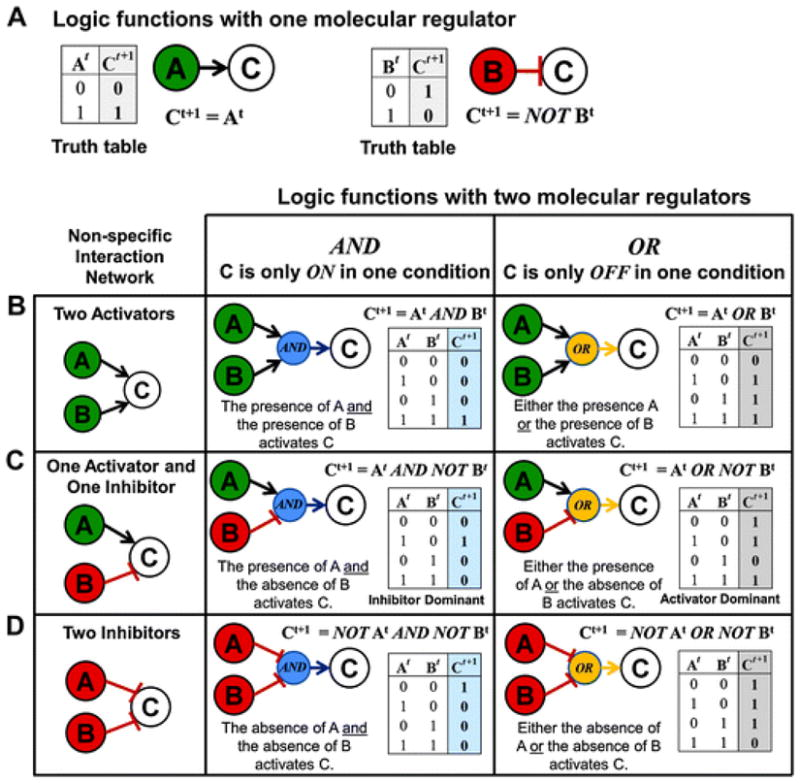
\includegraphics[scale = 0.65]{img/logicnet.jpg}
  \caption{Esempio di modellazione di interazioni tra componenti tramite
    funzioni logiche.}
  \label{fig:log}
\end{figure}
\subsection{Modelli Meccanicistici}
Come già anticipato tali modelli si limitano a descrivere \textit{sistemi
  small-scale}. Questa è la classe di approcci modellistici più complessa ed
eterogenea infatti, in primis, richiede una parametrizzazione completa delle
componenti, con un ampio range di formalismi matematici, tra cui spiccano tra
gli altri i \textbf{metodi numerici} e gli \textbf{algoritmi di simulazione
  stocasitca}. Un problema, già solo 
a questo punto, è che non si hanno spesso i dati per effettuare la
parametrizzazione in quanto i biologi/biotecnologi spesso non sono interessati a
misurarli. \\
Le simulazioni con questi modelli sono usate per studiare l'\textbf{evoluzione
  nel tempo}, quindi la dinamica, del sistema. Si usano metodi
\textit{deterministici, stocastici} e \textit{ibridi}, insieme ad una serie
infinita di altre tecniche computazionali, tra cui l'\textit{analisi di
  sensitività} o il \textit{parameters sweeping}.\\
Si arriva quindi a modelli \textit{quantitativi} e \textit{dinamici}. \\
La scelta tra metodi stocastici, solitamente più dispendiosi, e deterministici
dipende anche dal fatto che \textbf{la vita non è deterministica}. Ad esempio
modellare le interazioni tra, ad esempio tra la proteina \textit{Mdm3} e la
proteina \textit{p53}, avendo che la prima inibisce la seconda, comporta una
funzione molto pulita se studiata in modo deterministico quando in realtà, a
causa di molti fattori, non si ha tale precisione se si va a studiare cosa
accade realmente in natura. Da qui l'uso anche di \textit{modelli stocastici}.\\
La stima dei parametri resta comunque un grandissimo problema e spesso si usano
altre tecniche computazionali/modellistiche in pipeline per inferire gli stessi.
\subsection{Modelli Basati su Vincoli}
Tali modelli sono usati esplicitamente e solo per \textit{sistemi large-scale
  per reti metaboliche}. Il formalismo matematico qui usato si compone di
\textbf{matrici stechiometriche}, \textbf{algebra lineare} e tecniche di
\textbf{ricerca operativa} mentre le
simulazioni e le analisi consistono nello studiare le variazioni nelle
\textbf{distribuzione di flusso}, calcolando i valori di flusso di tutte le
reazioni metaboliche, a seconda di perturbazioni/input prefissati.\\
Non è semplice se si può dire di ottenere dei \textit{sistemi quantitativi} in
quanto si studia il comportamento ad uno \textit{steady state}.\\
Tra gli esempi di uso si hanno:
\begin{itemize}
  \item l'\textbf{ingegnerizzazione metabolica}, ovvero l'ottimizzazione, il
  design e la regolarizzazione di certe strutture/funzioni metaboliche al fine
  di ottenere un certo fenotipo metabolico
  \item studiare \textbf{bersagli di farmaci}, attraverso ad esempio lo studio
  del \textit{rewiring metabolico del cancro}
\end{itemize}
L'idea è quindi quella di:
\begin{itemize}
  \item stabilire dei \textbf{vincoli}
  \item stabilire una \textbf{funzione obiettivo} da
  \textit{massimizzare/minimizzare}
  \item determinare automaticamente la distribuzione dei flussi
\end{itemize}
Si parla di \textbf{Flux Balance Analysis (\textit{FBA})}.
\subsection{Confronto tra i Vari Approcci}
Viste queste prime piccole premesse sui quattro approcci possiamo fare qualche
piccolo confronto. \\
In primis abbiamo capito come lo studio del \textit{tempo} sia assente del tutto
nei \textit{modelli basati su interazioni} e che sia di dubbio uso nel caso dei
\textit{modelli basati su vincoli} a causa dello \textit{steady state}. Quindi
se si dovesse, ad esempio, studiare il cambio di concertazione di una certa
molecola al variare del \textit{tempo} tali approcci sarebbero da scartare a
priori.\\
Si è anche visto come, in realtà, praticamente solo i \textit{modelli
  meccanicistici} ci offrono uno studio quantitativo, al costo di una
complessità sia formale, che di dati, che computazionale molto alta e
riducendosi a studiare solo sistemi piccoli. Ne segue che:
\begin{center}
  \textit{I sistemi meccanicistici sono l'approccio modellistico migliore per
    comprendere e acquisire nuove intuizioni il funzionamento del sistema.} 
\end{center}
Nella realtà però ``avere tutto'' è un'utopia quindi non si ha un vero e proprio
vincitore in questa ``gara tra approcci modellistici'', ben riassunti nella
figura \ref{fig:app}\footnote{Bordbar, A., Monk, J., King, Z. et
  al. Constraint-based models predict metabolic and associated cellular
  functions. Nat Rev Genet 15, 107–120 (2014). https://doi.org/10.1038/nrg3643},
in quanto al variare del problema, dei dati, e di mille altri fattori potrei
aver motivi validi per preferire un approccio ad un altro.\\
\begin{figure}
  \centering
  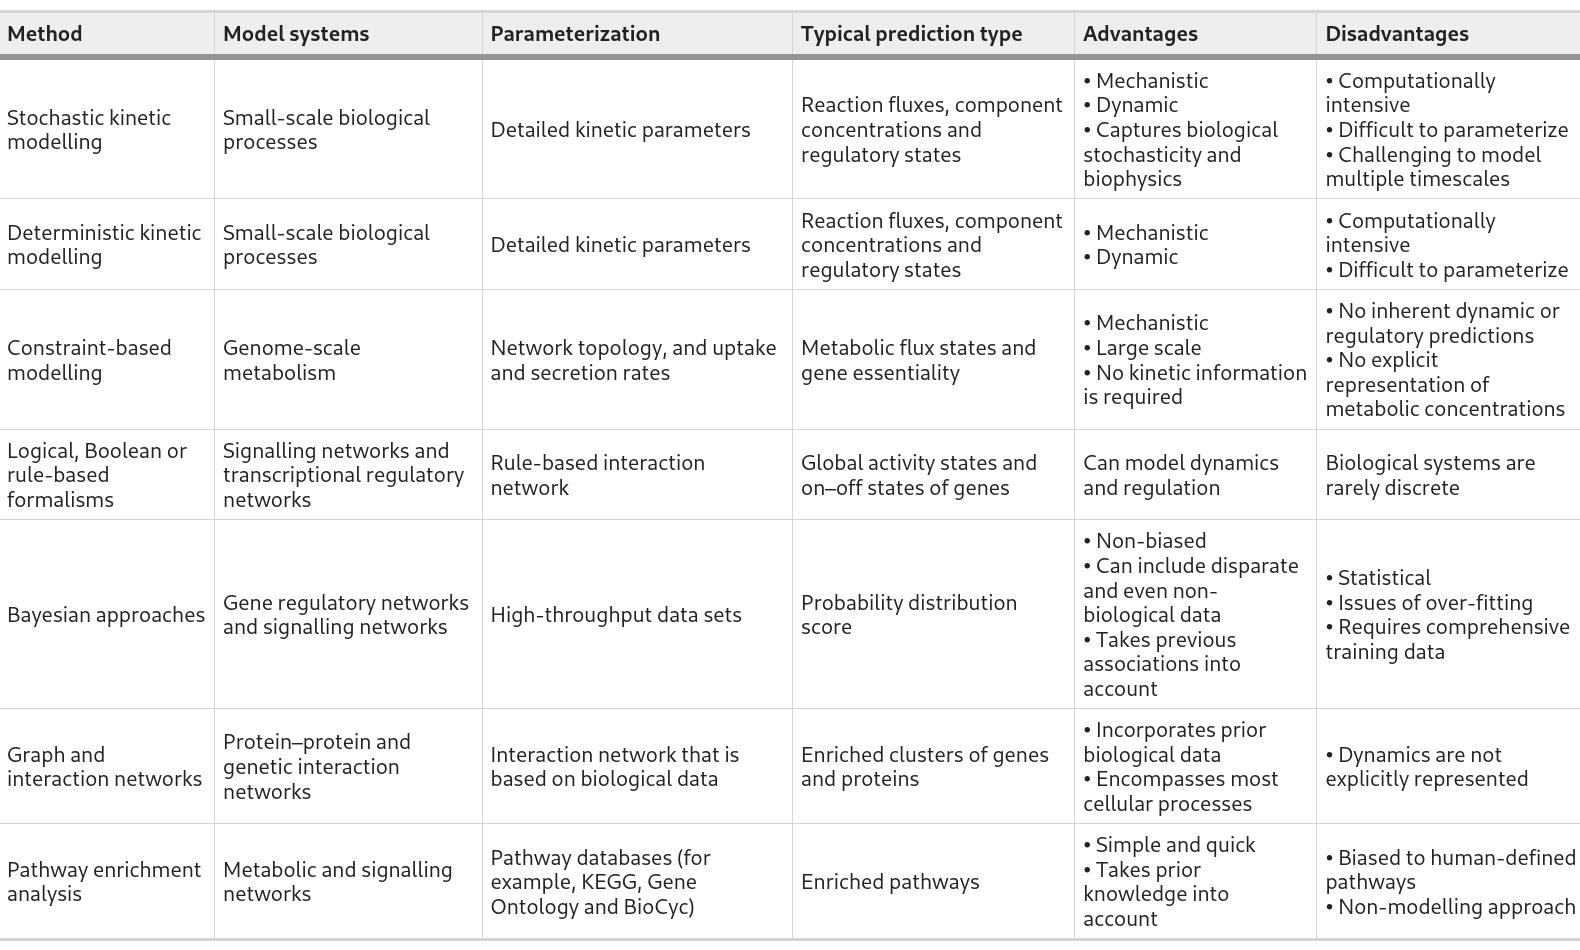
\includegraphics[width = \textwidth]{img/apptable.jpg}
  \caption{Schema riassuntivo delle caratteristiche dei vari approcci.}
  \label{fig:app}
\end{figure}
Inoltre, in questa breve introduzione, si è scoperto come ci siano moltissime
\textbf{dicotomie} in \textit{systems biology}:
\begin{itemize}
  \item \textit{top-down} e \textit{bottom-up}
  \item \textit{qualitativo} e \textit{quantitativo}
  \item \textit{statico} e \textit{dinamico}
  \item \textit{deterministico} e \textit{stocastico}
  \item \textit{discreto} e \textit{continuo} (sia in ottica di
  rappresentazione del \textit{tempo} che della numerazione delle componenti)
  \item \textit{omogeneo} e \textit{eterogeneo}
  \item \textit{a singolo volume} e \textit{multicompartamentale}
\end{itemize}
Tutte queste dicotomie rappresentano la complessità degli studi in
\textit{systems biology}.\\
Integrare i vari modelli è per lo più utopia. Fare \textit{data integration} è
già di per se uno scoglio complesso ma si aggiunge anche la difficoltà di
integrare vari formalismi matematici. Non si ha il modello ``perfetto'' ma si
può scegliere bene in base al sistema biologico da studiare, magari integrando
anche qualche (molto pochi) approccio modellistico diverso, come visibile in
figura \ref{fig:pap}\footnote{Gonçalves E, Bucher J, Ryll A, et al. Bridging the
  layers: towards integration of signal transduction, regulation and metabolism
  into mathematical models. Molecular Biosystems. 2013 Jul;9(7):1576-1583. DOI:
  10.1039/c3mb25489e. PMID: 23525368. }. Nel diagramma si segnala il paper
centrale di Karr et al.: \textit{A whole-cell computational model predicts
  phenotype from genotype}\footnote{Karr JR, Sanghvi JC, Macklin DN, et al. A
  whole-cell computational model predicts phenotype from
  genotype. Cell. 2012;150(2):389-401. doi:10.1016/j.cell.2012.05.044} cruciale
nello studio di un approccio misto per modellare il sistema di un'intera cellula
di un piccolo batterio.
\begin{figure}
  \centering
  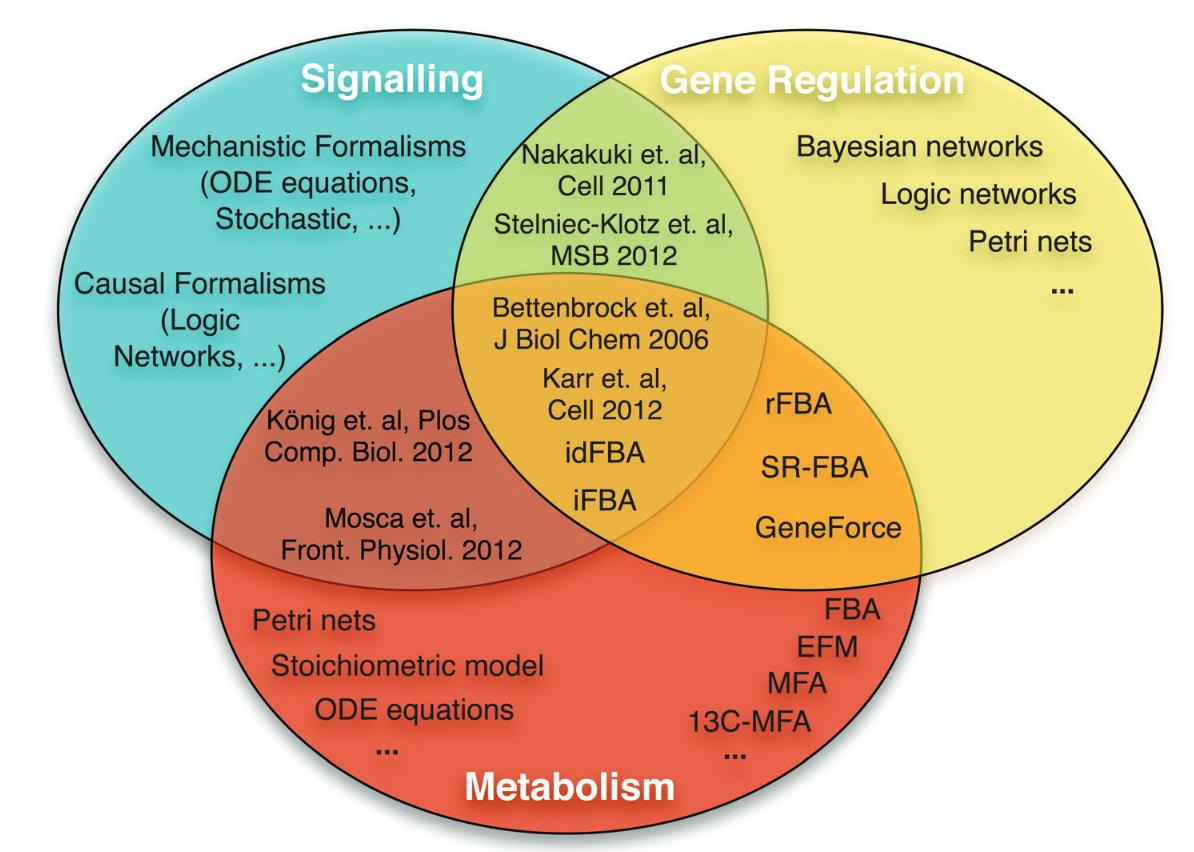
\includegraphics[scale = 0.25]{img/papers.jpg}
  \caption{Diagramma che mostra varie soluzioni modellistiche al variare del
    problema biologico}
  \label{fig:pap}
\end{figure}
\chapter{Interaction-Based Modelling}
Si parte con la descrizione della prima classe di modelli, parlando quindi della
\textbf{interaction-based modelling}.\\
Ricordiamo che tali modelli, come visibile in figura \ref{fig:appro}:
\begin{itemize}
  \item hanno un sistema di grandi dimensioni, con centinaia o migliaia di
  componenti (se non di più),
  essendo quindi \textit{modelli large-scale}
  \item presentano tendenzialmente un basso costo computazionale per le analisi
  \item hanno un basso livello di dettaglio
  \item non presentano particolari difficoltà nella misurazione dei dati
\end{itemize}
Inoltre, sempre ricordando l'introduzione alla classe, questo approccio
modellistico:
\begin{itemize}
  \item non permette propriamente di parlare di simulazioni non modellando
  \textit{tempo, localizzazione spaziale} e \textit{kinetic-rates} 
  \item si indirizzano le analisi verso lo studio topologico della rete
  \item si studiano proprietà emergenti prettamente strutturali quali la
  presenza di \textit{hubs}, misure di centralità, presenza di \textit{motifs} e
  \textit{robustezza topologica} contro certe \textit{perturbazioni}
\end{itemize}
Abbiamo quindi a che fare con \textbf{modelli qualitativi e statici}.\\
Come anticipato possiamo avere vari tipi di relazione tra i nodi della rete in
questo modello, ovvero vari tipi di \textbf{interazioni}.
\newpage
\noindent
Vediamo qualche
esempio\footnote{Merico D, Gfeller D, Bader GD. How to visually interpret
  biological data using networks. Nat Biotechnol. 2009 Oct;27(10):921-4. doi:
  10.1038/nbt.1567. PMID: 19816451; PMCID: PMC4154490.} (\textit{nel corso si
  approfondiranno solo i primi tre esempi, a livello genico e proteico}): 
\begin{itemize}
  \item \textbf{interazioni fisiche}, ovvero interazioni che si verificano tra
  biomolecole a diretto contatto. Ad esempio, le reti proteina-proteina
  con tali interazioni sono importanti in processi come la formazione di
  complessi proteici, la trasduzione del segnale e il trasporto. Sono
  tendenzialmente il caso di studio più semplice
  \item \textbf{interazioni di regolazione}, ovvero interazioni che sono eventi
  di attivazione o inibizione diretta. Ad esempio, nella regolazione
  dell'espressione genica, un fattore di trascrizione è collegato ai suoi
  bersagli da archi diretti nella rete. Quindi posso quindi avere sia
  \textit{regolazioni positive} che \textit{regolazioni negative} e non si hanno
  più \textit{interazioni fisiche}
  \item \textbf{interazioni geniche}, ovvero interazioni che connettono geni la
  cui simultanea perturbazione genetica porta a un risultato fenotipico diverso
  da quello previsto dalla combinazione di singoli effetti. Ad esempio, le
  interazioni letali sintetiche collegano i geni che influenzano debolmente la
  vitalità dell'organismo quando eliminati individualmente, ma sono letali
  quando eliminati in combinazione. Le \textit{interazioni genetiche} sono utili
  per studiare la funzione genica e per identificare complessi e pathway che
  lavorano insieme per controllare le funzioni essenziali  
  \item \textbf{relazioni di similarità}, avendo collegamenti tra oggetti
  biologici che sono \textit{simili} secondo un attributo comune. È possibile
  utilizzare molte diverse misure di somiglianza, come la somiglianza della
  sequenza proteica o la coespressione genica basata su profili trascrizionali
  correlati (avendo sia correlazioni positive che negative). Le relazioni di
  somiglianza sono utili per identificare gruppi di geni o proteine
  funzionalmente correlati. Un altro esempio è quello di studiare se, in una
  certa condizione data, si possono identificare geni indipendenti con un
  profilo di espressione (ovvero escrizione qualitativa e quantitativa
  dell’insieme dei geni trascritti in un dato momento da una cellula o da un
  tessuto, studiabile tramite, ad esempio, l'uso dei
  \textit{microarrays})
\end{itemize}
Quindi in generale si hanno tipi modelli di reti di interazioni associati ai
vari tipi di interazione (fisica, funzionale, genica, etc$\ldots$), ad
esempio\footnote{Winterbach W, Van Mieghem P, Reinders M, Wang H, de Ridder
  D. Topology of molecular interaction networks. BMC Syst
  Biol. 2013;7:90. Published 2013 Sep 16. doi:10.1186/1752-0509-7-90}: 
\begin{itemize}
  \item \textbf{Association networks}, che modellano qualsiasi tipo di relazione
  tra molecole, ad esempio legami, coespressione e somiglianze
  strutturali. Esempi di tali reti sono le \textbf{gene co-expression networks}
  e le \textbf{protein similarity networks} 
  \item \textbf{Functional networks}, che modellano le relazioni funzionali tra
  coppie di molecole (solitamente geni o proteine). Un collegamento implica che
  entrambe le componenti sono coinvolte nella stessa funzione, processo o
  fenotipo. Un esempio sono le \textbf{genetic interaction networks}
  rappresentano interazioni in cui una doppia mutazione 
  porta a un effetto epistatico (che si ha quando una coppia di alleli copre
  l'espressione fenotipica di un'altra coppia di alleli), ad esempio peggiore o
  migliore del previsto rispetto alla singola mutazione 
  \item \textbf{Protein-Protein Interaction (\textit{PPI}) networks}, che sono
  reti non dirette che modellano il legame proteico tra le componenti, che sono
  appunto proteine. Tali reti sono derivate da esperimenti ad alto rendimento
  che utilizzano tecniche come lo \textit{screening di due ibridi di lievito, la
    spettrometria di massa} e la \textit{purificazione per affinità tandem}, che
  sono metodi \textit{high-throughput}. Le
  \textbf{signaling networks} sono correlate alle \textit{reti PPI}
  ma in questo caso i collegamenti sono diretti in base al flusso di segnali
  molecolari
  \item \textbf{Transcription-Regulatory (\textit{TR}) networks}, tali reti sono
  reti bipartite con un insieme di nodi che rappresentano i geni e l'altro che
  rappresenta i \textit{fattori di trascrizione (TF, da ``transcription
    factors'')}. I \textit{TF} sono prodotti di geni (modellati da collegamenti
  \textit{gene-TF}) mentre i geni sono regolati dai \textit{TF} (modellati da
  collegamenti \textit{TF-gene}). I dati per tali reti sono derivati attraverso
  il processo di immunoprecipitazione della cromatina (detto \textit{ChIP}). Le
  \textbf{gene regulatory networks} sono correlate alle \textit{reti TR} ma
  contengono solo geni e i collegamenti rappresentano relazioni regolatorie
  indirette 
  \item \textbf{Metabolic networks}che sono reti bipartite che modellano le
  relazioni tra le reazioni chimiche che si verificano nelle cellule e i
  substrati coinvolti nelle reazioni. Spesso vengono studiate anche reti
  metaboliche ridotte e non bipartite contenenti solo metaboliti o solo
  reazioni. Parlando di metabolismo ovviamente i risultati che ottengo tramite
  queste reti sono diversi da quelli che otterrei usando, ad esempio, un
  \textit{modello basato su vincoli}
\end{itemize}
L'analisi della topologia delle reti è formata quindi da:
\begin{itemize}
  \item la \textbf{teoria dei grafi}, mediante la quale si misura il sistema
  \item le \textbf{misure di centralità}, con le quali si analizza (e non si
  simula) la rete 
  \item la \textbf{classificazione della rete}, ovvero la caratterizzazione
  della sua topologia, e la \textbf{robustezza topologica}, che sono i risultati
  delle analisi. Tali risultati possono anche corrispondere a nuovi ``insight''
  biologici 
\end{itemize}
\textit{Se aggiungiamo funzioni logiche per descrivere come cambia lo stato di
  ogni nodo nel tempo, possiamo effettuare un'analisi dinamica di una rete. Si
  hanno quindi i \emph{modelli basati sulla logica}, che aggiungono complessità,
  sia formale che computazionale, al fine di raggiungere ulteriori risultati.}
\section{Introduzione alle Reti PPI}
Prima di approfondire la classe di modelli si vede un piccolo approfondimento
sulle \textbf{Protein-Protein Interaction (\textit{PPI}) networks}, come
l'esempio in figura \ref{fig:ppn} (anche se si ricorda che la rappresentazione
di un sistema è sempre limitante), anche al
fine di capire il motivo biologico e i limiti tecnici. Gli algoritmi tipici
della teoria dei grafi ci permetteranno di studiarne la topologia.\\
\textit{Questo sarà comunque il modello più studiato in questo corso per questa
  classe}.\\ 
Ovviamente le reti sono formalizzate come dei \textbf{grafi} e, questo caso, si
hanno:
\begin{itemize}
  \item i \textit{nodi} che rappresentano le proteine
  \item gli \textit{archi}, che non sono orientati, che corrispondono alle
  interazioni di legame tra coppie di proteine
\end{itemize}
Come già anticipato le \textit{reti PPI}, più precisamente, parlando di sistemi
\textit{large-scale}, \textbf{large-scale PPI} vengono costruite a partire da
dati proteomici ottenuti tramite metodi \textit{high-throughput}, ben definiti e
con protocolli chiari (per questo non si hanno particolari challenge dal punto
di vista dell'ottenimento dati). Le \textit{reti large-scale PPI} sono però
anche caratterizzate da:
\begin{itemize}
  \item \textbf{conflitti}, in quanto tali reti sono ottenute rappresentando
  tutti i casi possibili, ignorando appunto la componente temporale. Ne segue
  quindi che, in realtà, le interfacce proteiche possono legare molte altre 
  diverse in modo mutuamente esclusivo, avendo magari che alcuni legami possono
  avvenire in modo mutuamente esclusivo in un dato tempo. Rappresentare quindi
  ``tutti i tempi'' può creare ambiguità. L'idea di togliere componenti al
  modello per evitare ambiguità non è una buona idea in quando si toglierebbe
  senso al modello (che già ha poca capacità predittiva)
  \item \textbf{complessità combinatoria} in quanto si ha un'esplosione del
  numero di complessi distinti che possono essere formati da una rete di,
  appunto, ``possibili'' legami
\end{itemize}
Il sistema è quindi \textit{statico}, non cambiando nel tempo, che non viene
nemmeno rappresentato. Il tempo non è comunque un fattore rilevante per gli
studi che si fanno su tali modelli. \\
Si hanno anche alte criticità, ad esempio:
\begin{itemize}
  \item gli archi in una \textit{rete PPI} non rappresentano necessariamente
  connessioni fisiche persistenti, ma piuttosto riassumono le possibilità di
  interazione, come già detto, e quindi si lascia spazio a:
  \begin{itemize}
    \item \textit{gaps} sia per i nodi che per gli archi, ovvero nodi/archi non
    rappresentati in quanto non si conosce una certa interazione (non ancora
    studiata nella letteratura scientifica)
    \item interazioni che sono \textit{false positive} o \textit{false negative}
  \end{itemize}
  \item le interazioni proteina-proteina nell'intera rete non si verificano,
  come detto,
  necessariamente contemporaneamente e/o utilizzando domini di legame diversi
  e/o nello stesso compartimento cellulare. In altre parole il non rappresentare
  dove accade una certa interazione può essere un problema. Si ``pone tutto allo
  stesso livello''
  \item come non si hanno informazioni temporali non si hanno nemmeno
  informazioni quantitative riguardo al funzionamento della cellula, al suo
  stato, al ciclo cellulare etc$\ldots$
  \item si rischia un bias dovuto al fatto che alcune proteine hanno più
  connessioni semplicemente perché sono meglio studiate (si parla, quando si usa
  molto la letteratura come base del modello, di \textbf{literature-curated
    networks}). Un esempio banale è pensare che la proteina \textit{p53}
  compare, a data Marzo 2019, in 94552 paper secondo PubMed (34205 direttamente
  nel titolo) mentre \textit{Snf1} 1037 volte (solo 318 nel titolo)
  \item si hanno forti limiti di modellazione. Ad esempio non si può modellare
  che una proteina interagisca con altre sse queste due hanno prima avuto
  un'interazione tra loro (avendo che il massimo che posso avere è un
  ``triangolo'' nella rete)
\end{itemize}
Possiamo quindi concludere che \textbf{i risultati dello studio di una
  \textit{rete PPI} (ma anche delle altre reti tipiche
  dell'\textit{interaction-based modelling}) non sono sempre così affidabili}.
\section{La Teoria dei Grafi}
Lo studio dei \textbf{grafi} è centrale in vari problemi/tecnologie comuni,
dal web ai social, dalle reti di collaborazione (pensando ad esempio al
\textit{erd\"{o}s number}) a ipotesi come la famosa
\textit{ipotesi dei sei gradi di separazione} che dimostra (come visto sia nel
collegare attori a Kevin Bacon che con lo studio del 1967 più ``accademico''
dello psicologo Stanley Milgram)
come si abbiano di media sei passaggi per collegare due persone a caso nel
mondo. Si parla infatti spesso della \textbf{teoria del mondo piccolo}, che è
appunto una teoria matematica e sociologica che sostiene che tutte le reti
complesse presenti in natura sono tali che due qualunque nodi possono essere
collegati da un percorso costituito da un numero relativamente piccolo di
collegamenti.
\begin{definizione}
  Si definisce formalmente un \textbf{grafo} $G$ come una coppia di insiemi:
  \[G=\langle V, E\rangle\]
  dove:
  \begin{itemize}
    \item $V=\{v_1,\ldots,v_n\}$ è l'insieme dei \textbf{nodi}, di cardinalità
    $n$ 
    \item $E\subseteq V\times V$ è l'insieme degli \textbf{archi}, di
    cardinalità $m$. Si ha che $E=\{e_1,\ldots,e_m\}$, dove un generico arco
    $e_k=(v_i,v_j)$ con $k=1,\ldots,m$, è definito come una coppia di vertici
    $v_i,v_j\in V$ 
  \end{itemize}
\end{definizione}
\begin{definizione}
  In un grafo si definisce \textbf{nodo isolato} un nodo che non è connesso a
  nessun altro nodo. 
\end{definizione}
\begin{definizione}
  In un grafo si definisce \textbf{cappio} un arco tra un nodo e se stesso.
\end{definizione}
\begin{definizione}
  In un grafo $G=\langle V,E\rangle$ si definisce \textbf{percorso/cammino} come
  una sequenza finita o infinita 
  di archi che unisce una sequenza di vertici. Dati quindi due nodi $v_1,v_n\in
  V$ un cammino da $v_1$ a $v_n$ un cammino è una sequenza di nodi: 
  \[(v_1,v_2, \ldots, v_n) \mbox{ tali che }\forall i =1,2,\ldots,
    n-1,\,\,\exists \,e=(v_1, v_{i+1})\in E\]
  Se il vertice di partenza coincide con quello di fine si parla di
  \textbf{ciclo}, quindi $v_1=v_n$. \\
  Ovviamente tra due nodi si possono avere distinti cammini.
\end{definizione}
Il concetto di \textit{cammino} e il concetto di \textit{ciclo} assumono
particolare rilevanza in biologia. I \textit{cicli} servono, ad esempio, per
rappresentare i \textit{feedback} mentre i \textit{cammini}, ad esempio, per le
\textit{vie di trasduzione del segnale} dove si parte da un recettore
transmembrana per poi attivare una catena di reazioni.
\begin{definizione}
  Si definisce \textbf{grafo connesso} un grafo dove esiste un percorso tra ogni
  coppia di vertici. In caso contrario si parla di \textbf{grafo non connesso}.
\end{definizione}
\begin{definizione}
  Si definisce \textbf{grafo completo} o \textbf{grafo completamente connesso}
  un grafo, di $n$ nodi, dove ogni nodo è collegato ai rimanenti $n-1$ nodi.
\end{definizione}
\begin{definizione}
  Si definisce \textbf{grafo totalmente sconnesso} un grafo che non presenta
  archi.  
\end{definizione}
\begin{definizione}
  Due nodi $v_i$ e $v_j$ si dicono \textbf{adiacenti} se esiste un arco, diretto
  o indiretto, $e=(v_i, v_j)$.
\end{definizione}
\begin{definizione}
  Dato un nodo $v$ in un \textit{grafo indiretto} si definisce
  \textbf{grado/connettività/degree} come il 
  numero di 
  nodi adiacenti ad esso. Tale valore solitamente si indica con $k_v$, che è
  ovviamente un numero intero non negativo. Qualora ci sia un cappio esso conta
  doppio.\\
  Un \textbf{nodo isolato} presenta un grado nullo.
\end{definizione}
\begin{definizione}
  Dato un \textit{grafo diretto} si definiscono:
  \begin{itemize}
    \item \textbf{indegree} di un nodo $v$ come il numero di archi entranti in $v$
    \item \textbf{outdegree} di un nodo $v$ come il numero di archi uscenti da $v$
  \end{itemize}
  \textit{In letteratura ha volte si definisce
    \textbf{grado/connettività/degree} in un grafo diretto come la somma di
    \emph{indegree} e \emph{outdegree}}.
\end{definizione}
Nella modellazione di sistemi biologici mediante questa classe di modelli è
interessante notare come si possa passare da un grafo connesso ad uno non
connesso dopo l'influenza di una \textit{perturbazione} sul sistema, che
influisce sulle interazioni (e quindi sugli archi) tra le componenti. Tali
cambiamenti hanno forte valenza dal punto di vista biologico in quanto se un
sistema è propenso a produrre un grafo disconnesso dopo una perturbazione, come
ad esempio in figura \ref{fig:conn}, allora è un sistema che è in generale
propenso a ``fallire''. 
\begin{figure}
  \centering
  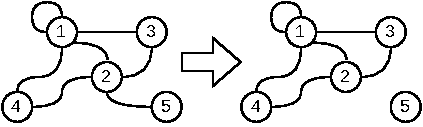
\includegraphics[scale = 1.35]{img/ncon.pdf}
  \caption{Esempio di passaggio da \textit{grafo connesso} a \textit{grafo non
      connesso} dopo un'ipotetica perturbazione, che produce il \textit{nodo
      isolato} etichettato con 5.} 
  \label{fig:conn}
\end{figure}
\begin{definizione}
  Si definisce \textbf{grafo orientato} un grafo dove ogni arco consiste in una
  \textbf{coppia orientata} di vertici, altrimenti si parla di \textbf{grafo non
    orientato}. Formalmente si ha quindi, per un \textit{grafo orientato}, con
  $v_1,v_2\in V$: 
  \[e=(v_1,v_2)\neq e'=(v_2,v_1)\]
  In tal caso, a livello grafico, gli archi sono rappresentati mediante frecce.
\end{definizione}
In questa classe modellistica si hanno:
\begin{itemize}
  \item \textbf{grafi orientati} per \textit{gene regulatory networks} e
  \textit{signal transduction networks}
  \item \textbf{grafi non orientati} per \textit{reti PPI}
\end{itemize}
\begin{definizione}
  Dato un grafo $G=\langle V, E\rangle$ si definisce $S$ come
  \textbf{sottografo} di $G$ come una coppia di insiemi:
  \[S=\langle V', E'\rangle\]
  dove:
  \begin{itemize}
    \item $V'\subseteq V$
    \item $E'\subseteq E$
  \end{itemize}
\end{definizione}
Possiamo quindi dire che, riprendendo la figura \ref{fig:conn}, mediante una
\textit{perturbazione}, si ottiene un sottografo del grafo di partenza. \\
I sottografi sono molto utili per studiare ``caratteristiche'' di forte
interesse biologico, rappresentate appunto da sottografi\footnote{Winterbach W,
  Van Mieghem 
  P, Reinders M, Wang H, de Ridder D. Topology of molecular interaction
  networks. BMC Syst Biol. 2013;7:90. Published 2013 Sep
  16. doi:10.1186/1752-0509-7-90}:  
\begin{itemize}
  \item \textbf{modules} che sono sono sottografi indotti la cui densità di
  archi è elevata rispetto al resto del grafo. Questa non è una vera e propria
  definizione in quanto al natura dei \textit{modules} varia dal contesto e
  dall'algoritmo utilizzato per scoprirli 
  \item \textbf{motifs} che sono piccoli sottografi, solitamente di tre o
  quattro nodi, 
  la cui sovrarappresentazione o sottorappresentazione può indicare che le loro
  strutture sono ``importanti'' o ``dannose'' per il sistema. Di solito, vengono
  contati 
  tutti i \textit{motifs} distinti in una rete, ottenendo una \textit{motif
    signature} per la 
  rete che può quindi essere confrontata con le firme, ottenute campionando da
  un modello nullo di rete casuale appropriato, per determinare la 
  sovrarappresentazione o sottorappresentazione. Le \textit{motif
    signature} possono essere usate per caratterizzare le reti stesse
  \item \textbf{graphlets} che sono simili ai \textit{motifs} ma sono
  \textit{completamente connessi}. Anch'essi vengono utilizzati per costruire
  firme che catturano le caratteristiche locali di una rete  
\end{itemize}
\textbf{Questi argomenti verranno approfonditi più avanti, queste sono solo le
  ``definizioni'' recuperate nel paper indicato.}\\
Torniamo a parlare di della nozione di \textbf{grado}.
\begin{definizione}
  Si definisce \textbf{distribuzione dei gradi/degree distribution} come la
  distribuzione di 
  probabilità dei gradi dei nodi sull'intera rete. Tale distribuzione, denotata
  con $P(k)$, quindi è la
  probabilità che un certo nodo abbia grado esattamente pari a $k$. Tale
  probabilità si ottiene contando il numero di nodi del grafo, denotati $N(k)$,
  che presentano grado $k$ e dividendo tale valore per il numero totale di nodi
  del grafo, che indichiamo con $N=|V|$. Si ha quindi:
  \[P(k)=\frac{N(k)}{N},\,\,k=1,2,\ldots\]
  Avendo una distribuzione di probabilità ne segue che:
  \[\sum_{i=1}^{k_{max}} P(i)=1\]
\end{definizione}
La \textbf{degree distribution} ci permette di classificare un grafo, anche
solo plottando con un istogramma i valori di $P(k)$ al variare di $k$
stesso. Ad esempio qualora si avesse un picco nel plot di tali valori allora si
avrebbe che la rete ha un ``grado caratteristico'' (estremizzando l'esempio
magari si ha una rete dove tutti i nodi hanno grado $k=2$) e quindi non si hanno
nodi fortemente connessi, con alto \textit{degree}. Questo tipo di analisi non
può essere fatta ``visivamente'' su reti reali ma ci si deve per forza affidare
a conti precisi o al più plot della distribuzione stessa. Da tali studi posso
estrarre alcune informazioni, ad esempio:
\begin{itemize}
  \item i nodi con $k=0$, ovvero i nodi isolati possono rilevare che ci sono
  probabilmente informazioni mancanti, falsi negativi etc$\ldots$ mentre il
  valore di $P(0)$ mi dice la probabilità stessa che un qualsiasi nodo della
  rete sia un nodo isolato
  \item i nodi con un $k$ elevato sono tendenzialmente molto pochi e sono i
  cosiddetti \textbf{hubs}, che hanno un ruolo chiave nello studio di
  \textit{reti large-scale} 
\end{itemize}
Al fine di rappresentare i vari valori si usa un piano cartesiano (spesso per
necessità rappresentato in \textit{scala logaritmica}) dove:
\begin{itemize}
  \item l'asse delle $x$ è formato dai valori di $k$
  \item l'asse delle $y$ è formato dai valori di $P(k)$
\end{itemize}
Rappresentando tutte le varie coppie $\langle k,P(k)\rangle$ si ottiene una
``forma'' che è la cosiddetta \textbf{power-law degree distribution} (che
rappresenta la relazione funzionale tra $k$ e $P(k)$ dove una variazione
relativa in una delle due quantità si traduce in una variazione relativa
proporzionale nell'altra quantità, indipendentemente dalla dimensione iniziale
delle due quantità, avendo quindi che una quantità varia come potenza di
un'altra). Lo studio della \textit{power-law degree distribution} è spesso
essenziale nello studio di sistemi biologici.\\
Sempre restando sullo stesso discorso si è notato che in molte reti se si ha un
nodo $v_i$ connesso con un nodo $v_j$, che a sua volta è connesso al nodo $v_h$,
allora è altamente probabile che $v_i$ sia anch'esso collegato al nodo
$v_h$. Questo \textbf{fenomeno di clusering} può essere quantificato usando il
cosiddetto \textbf{coefficiente di clustering}.
\begin{definizione}
  Dato un nodo $v$ si definisce il \textbf{coefficiente di clustering} del nodo
  $v$, denotato con $C_v$, come il numero di archi che connettono nodi adiacenti
  a $v$ diviso il numero totale delle possibili connessioni che si avrebbero tra
  i nodi adiacenti a $v$. Formalmente:
  \[C_v=\frac{2N_v}{k_v(k_v-1)}\]
  infatti si hanno:
  \begin{itemize}
    \item $N_v$ come numero di archi che connettono coppie di nodi adiacenti a
    $v$. Questo valore è facilmente contabile avendo il grafo
    \item $\frac{k_v(k_v-1)}{2}$, parlando di \textit{grafo indiretto}, come
    numero di tutti i possibili archi tra 
    coppie di nodi adiacenti a $v$, che ha grado $k_v$, un valore conosciuto
  \end{itemize}
  Si osserva inoltre che, ricordando che alla fine si ha a che fare con la
  misura di probabilità di quanto sia probabile che si abbia o meno un cluster
  che include il nodo $v$:
  \[0\leq C_v\leq 1\]
\end{definizione}
\begin{esempio}
  Vediamo un semplice esempio che mostra come varia il \textit{coefficiente di
    clustering}. Si studia, nel dettaglio, il valore $C_5$ nei seguenti grafi:
  \begin{figure}[H]
    \centering
    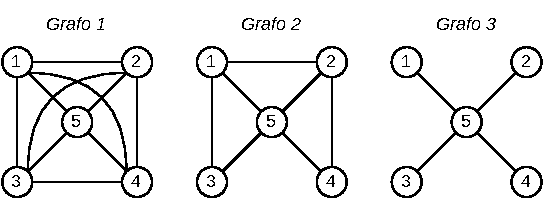
\includegraphics[scale = 1.3]{img/clus.pdf}
  \end{figure}
  In tutti i casi si ha $k_5=4$ ma:
  \begin{itemize}
    \item nel \textit{Grafo 1} si ha $N_5=6$ e $C_5=\frac{12}{12}=1$ e infatti
    il nodo $5$ è sicuramente in cluster
    \item nel \textit{Grafo 2} si ha $N_5=3$ e $C_5=\frac{6}{12}=0.5$
    \item nel \textit{Grafo 3} si ha $N_5=0$ e $C_5=\frac{0}{12}=0$ e infatti il
    nodo $5$ non è sicuramente in cluster
  \end{itemize}
\end{esempio}
Questo tipo di coefficiente è utile soprattutto nel caso di \textit{grafi
  indiretti}. Nel caso di \textit{grafi diretti} bisogna invece ragionare in
ottica di \textit{indegree} e \textit{outdegree}.\\
Un caso limite interessante in ottica di \textit{coefficiente di clustering} è
quello della \textbf{clique}.
\begin{definizione}
  Si definisce \textbf{clique (\textup{cricca})} di un \textit{grafo non
    orientato}
  $G=\langle V,E\rangle$ come un sottoinsieme $V'\subseteq V$ di vertici tale
  che: 
  \[(v_1,v_2)\in E,\,\,\forall \,v_1,v_2\in V'\]
  quindi un sottoinsieme di vertici con solo vertici collegati da un arco.
\end{definizione}
Il caso della \textit{clique} è quindi il ``caso migliore'' parlando del
fenomeno del clustering.\\
Il singolo \textit{coefficiente di clustering} di un nodo comunque non è di
particolare interesse se preso in modo isolato, in quanto si vuole classificare
l'intera rete.
\begin{definizione}
  Si definisce il \textbf{coefficiente di clusering medio}, denotato con
  $\langle C\rangle$, il valore medio di tutti i \textit{coefficienti di
    clusering} dei nodi del grafo.
\end{definizione}
Il \textit{coefficiente di clusering medio} permette di caratterizzare la
tendenza complessiva dei nodi di una rete a formare gruppi o cluster. Questo è
quindi un valore che ci permette di caratterizzare la topologia di una rete.
\begin{definizione}
  Si definisce la funzione $C(k)$, che potremmo chiamare ``\textbf{average
    clustering distribution}'' o \textbf{average clustering coefficient}, come
  la media dei \textit{coefficienti di 
    clusering} di tutti i nodi di grado pari a $k$ nella rete.
\end{definizione}
Il valore $C(k)$ quindi fornisce un'indicazione del carattere
modulare/gerarchico di una rete, ovvero l'esistenza di sottografi/sottoreti
caratterizzati da nodi fortemente collegati internamente, che presentano scarse
connessioni con altre parti della rete.
\begin{definizione}
  Si definisce la \textbf{lunghezza del cammino} tra due nodi $v_1$ e $v_n$ come
  il numero di archi che si hanno nel cammino.\\
  Si definisce \textbf{cammino minimo}, notando che potrebbe non essere unico,
  un cammino di lunghezza minima tra due nodi. 
\end{definizione}
Anche la nozione di \textit{lunghezza del cammino}  ha un ruolo centrale nella
modellazione di sistemi biologici. Basti pensare, in modo comunque approssimato
e semplicistico, che più è lungo il cammino e più sono le interazioni biologiche
e quindi, ad esempio, più energia è richiesta alla cellula. Infatti normalmente
la natura ha fatto sì che ogni ``operazione biologica'' venga fatta nel modo
meno dispendioso possibile, quindi, ricollegando la modellazione a grafo,
mediante \textit{cammini minimi}. Nella realtà si vedrà il concetto di
\textbf{ridondanza} in quanto si hanno vari modi, nel mondo biologico, per
ottenere lo stesso risultato anche se con ``cammini'' di lunghezza diversa
(magari per casi, ad esempio, in cui alla cellula conviene
``temporeggiare''). Inoltre magari ad un percorso più lungo può comunque
corrispondere un dispendio energetico minore. In ogni caso l'aggiunta di
\textbf{pesi} al grafo permette 
una modellazione leggermente più precisa, potendo rappresentare ad esempio, i
``costi'' delle reazioni etc$\ldots$\\
Un'altra cosa interessante da notare nella maggior parte delle reti è che
esiste un cammino relativamente breve tra qualsiasi coppia di nodi e la
lunghezza media di tale cammino è proporzionale al logaritmo della dimensione
della rete, quindi al numero totale di nodi. Questa è la cosiddetta
\textbf{small world property} che sembra caratterizzare la maggior parte delle
reti complesse, comprese \textit{reti metaboliche} e \textit{reti PPI}.
\begin{definizione}
  Si definisce un \textbf{grafo pesato} $G=\langle V,E\rangle$ come un grafo a
  cui viene associata anche una \textbf{funzione di peso} $w$:
  \[w:E\to\mathbb{R}\]
\end{definizione}
Esistono, oltre a quelle già citate, anche altre metriche di studio, tra
cui\footnote{Winterbach W, Van Mieghem P, Reinders M, Wang H, de Ridder
  D. Topology of molecular interaction networks. BMC Syst
  Biol. 2013;7:90. Published 2013 Sep 16. doi:10.1186/1752-0509-7-90}: 
\begin{itemize}
  \item ulteriori \textbf{metriche per i cammini} come il \textit{cammino
    minimo} su \textit{grafi pesati} o il \textit{cammino minimo medio} tra
  ogni coppia di nodi
  \item la \textbf{metrica di centralità} fornisce una classifica dei nodi in
  base alla loro "importanza". La versione più semplice sfrutta appunto il grado
  di un nodo per misurarne la centralità, parlando quindi di \textbf{degree
    centrality}. Un'alternativa è la \textbf{closeness centrality} che è il
  reciproco della somma dei cammini più brevi verso tutti gli altri nodi (cioè
  un nodo la cui \textit{closeness centrality} è alta è vicino a molti
  nodi). Un'ulteriore metrica è la \textbf{betweenness centrality} ovvero la
  frazione di cammini minimi che passano attraverso un nodo. Tra le metriche più
  elaborate si annoverano la \textbf{centralità per autovettori} e il
  \textbf{pagerank} che sono misure della frequenza con cui si arriva a un nodo
  quando si esegue una \textit{random walk} su una rete.  
\end{itemize}
\textbf{Queste non sono comunque metriche solitamente utili per la
  caratterizzazione della topologia di una rete}.
\begin{definizione}
  Si definisce un grafo $G=\langle V,E\rangle$, orientato o meno, come un
  \textbf{grafo bipartito} se:
  \begin{itemize}
    \item l'insieme dei nodi $V$ è in realtà l'unione di due sottoinsiemi di
    nodi $V_1$ e $V_2$, ovvero $V=V_1\cup V_2$, tali che la loro intersezione è
    nulla, ovvero $V_1\cap V_2=\emptyset$
    \item data la prima premessa si ha che ogni arco del grafo connette solo un
    nodo in $V_1$ ad un nodo in $V_2$
  \end{itemize}
  Ad esempio potremmo avere questi casi, dove i primi due grafi sono bipartiti
  (come evidenziato anche a livello visivo dai colori che identificano le
  partizioni) a differenza del terzo (a causa dell'arco in rosso):
  \begin{figure}[H]
    \centering
    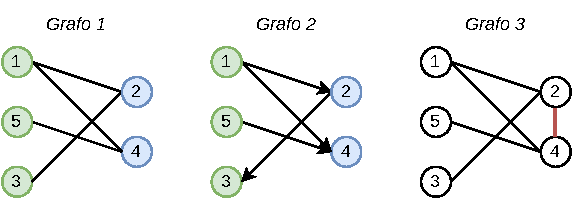
\includegraphics[scale = 1.3]{img/bip.pdf}
  \end{figure}
  Potenzialmente si possono anche avere \textbf{grafi tripartiti}, con 3
  partizioni, o in generale \textbf{grafi multipartiti} con $m$ partizioni.
\end{definizione}
\newpage
Un esempio d'uso dei \textit{grafi bipartiti} sono le \textbf{human desaesome
  networks}, come ad esempio\footnote{Goh, Kwang-Il, et al. "The
  human disease network." Proceedings of the National Academy of Sciences 104.21
  (2007): 8685-8690.}:
\begin{figure}[H]
  \centering
  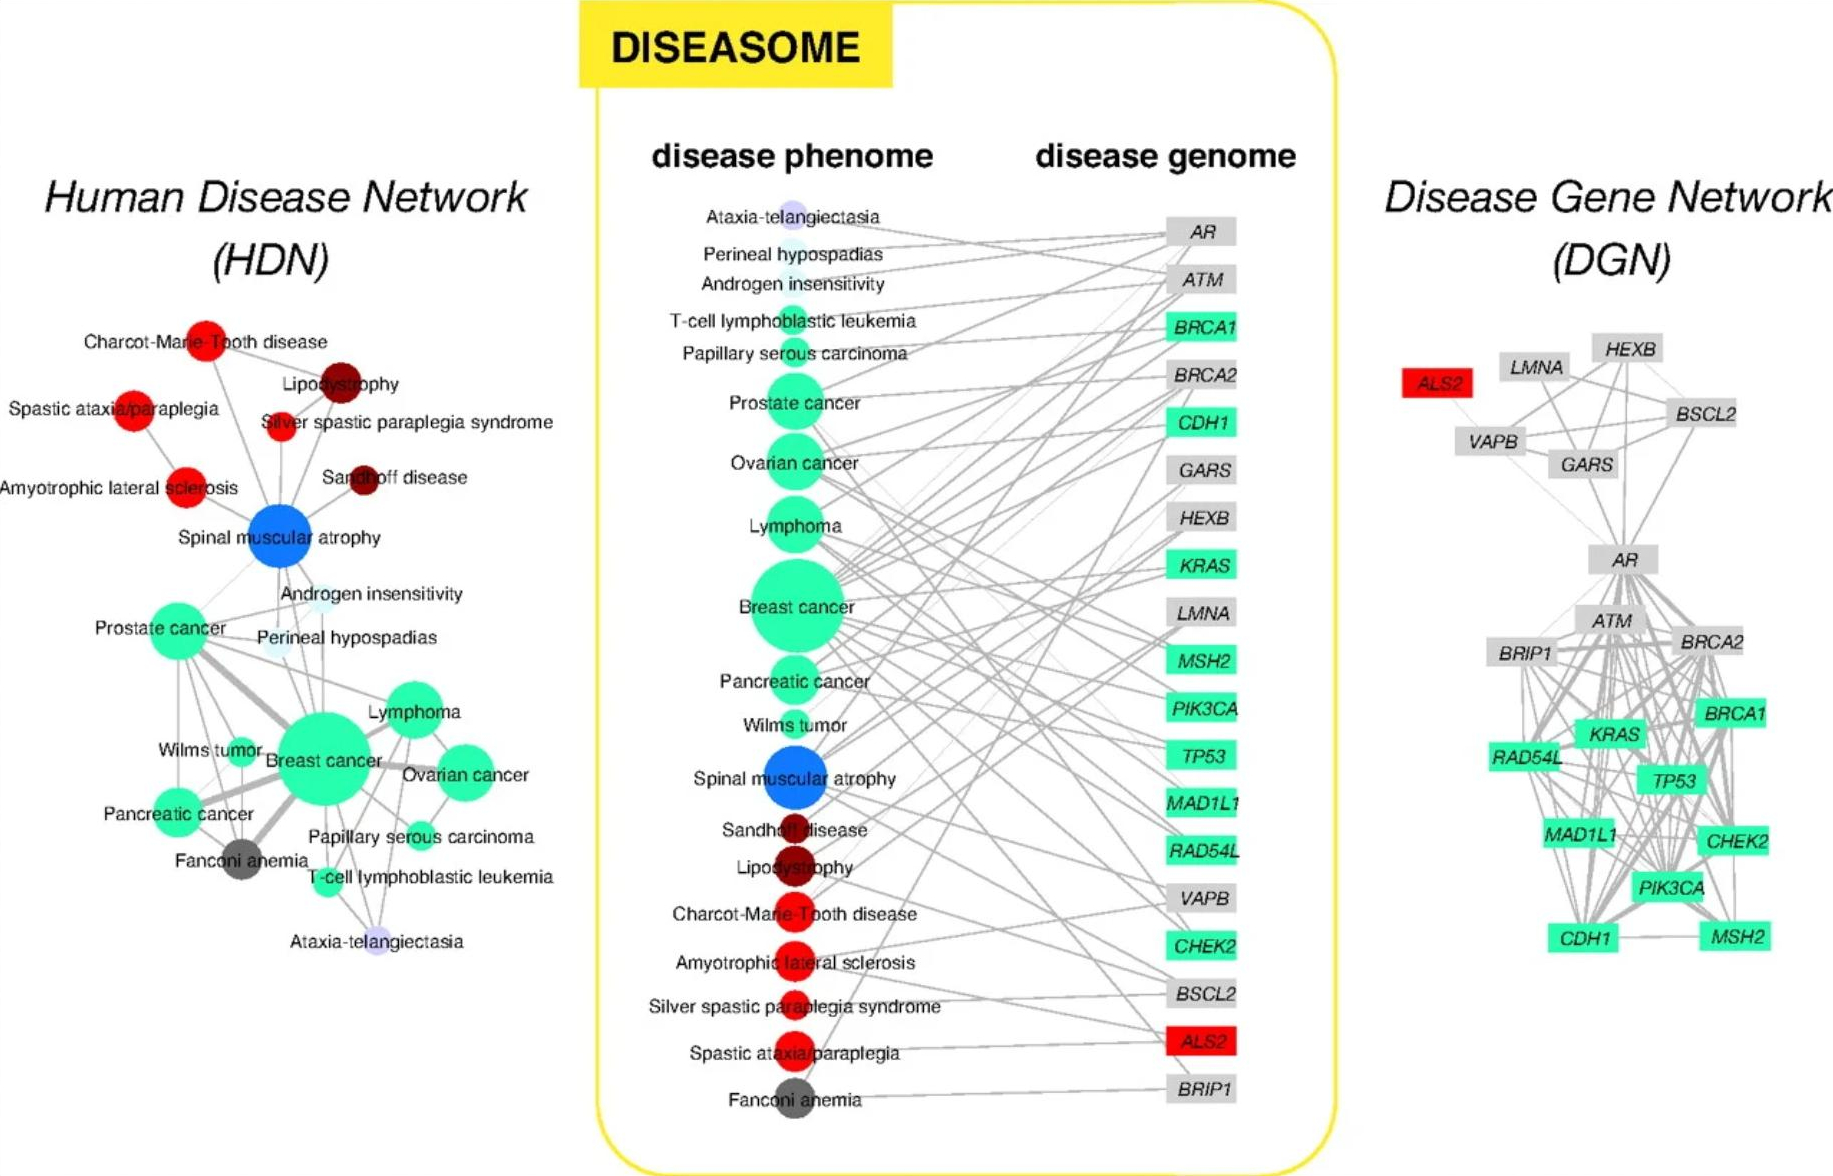
\includegraphics[scale = 0.7]{img/bi.jpg}
\end{figure}
Nella figura si hanno appunto due partizioni: 
\begin{itemize}
  \item un sottoinsieme di nodi per i geni
  \item un sottoinsieme di nodi per le malattie
\end{itemize}
Banalmente quindi un nodo che rappresenta una malattia è legato a un nodo che
rappresenta un gene se è noto che una
mutazione di quel gene induce l'insorgenza di quella malattia. A supporto posso
inoltre avere due ulteriori reti solo per i geni e solo per le malattie.\\
Un esempio di rete basata su un \textit{grafo multipartito} è, ad esempio, una
\textbf{drug-target protein network}, come quella proposta da
Nacher visualizzabile in figura
\ref{fig:mbip}\footnote{Nacher, J., Akutsu, T. Structural controllability of
  unidirectional bipartite networks. Sci Rep 3, 1647
  (2013). https://doi.org/10.1038/srep01647}.
\begin{figure}
  \centering
  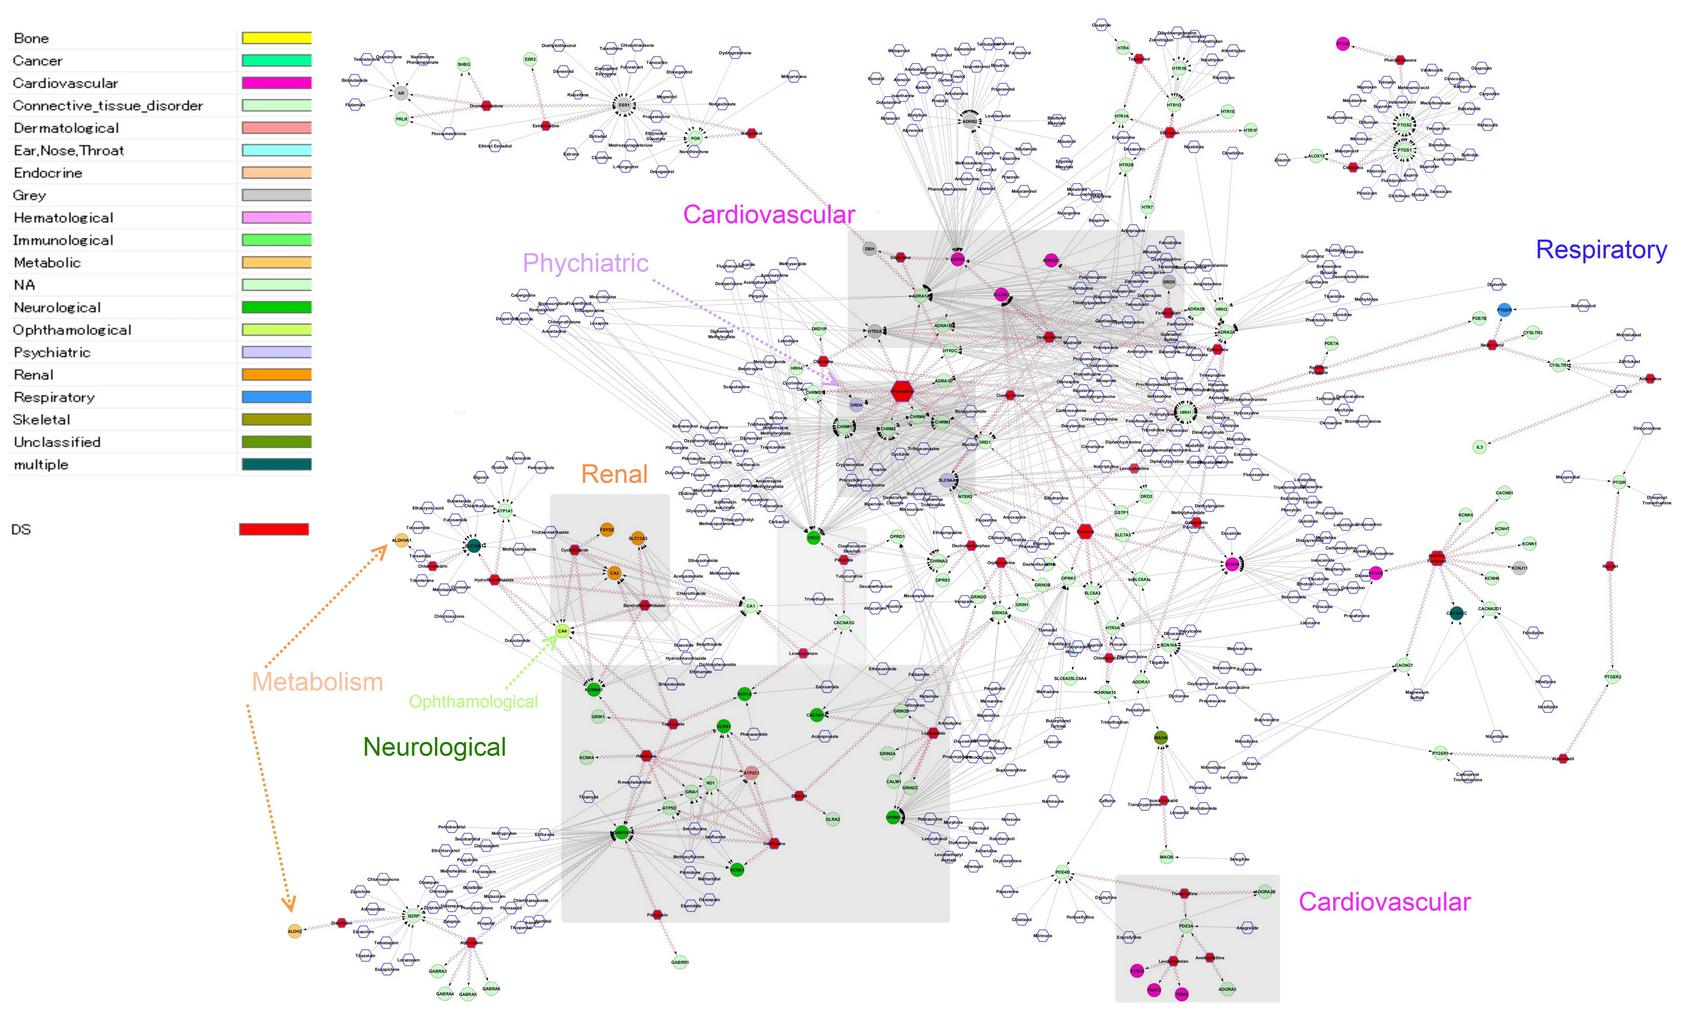
\includegraphics[scale = 0.22]{img/multi.jpg}
  \caption{Esempio di \textit{drug-target protein network}, rappresentata
    mediante \textit{grafo multipartito}.}  
  \label{fig:mbip}
\end{figure}
\newpage
Un esempio invece di rete tripartita può essere la rappresentazione di un
\textit{pathway metabolico}\footnote{Réka Albert; Scale-free networks in cell
  biology. J Cell Sci 1 November 2005; 118 (21): 4947–4957. doi:
  https://doi.org/10.1242/jcs.02714}: 
\begin{figure}[H]
  \centering
  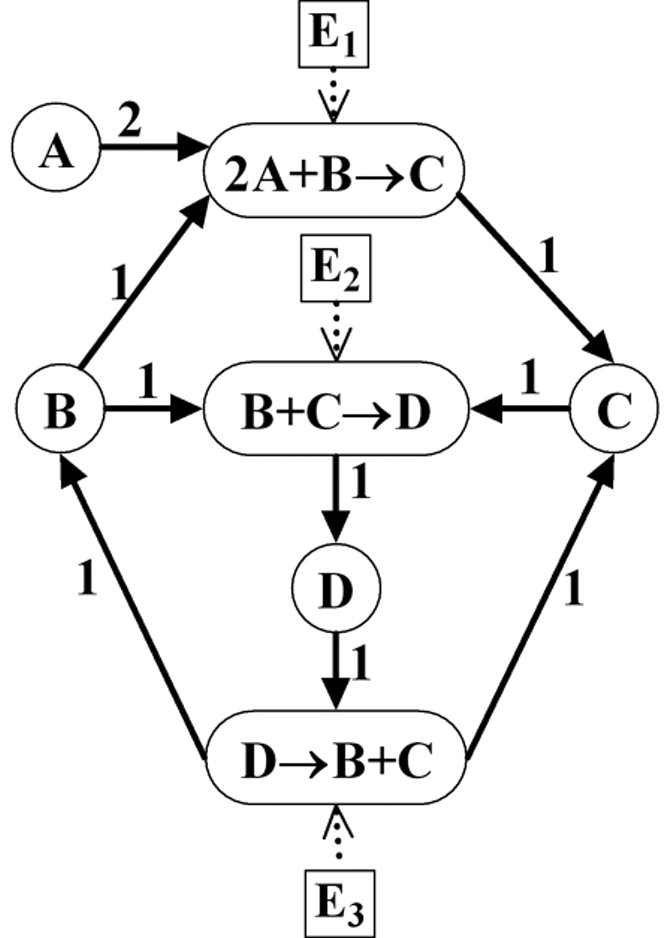
\includegraphics[scale = 0.22]{img/tri.jpg} 
\end{figure}
dove si hanno tre tipologie di nodo:
\begin{enumerate}
  \item nodi per i \textit{reagenti} (nell'immagine rappresentati da cerchi)
  \item nodi per le \textit{reazioni} (nell'immagine rappresentate da ovali)
  \item nodi per gli \textit{enzimi} (nell'immagine rappresentati da quadrati)
\end{enumerate}
Si hanno inoltre due tipologie di archi:
\begin{enumerate}
  \item le linee solide per rappresentare il \textit{mass flow},
  ovvero il \textit{tasso di turnover} delle molecole attraverso una via
  metabolica, tasso che serve ad indicare il dispendio energetico (???)
  \item le linee tratteggiate per la \textit{catalisi}, ovvero fenomeno chimico
  attraverso il quale la velocità di una reazione chimica subisce delle
  variazioni per l'intervento di una sostanza (o una miscela di sostanze) detta
  catalizzatore, che non viene consumata dal procedere della reazione
  stessa\footnote{\url{https://it.wikipedia.org/wiki/Catalisi}} 
\end{enumerate}
Inoltre i pesi degli archi indicano i \textit{coefficienti stechiometrici}, che
rappresentano infatti il rapporto tra le moli delle diverse sostanze, dei
reagenti.  \\
Ovviamente l'uso delle reti in ambito biologico può essere espanso, considerando
ad esempio i legami tra più reti, che rappresentano vari livelli, ad esempio:
\begin{itemize}
  \item \textit{reti sociali}, da usare comunque con cautela a causa della loro
  alta probabilità di portare \textit{falsi positivi/negativi} anche se possono
  rappresentare informazioni importanti. Ormai si tende comunque a preferire il
  dato del singolo paziente, puntando alla \textit{medicina personalizzata} in
  quando ``la media tra i pazienti'' raramente è un dato utile. Esse
  possono rappresentare legami 
  famigliari, vicinanza tra persone, informazioni sui luoghi in cui si vive
  etc$\ldots$ 
  \item \textit{disease networks}
  \item \textit{reti metaboliche}
  \item \textit{reti PPI}
  \item \textit{reti di regolazione genica}
  \item $\ldots$
\end{itemize}
I vari livelli sono ovviamente connessi a vicenda ma non sempre è facile
studiare tali connessioni a causa della mancanza di dati etc$\ldots$\\
Altri esempi interessanti di uso sono le \textbf{reti in ecologia}, come, ad
esempio, lo 
studio di Faust e Raes\footnote{Faust, K., Raes, J. Microbial interactions: from
  networks to models. Nat Rev Microbiol 10, 538–550
  (2012). https://doi.org/10.1038/nrmicro2832} dove si studiavano le
\textit{interazioni microbiche}, tra cui il parassitismo, il mutualismo la
competizione etc$\ldots$ tramite appunto delle reti.\\
Un uso recente delle reti è anche quello nelle \textbf{neuroscienze}, per
capire, durante una malattia, cosa non stia funzionando bene nel cervello. Un
esempio è lo studio di Chennu, Srivas et al.\footnote{Chennu, Srivas, et
  al. "Spectral 
  signatures of reorganised brain networks in disorders of consciousness." PLoS
  computational biology 10.10 (2014): e1003887.} dove si è sfruttata la
relazione tra reti e funzionalità del cervello per identificare quali aree del
cervello/funzioni del cervello funzionassero male in pazienti in stato
vegetativo e pazienti 
minimamente coscienti, facendo il paragone con vari soggetti controllo
sani. Sono stati usati anche i concetti di grado etc$\ldots$ nello studio.
\section{Tipologie di Reti}
Un aspetto fondamentale nello studio delle reti è inoltre quello che sia la
\textit{degree distribution} $P(k)$ che il \textit{average clustering
  coefficient} $C(k)$ sono \textbf{indipendenti} dalla grandezza delle rete e
possono essere usati per identificare caratteristiche generali e classificare le
reti stessi. Tra le tipologie più importanti abbiamo:
\begin{itemize}
  \item \textbf{random network}
  \item \textbf{scale-free network}
  \item \textbf{hierarchical network}
\end{itemize}
Ad ogni tipologia ovviamente corrisponde un certo insieme di caratteristiche,
come ad esempio le seguenti catalogate da Mitchell\footnote{Mitchell,
  Melanie. (2006). Field review: Complex systems: Network thinking. Artificial
  Intelligence. 170. 1194-1212. 10.1016/j.artint.2006.10.002.}:
\begin{figure}[H]
  \centering
  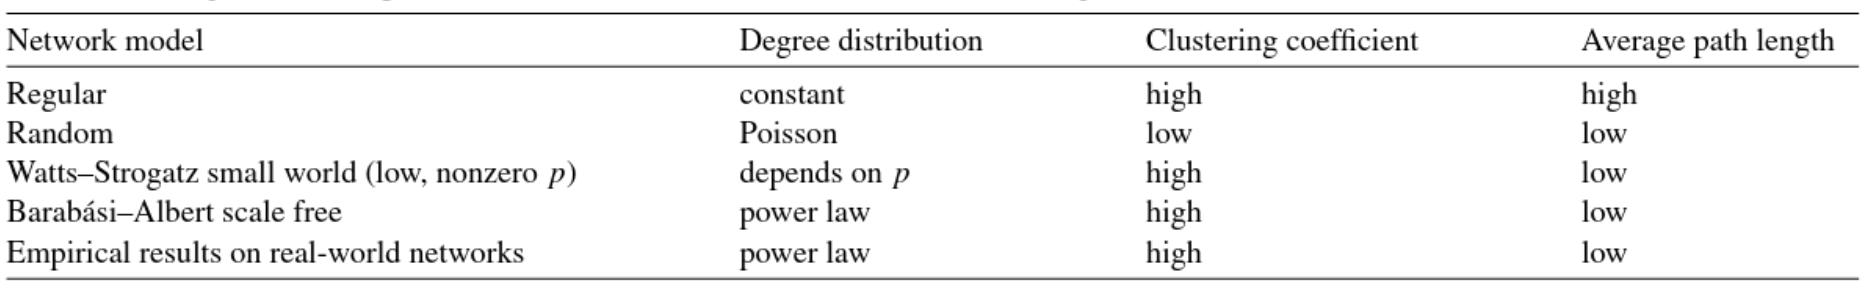
\includegraphics[width = \textwidth]{img/net.jpg} 
\end{figure}
\newpage
\subsection{Random Network}
Si comincia parlando delle \textbf{random network}, dette anche
\textbf{Erd\"{o}s-Rényi model}, dal nome di coloro che le formalizzarono nel
1960.\\
Si hanno quindi le seguenti caratteristiche principali per una \textit{random
  network}: 
\begin{itemize}
  \item la rete è \textbf{statisticamente omogenea}, infatti la maggior parte
  dei nodi ha circa lo stesso numero di archi incidenti che quindi è vicino al
  grado medio della rete $\langle k \rangle$
  \item la \textit{degree distribution} segue una \textbf{distribuzione di
    Poisson}, avendo quindi che si hanno davvero pochissimi nodi con un numero
  di archi incidenti maggiore o minore del valore medio. Si ha quindi,
  graficamente, una ``campana'' molto stretta sulla media del grado di tutti i
  nodi della rete,
  come visibile in figura \ref{fig:pois}\footnote{Réka Albert; Scale-free
    networks in cell biology. J Cell Sci 1 November 2005; 118 (21):
    4947–4957. doi: https://doi.org/10.1242/jcs.02714} 
  \item non si ha \textbf{modularità intrinseca}, non avendo quindi
  \textit{moduli} e avendo che $C(k)$è indipendente dal valore di $k$. Si hanno
  quindi pochi cluster
  \item sono caratterizzate dalla \textbf{small world property}
\end{itemize}
In merito all'ultimo punto bisogna formalizzare meglio quanto già
anticipato. Quando tale proprietà è garantita si ha che la lunghezza media di
un cammino tra due nodi è proporzionale a $\ln |V|$, assicurando quindi alta
velocità di trasmissione delle ``informazioni'' nella rete. Questo è necessario
nei sistemi biologici in quanto, per natura, si hanno sempre un numero basso di
operazioni per ridurre sia i tempi che per ottimizzare i consumi energetica. In
certi casi si ha la \textbf{ultra small world property} dove la proprietà viene
estremizzata e infatti si arriva ad avere che la lunghezza media di
un cammino tra due nodi è proporzionale a $\ln(\ln |V|)$, che è molto minore
di $\ln(|V|)$.\\
Un esempio di questa tipologia di rete è visibile in figura
\ref{fig:rnet}\footnote{Barabási, AL., Oltvai, Z. Network biology: understanding
  the cell's functional organization. Nat Rev Genet 5, 101–113
  (2004). https://doi.org/10.1038/nrg1272} 
\begin{figure}
  \centering
  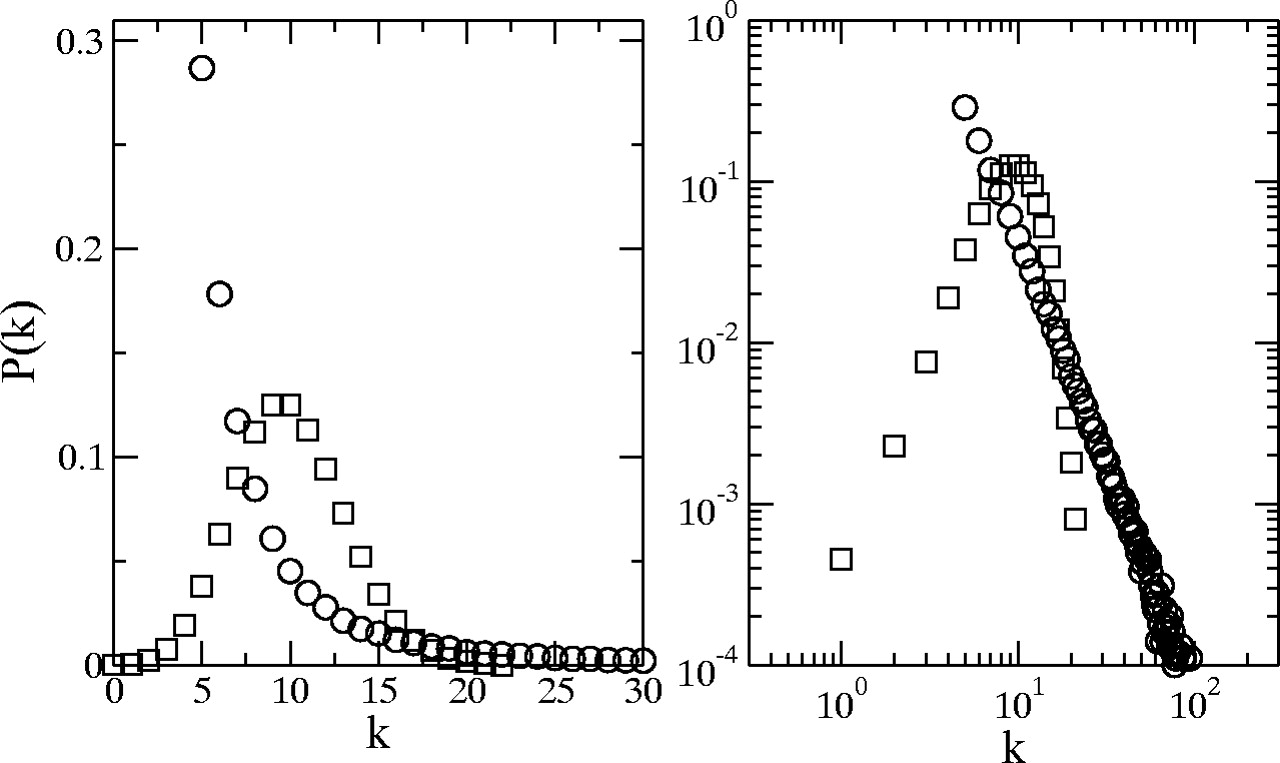
\includegraphics[scale = 0.2]{img/pois.jpeg}
  \caption{Confronto tra la \textit{distribuzione di Poisson}, rappresentata dai
    quadrati, e la \textit{power-law}, rappresentata coi cerchi, prima in scala
    normale e poi in scala logaritmica.}
  \label{fig:pois}
\end{figure}
\begin{figure}
  \centering
  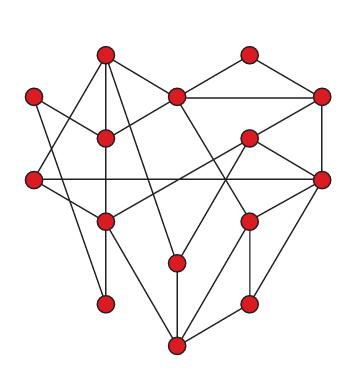
\includegraphics[scale = 2.25]{img/rnet1.jpg}\\
  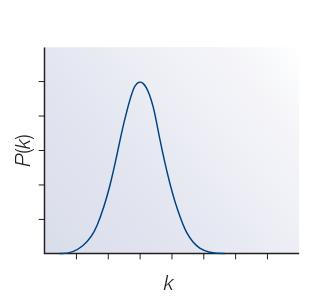
\includegraphics[scale = 1.75]{img/rnet2.jpg}
  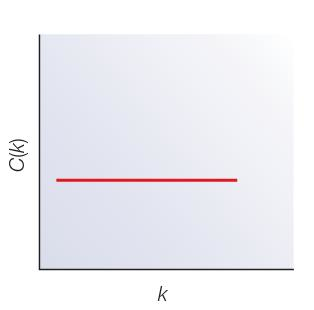
\includegraphics[scale = 1.75]{img/rnet3.jpg}
  \caption{Esempio di \textit{random network} con i grafici di $P(k)$ e $C(k)$.}
  \label{fig:rnet}
\end{figure}
\newpage
\subsection{Scale-Free Networks}
Si hanno poi le \textbf{scale-free network}, dette anche \textbf{Barabási-Albert
  model}, dal nome di coloro che le formalizzarono nel 1999.\\
Si hanno quindi le seguenti caratteristiche principali per una
\textit{scale-free network}:
\begin{itemize}
  \item la rete è \textbf{non omogenea}, da qui il nome scale-free. Si hanno
  quindi pochi nodi fortemente connessi, gli \textbf{hub}, e tanti nodi con
  pochissimi archi incidenti
  \item la \textit{degree distribution} segue la \textbf{power-law}, come
  visibile in figura \ref{fig:pois}\footnote{Réka Albert; Scale-free 
    networks in cell biology. J Cell Sci 1 November 2005; 118 (21):
    4947–4957. doi: https://doi.org/10.1242/jcs.02714}, avendo che: 
  \[P(k)=k^{-\gamma},\,\,\gamma\in\mathbb{R}\]
  dove si ha la \textit{ultra small world property} per $2<\gamma<3$, anche se
  in realtà dei valori di $\gamma$ che eccedono questo range comportano altre
  tipologie di rete
  \item non si ha \textbf{modularità intrinseca}, non avendo quindi moduli e
  avendo che $C(k)$ è indipendente dal valore di $k$. Si hanno quindi pochi
  cluster 
\end{itemize}
Nel dettaglio, al variare di $\gamma$, dato $\langle d\rangle$ come lunghezza
del cammino medio e $k_{\max}\sim N^{\frac{1}{\gamma -1}}$:
\begin{itemize}
  \item se $\gamma<2$ si parla di \textbf{reti anomale}, avendo
  $\langle k\rangle$ che diverge e $\langle k^2\rangle$ che diverge. Si ha in
  questo caso che $\langle d\rangle$ è circa costante. Non si hanno
  \textit{large network} per tali valori di $\gamma$
  \item se $\gamma = 2$ non si ha una categorizzazione ma si avrebbe
  $k_{\max}\sim N$ 
  \item se $2<\gamma<3$ si parla quindi di \textbf{scale-free network}, avendo
  $\langle k\rangle$ finito e $\langle k^2\rangle$ che diverge. Si ha in
  questo caso che $\langle d\rangle\sim\ln(\ln(N))$ parlando di \textit{ultra
    small world}
  \item se $\gamma = 3$ si ha un \textit{punto critico} ma si ha $\langle
  d\rangle\sim\frac{\ln N}{\ln(\ln(N))}$
  \item se $\gamma>3$ si parla di reti indistinguibili da una \textbf{random
    network} (come le \textit{reti di citazioni}, \textit{reti di
    collaborazioni} etc$\ldots$), avendo 
  $\langle k\rangle$ finito e $\langle k^2\rangle$ che finito. Si ha in
  questo caso che $\langle d\rangle\sim\frac{\ln N}{\ln\langle k\rangle}$
  parlando di \textit{small world} 
\end{itemize}
Questa tipologia di rete è solitamente quella più usata in ambito
biologico, infatti possiamo ad esempio pensare ad una proteina come
\textit{p53}, tra le principali responsabili dell'\textit{apoptosi}, che in una
rete sarà sicuramente un \textit{hub}. Altri esempi possono essere le molecole
di \textit{ATP}, \textit{ADP} etc$\ldots$. Alcuni esempi sono (\textit{alcune
  immagine relative sono presenti sulle slide}): 
\begin{itemize}
  \item \textit{rete PPI per il lievito}
  \item \textit{rete di proteine per c. elegans, un eucariote}
  \item \textit{reti metaboliche per a. fulgidus, un archaea, e. coli, un
    batterio, c. elegans etc$\ldots$}, dove le reti sono modellate da grafi
  orientati e si ha che sia la \textit{indegree distribution} che la
  \textit{outdegree distribution} seguono la \textit{power-law}
\end{itemize}
Ma si hanno anche esempi non biologici come:
\begin{itemize}
  \item \textit{world wide web}
  \item \textit{connessioni tra gli aeroporti mondiali}
\end{itemize}
Interessante è cercare di capire perché i sistemi biologici tendono a comportare
\textit{scale-free network}. Si suppone infatti che tale comportamento abbia
due cause principali:
\begin{enumerate}
  \item la \textbf{crescita (\textit{growth})}
  \item il cosiddetto \textbf{attaccamento preferenziale (\textit{preferential
      attachment})} 
\end{enumerate}
Infatti questi due processi generano \textit{hub} tramite il processo detto
\textit{``rich-gets-richer''} per il quale nuovi nodi tendono a collegarsi a
nodi con un grado alto, facendo sì che i nodi con alto grado siano destinati ad
avere sempre più nodi incidenti, aumentandone ancora il grado e aumentando la
possibilità che nuovi nodi vengano attaccati a loro. Si ha inoltre che è molto
probabile che i primi nodi della rete siano quelli destinati ad avere un grado
alto che cresce all'aggiunta di nuovi nodi (cosa che porta ad avere reti
dominate da \textit{hub}). Questo comportamento è anche alla base
dell'\textit{algoritmo di PageRank}. \\
Quindi in generale si hanno varie ipotesi possibili:
\begin{itemize}
  \item l'\textit{evoluzione}
  \item \textit{ottimizzazione energetica}
  \item maggior \textit{robustezza} (concetto che si introdurrà a breve) nei
  confronti delle perturbazioni 
\end{itemize}
Un'altra teoria molto accreditata è quella, parlando di \textit{reti PPI},
rileva le origini di tali reti nella \textbf{duplicazione genica}, spiegata
visivamente in figura \ref{fig:dup}\footnote{Barabási, AL., Oltvai, Z. Network
  biology: understanding the cell's functional organization. Nat Rev Genet 5,
  101–113 (2004). https://doi.org/10.1038/nrg1272}. Quando le 
cellule si dividono, uno o più geni potrebbero essere copiati due volte nel
genoma della prole e ciò induce la crescita nella \textit{rete PPI} poiché
esiste un gene in più che codifica per una nuova proteina, avendo letteralmente
un nodo in più uguale ad un altro. La nuova proteina ha la stessa struttura
della vecchia, quindi entrambe interagiscono con le stesse proteine e le
proteine che hanno interagito con la proteina duplicata originale acquisiranno
ciascuna una nuova interazione con la nuova proteina. Inoltre le proteine con un
gran numero di interazioni tendono a ottenere collegamenti più spesso, poiché è
più probabile che interagiscano con la proteina che è stata
duplicata. Si creano così \textit{hub} e \textit{scale-free network}. Ovviamente
poi, nella realtà, tali proteine duplicate è difficile che 
restino esattamente uguali e in ogni caso non è un discorso semplice pensare di
rimuovere a priori tali nodi dalla rete.\\
\begin{figure}
  \centering
  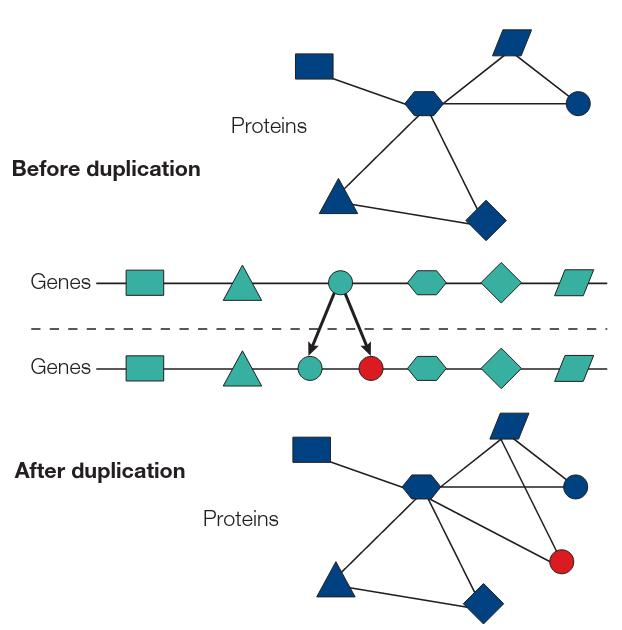
\includegraphics[scale = 1.5]{img/dup.jpg}
  \caption{Rappresentazione grafica dell'ipotetico processo di
    \textit{duplicazione genica}, che produce i due nodi rappresentati da
    cerchi, che porterebbe a \textit{scale-free network}.}  
  \label{fig:dup}
\end{figure}
Tali modelli trovano molto spazio anche fuori dal mondo biologico, basti
pensare a reti per modellare materiali etc$\ldots$\\
Un esempio di questa tipologia di rete è visibile in figura
\ref{fig:sfnet}\footnote{Barabási, AL., Oltvai, Z. Network biology: understanding
  the cell's functional organization. Nat Rev Genet 5, 101–113
  (2004). https://doi.org/10.1038/nrg1272}.
\begin{figure}
  \centering
  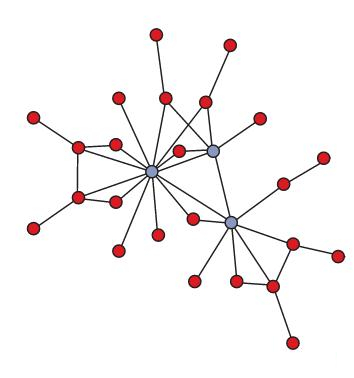
\includegraphics[scale = 2.25]{img/sfnet1.jpg}\\
  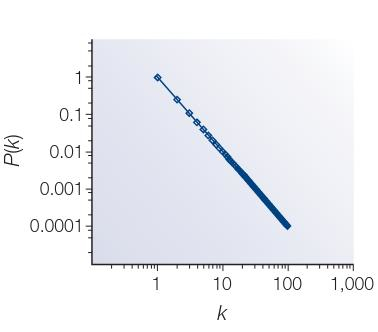
\includegraphics[scale = 1.75]{img/sfnet2.jpg}
  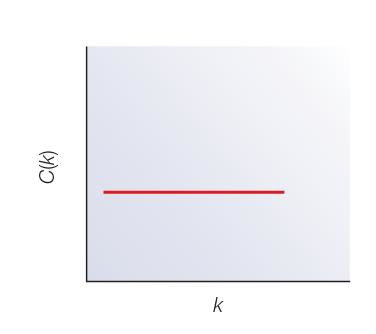
\includegraphics[scale = 1.75]{img/sfnet3.jpg}
  \caption{Esempio di \textit{scale-free network} con i grafici di $P(k)$ e
    $C(k)$. Gli \textit{hub} sono colorati in grigio.} 
  \label{fig:sfnet}
\end{figure}
\subsubsection{Robustezza Topologica}
Un altro discorso interessante da introdurre in questo contesto è quello della
``resistenza'' da parte delle \textit{scale-free} network alle
\textit{perturbazioni}. Si parla quindi di \textbf{robustezza topologica} delle
reti. 
\begin{definizione}
  Si definisce \textbf{robustezza} come l'abilità del sistema di rispondere a
  cambiamenti nelle condizioni esterne o nell'organizzazione interna, mantenendo
  un comportamento ``normale''.
\end{definizione}
Una formalizzazione matematica di un ``punteggio'' relativo alla robustezza non
è discorso banale e nemmeno unico. Si possono avere varie strategie basate sul
numero di \textit{hub}, sui pesi degli archi, sulle caratteristiche globali
della rete etc$\ldots$\\
Ci si chiede quindi:
\begin{itemize}
  \item cosa succede se si disabilita/elimina un numero sostanziale di nodi in
  una rete? 
  \item cosa succede se si verifica un errore accidentale?
  \item cosa succede se si rimuovono deliberatamente nodi specifici nella rete? 
\end{itemize}
Parlando di rimozione di nodi potrei avere infatti due casi:
\begin{enumerate}
  \item un \textbf{random attack}, dove letteralmente il nodo da eliminare è uno
  casuale e, avendo molti più nodi con basso grado che \textit{hub} (che sono
  pochissimi), si ha che la rete ``collassa'' ad un grafo sconnesso molto
  lentamente in quanto gli \textit{hub} impiegano diverse rimozioni di nodi a
  sparire 
  \item un \textbf{deliberate attack} sugli \textit{hub}, dove appunto si mira
  ad eliminare specificamente i nodi \textit{hub}. In questo caso la rete
  ``collassa'' ad un grafo sconnesso molto in fretta
\end{enumerate}
Le chance di poter studiare \textit{proprietà emergenti} da una rete è
direttamente correlata alla ``resistenza'' ai vari tipi di attacchi anche se
bisogna ricordare che non sempre avere \textit{hub} è a priori la situazione
migliore per uno studio.
\subsection{Hierarchical Networks}
Vediamo infine l'ultima tipologia di rete tratta in questo corso, le
\textbf{hierarchical networks}. Tali reti hanno comunque poco spazio nella
\textit{systems biology}.\\
Si hanno quindi le seguenti caratteristiche principali:
\begin{itemize}
  \item si ha la \textit{coesistenza} di \textbf{modularità}, \textbf{clustering
    locale} e \textbf{topologia scale-free}. Si hanno quindi cluster, poco
  collegati tra loro, con all'interno \textit{modules}
  \item la \textit{degree distribution} segue la \textbf{power-law}, come
  visibile in figura \ref{fig:pois}\footnote{Réka Albert; Scale-free 
    networks in cell biology. J Cell Sci 1 November 2005; 118 (21):
    4947–4957. doi: https://doi.org/10.1242/jcs.02714}
  \item si ha \textbf{modularità intrinseca}, avendo che $C(k)$ è proporzionale
  a $\frac{1}{k}$
\end{itemize}
Prove crescenti suggeriscono che le reti biologiche contengono piccoli
sottografi conservati dai processi evolutivi che hanno una struttura ben
definita. Possiamo quindi caratterizzarli, anche se è già stato fatto, in modo
descrittivo in quanto non esiste una vera e propria formalizzazione matematica
di essi: 
\begin{itemize}
  \item i \textbf{module}, ovvero un gruppo di nodi collegati fisicamente o
  funzionalmente che lavorano insieme per ottenere una specifica funzione
  cellulare, come ad esempio la trasduzione del segnale di una determinata
  molecola 
  \item i \textbf{motif}, ovvero sottografi che si verificano significativamente
  più frequentemente nella rete data di quanto si otterrebbe con una
  \textit{random network}
\end{itemize}
Questi due tipi di sottografo sono essenziali negli studi in \textit{systems
  biology} tramite reti ma la loro identificazione è un problema
computazionalmente complesso, oltre ad essere, come detto, non ben definito. \\
Parlando di \textit{motif} se ne possono identificare varie tipologie, come
quelle proposte da Albert\footnote{Réka Albert; Scale-free networks in cell
  biology. J Cell Sci 1 November 2005; 118 (21): 4947–4957. doi:
  https://doi.org/10.1242/jcs.02714}:
\begin{itemize}
  \item \textbf{transcriptional feed-forward loop}, ad esempio:
  \begin{figure}[H]
    \centering
    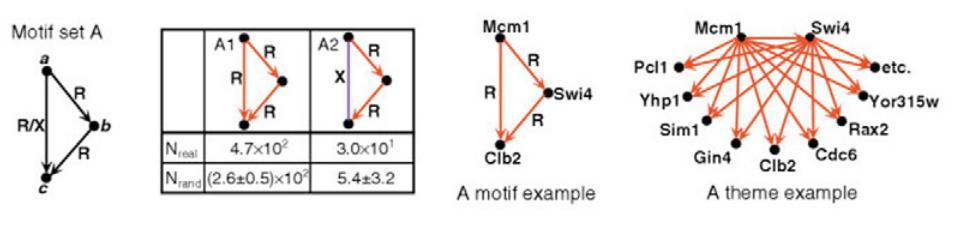
\includegraphics[width = \textwidth]{img/mot1.jpg}
  \end{figure}
  dove con $R$ si identificano gli archi per le regolazioni trascrizionali e con
  $X$ le \textit{espressioni correlate}
  \item \textbf{transcriptional co-regulation}, ad esempio:
  \begin{figure}[H]
    \centering
    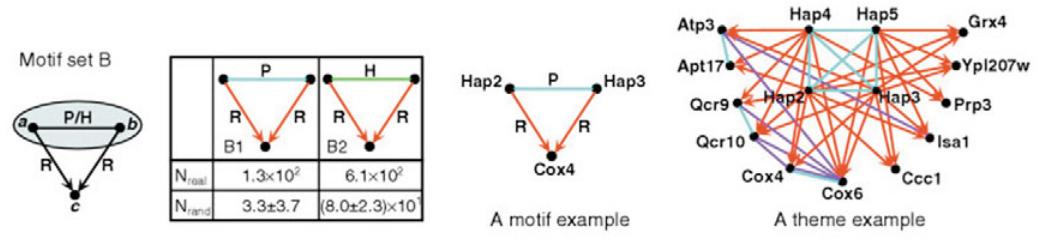
\includegraphics[width = \textwidth]{img/mot2.jpg}
  \end{figure}
  dove con $R$ si identificano gli archi per le \textit{regolazioni
    trascrizionali}, con 
  $P$ le \textit{interazioni proteiche} e con $H$ l'\textit{omologia tra
    sequenze} 
  \item \textbf{co-regulation of members of a protein complex}, ad esempio:
  \begin{figure}[H]
    \centering
    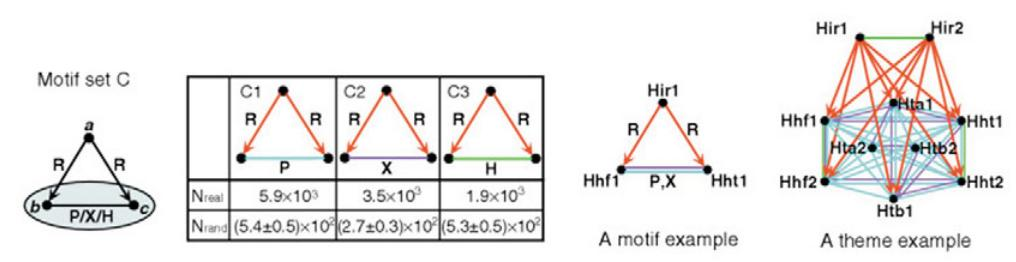
\includegraphics[width = \textwidth]{img/mot3.jpg}
  \end{figure}
  dove con $R$ si identificano gli archi per le \textit{regolazioni
    trascrizionali}, con 
  $P$ le \textit{interazioni proteiche}, con $H$ l'\textit{omologia tra
    sequenze} e con
  $X$ le \textit{espressioni correlate}
  \item \textbf{co-expressed protein cliques}, ad esempio:
  \begin{figure}[H]
    \centering
    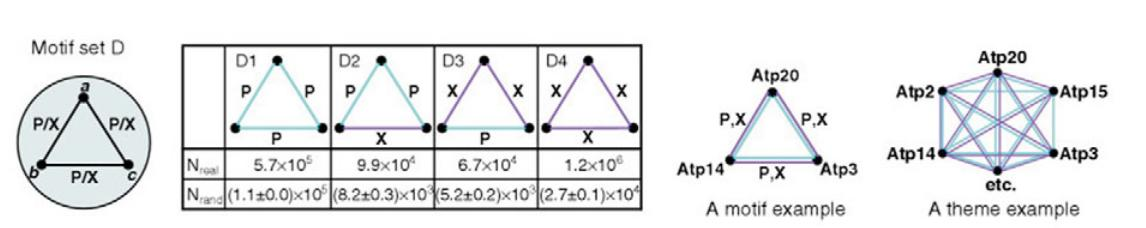
\includegraphics[width = \textwidth]{img/mot4.jpg}
  \end{figure}
  dove $P$ le \textit{interazioni proteiche} con
  $X$ le \textit{espressioni correlate}
\end{itemize}
Un esempio di questa tipologia di rete è visibile in figura
\ref{fig:sfnet2}\footnote{Barabási, AL., Oltvai, Z. Network biology: understanding
  the cell's functional organization. Nat Rev Genet 5, 101–113
  (2004). https://doi.org/10.1038/nrg1272}.
\begin{figure}
  \centering
  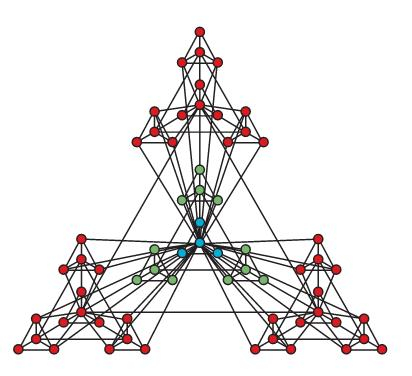
\includegraphics[scale = 2.25]{img/hnet1.jpg}\\
  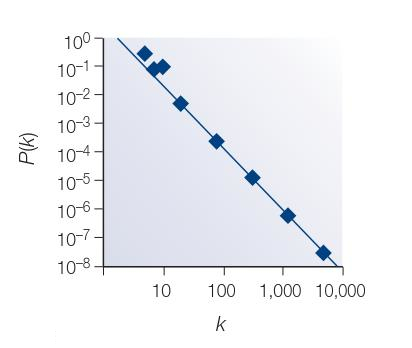
\includegraphics[scale = 1.75]{img/hnet2.jpg}
  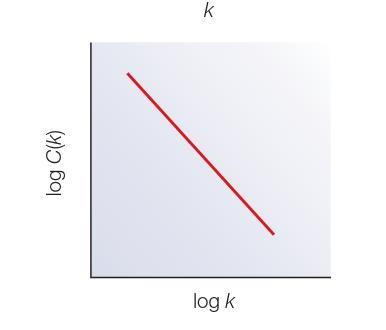
\includegraphics[scale = 1.75]{img/hnet3.jpg}
  \caption{Esempio di \textit{hierarchical network} con i grafici di $P(k)$ e
    $C(k)$. Gli \textit{hub} sono colorati in grigio.} 
  \label{fig:sfnet2}
\end{figure}
\textbf{Un testo online interessante sul tema delle reti si trova al link:\\}
\begin{center}
  \url{http://networksciencebook.com}
\end{center}
\section{Software}
Per analizzare reti, biologiche ma anche non biologiche (si passa anche a studi
di scienze sociali e reti complesse generiche), uno dei tool standard
in uso è \textbf{Cytoscape}\footnote{Cline, Melissa S et al. “Integration of
  biological networks and gene expression data using Cytoscape.” Nature
  protocols vol. 2,10 (2007): 2366-82. doi:10.1038/nprot.2007.324}, disponibile
gratuitamente a 
\url{http://www.cytoscape.org/}.\\
Citando direttamente:
\begin{center}
  \textit{``Cytoscape is an open source software platform for visualizing
    molecular 
    interaction networks and biological pathways and integrating these networks
    with annotations, gene expression profiles and other state data.''\\
    ...\\
    ``Although Cytoscape was originally designed for biological research, now it
    is a 
    general platform for complex network analysis and visualization.''\\
    ...\\
    ``Cytoscape core distribution provides a basic set of features for data
    integration, 
    analysis, and visualization. Additional features are available as Apps
    (formerly called 
    Plugins). Apps are available for network and molecular profiling analyses,
    new layouts, additional file format support, scripting, and connection with
    databases.''  } 
\end{center}
Come scritto si hanno a disposizione una vasta serie di plugins, detti
\textit{apps} e ben introdotti dal paper di Saito et al.\footnote{Saito R, Smoot
ME, Ono K, et al. A travel guide to Cytoscape plugins. Nat
Methods. 2012;9(11):1069-1076. doi:10.1038/nmeth.2212}, che aggiungono
moltissime funzionalità, tra cui, ad esempio, 
collegare una rete ad un database esterno per fare \textit{gene enrichment}. 
\chapter{Logic-Based Modelling}
Si introducono ora i \textbf{modelli logic-based}.\\
Ricordiamo che tali modelli, come visibile in figura \ref{fig:appro}:
\begin{itemize}
  \item sono sistemi meno \textit{large-scale} di quanto lo fossero i
  \textit{modelli interaction-based}
  \item presentano tendenzialmente un basso costo computazionale
  \item presentano un livello di dettaglio, per quanto ambiguo nello schema,
  variabile
  \item presentano alcune difficoltà nella misurazione dei dati
\end{itemize}
Il tutto comporta una miglior capacità predittiva rispetto ai \textit{modelli
  interaction-based} e, grazie all'uso di vari tipi di logiche, può portare
anche a ottenere modelli molto più predittivi.\\
Un'altra differenza sostanziale rispetto ai \textit{modelli interaction-based} è
che si può iniziare a parlare di \textit{simulazioni}, superando il ``limite''
delle sole analisi. In questo caso i modelli più semplici si basano sulla
\textit{logica booleana} e, come si vedrà, se simulazioni e le analisi
consistono nel determinare:
\begin{itemize}
  \item \textbf{cicli}, ovvero sequenze ripetute di stati di sistema
  \item \textbf{attrattori}, ovvero stati finali raggiungibili da un qualsiasi
  stato iniziale
  \item \textbf{bacini di attrazione}, percorsi di stati intermedi che iniziano
  da uno stato iniziale e terminano in un attrattore
\end{itemize}
Con l'aggiunta della \textbf{logica fuzzy}, più complessa di quella booleana, si
può anche derivare il \textit{comportamento dinamico} del sistema, ad esempio
derivando la variazione temporale del valore di ogni componente in uno o più
stati, magari dopo una certa \textit{perturbazione}. Si parla quindi di
\textbf{modelli qualitativi} e 
\textbf{dinamici}. L'informazione \textit{quantitativa} è ridotta al minimo, non
avendo la rappresentazione di vere e proprie interazioni/proprietà chimiche e
fisiche 
come, ad esempio, la rappresentazione di \textit{kinetic-rate} etc$\ldots$\\ 
Come detto si hanno sia \textit{sistemi small-scale} che \textit{sistemi
  large-scale}, anche se comunque di dimensioni ridotte rispetto ai
\textit{modelli interaction-based}, e ad esempio sono usati per:
\begin{itemize}
  \item \textbf{reti di regolazione gene-gene}
  \item \textbf{pathway per il segnale di trasduzione}
  \item \textbf{differenziazione cellulare}, soprattutto grazie allo studio
  degli \textit{attrattori}
  \item \textbf{pathway per la morte programmata cellulare}
\end{itemize}
Tecnologie sperimentali di natura qualitativa (ad esempio \textit{targeting
  genico} e \textit{screening fenotipici}) hanno portato allo sviluppo di metodi
computazionali per modellare e analizzare reti regolatorie geniche sulla base di
regole logiche. L'architettura di tali modelli, per semplificare, consiste in
due ``aspetti'' principali:
\begin{enumerate}
  \item la \textbf{struttura della rete}, modellata tramite \textit{grafi
    diretti}, dove con la direzione si specificano principalmente, ma non solo,
  fenomeni di regolazione
  \item le \textbf{dinamiche della rete}, modellati tramite stati logic-based
  mutevoli e funzioni di update degli stati stessi, che garantiscono
  un'evoluzione nel tempo
\end{enumerate}
L'idea generale è quindi quella di partire da uno \textbf{stato iniziale} per
poi assegnare un nuovo valore ad ogni variabile del modello, quindi ad ogni nodo
della rete, tramite l'uso di \textit{funzioni logiche} che combinano i valori
delle variabili dello stato corrente per produrre il nuovo stato.\\
Interessante è elencare fin da subito alcuni \textbf{pro} di questo approccio
modellistico:
\begin{itemize}
  \item i \textit{modelli logic-based} sono \textbf{versatili}, in quanto una
  variabile può praticamente rappresentare qualsiasi cosa, come ad esempio un
  gene, un'attività genica, la presenza di una proteina, un fenotipo, lo stato
  di una cellula etc$\ldots$ Inoltre si possono mischiare componenti eterogenee
  in modo abbastanza semplice, a differenza di quanto accadeva coi
  \textit{modelli interaction-based}, dove era molto più complesso fare ciò
  \item i \textit{modelli logic-based} sono \textbf{flessibili}, in quanto lo
  stato di un dato componente cellulare può essere rappresentato da una o più
  variabili, con diversi insiemi di valori. Quindi una certa componente può
  avere funzioni diverse a seconda dello stato del sistema e questo risolve
  quanto visto nel caso dei \textit{modelli interaction-based} in merito ai
  nodi ripetuti nella rete, avendo che in questo caso i due o più nodi sono
  ben distinti, magari avendo un nodo per una certa proteina e un altro per la
  stessa proteina ma fosforilata (si ricorda che la \textit{fosforilazione} è
  una reazione chimica, fondamentale in biochimica,  che consiste
  nell'addizione di un gruppo fosfato, $PO_4^{3-}$, ad una proteina o ad
  un'altra molecola e si ricorda che gli enzimi che solitamente catalizzano le
  fosforilazioni sono le chinasi)   
  \item gli effetti delle \textit{perturbazioni}, come \textit{inibizioni} o
  \textit{mutazioni}, possono essere ``testati'' in modo molto facile e diretto
\end{itemize}
Si hanno però anche vari \textbf{contro}, che principalmente si riconducono al
fatto che non sono modelli meccanicistici. Infatti, per quanto si abbia alla
base un \textit{grafo diretto}, non è possibile inferire la proprietà
meccanicistica che si ha dietro la regolazione positiva/negativa, o altro, che
viene rappresentata mediante l'arco diretto. Ipotizziamo anche solo di avere due
nodi $A$ e $B$, con $A$ che regola $B$:
\begin{center}
  \begin{tikzpicture}[shorten >=1pt,node distance=2cm,on grid,auto]
    \node[state] (q_0) {$A$};
    \node[state] (q_1) [right=of q_0] {$B$};
    \path[->]
    (q_0) edge  node {} (q_1);
  \end{tikzpicture}
\end{center}
Potremmo dire che ``l'attività di $A$ stimola l'attività di $B$'' e si può
modellare una regolazione positiva o negativa ma non
potremo mai caratterizzare nel dettaglio il meccanismo stesso, che potrebbe
essere, ad esempio: 
\begin{itemize}
  \item l'attivazione della produzione di $B$
  \item l'inibizione della degradazione di $B$
  \item la stabilizzazione dell'\textit{high-activity state} di $B$
  \item $\ldots$
\end{itemize}
Posso solo sapere che c'è uno stimolo, avendo infatti perdita d'informazione che
impedisce l'inferenza dei meccanicismi. \\
Nei paragrafi precedenti si sono nominate spesso le
\textit{variabili}. Approfondendo il discorso si ha che in modello matematico
esse possono essere:
\begin{itemize}
  \item \textbf{valori booleani}, ovvero valori binari come 0/1,
  presente/assente, attivo/inattivo etc$\ldots$
  \item \textbf{valori multi-stato}, sia \textbf{linguistici} che
  \textbf{numerici}, come ad esempio nullo/basso/medio/alto, 0/1/2/3 etc$\ldots$
  \item \textbf{valori numerici interi o reali}, usati ad esempio per
  rappresentare la concentrazione o il numero di molecole
\end{itemize}
Le prime due categorie sono quindi sono a \textit{valori discreti} mentre la
terza è a \textit{valori continui}. Una categorizzazione più precisa, parlando
di \textit{modelli-logic based} si può osservare in figura
\ref{fig:log2}\footnote{Morris MK, Saez-Rodriguez J, Sorger PK, Lauffenburger
  DA. Logic-based models for the analysis of cell signaling
  networks. Biochemistry. 2010;49(15):3216-3224. doi:10.1021/bi902202q}. \\ 
È stato anche citato il cosiddetto \textit{stato iniziale del sistema}, ovvero
la \textit{condizione iniziale} del modello, che prevede l'assegnamento di un
valore, all'inizio della simulazione, ad ogni variabile del sistema. La
\textit{condizione iniziale} influisce ovviamente i risultati stessi della
simulazione, determinando come evolve il sistema nel tempo, soprattutto se si ha
una simulazione deterministica.
\begin{figure}
  \centering
  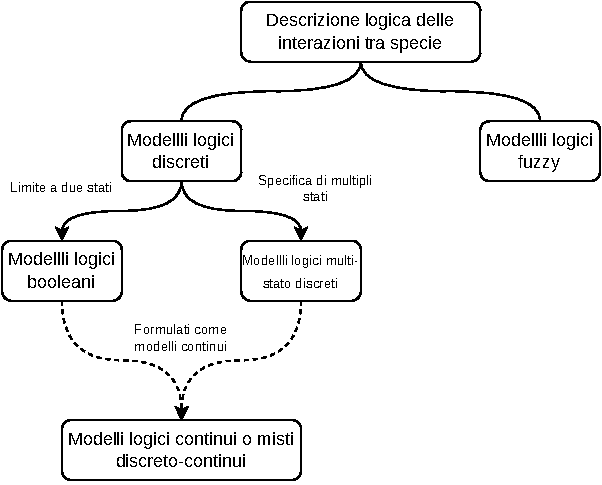
\includegraphics[scale = 1]{img/log.pdf}
  \caption{Schema riassuntivo dell'uso delle variabili in modelli
    \textit{logic-based}.}
  \label{fig:log2}
\end{figure}
\newpage
\noindent
Ovviamente la scelta tra discreto e continuo comporta delle
conseguenze. Prendiamo ad esempio la seguente situazione:
\begin{center}
  \begin{tikzpicture}[shorten >=1pt,node distance=2cm,on grid,auto]
    \node[state] (q_0) {$Y$};
    \node[state] (q_1) [right=of q_0] {$X$};
    \path[->]
    (q_0) edge  node {} (q_1);
  \end{tikzpicture}
\end{center}
e il seguente grafico\footnote{Albert, Reka, and
  Juilee Thakar. "Boolean modeling: a logic‐based dynamic approach for
  understanding signaling and regulatory networks and for making useful
  predictions." Wiley Interdisciplinary Reviews: Systems Biology and Medicine
  6.5 (2014): 353-369.}, che descrive la regolazione positiva di $Y$ su $X$: 
\begin{figure}[H]
  \centering
  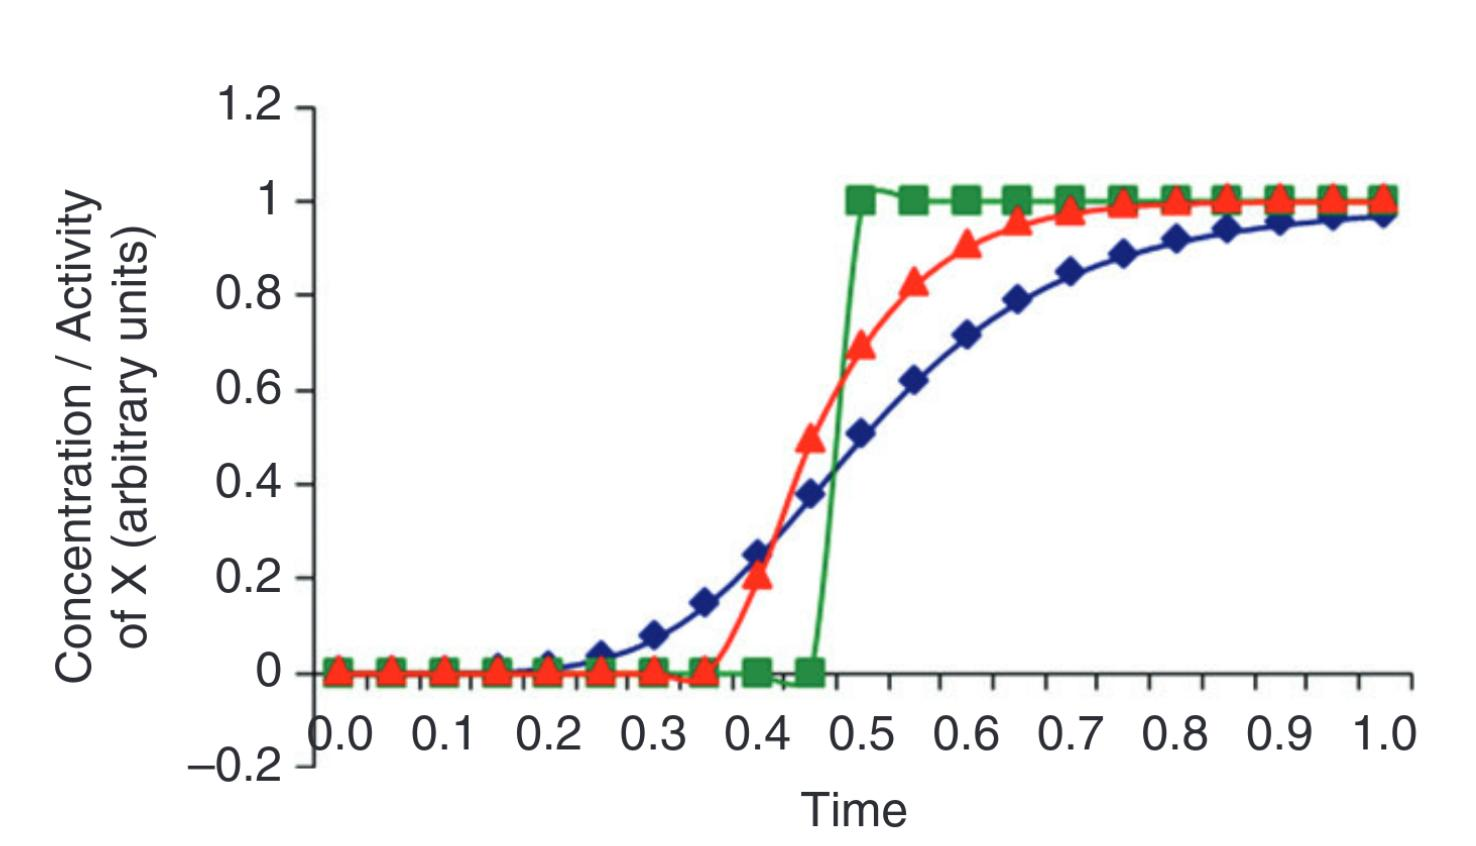
\includegraphics[scale = 0.2]{img/boolf.jpg}
\end{figure}
Nel grafico si hanno:
\begin{itemize}
  \item sull'asse delle ascisse il tempo
  \item sull'asse delle ordinate la concentrazione del nodo $X$ (si assume che
  la concentrazione/attività del nodo $Y$ cresca linearmente)
  \item la funzione booleana in verde
  \item due funzioni continue in rosso e blu che rappresentano il ``caso reale''
\end{itemize}
Si nota come il ``cambio'' per la funzione booleana sia ``secco'', prima 0 e poi
1, un certo momento temporale. Questa eccessiva semplificazione non sempre è
accettabile per descrivere casi reali ma ci sono situazioni in cui è comunque
accettabile. Potrei avere anche altre funzioni, magari multi-stato, come quelle
in figura \ref{fig:funbool}\footnote{Morris MK, Saez-Rodriguez J, Sorger PK,
  Lauffenburger DA. Logic-based models for the analysis of cell signaling 
  networks. Biochemistry. 2010;49(15):3216-3224. doi:10.1021/bi902202q}
\begin{figure}
  \centering
  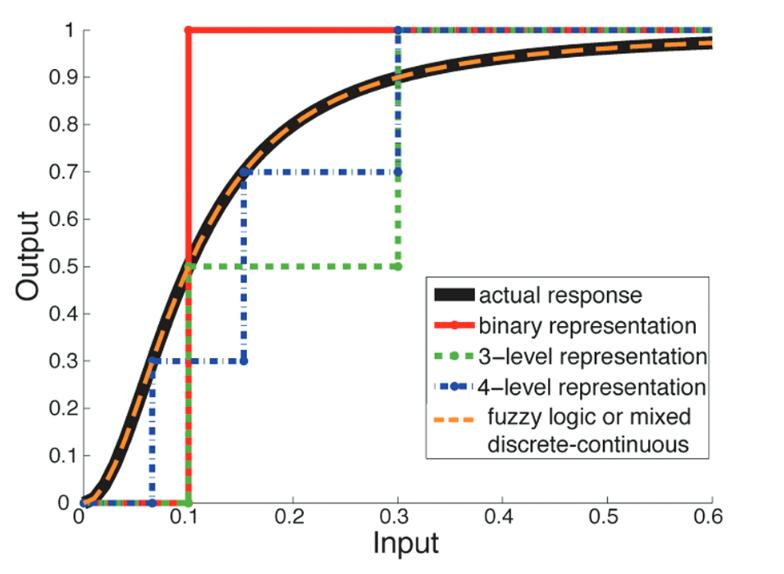
\includegraphics[scale = 0.35]{img/funbool.jpg}
  \caption{Esempio di approssimazioni di un certo andamento, partendo
    dall'approssimazione  booleana a
    quella nel caso continuo, che rappresenta correttamente la relazione
    a sigmoide tra i livelli di input e output ad esempio nel casi dell'azione
    della chinasi su un substrato, passando per diverse approssimazioni
    multi-strato.}  
  \label{fig:funbool}
\end{figure}
Si può quindi rilevare un ulteriore \textbf{contro} che si può avere in
\textit{sistemi logic-based} in quanto quando un nodo è ``off'', ad esempio, non
significa esattamente che la molecola ha zero concentrazione in quel momento nel
sistema. Si sottintende una \textit{soglia implicita} che stabilisce ``on''  e
``off'', quindi è ``off'' sse la molecola non è presente in modo
sufficiente al punto da permettere cambiamenti nelle molecole regolate da
essa. Quando supera quella soglie diventa ``on'' (ad esempio si può pensare di
avere $0\leq x\leq 1$ e che fino a $x=0.8$ si ha lo stato ``off'' e con $x>0.8$
lo stato ``on''). Si ha quindi solo
un'approssimazione qualitativa della regolazione molecolare anche se bisogna
notare che noti che molti dati sperimentali disponibili sulle regolazioni
molecolari sono di natura qualitativa. \\
Si possono, come anticipato, fare delle \textit{simulazioni} e l'aggiornamento
degli stati può essere determinato in vari modi, tramite diverse concezioni del \textit{tempo}:
\begin{itemize}
  \item tramite \textbf{iterazioni} che non rappresentano necessariamente una
  durata temporale fisica specifica, infatti un ``passo temporale'', un
  \textit{time step} può rappresentare una durata diversa per iterazioni diverse
  (magari in un caso è un evento che avviene in un secondo e in un altro che
  avviene in un'ora ma entrambi sono un singolo \textit{time step} di ugual
  durata). Si hanno inoltro due ulteriori sotto casistiche:
  \begin{enumerate}
    \item la \textbf{modalità di aggiornamento sincrona}, dove il valore di
    tutte le variabili viene ricalcolato dopo ogni singola
    iterazione. \textit{Questa sarà la modalità che verrà approfondita nel
      corso}  
    \item la \textbf{modalità di aggiornamento asincrona}, dove le variabili
    subiscono transizioni una alla volta e le variabili da aggiornare vengono
    scelte in modo tendenzialmente causale
  \end{enumerate}
  \item tramite \textbf{step discreti}, che quindi hanno una specifica durata
  eventualmente diversa l'uno dagli altri, dopo i quali avvengono gli
  aggiornamenti delle variabili
  \item tramite \textbf{tempo continuo}, dove si simula (eventualmente su una
  scala diversa) il trascorrere reale del tempo
\end{itemize}
Un'altra problematica che si presenta dopo aver capito come viene aggiornato lo
stato del sistema in un \textit{modello logic-based} è quello che il numero di
stati cresce in modo esponenziale rispetto al numero di variabili, quindi al
numero di nodi $|V|$. Questo aspetto rende complicata anche la validazione dei
modelli, validazioni che solitamente vengono fatte in modo probabilistico
(\textit{aspetto non ben chiarito a lezione ma magari si vedrà più avanti nel
  corso}). Inoltre, avendo nei \textit{modelli logic-based} solitamente l'uso di
iterazioni per descrivere l'evoluzione temporale si ha difficoltà a tracciare
processi lenti/veloci o anche \textit{ritardi}, spesso frequenti nei sistemi
biologici.\\
Come detto ad ogni iterazione si ha una \textbf{transizione di stati}, quindi\\
l'\textit{aggiornamento degli stati}, che avviene dopo la computazione di un
insieme di \textit{funzioni logiche} assegnate ad ogni variabile del modello,
quindi ad ogni nodo del grafo nel nostro caso. Si hanno quindi:
\begin{itemize}
  \item gli \textbf{operatori booleani}, nel caso specifico un sottoinsieme
  degli stessi composto da $\land$ (l'\textit{and logico}), $\lor$ (l'\textit{or
    logico}) e il $\neg$ (il \textit{not logico})
  \item le \textbf{espressioni booleane} ottenute tramite gli \textit{operatori
    booleani} 
\end{itemize}
Dopo che si è definita la logica di un modello e si è costruito il modello
stesso si possono produrre le cosiddette \textbf{traiettorie}, dette anche
\textbf{pseudo time-courses}, quindi sequenze di stati raggiungibili
consecutivamente ognuno a partire dal precedente, e studiare eventuali
\textit{attrattori} etc$\ldots$ Ovviamente, poiché il tempo non è correlato al
tempo fisiologico/reale, i modelli booleani possono fornire solo una cronologia
qualitativa delle attivazioni dei nodi.
\section{Introduzione alla Logica Booleana}
Prima di procedere occorre fare un piccolo ripasso di logica booleana, anche per
poterla collegare a situazioni biologiche.\\
Come anticipato abbiamo tre \textit{operatori logici}:
\begin{enumerate}
  \item il \textit{not}, indicato solitamente con $\neg$, è un operatore unario
  che viene rappresentato, a livello circuitale tramite:
  \begin{center}
    \begin{tikzpicture}[circuit logic US]
      \node [not gate] (and1) {};
      \draw (and1.input) -- node[at end,left]{A} ++(left:4mm);
      \draw (and1.output) -- node[at end,right]{B} ++(right:4mm);
    \end{tikzpicture}
  \end{center}
  e al quale corrisponde la seguente tabella di verità:
  \begin{table}[H]
    \small
    \centering
    \begin{tabular}{c|c}
      $A$&$B=\neg A$\\
      \hline
      0 & 1 \\
      1 & 0
    \end{tabular}
  \end{table}
  \item l'\textit{and}, indicato solitamente con $\land$, è un operatore binario
  che viene rappresentato, a livello circuitale tramite:
  \begin{center}
    \begin{tikzpicture}[circuit logic US]
      \node [and gate, inputs=nnn] (and1) {};
      \draw (and1.input 1) -- node[at end,left]{\footnotesize{A}} ++(left:4mm);
      \draw (and1.input 3) -- node[at end,left]{\footnotesize{B}} ++(left:4mm);
      \draw (and1.output) -- node[at end,right]{C} ++(right:4mm);
    \end{tikzpicture}
  \end{center}
  e al quale corrisponde la seguente tabella di verità:
  \begin{table}[H]
    \small
    \centering
    \begin{tabular}{c|c|c}
      $A$&$B$&$C=A\land B$\\
      \hline
      0 & 0 & 0 \\
      0 & 1 & 0\\
      1 & 0 & 0\\
      1 & 1 & 1 
    \end{tabular}
  \end{table}
  \item l'\textit{or}, indicato solitamente con $\lor$, è un operatore binario
  che viene rappresentato, a livello circuitale tramite:
  \begin{center}
    \begin{tikzpicture}[circuit logic US]
      \node [or gate, inputs=nnn] (and1) {};
      \draw (and1.input 1) -- node[at end,left]{\footnotesize{A}} ++(left:4mm);
      \draw (and1.input 3) -- node[at end,left]{\footnotesize{B}} ++(left:4mm);
      \draw (and1.output) -- node[at end,right]{C} ++(right:4mm);
    \end{tikzpicture}
  \end{center}
  e al quale corrisponde la seguente tabella di verità:
  \begin{table}[H]
    \small
    \centering
    \begin{tabular}{c|c|c}
      $A$&$B$&$C=A\lor B$\\
      \hline
      0 & 0 & 0 \\
      0 & 1 & 1\\
      1 & 0 & 1\\
      1 & 1 & 1 
    \end{tabular}
  \end{table}
\end{enumerate}
Un'\textit{espressione booleana} è appunto la combinazione degli
\textit{operatori booleani} e delle \textit{variabili booleane}. Uno dei
problemi è che, date $n$ variabili booleane (quindi $|v|=n$ nodi), si hanno
esattamente $2^n$ possibili combinazioni di valori di stato, avendo $2^n$ righe
nella tavola di verità.\\
Un esempio potrebbe essere la seguente espressione booleana:
\[C=(A\land B)\lor (\neg B)\]
alla quale corrisponde la seguente tabella di verità:
\begin{table}[H]
  \small
  \centering
  \begin{tabular}{c|c|c|c|c}
    $A$&$B$&$A\land B$ & $\neg B$ & $C$\\
    \hline
    0 & 0 & 0 & 1 & 1\\
    0 & 1 & 0 & 0 & 0\\
    1 & 0 & 0 & 1 & 1\\
    1 & 1 & 1 & 0 & 1
  \end{tabular}
\end{table}
\section{Simulazioni su Modelli Logic-Based}
Si riprende per comodità un esempio già visto nell'introduzione ai modelli per
avere un esempio di quanto detto rapportato alla regolazione
molecolare\footnote{Wynn ML, Consul N, Merajver SD, 
  Schnell S. Logic-based models in systems biology: a predictive and
  parameter-free network analysis method. Integr Biol
  (Camb). 2012;4(11):1323-1337. doi:10.1039/c2ib20193c}:
\begin{figure}[H]
  \centering
  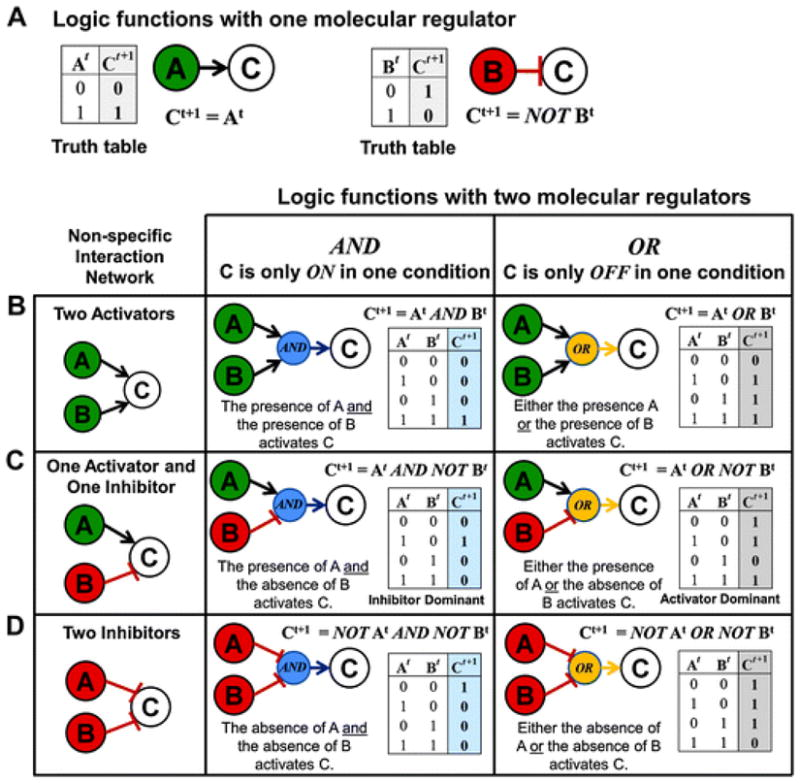
\includegraphics[scale = 0.65]{img/logicnet.jpg}
\end{figure}
In questo esempio notiamo come possiamo differenziare regolazioni positive, come
quella di $A$ su $C$, e quelle negative, come quella di $B$ su $C$, anche a
livello grafico. Notiamo anche come il formalismo sia del tipo:
\[C^{t+1}=\neg B^t\]
indicando con gli apici lo step temporale, avendo quindi specificato che lo
stato risultante in $C$ al tempo $t+1$ dipende da quello di $B$ al tempo
$t$. Ovviamente questi esempi, con le rispettive tabelle diversità, sono
minuscoli, infinitamente più piccoli rispetto a modelli logici
reali. Nell'esempio possiamo comunque vedere le varie casistiche dove $A$ attiva
$C$, facendo regolazione positiva, mentre $B$ lo inibisce, facendo regolazione
negativa, vedendo i vari risultati possibili nelle varie possibili combinazioni
di ``input''.\\
Nel dettaglio, inoltre, lo stato del sistema al tempo $t$ corrisponde ad un
vettore booleano consistente nel valore di ogni variabile booleana al tempo
$t$. Purtroppo a volte non abbiamo informazioni biologiche per assegnare la
funzione booleana al nodo e ovviamente la questione si complica all'aumentare
dei nodi regolatori, positivamente e negativamente, del nodo in
questione. Quindi alla semplicità matematica si associa in questo caso anche un
``lack'' di informazioni biologiche preliminari. \\
Si procede quindi dallo \textit{stato iniziale}, che viene definito per $t=0$, e
si calcola la traiettoria che si ha a partire da quello stato, che viene
composta quindi dall'insieme degli stati a $t=1$, $t=2$, $t=3$ etc$\ldots$ dove
il tempo è una \textbf{variabile discreta}, avendo quindi $\{t,
t+1,t+2,\ldots\}$, e dove si assume aggiornamenti in \textit{modalità sincrona}.
Fatte queste premesse è ovvio che lo stato corrente del sistema è identificato
univocamente dallo stato precedente, che a sua volta identificava univocamente
lo stato corrente come suo successore. Si ha quindi che i \textit{modelli
  logic-based booleani sincroni} sono \textbf{deterministici}, avendo che un
certo input produrrà sempre e solo lo stesso output.\\
Sfruttiamo ora un esempio per caratterizzare meglio \textit{attrattori} e
\textit{bacini di attrazione}.\\
Sia data la seguente rete:
\begin{center}
  \begin{tikzpicture}[shorten >=1pt,node distance=2cm,on grid,auto]
    \node[state] (q_0) {$A$};
    \node[state] (q_1) [below right=of q_0] {$C$};
    \node[state] (q_2) [above right=of q_1] {$B$};
    \path[->]
    
    (q_2) edge  node {} (q_1)
    (q_2) edge  node {} (q_0)
    (q_0) edge [bend left = 25] node {} (q_2);
    \path[-|]
    (q_1) edge  node {} (q_0);
  \end{tikzpicture}
\end{center}
\newpage
\noindent
Alla quale vengono aggiunte le seguenti funzioni booleane:
\begin{itemize}
  \item $f(A)=B\land (\neg C)$
  \item $f(B)=A$
  \item $f(C)=B$
\end{itemize}
Si ha quindi la seguente tabella di verità, che avendo $3$ variabili/nodi avrà
$2^3=8$ possibili combinazioni di stati di nodi, avendo che ogni riga della
tabella di verità rappresenta uno stato della rete:
\begin{table}[H]
  \centering
  \begin{tabular}{c|c|c||c|c|c}
    $A$&$B$&$C$&$f(A)$ & $f(B)$ & $f(C)$\\
    \hline
    0 & 0 & 0 & 0 & 0 & 0\\
    0 & 0 & 1 & 0 & 0 & 0\\
    0 & 1 & 0 & 1 & 0 & 1\\
    0 & 1 & 1 & 0 & 0 & 1\\
    1 & 0 & 0 & 0 & 1 & 0\\
    1 & 0 & 1 & 0 & 1 & 0\\
    1 & 1 & 0 & 1 & 1 & 1\\
    1 & 1 & 1 & 0 & 1 & 1\\
  \end{tabular}
\end{table}
Possiamo quindi distinguere uno \textit{stato iniziale} che comporta un
\textbf{ciclo} o un \textbf{punto fisso}. Infatti, ad esempio, se parto da
$[1,0,0]$ avrò la seguente traiettoria: 
\[[1,0,0]\Rightarrow [0,1,0]\Rightarrow [1,0,1] \Rightarrow [0,1,0]\Rightarrow
  [1,0,1]\Rightarrow\cdots\]
Avendo quindi che si ha un \textbf{ciclo} tra gli stati $[0,1,0]$ e $[1,0,1]$,
che funge da \textit{attrattore}.\\
D'altro canto se si seleziona come \textit{stato iniziale} $[1,1,0]$ avrò la
seguente traiettoria:
\[[1,1,0]\Rightarrow[1,1,1]\Rightarrow[0,1,1]\Rightarrow[0,0,1]
  \Rightarrow[0,0,0]\Rightarrow[0,0,0]\Rightarrow\ldots\]
raggiungendo quindi un \textbf{punto fisso}, un \textit{attrattore}, ovvero lo
stato $[0,0,0]$. Nel dettaglio inoltre, in questo caso semplice e fortuito, il
\textbf{bacino di attrazione} per l'attrattore $[0,0,0]$ e formato da tutte le
traiettorie che partono dagli
stati presenti nella \textit{traiettoria} che parte dallo stato $[1,1,0]$,
ovvero dagli stati dell'insieme (\textbf{capire se attrattore è nel suo stesso
  bacino di attrazione}): 
\[\{[1,1,0],\,\,[1,1,1],\,\,[0,1,1],\,\,[0,0,1],\,\,[0,0,0]\}\]
Data quindi una \textit{rete booleana} e una traiettoria sufficientemente lunga
prima o poi lo stato della rete sarà una ripetizione di una sequenza di stati
già incontrata, questo perché si ha un numero di stati totali \textbf{finito},
in quanto \textbf{discreto}.\\
Visto l'esempio possiamo raffinare quindi quanto già definito:
\begin{itemize}
  \item un \textbf{attrattore} è definito come \textbf{punto fisso
    (\textit{fixed state})} qualora si abbia che un singolo stato appare
  ripetutamente in una \textit{traiettoria}
  \item un \textbf{attrattore} è definito come \textbf{ciclo} se un insieme di
  stati appare più di una volta in una \textit{traiettoria}
\end{itemize}
Avendo quindi che un \textbf{attrattore} rappresenta uno stato dal quale non è
possibile scappare a meno che non si verifichi una \textit{perturbazione}
esterna al sistema stesso mentre un \textbf{bacino di attrazione} è l'insieme di
tutte le traiettorie che terminano in un \textit{attrattore}.
\subsection{Vari Esempi}
Si elencano ora una serie di esempi, tratti da vari paper, per capire meglio la
modellazione tramite \textit{modelli logici booleani}.\\
Un primo esempio è un semplice modello con 12 nodi proposto da Wynn et
al.\footnote{Wynn ML, Consul N, Merajver SD, Schnell S. Logic-based models in
  systems biology: a predictive and parameter-free network analysis
  method. Integr Biol
  (Camb). 2012;4(11):1323-1337. doi:10.1039/c2ib20193c}. Questo esempio, come
visibile in figura \ref{fig:exbool}. Nell'esempio abbiamo infatti, in nella
figura $A$, una prima modellazione del sistema tramite una \textit{rete
  d'interazioni}, con l'aggiunta dei due nodi di \textit{input} e
\textit{output}. Passando alla figura $B$ abbiamo il passaggio alla 
\textit{rete booleana} con la rappresentazione esplicita degli operatori
booleani tramite nodi. Si noti che il nodo \textit{output} non influenza alcun
altro nodo. In figura $C$ abbiamo invece l'elenco delle funzioni logiche che
permettono l'evoluzione della rete. Poi in figura $D$ si hanno vari esempi di
transizione dal tempo $t$ al tempo $t+1$. Si hanno infatti 7 possibili stati
iniziali e la rappresentazione degli stati è fatta in primis tramite una matrice
booleana e quindi tramite l'intero, in base decimale, rappresentato in ogni riga
della stessa. Infine, in figura $E$, abbiamo una rappresentazione esplicita
dall'insieme e degli stati raggiungibili, rappresentati coi ``pallini'', e degli
attrattori. Si noti che quelli nella figura non sono grafi ma una 
rappresentazione degli stati dove i ``pallini'' più esterni rappresentano gli
stati iniziali. Si hanno poi le varie traiettorie rappresentate tramite i
collegamenti tra i vari ``pallini'', avendo quindi una rappresentazione dei
\textbf{bacini di attrazione}, mentre gli \textbf{attrattori} sono specificati
in rosso, avendo che il singolo ``pallino'' rappresenta un \textit{fixed point},
mentre se si hanno più ``pallini'' si ha un \textit{ciclo}, come esplicitato
nello zoom a destra. Si comprende ancora meglio come in questo contesto si abbia
un vero e proprio concetto di \textit{simulazione}, che porta a ottenere le
traiettorie stesse, avendo comunque solo risultati \textit{qualitativi}, per
quanto \textit{dinamici}.  \\
\begin{figure}
  \centering
  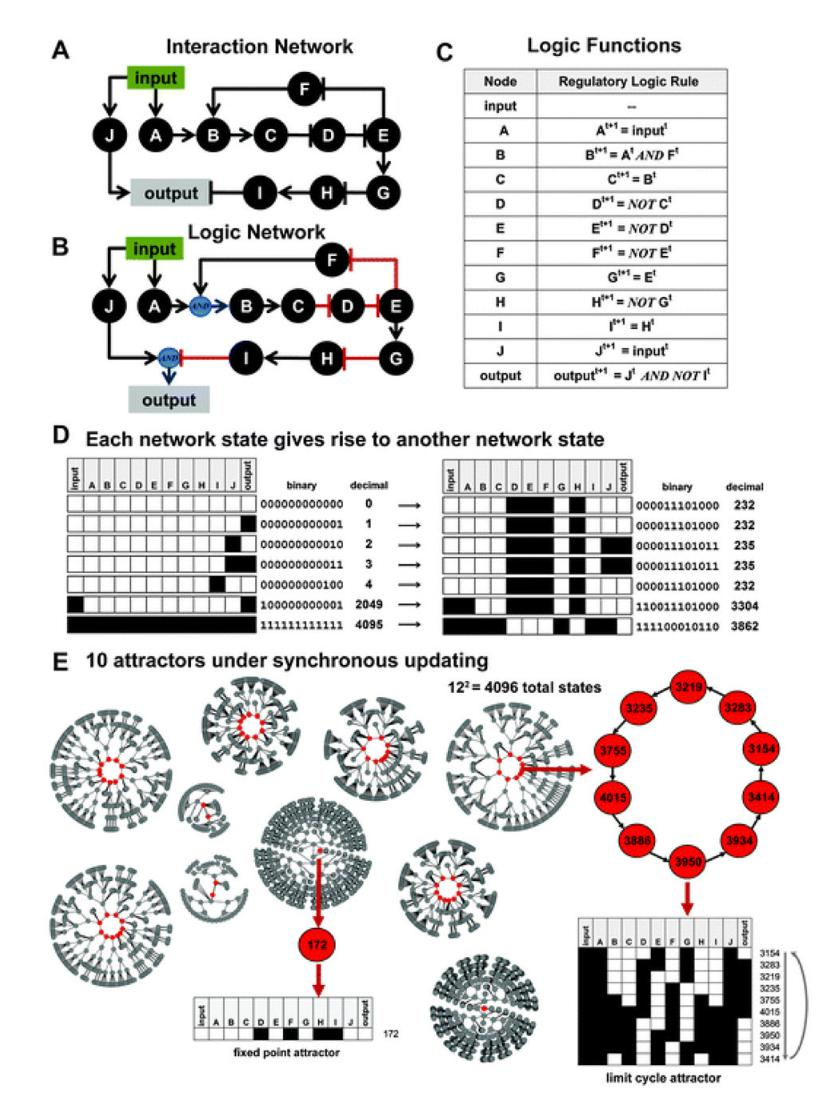
\includegraphics[scale = 0.35]{img/exbool.jpg}
  \caption{Esempio di un \textit{modello logico} tramite \textit{rete
      booleana}.} 
  \label{fig:exbool}
\end{figure}
Interessante è anche notare come, sempre nel lavoro di Wynn et al.\footnote{Wynn
  ML, Consul N, Merajver SD, Schnell S. Logic-based models in 
  systems biology: a predictive and parameter-free network analysis
  method. Integr Biol
  (Camb). 2012;4(11):1323-1337. doi:10.1039/c2ib20193c}, come visibile in figura
\ref{fig:exbool2}, il variare di una singola funzione logica, nell'esempio
\textit{or not} contro \textit{and not}, porti a traiettorie molto diverse con
pochissimi ``punti di contatto''. Non sempre infatti si hanno le basi di
conoscenza per poter modellare con certezza un modello, magari non avendo chiara
specifica a priori di una certa regolazione. Nel modello, nel dettaglio, si
hanno come input, in rosso e verde nella figura:
\begin{itemize}
  \item sovrappopolazione
  \item fattori di crescita
  \item ipossia, ovvero carenza della quantità di ossigeno che raggiunge i
  tessuti 
  \item danni al \textit{DNA}
\end{itemize}
In output, come anticipato, si hanno:
\begin{itemize}
  \item proliferazione
  \item apoptosi
\end{itemize}
Il tutto quindi presenta, assumendo \textit{update sincrono}:
\begin{itemize}
  \item $2^4=16$ stati iniziali
  \item $2^{10}=1024$ possibili stati della rete
  \item $16$ attrattori
\end{itemize}
Si nota come questo tipo di situazione sia anche interessante nello studio del
variare degli output in base al tuning dei vari input, per portare ad un certo
output. \\
\begin{figure}
  \centering
  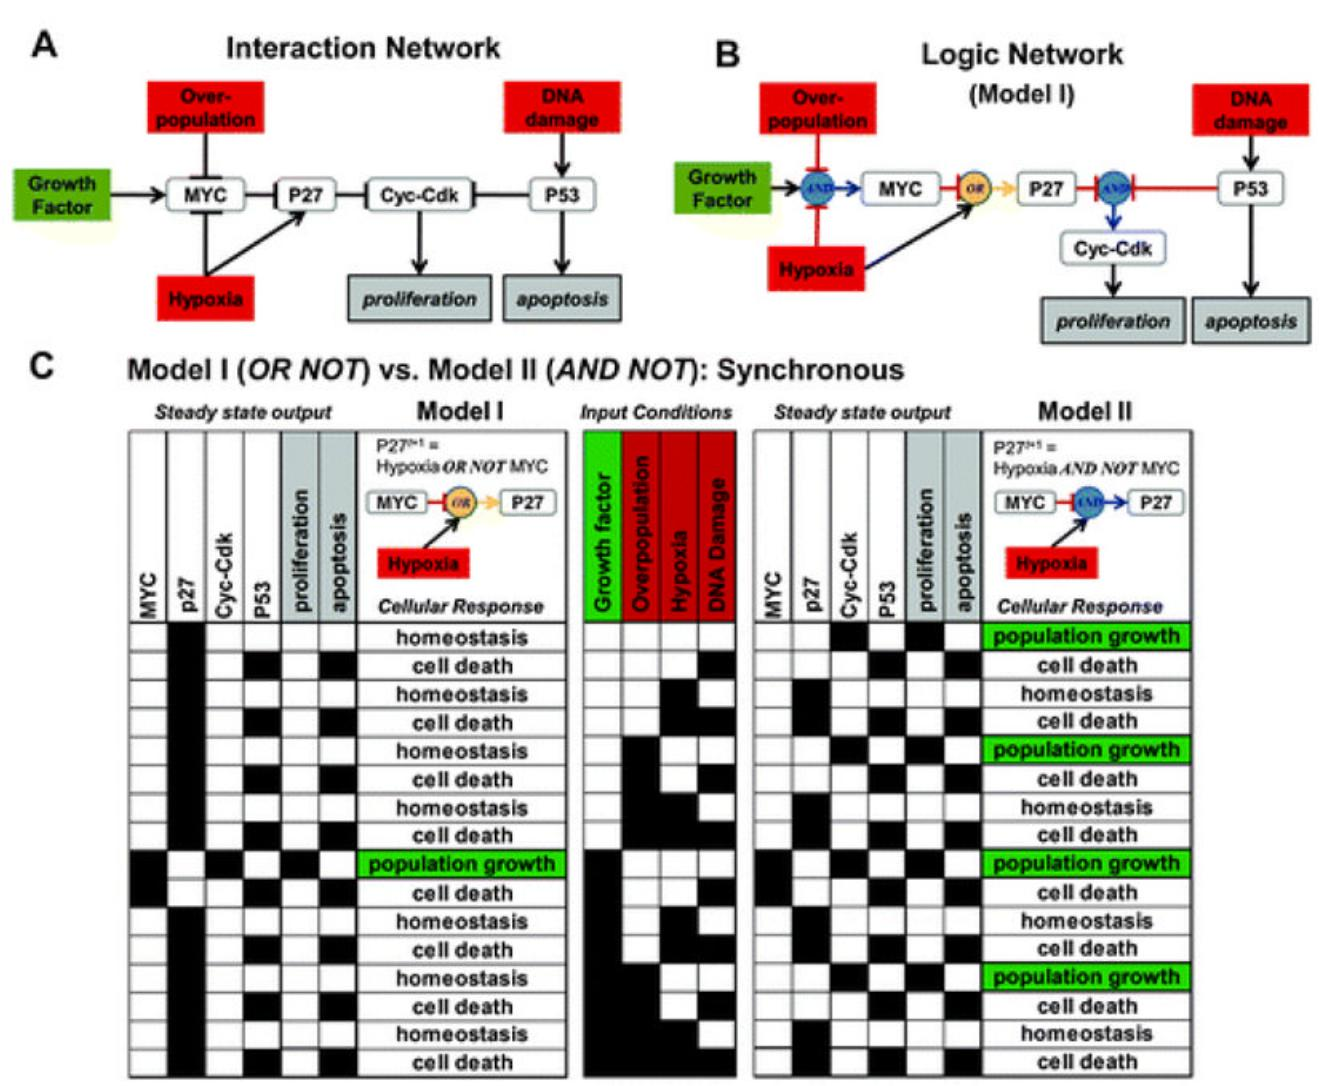
\includegraphics[scale = 0.25]{img/exbool2.jpg}
  \caption{Comparazione di due \textit{modelli logici} tramite \textit{rete
      booleana} per lo studio  della \textit{proliferazione} e
    dell'\textit{apoptosi}, al variare di una singola funzione logica.}  
  \label{fig:exbool2}
\end{figure}
Un altro aspetto fondamentale riguarda l'interpretazione biologica degli
attrattori stessi. Tra le varie interpretazioni si hanno quelle dei
\textit{fenotipi}, ad esempio nello studio della \textit{differenziazione
  cellulare}. Si prende ad esempio il paper di Huang\footnote{Huang,
  Sui. "Reprogramming cell fates: reconciling rarity with robustness." Bioessays
  31.5 (2009): 546-560.}, da dove è tratta la figura \ref{fig:exbool3}. In
questa immagine abbiamo la comparazione tra la \textit{rete booleana} e le sue
traiettorie con quanto ottenibile tramite varie analisi, ai diversi istanti
temporali, con la tecnica dei \textit{microarrays}, che misrano l'espressione
genica, e la produzione della
\textit{mappa GEDI}. Una \textbf{mappa GEDI (\textit{Gene Expression Dynamics
    Inspector})} è una 
rappresentazione visiva di un microarray che riorganizza i geni per creare
pattern caratteristici, che riflettono la somiglianza tra i profili di
espressione. In pratica, in modo parallelo al modello logico, si usano altre
tecniche per caratterizzare lo stato della rete tramite i vari fenotipi. Da qui,
come visibile in figura $E$, posso partire da uno stato cellulare definito a
priori e seguire l'evoluzione del modello anche tramite gli studi in laboratorio
ai vari step temporali, studiando i fenotipi, che vengono quindi ``collegati''
al modello booleano, e quindi le caratteristiche emergenti del modello. Quindi,
iniziamo con una cellula staminale e durante il processo di differenziazione la
cellula cambia e diventa un diverso tipo di cellula. Quindi, lo stato finale è
un'attrazione che è la specializzazione della cellula.  \\
Sempre proseguendo sullo stesso discorso sempre Huang\footnote{Huang,
  Sui. "Reprogramming cell fates: reconciling rarity with robustness." Bioessays
  31.5 (2009): 546-560.} propone anche una rappresentazione grafica degli
\textit{ipotetici stati epigenetici}, quindi legato ai fenotipi, i pallini verdi
in figura \ref{fig:exbool4}. I geni portano la cellula verso una certa
traiettoria, avendo diverse possibilità di ottenere le diverse espressioni
geniche. Questo visivamente si vede avendo che i ``pallini'' verdi si vanno a
posizionare nelle ``conche''. Solo una perturbazione può portare gli stessi
fuori da queste conche. Questo si ricollega anche al discorso delle cellule
staminali, che restano tali per un certo periodo per poi iniziare a
differenziarsi, parlando quindi di \textit{stato quasi-potential} ovvero la
cellula ha la potenzialità di cambiare lo stato anche se è potenzialmente
stabile. Inoltre in questo contesto il fatto che i sistemi logici siano
deterministici può essere limitante nei confronti della stocasticità intrinseca
della natura ma, limitandosi al discorso degli \textit{attrattori}, la si può
accettare come semplificazione valida.\\
Per completezza un altro paper interessante è quello di Graf e
Enver\footnote{Graf T, Enver T. Forcing cells to change
  lineages. Nature. 2009;462(7273):587-594. doi:10.1038/nature08533} dove si ha
un discorso analogo a quello fatto.\\
\begin{figure}
  \centering
  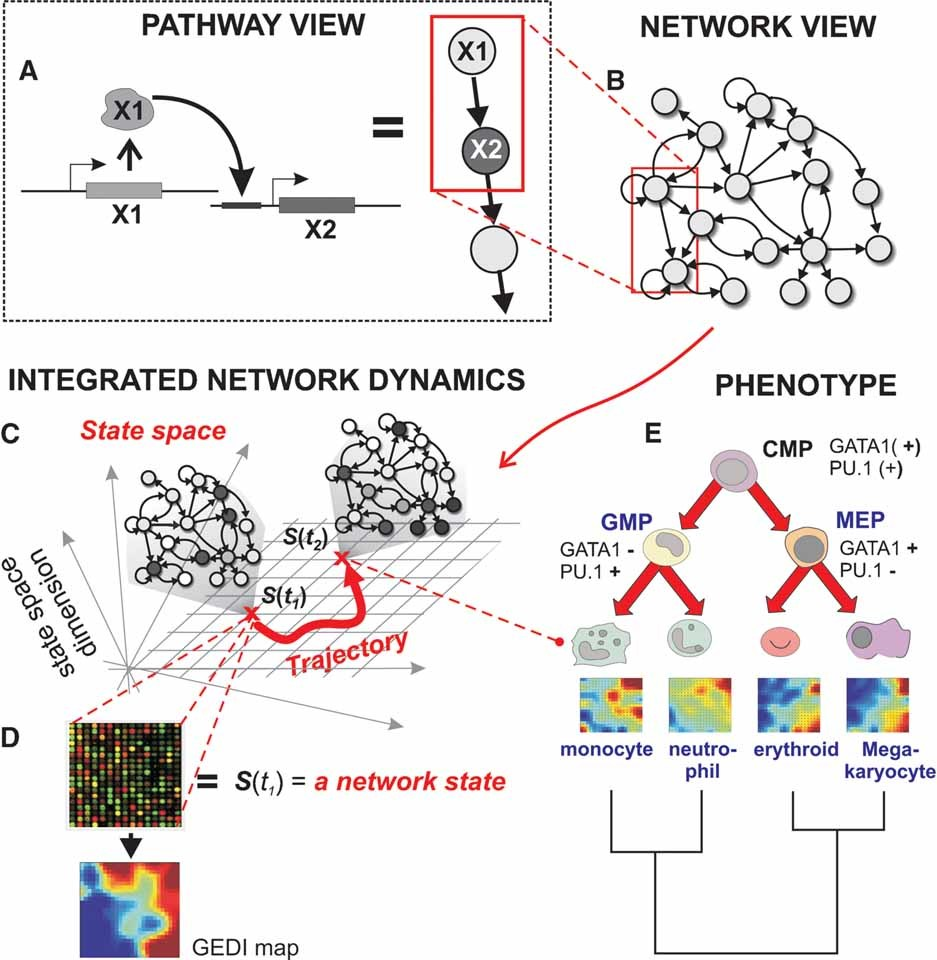
\includegraphics[scale = 0.30]{img/exbool3.jpg}
  \caption{Esempio di comparazione tra una \textit{rete booleana} e altre
    tecniche sperimentali, come le \textit{mappe GEDI}.}  
  \label{fig:exbool3}
\end{figure}
\begin{figure}
  \centering
  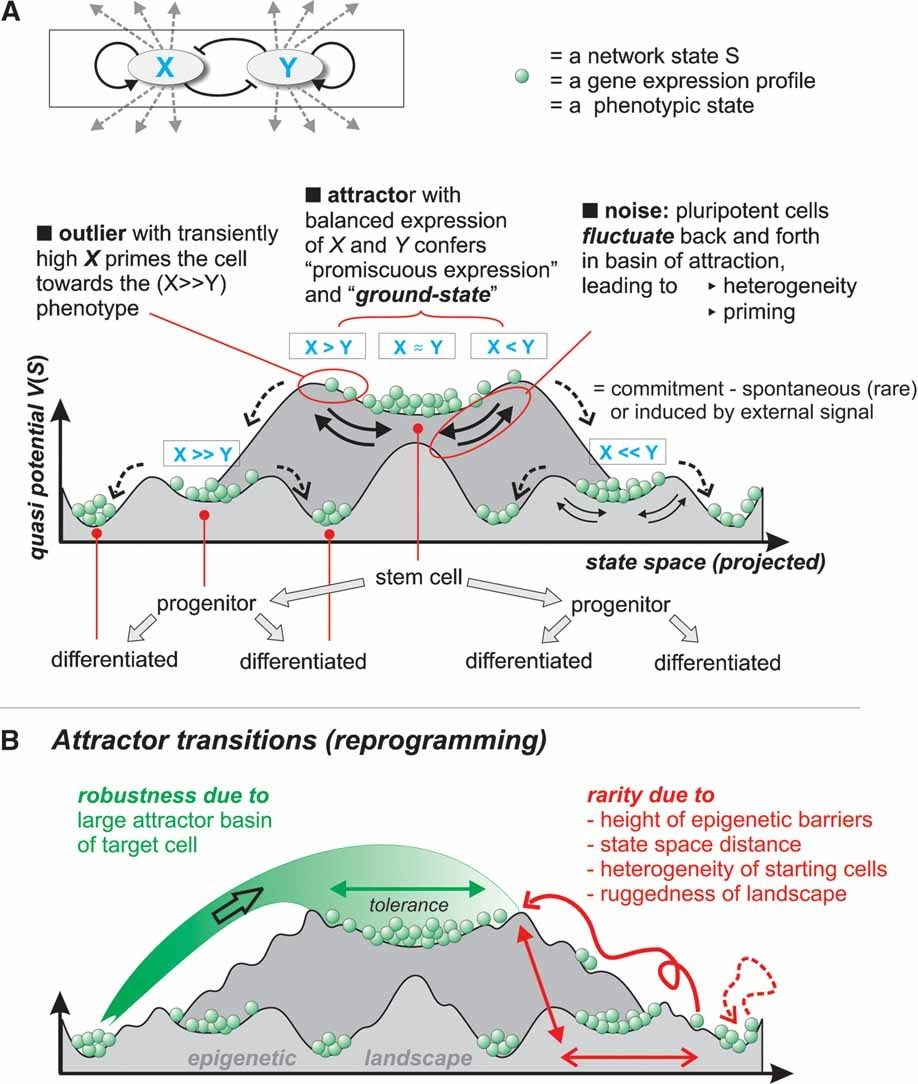
\includegraphics[scale = 0.30]{img/exbool4.jpg}
  \caption{Rappresentazione grafica degli \textit{stati epigenetici}.}  
  \label{fig:exbool4}
\end{figure}
\noindent
Vediamo infine un ultimo esempio, tratto dal lavoro di Udyavar et
al.\footnote{Udyavar AR, Wooten DJ, Hoeksema M, et al. Novel Hybrid Phenotype
  Revealed in Small Cell Lung Cancer by a Transcription Factor Network Model
  That Can Explain Tumor Heterogeneity [published correction appears in Cancer
  Res. 2019 Mar 1;79(5):1014]. Cancer
  Res. 2017;77(5):1063-1074. doi:10.1158/0008-5472.CAN-16-1467} dove si è
studiata la differenza di fenotipi nel caso del \textit{small cell lung
  cancer}. Si avevano infatti principalmente due fenotipi, con caratteristiche e
quindi terapie associate differenti:
\begin{itemize}
  \item \textit{neuroendocrin/epithelial}, \textit{NE}
  \item \textit{non-neuroendocrin/mesenchymal-like}, \textit{ML}
\end{itemize}
che ci si aspettava fossero ben caratterizzati da due attrattori nel modello,
ottenuto tramite 33 fattoti di trascrizione, modello che avrebbe poi permesso di
regolare meglio i dosaggi delle cure etc$\ldots$.\\
I risultati dello studio, visibili
in figura \ref{fig:exbool5}, mostrano non solo come i risultati del modello
siano comparabili a quelli ottenuti sperimentalmente in laboratorio ma conferma
anche l'esistenza di un fenotipo ibrido, un terzo attrattore, conosciuto in
letteratura ma non ben 
caratterizzato, che era quello più aggressivo e difficile da curare. Quindi non
solo tali modelli hanno spazio anche in fase di validazione dei dati
sperimentali ma possono anche essere l'inizio, come spesso in \textit{systems
  biology}, per ulteriori studi, con modelli diversi (magari
\textit{meccanicistici}) ma anche sperimentali in \textit{wet-lab}, fatti al
fine di migliorare la caratterizzazione di quanto scoperto. 
\begin{figure}
  \centering
  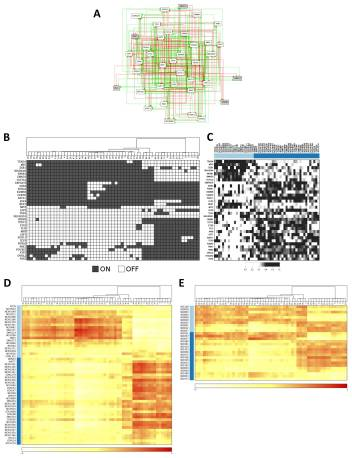
\includegraphics[scale = 0.70]{img/exbool5.jpg}
  \caption{Rete booleana, figura $A$ e vari grafici, ottenuti computazionalmente
    nel caso delle figure $B$ e $C$ e in laboratorio nel caso delle figure
    $D$ ed $E$.}   
  \label{fig:exbool5}
\end{figure}
\\
Un altro esempio interessante, qui solo citato, è quello di Offerman et
al.\footnote{Offermann, Barbara, et al. "Boolean modeling reveals the necessity
  of transcriptional regulation for bistability in PC12 cell differentiation."
  Frontiers in genetics (2016): 44. }. 
\section{Logica Fuzzy}
Sono stati elencati diverse volte i limiti dell'uso della semplice
\textit{logica booleana} per la rappresentazione di sistemi biologici quindi il
prossimo passaggio è quello di sfruttare come logica la \textbf{logica fuzzy},
dove \textit{fuzzy} si può tradurre con il concetto di ``sfumatura''.\\
I sistemi cellulari sono caratterizzati, come già visto, da un alto livello di
\textit{eterogeneità}, avendo interazioni orchestrate tra ioni, metaboliti,
proteine, complessi macromolecolari, vie di trasduzione del segnale, pathway
metabolici, etc$\ldots$ e si sa che lo stato cellulare è normalmente descritto
tramite termini qualitativi dai biologi/biotecnologi, che sono soliti usare
frasi del tipo ``fortemente espresso'', ``moderatamente attivo'' o simili,
evidenziando una forte \textbf{incertezza}, ammessa dalla \textit{logica fuzzy},
della descrizione biologica ed evidenziando anche limiti della misura di dati
sperimentali. \\
Vediamo un breve esempio. Si prenda il seguente sistema\footnote{Nobile M.S. et
  al. Fuzzy modeling and global optimization to predict novel therapeutic
  targets in cancer cells. Bioinformatics, 2019}: 
\begin{figure}[H]
  \centering
  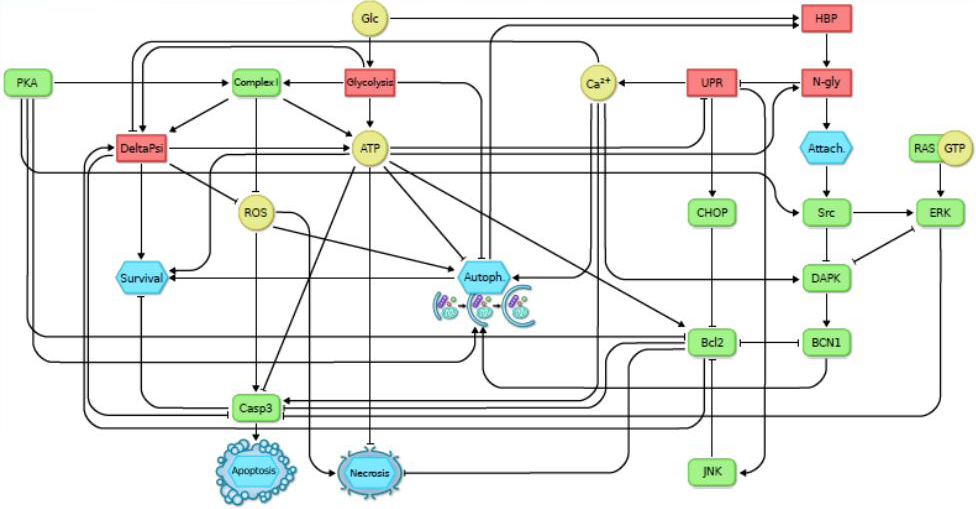
\includegraphics[scale = 1.60]{img/fuz1.jpg}
\end{figure}
Abbiamo un sistema molto eterogeneo che, avendo magari molecole che regolano
processi cellulari o altri regolazioni eterogenee, rappresenta una cellula
cancerogena dalla quale si vuole predire il minimo uso di farmaci per massimare
la morte cellulare tramite apoptosi. Non potrei in questo caso usare modelli
meccanicistici non essendo un sistema \textit{small-scale} e non avendo
praticamente informazioni quantitative.\\
Alla base della \textit{logica fuzzy} si hanno quindi:
\begin{itemize}
  \item un \textbf{grafo diretto} che rappresenta l'insieme dei componenti del
  sistema, corrispondenti a qualsiasi tipo di biomolecole o interi processi
  cellulari, nonché i fenotipi di output, e le loro reciproche regolazioni
  positive o negative  
  \item un insieme di \textbf{variabili linguistiche}, coi corrispondenti
  \textbf{termini linguistici}, e le \textbf{membership function} (introdotte da
  Zadeh nel 1965), per i
  rispettivi \textbf{fuzzy set}, che permettono di dare una descrizione
  qualitativa delle quantità cellulari o dell'attività funzionale. Un altro
  concetto fondamentale è il \textbf{membership degree}, solitamente indicato
  con $\mu$, che caratterizza il valore attutale rispetto ad una
  \textit{membership functions}. Tutti questi caratterizzano i nodi della
  rete.\\ 
  Le \textit{variabili linguistiche} collegano la descrizione qualitativa alla
  rappresentazione quantitativa, qualora si abbia (e in assenza si deriva una
  corrispondenza usando varie tecniche). A differenza dei \textit{modelli
    meccanicistici} non serve la \textit{parametrizzazione del modello}
  \item un insieme di \textbf{regole logiche fuzzy} che specificano lo stato che
  assumerà ciascun componente del sistema in base agli stati dei componenti da
  cui è regolato, permettendo di simulare l'evoluzione del sistema sfruttando
  algoritmi di ragionamento fuzzy e metodi di ``defuzzificazione'', ottenendo
  appunto un \textit{modello dinamico} e \textit{quantitativo}, come in natura
\end{itemize}
\newpage
\noindent
Vediamo ora qualche grafico chiarificatore, dove si comparano \textit{fuzzy set}
con \textit{crisp set}, che è un altro nome per descrivere il caso booleano ma
usando variabili linguistiche. Vediamo infatti un semplice
grafico\footnote{Toksöz Hozatlıoğlu, Derya, and Işık Yılmaz. "A Fuzzy
  Classification Process for Swelling Soils." Transportation Infrastructure
  Geotechnology (2022): 1-14.}:
\begin{figure}[H]
  \centering
  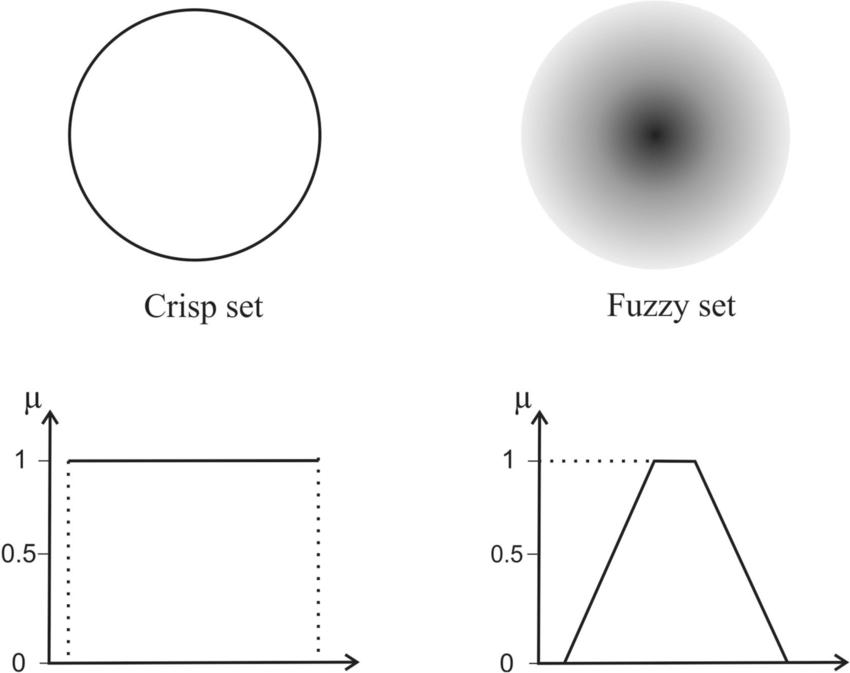
\includegraphics[scale = 1.2]{img/cri.png}
\end{figure}
che ci permette di distinguere chiaramente i due casi:
\begin{itemize}
  \item con il \textit{crisp set} si potrebbe dire che ``o è bianco o è nero'',
  oppure ``o si è dentro o si è fuori'', proprio come nel caso booleano 0/1,
  avendo infatti che posso avere solo o $\mu=0$ o $\mu=1$
  \item con il \textit{fuzzy set} o tutta la casistica intermedia, vendo, per
  assonanza con l'esempio appena fatto, la ``scala di grigi'', con $\mu\in
  [0,1]$, avendo che assume valori reali, pur ricordando che non si tratti
  assolutamente di una probabilità. Inoltre la somma dei vari $\mu$ per un
  certo elemento sull'asse $x$ rispetto a tutti i \textit{fuzzy set} può essere
  maggiore di 1
\end{itemize}
Usando i \textit{termini linguistici} potremmo anche avere il seguente esempio:
\begin{figure}[H]
  \centering
  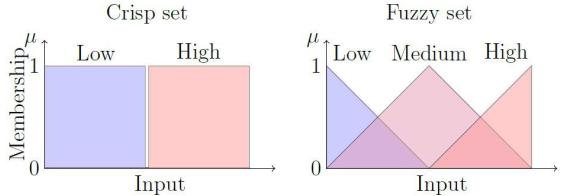
\includegraphics[scale = 0.5]{img/cri.jpg}
\end{figure}
Dove possiamo vedere come nel \textit{crisp set} ci sia solo \textit{low/high}
per un valore che vive sull'asse delle $x$ mentre per il \textit{fuzzy set} ci
siano vari livelli, al variare di $\mu$ per i tre \textit{fuzzy set}. Sono
proprio i \textit{fuzzy set} a permettere di modellare l'\textit{incertezza} in
quanto sfruttano i vantaggi dei \textit{termini linguistici}:
\begin{itemize}
  \item descrivono la vaghezza dei concetti
  \item collegano rappresentazioni qualitative e quantitative
  \item sono vicini al linguaggio naturale
\end{itemize}
Riprendendo quindi l'esempio:
\begin{itemize}
  \item \textit{Low, Medium} e \textit{High} sono i \textit{termini
    linguistici}, qualitativi. Potrei avere dei \textit{modificatori
    linguisitici} per aggiungere anche, ad esempio, \textit{very} a \textit{Low}
  per ottenere \textit{very Low} ma nel caso semplice, che si tratta nel corso,
  questo sarebbe un altro 
  \textit{fuzzy set} e non qualcosa di ottenibile tramite modificatori 
  \item \textit{Input}, che caratterizza l'asse $x$ è il termine quantitativo
  (potrei avere una temperatura, l'età etc$\ldots$) ed è una anch'essa una
  \textit{variabile 
    linguistica} che rappresenta il mio \textbf{universe of discourse}
  \item per ogni \textit{termine linguistico} si ha il relativo \textit{fuzzy
    set} che possono avere forme diverse ma devono coprire tutto l'asse delle
  $x$ tramite la rispettiva \textit{membership function}
\end{itemize}
Bisogna però capire come siano le regole con la \textit{logica fuzzy}. Si assuma
di avere un insieme di nodi $V=\{v_1,v_2,\ldots,v_n\}$ ognuno specificato da
una variabile linguistica. Lo stato di ognuno di questi nodi è
caratteri da un \textit{termine linguistico}. Dato quindi un nodo $v_i$,
regolato da un certo insieme di nodi $V'=\{v_k, v_j, \ldots, v_l\}$ la
\textit{regola fuzzy} per $v_i$ è definita da un insieme di cosiddetti
\textbf{if-then statement}, avendo che lo stato dei nodi in $V'$ funge da
\textbf{antecedente} alla regola, essendo nell'\textit{if}, e lo stato del nodo
$v_i$ è il \textbf{conseguente} della regola, essendo nel \textit{then}.\\
Si ha un breve esempio, con due input (\textit{service} e \textit{food}) e un
output, \textit{tip}, che descrive il processo di scelta di dare o meno una
manca al ristorante, in figura \ref{fig:fuze}.
\begin{figure}
  \centering
  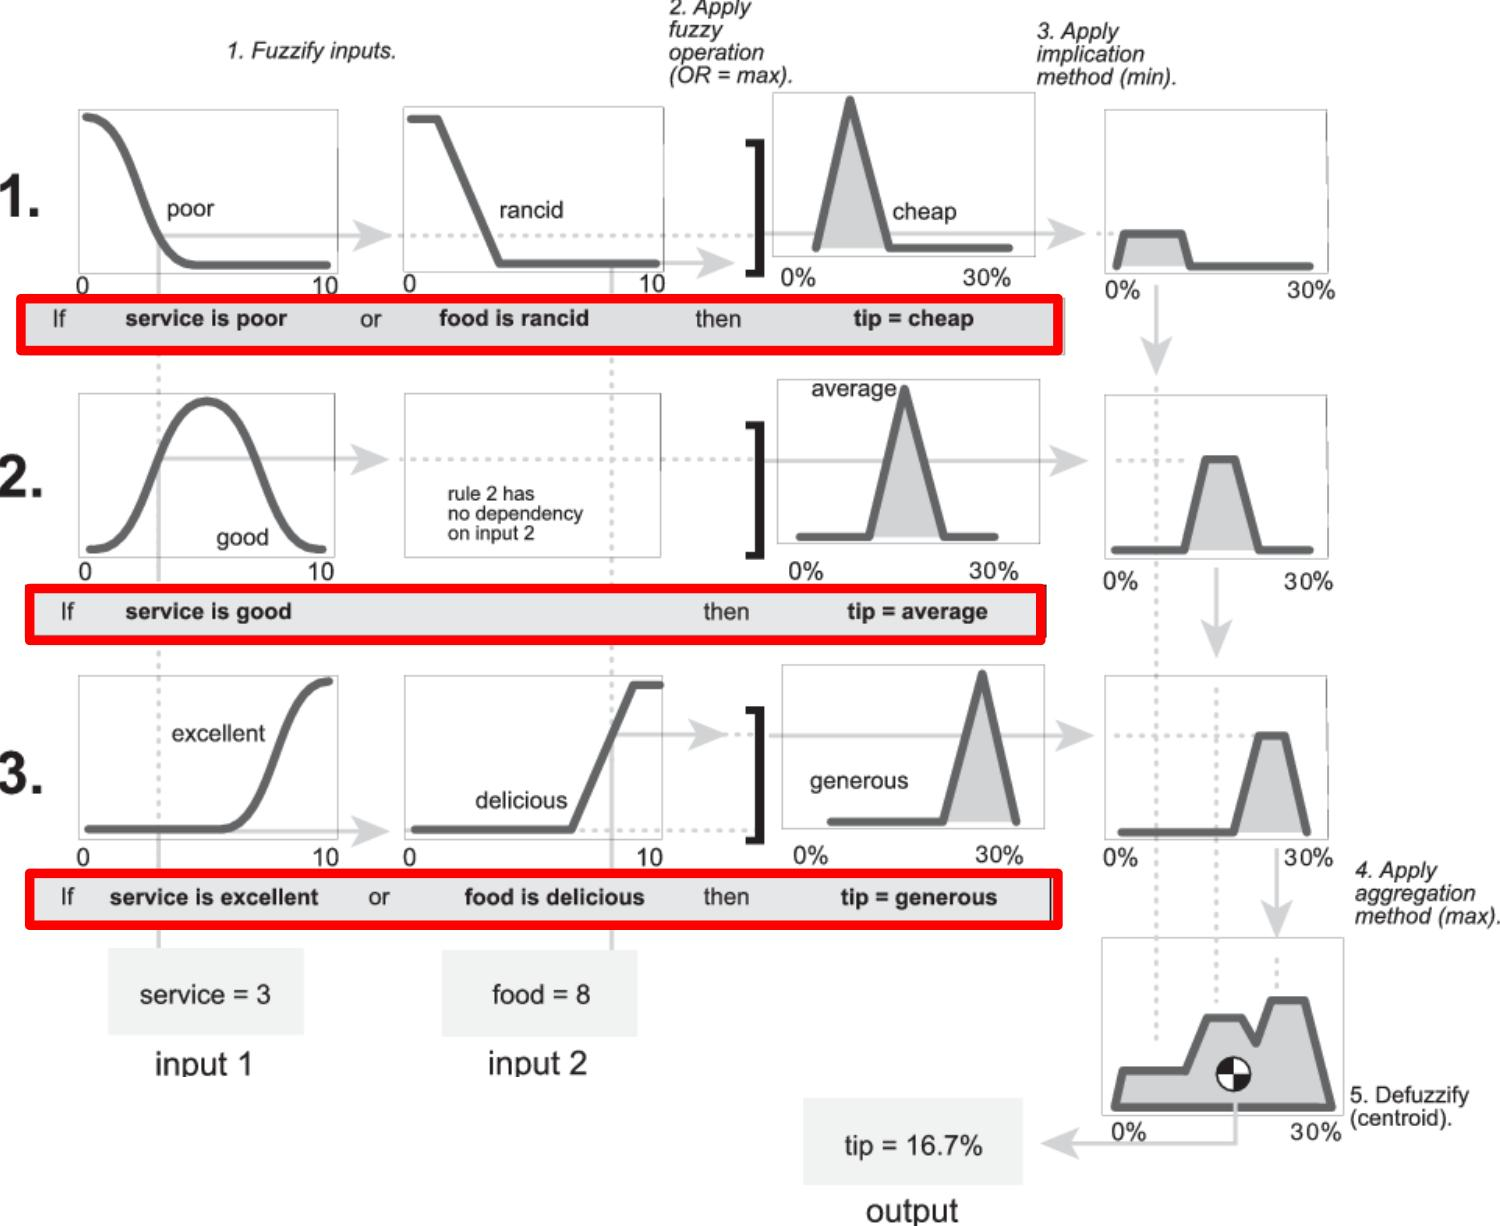
\includegraphics[scale = 1]{img/fuze.jpg}
  \caption{Esempio dove, come regola di \textit{or}, si usa il $\max$
    tra i due 
    valori mentre le tre regole logiche sono bordate in rosso e sono scelte a
    propri 
    o in modo \textit{knowledge-driven}, se possibile quindi partendo dalla
    letteratura, o \textit{data-driven}, soluzione tendenzialmente meno efficace
    e non preferibile che parte dai dati. Le regole vengono valutate
    simultaneamente per ottenere lo stato al tempo $t+1$ partendo dal tempo
    $t$. I 
    $\mu$ degli input serviranno a calcolare il $\mu$ dell'output.}
  \label{fig:fuze}
\end{figure}
\newpage
\section{Seminario Logica Fuzzy}
\textit{Viene qui messo un riassunto del seminario tenuto dal dottor Simone
  Spolaor sulla modellistica tramite logica fuzzy}.\\
La \textbf{logica fuzzy} ha visto la sua nascita nel 1965 per mano di Lotfi
Zadeh del quale si possono citare alcune frasi importanti:
\begin{center}
  ``\textit{I had greatly underestimated the difficulty of designing machines
    that can approximate to the remarkable human ability to reason and
    make decisions in an environment of uncertainty and imprecision} ``
\end{center}
\begin{center}
  ``\textit{We need a radically different kind of mathematics, the mathematics
    of fuzzy or cloudy quantities which are not describable in terms of
    probability distributions}``
\end{center}
Negli anni settanta e ottanta, soprattutto in Giappone, si è avuto un ``boom''
nell'uso della 
\textit{logica fuzzy}, che si poneva a metà tra i modelli logici e quelli
meccanicistici, la quale è stata usata per moltissime soluzioni, tra cui:
\begin{itemize}
  \item robot autonomi
  \item vari usi nella metropolitana in Giappone (il sistema frenante è tutt'ora
  gestito tramite \textit{logica fuzzy})
  \item macchinari per le pulizie
  \item $\ldots$
\end{itemize}
Inoltre tra gli anni ottanta e novanta si sono aggiunti moltissimi lavori
teorici che usavano i \textit{fuzzy set} nel paradigma scientifico, infatti la
\textit{logica fuzzy} può essere applicata per aumentare l'interpretabilità dei
modelli e/o fornire approssimazioni convenienti di comportamenti dinamici
noti. Si hanno infatti modelli che sono semplici da spiegare, ad esempio, a
biologi/biotecnologi (molto di più di un insieme di \textit{EDO}), avendo quindi
che il loro uso ha preso piede sia nell'ambito della modellazione biologica, di
natura estremamente eterogenea etc$\ldots$, che in quello
degli studi clinici. Un altro vantaggio è che tale logica è parsimoniosa dal
punto di vista dei parametri e quindi si ha meno costo computazionale, avendo di
conseguenza meno costo monetario.\\ 
Come si è già accennato le regole della \textit{logica fuzzy} sono basate sui
cosiddetti \textit{if-then statement} dove:
\begin{itemize}
  \item la parte dell'\textit{if} è detta \textit{antecedente}
  \item la parte del \textit{then} è detta \textit{conseguente}
\end{itemize}
Si hanno quindi statement condizionali in cui gli antecedenti sono soddisfatti
in una certa misura, avendo poi la necessità di aggregare l'output di diverse
regole studiate in modo simultaneo. In oltre l'antecedente può essere formato da
più variabili che vengono elaborate insieme mediante operatori logici. Il
significato di tali operatori logici non è standard ma nella maggior parte delle
casistiche si ha:
\begin{itemize}
  \item $\land \implies \min()$
  \item $\lor  \implies \max()$
  \item $\neg \implies 1-\mu$
\end{itemize}
Quindi ad esempio potremmo avere le seguenti regole:
\begin{itemize}
  \item \textit{IF A is High AND B is Low THEN C is High}
  \item \textit{IF A is High OR B is Low THEN C is High}
  \item \textit{IF A is NOT High THEN B is High}
\end{itemize}
Per lo studio dell'insieme delle varie formule si ha quindi bisogno di un
\textbf{sistema di inferenza fuzzy}, ovvero un insieme di \textit{variabili
  linguistiche} e \textit{regole fuzzy}, che quindi consiste nel processo di
mapping di un dato input in un output mediante \textit{logica fuzzy}, dove sia
l'input che l'output sono \textit{crisp}, nel senso che sono valori precisi
della variabile linguistica che vive sull'asse delle $x$. Questo processo può
essere riassunto come in figura \ref{fig:fproc}.
\begin{figure}
  \centering
  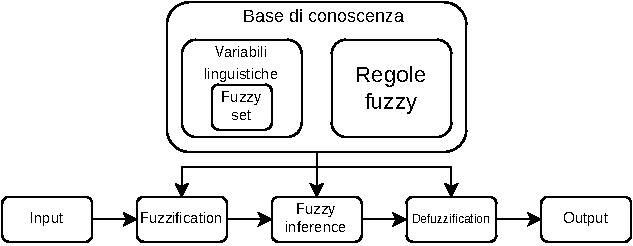
\includegraphics[scale = 1]{img/fproc.pdf}
  \caption{Schema generale del funzionamento di un sistema di inferenza fuzzy.}
  \label{fig:fproc}
\end{figure}
Si hanno due principali metodi di inferenza:
\begin{itemize}
  \item il \textbf{metodo Mandani}
  \item il \textbf{metodo Takagi-Sugeno-Kang (\textit{TSK})}, spesso indicato
  anche solo con \textbf{metodo Sugeno}
\end{itemize}
\subsection{Metodo Mandani}
Il \textbf{metodo Mandani} è stato il primo metodo proposto, nel 1974, per
l'\textit{inferenza fuzzy} e consta di cinque step:
\begin{enumerate}
  \item \textit{fuzzificazione dell'input}
  \item \textit{applicazione degli operatori fuzzy}
  \item \textit{implicazione}
  \item \textit{aggregazione degli output}
  \item \textit{defuzzificazione}, step opzionale
\end{enumerate}
Possiamo quindi riassumere tutto con un esempio grafico\footnote{Simone
  Spolaor}: 
\begin{figure}[H]
  \centering
  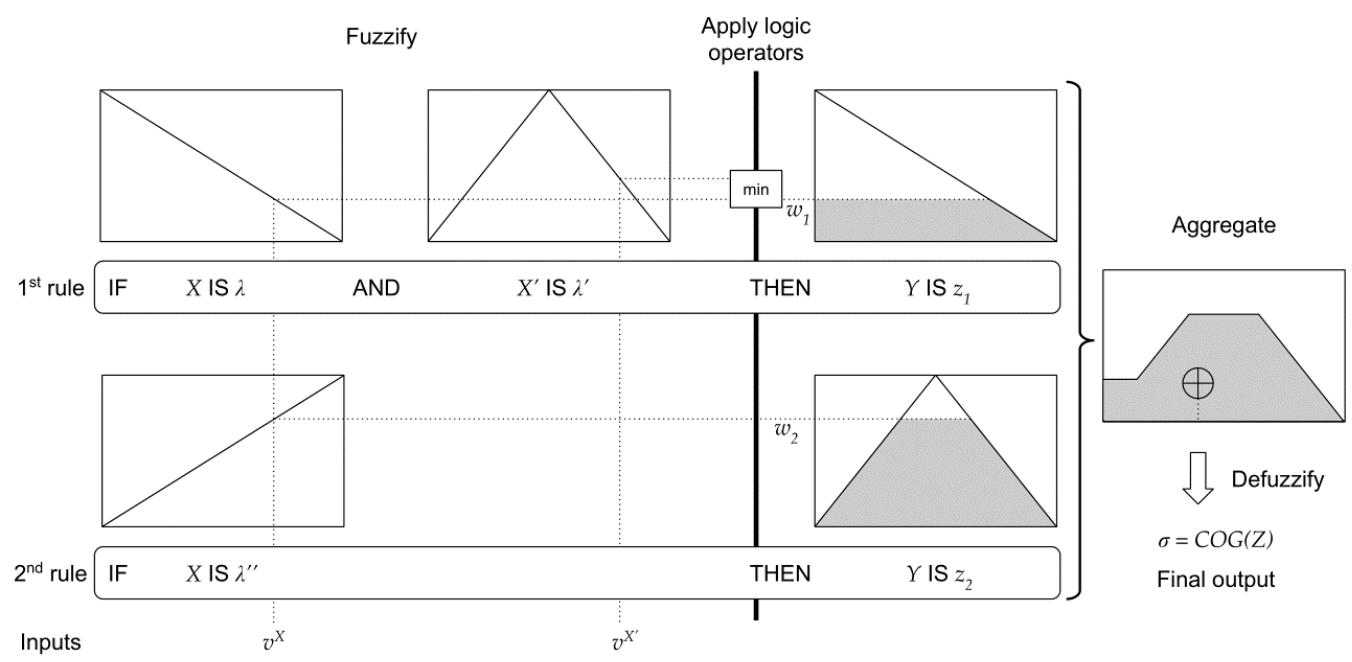
\includegraphics[scale = 0.27]{img/mandani.jpg}
\end{figure}
Nell'esempio si vede l'applicazione di due regole, dati due input $v^X$ e
$v^{X'}$. Il conseguente è un \textit{fuzzy set}. Si nota come con la fase di
aggregazione si produce un poligono di 
forma non banale che subisce la fase di defuzzificazione come applicazione del
calcolo del \textit{COG}, ovvero \textit{center of gravity}, per ottenere poi,
tramite proiezione del risultato sull'asse delle $x$, l'ouptut dell'intero
processo. Il calcolo del \textit{COG} è computazionalmente molto oneroso,
soprattutto con aree non banali. S
nota quindi come il metodo dipenda fortemente ai metodi di
aggregazione/defuzzificazione e che l'applicazione di molte regole possa dare
risultati anche inaffidabili, a causa della creazione di un poligono troppo
complesso. Quindi, per quanto il metodo sia di facile interpretazione,
solitamente non viene utilizzato.
\newpage
\subsection{Metodo TSK}
Il \textbf{metodo TSK (\textit{Takagi-Sugeno-Kang})} è invece uno dei metodi più
usati ed è formato da quattro step:
\begin{enumerate}
  \item \textit{fuzzificazione dell'input}
  \item \textit{applicazione degli operatori fuzzy}
  \item \textit{implicazione}
  \item \textit{aggregazione degli output}
\end{enumerate}
Possiamo quindi riassumere tutto con un esempio grafico\footnote{Simone
  Spolaor}: 
\begin{figure}[H]
  \centering
  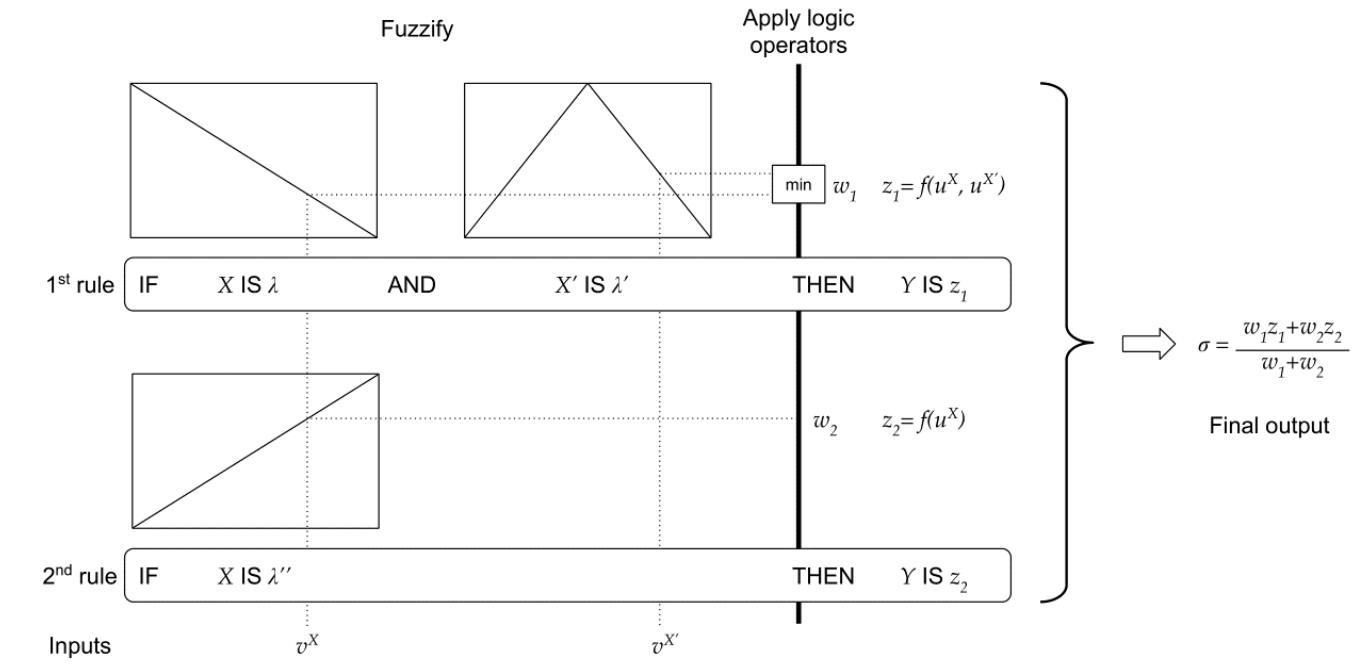
\includegraphics[scale = 0.27]{img/tsk.jpg}
\end{figure}
Si nota come, a differenza del \textit{metodo Mandani}, il conseguente sia in
questo caso una funzione $f$, che può essere lineare, gaussiana etc$\ldots$
essendo quindi più o meno complessa a seconda del caso e della necessità. Non si
ha inoltre in ogni caso la necessità della defuzzificazione avendo che l'ouptut
si ottiene tramite una \textit{media pesata}, riducendo quindi molto il costo
computazionale e garantendo un output più affidabile. Purtroppo funzioni di
ordine superiore portano a una minore interpretabilità.
\newpage
\subsection{Modelli Fuzzy Dinamici}
Dopo aver introdotto i metodi di inferenza bisogna passare ai modelli. Nel 2010
Gegov propose il concetto di \textbf{modello dinamico fuzzy} come un modello
basato su una \textbf{rete di inferenza fuzzy}, avendo quindi una
rappresentazione formale tramite grafo dove i nodi rappresentano le
\textit{variabili linguistiche} mentre gli archi le \textit{regole fuzzy}. Si è
ottenuto quindi un formalismo che può essere adottato per modellare e simulare
l'evoluzione temporale di sistemi eterogenei, a livello di dettaglio
macroscopico.
\subsection{Modello della Morte Cellulare Programmata}
\textit{Si illustra ora un esempio d'uso dei modelli basati su logica fuzzy
  tramite una ricerca svolta dal dottor Spolaor, dalla professoressa Besozzi et
  al.}\\
Lo scopo principale di questa ricerca era rispondere alla domanda:
\begin{center}
  \textit{Come possiamo indurre l'apoptosi nelle cellule tumorali, con una
    quantità minima di farmaci?} 
\end{center}
La morte cellulare programmata è infatti un processo biochimico complesso,
infatti:
\begin{itemize}
  \item include diversi distretti cellulari tra cui \textit{ER (endoplasmic
    reticulum), mitocondri, 
    superficie cellulare, etc}$\ldots$
  \item include diversi attori biochimici, che vanno dalle piccole molecole agli
  organelli interi
  \item tutte le componenti sono fortemente connesse
\end{itemize}
Inoltre i dati disponibili, \textit{sull'espressione genica, sull'imaging a
  fluorescenza etc$\ldots$}, sono di natura qualitativa ed eterogenea e
gli squilibri in questo processo sono coinvolti in diverse malattie complesse,
incluso il cancro.\\
Questo è stato il primo tentativo di modellare tale processo tramite
\textit{modelli dinamici fuzzy} in quanto in letteratura erano presenti solo
\textit{modelli basati su reti booleane}.
\newpage
\noindent
Si è quindi arrivati al modello già
visto precedentemente\footnote{Nobile M.S. et al. Fuzzy modeling and global
  optimization to predict novel therapeutic 
  targets in cancer cells. Bioinformatics, 2019}: 
\begin{figure}[H]
  \centering
  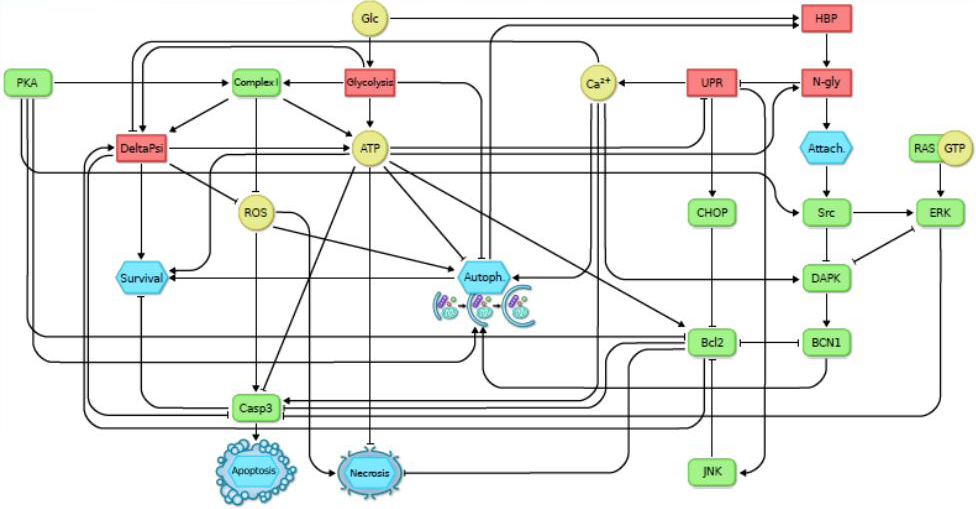
\includegraphics[scale = 1.60]{img/fuz1.jpg}
\end{figure}
Dove si contavano 25 \textit{variabili linguistiche} e ben 252 \textit{formule
  fuzzy} elaborate a mano in modalità \textit{knowledge-driven}. Il modello si
è dimostrato buono dopo una validazione tramite studi \textit{in-vitro} e quindi
è potuto procedere a studiare le simulazioni del modello in presenza di
\textit{perturbazioni}, con l'idea di cercare la combinazione minima di
variabili perturbate in grado di massimizzare la morte apoptotica e ridurre al
minimo la sopravvivenza, avendo che la \textit{perturbazione} viene scelta tra i
termini linguistici disponibili di ciascuna variabile. Si noti che la
\textit{perturbazione} di una variabile non avviene mediante il \textit{metodo
  TSK}.\\
Per procedere con l'analisi è quindi usato un \textbf{algoritmo di
  ottimizzazione globale}, che studia il cosiddetto \textit{spazio delle
  soluzioni}. Senza entrare nei dettagli un problema di
ottimizzazione consiste nel trovare una soluzione ottimale a un dato
problema. Si inoltre ha la \textbf{fitness function} che misura la qualità delle
soluzioni possibili, funzione della quale bisogna trovare l'ottimo per risolvere
un problema di ottimizzazione. \\
Nel dettaglio della ricerca si aveva uno \textit{spazio delle soluzioni} che
conteneva $3^6 \cdot 4^9 = 191102976$ possibili soluzioni. Per gestire uno
spazio delle soluzioni così ampio si è scelto di usare uno degli algoritmi più
famosi di ottimizzazione globale: l'algoritmo detto \textbf{Simulated
  Annealing}, che ottimizzava la seguente funzione di fitness:
{\small{\[F(\pi)=\frac{\left[s_{apoptosis}^\pi(t_b+\delta)-
          s_{apoptosis}^\pi(t_b)\right] -\left[s_{survival}^\pi(t_b+\delta)-
          s_{survival}^\pi(t_b)\right]}{\delta\cdot|\pi|}\] }}
Dove:
\begin{itemize}
  \item $\pi$ è la perturbazione, avendo $F(\pi)$ come funzione di fitness
  \item $|\pi|$ è il numero di variabili perturbate da $\pi$
  \item $\delta$ è il tempo dopo il quale viene valutato l'effetto della
  perturbazione 
  \item $\left[s_{apoptosis}^\pi(t_b+\delta)-s_{apoptosis}^\pi(t_b)\right]$ è
  il cambiamento per quanto riguarda l'apoptosi con l'azione della
  perturbazione
  \item $\left[s_{survival}^\pi(t_b+\delta)-s_{survival}^\pi(t_b)\right]$ è
  il cambiamento per quanto riguarda la sopravvivenza con l'azione della
  perturbazione
\end{itemize}
\textit{Non si entra nei dettagli della formula, in caso consultare il paper di
  riferimento\footnote{Nobile M.S. et al. Fuzzy modeling and global optimization
    to predict novel therapeutic 
    targets in cancer cells. Bioinformatics, 2019}}.\\
Ovviamente il range delle possibili soluzioni è stato anche testato in
\textit{wet-lab} ma si cercavano col modello bersagli per nuovi trattamenti
chemioterapici. Tali bersagli erano, nel dettaglio:
\begin{itemize}
  \item \textit{UPR activation}
  \item \textit{Complex I inhibition}
  \item \textit{UPR activation and autophagy inhibition}
  \item \textit{HBP and N-glycosylation inhibition}
  \item \textit{N-glycosylation and autophagy inhibition}
\end{itemize}
I vari studi sono stati molto complessi e difficili da ottenere ma hanno portato
a scoperte interessanti.\\
La domanda iniziale però è stata raffinata:
\begin{center}
  \textit{Possiamo ottenere soluzioni di dimensioni minime, massimizzando
    l'apoptosi e riducendo al minimo la necrosi?} 
\end{center}
Si è quindi passati ad un \textbf{problema di ottimizzazione
  multi-obiettivo}. Tale classe di problemi ha solitamente più di una soluzione
ottima, che possono essere rappresentate da un cosiddetto \textit{Pareto front},
che è un insieme che rappresenta tutte soluzioni egualmente ottimali,
rappresentando 
anche i vari ``tradeoff'', da bilanciare con le varie soluzioni ottime, tra i
vari obiettivi. \\
Si è quindi ripetuta l'analisi perturbativa sul modello di morte cellulare
programmata, questa volta ottimizzando tre diversi obiettivi\footnote{Spolaor
  S. et al. Screening for Combination Cancer Therapies With Dynamic Fuzzy
  Modeling and Multi-Objective Optimization. Frontiers in Genetics, 2021}: 
\begin{enumerate}
  \item massimizzare l'apoptosi
  \item minimizzare la necrosi
  \item minimizzare il numero di variabili perturbate
\end{enumerate}
\textit{Questo discorso non viene approfondito}.\\
Interessante notare come l'uso di \textit{modelli dinamici fuzzy} sia cruciale
in altri progetti in corso (fatti in collaborazione con la Fondazione Tettamanti
e l'Università dell'Insubria), tra cui:
\begin{itemize}
  \item modellazione dell'insorgenza della \textit{Precursor B cell Acute
    Lymphoblastic Leukemia (BCP-ALL)} in pazienti pediatrici
  \item previsione della risposta terapeutica nei pazienti pediatrici affetti da
  \textit{T cell Acute Lymphoblastic Leukemia (T-ALL)}  
  \item modellazione della rete mitocondriale disfunzionale nella
  \textit{malattia di Parkinson}  
\end{itemize}
\subsection{Simpful}
Al fine di poter effettuare simulazioni tramite \textit{modelli dinamici fuzzy}
il dottor Spolaor ha sviluppato una libreria in \textit{python}, chiamata
\textbf{simpful}\footnote{Spolaor S. et al. Simpful: A User-Friendly Python
  Library for Fuzzy Logic. International Journal of Computational Intelligence
  Systems, 2020} per usare la \textit{logica fuzzy} e di conseguenza modellare
\textit{modelli dinamici fuzzy}. Un esempio è visibile al listing
\ref{lst:fuzzyrepr}.\\ 
Sono attualmente supportate le seguenti funzionalità:
\begin{itemize}
  \item \textit{fuzzy set} con funzioni poligonali e/o personalizzate
  \item definizione di regole fuzzy come stringhe di testo
  \item regole logiche arbitrariamente complesse costruite con operatori logici
  classici, $\land,\lor,\neg$
  \item \textit{metodo TSK}per l'inferenza a qualsiasi ordine
  \item varie utility per i plot
\end{itemize}
Il core della libreria consiste nell'eseguire un'analisi ricorsiva delle regole
per costruire rappresentazioni eseguibili degli antecedenti, sotto forma di
\textit{alberi di derivazione}.
\begin{listing}
  \scriptsize
  \inputminted{python}{code/fuzzy_repr.py}
  \caption{Esempio del repressilator modellato tramite logica fuzzy. Altri
    esempi sono disponibili presso
    \url{https://github.com/aresio/simpful/tree/master/examples}} 
  \label{lst:fuzzyrepr}
\end{listing}
\section{Note Conclusive}
Si mettono ora alcune ultime note riguardo questa categoria di modelli.\\
Come visto nel capitolo ci si è focalizzati soprattutto su \textit{modelli
  booleani} e su \textit{modelli basati su logica fuzzy}. In realtà si hanno
molte altre varianti, come visibile in figura \ref{fig:logmod}\footnote{Le
  Novère N. Quantitative and logic modelling of molecular and gene networks. Nat
  Rev Genet. 2015;16(3):146-158. doi:10.1038/nrg3885}, dove le varie soluzioni
vengono catalogate in base a come sono caratterizzati le variabili e a come
viene rappresentato il tempo. Nella figura si inizia a mostrare un confronto tra
\textit{modelli logici} e \textit{modelli meccanicistici}, confronto che verrà
approfondito anche più avanti nel corso.
\begin{figure}
  \centering
  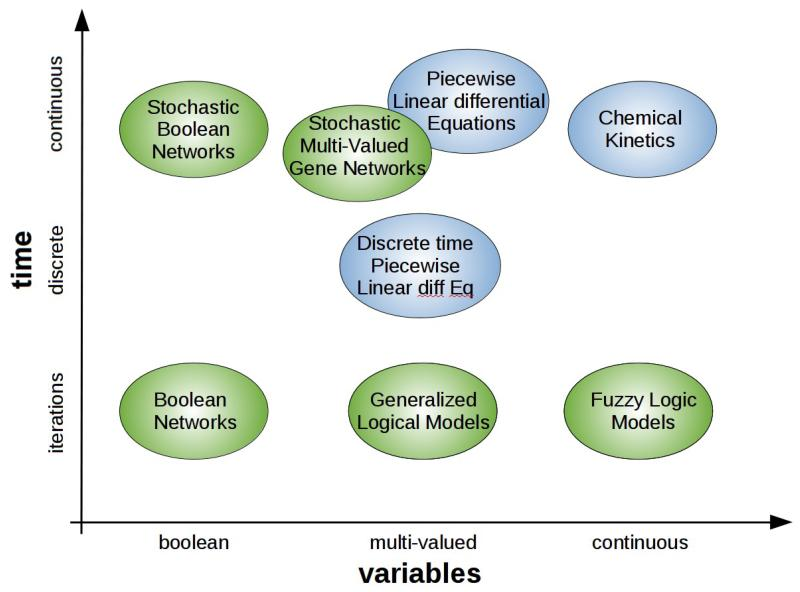
\includegraphics[scale = 0.8]{img/logmod.jpg}
  \caption{Overview delle varie tipologie di modelli logici, in verde, e di
    alcuni tipi di modelli meccanicistici, in blu.}
  \label{fig:logmod}
\end{figure}
\section{Software}
Per lo studio di modelli logici sono stati sviluppati nel tempo vari tool
computazionali, ben riassunti nella seguente tabella\footnote{Morris, Melody K.,
  et al. "Logic-based models for the analysis of cell signaling networks."
  Biochemistry 49.15 (2010): 3216-3224.}:
\begin{figure}[H]
  \centering
  \includegraphics[width = \textwidth]{img/logtool.jpg}
\end{figure}
La maggior parte dei tool disponibili sono comunque per modelli booleani o
multi-stato, non per modelli fuzzy che, come già anticipato, sono stati in buona
parte introdotti dal gruppo di ricerca della professoressa Besozzi e che sono
stati ``wrappati'' nella libreria \textit{simpful}. Esistono comunque altre
librerie per lavorare con modelli basati su \textit{logiche fuzzy}.\\
In merito alla questione software si consiglia la lettura del paper di Niarakis
e Helikar\footnote{A. Niarakis and T. Helikar, A practical guide to mechanistic
  systems modeling in biology using a logic-based approach,
  Brief. Bioinf. 2020}, disponibile anche su Moodle, che è un buon paper
introduttivo, in sorta una guida pratica, alla simulazione booleana via
software.\\ 
\textbf{Su moodle sono indicati vari paper interessanti sui \textit{modelli
    logic-based}}. 
\chapter{Mechanism-Based Modelling}
Si introducono ora i modelli \textbf{mechanism-based}.\\
Ricordiamo che tali modelli, come visibile in figura \ref{fig:appro}:
\begin{itemize}
  \item hanno un sistema di piccole dimensioni, essendo quindi \textit{modelli
    small-scale} 
  \item presentano tendenzialmente un elevato costo computazionale per le
  analisi, dovuto all'elevata parametrizzazione delle componenti
  \item hanno un alto livello di dettaglio, avendo una descrizione dettagliata
  delle componenti
  \item presentano difficoltà nella misurazione dei dati conseguente alla
  necessità di caratterizzare a fondo le componenti del modello stesso
\end{itemize}
Nel complesso si hanno quindi modelli con altissima \textit{capacità
  predittiva}, essendo per di più \textit{modelli quantitativi}, che sono come
anticipato \textbf{fully parameterized} (fattore che rende difficile lo studio
di tali modelli), e
\textit{dinamici}. Nel dettaglio, per l'aspetto legato alla dinamicità, si ha
una \textit{rappresentazione continua del tempo}, rappresentazione che cerca di
essere il è più vicina possibile alla realtà biologica. Un breve confronto coi 
\textit{modelli logic-based} è visibile in figura \ref{fig:meclog}\footnote{Le
  Novère N. Quantitative and logic modelling of molecular and gene networks. Nat
  Rev Genet. 2015;16(3):146-158. doi:10.1038/nrg3885}. \\  
\begin{figure}
  \centering
  \includegraphics[scale = 0.25]{img/meclog.jpg}
  \caption{Confronto tra modelli quantitativi, come i \textit{modelli
    mechanism-based}, dove si nota lo studio esplicito delle \textit{time
    series}, con l'evoluzione nel tempo delle variabili, e
  modelli qualitativi, come i \textit{modelli logic-based}.}  
  \label{fig:meclog}
\end{figure}
Questa è la classe più complessa ed eterogenea di approcci di modellazione,
avendo che comprende molti formalismi matematici diversi. In generale le
simulazioni usate per studiare l'evoluzione temporale, quindi la dinamica, del
sistema sfruttano diversi metodi:
\begin{itemize}
  \item \textit{deterministici}
  \item \textit{stocastici}
  \item \textit{ibridi}, ovvero sia deterministici che stocastici
\end{itemize}
Inoltre il cuore di tali modelli sono appunto i \textbf{parametri} e anche per
il loro studio, al fine di calibrare e analizzare il modello, si hanno varie
tecniche, tra cui:
\begin{itemize}
  \item \textit{parameter sweep analysis/scan}, che è il metodo più semplice
  \item \textit{parameter estimation}, metodo più complesso ma anche più
  importante, basato sulla risoluzione di problemi di ottimizzazione globale
  \item \textit{sensitivity analysis}, per l'identificazione delle componenti
  più fragili o più importanti del sistema stesso
\end{itemize}
In figura \ref{fig:confr}\footnote{Bordbar, Aarash, et al. "Constraint-based
  models predict metabolic and associated cellular functions." Nature Reviews
  Genetics 15.2 (2014): 107-120.} troviamo inoltre un breve confronto tra i 
pro e i contro dei vari approcci modellistici. Se ci si concentra sui
\textit{modelli mechanism based} si nota come le difficoltà di ottenere i dati
quantitativi, parametrizzare il modello ed effettivamente procedere con la
simulazione, che ha un costo computazionale non indifferente, siano fattori da
tenere in considerazione in fase di scelta del modello.
\begin{figure}
  \centering
  \includegraphics[scale = 0.25]{img/confr.jpg}
  \caption{Confronto sommario tra i vari approcci di modellazione.}  
  \label{fig:confr}
\end{figure}
In questo tipo di modelli si hanno principalmente variabili intere o reali, ad
esempio per rappresentare la concentrazione o il numero di molecole. Tutte le
variabili devono essere inizializzate, anche a zero (o al valore nullo
corrispondente), prima di procedere con la simulazione, altrimenti si avrà solo
errori (anche perché dal punto di vista algoritmico è necessario il caso
iniziale).\\
Come detto si ha un range molto ampio di formalismi matematici. Tra i più
importanti si hanno:
\begin{itemize}
  \item \textit{modelli reaction-based}, che verranno approfonditi nel corso, in
  quanto facili da comprendere e con un semplice formalismo matematico. Sono
  \textit{modelli quantitativi, dinamici, fully parameterized} e solitamente
  utilizzati per sistemi biologici su piccola scala, oltre ad essere di facile
  comprensione anche per biologi/biotecnologi nonostante abbiano diversi
  vantaggi rispetto ad altri formalismi
  \item \textit{equazioni differenziali ordinarie (EDO)} 
  \item \textit{equazioni differenziali parziali (EDP)}
  \item \textit{modelli rule-based}, che verranno approfonditi in un seminario
  \item \textit{reti di Petri}
  \item \textit{algebre di processi}, tendenzialmente da evitare in quanto
  inutilmente complesse
\end{itemize}
Brevi esempi di alcuni di questi formalismi sono visibili in figura
\ref{fig:mecs}\footnote{Bartocci, Ezio, and Pietro Lió. "Computational modeling,
  formal analysis, and tools for systems biology." PLoS computational biology
  12.1 (2016): e1004591.}.
\begin{figure}
  \centering
  \includegraphics[scale = 0.3]{img/mecs.jpg}
  \caption{Vari toy examples per esempi di modellazione, meccanicistica e non.} 
  \label{fig:mecs}
\end{figure}
\section{Reaction-Based Models}
Approfondiamo quindi i \textit{modelli reaction-based}.\\
Dato un sistema biologico con qualsiasi tipo di componenti interagenti (che
possono essere molecole, cellule, persone, animali etc$\ldots$), una
formalizzazione delle sue componenti e delle loro interazioni può essere fatta
specificando:
\begin{itemize}
  \item un \textit{insieme di specie}, nel nostro caso un \textit{insieme di
    specie molecolari} $\mathcal{S}=\{S_1,S_2,\ldots, S_n\}$
  \item un \textit{insieme di reazioni}, nel nostro caso un \textit{insieme di
    reazioni biochimiche} $\mathcal{R}=\{R_1,R_2,\ldots, R_m\}$
  \item un \textit{insieme di quantità iniziali} $\mathcal{X}=\{X_1,X_2,\ldots,
  X_n\}$, avendo quindi una quantità per ogni elemento di $\mathcal{S}$. Si ha
  che o $X_i\in \mathbb{N}$ o $X_i\in\mathbb{R}$
  \item un \textit{insieme di costanti}, nel nostro caso un \textit{insieme di
    costanti cinetiche} $\mathcal{K}=\{K_1,K_2,\ldots, K_m\}$ che caratterizzano
  ogni singola reazione in $\mathcal{R}$ tramite le proprietà
  fisico/chimiche
  \item si assume di avere un volume $\mathcal{V}$ dove avvengono le
  reazioni. Tale volume è assunto come definito a priori e costante. Inoltre è
  \textit{well-stirred (ben mescolato)}, avendo che le componenti si
  distribuiscono in modo uniforme al suo interno. Queste, volume
  costante/distribuzione uniforme, non sono assunzioni
  realistiche, anche se a volte lo sono di più che in altre (basti pensare al
  caso della \textit{diffusione} dove non si ha assolutamente una distribuzione
  uniforme). Sono comunque approssimazioni accettabili nella maggioranza dei
  casi e, si vedrà, potranno anche essere ``superate'' in determinate situazioni
\end{itemize}
Si è parlato di \textit{specie} e nel dettaglio essere caratterizzano ogni
componente del sistema, quindi, nel caso biologico, si potrebbe parlare di:
\begin{itemize}
  \item ioni
  \item metaboliti
  \item geni
  \item proteine
  \item $\ldots$
\end{itemize}
Bisogna inoltre considerare i \textit{complessi} che si formano tramite legami
tra più componenti. A livello notazionale una componente la identifichiamo con
$p_i$ mentre per un complesso potremmo usare vari formalismi, basta che siano
coerenti per tutto il modello. Dati $P_1$ e $p_2$ potremmo avere:
\begin{itemize}
  \item $p_1p_2$
  \item $p_1*p_2$
  \item $p_1\_\,p_2$
  \item $p_1:p_2$
  \item $\ldots$
\end{itemize}
Si noti che $p_1p_2$ è diverso da $p_2p_1$, sia per motivazioni sintattiche che
semantiche (magari dovute alla matematica implicita che non commuta).\\
In questi modelli  le quantità di specie possono essere fornite come numero di
molecole, via numeri interi, o come concentrazioni, via numeri reali e il lor
uso varia a seconda del metodo:
\begin{itemize}
  \item nei modelli stocastici si usa il numero di molecole
  \item nei modelli deterministi si usano le concentrazioni
\end{itemize}
In ogni caso si può passare da uno all'altro usando il volume $\mathcal{V}$ e il
numero di Avogadro $N_A=6,02214076\times 10^{23}$ avendo che:
\[\mbox{numero di specie in }\mathcal{S}=\mbox{concentrazione di
  }\mathcal{S}\cdot N_A\cdot \mathcal{V}\]
Parlando invece delle costanti legate alle reazioni si ha che sono
caratterizzati da un numero reale non negativo e la loro specifica dipende
anch'essa dall'interpretazione del modello:
\begin{itemize}
  \item nei modelli stocastici si ha la probabilità che avvenga una reazione. In
  questo caso le costanti si indicano con $c$
  \item nei modelli deterministi si ha il \textit{reaction rate}. In
  questo caso le costanti si indicano con $k$
\end{itemize}
Si ha una generalizzazione per passare da $c$ a $k$, che dipende dal numero di
reagenti e dal loro ordine, ma per ora basta la seguente
tabella riassuntiva:
\begin{table}[H]
  \centering
  \begin{tabular}{c|c}
    caso&formula\\
    \hline
    1 reagente & $c=k$\\
    &\\
    2 reagenti di specie diverse & $c=\frac{k}{N_A\cdot \mathcal{V}}$\\
    &\\
    2 reagenti di specie uguale & $c=\frac{2k}{N_A\cdot \mathcal{V}}$
  \end{tabular}
\end{table}
A questo punto possiamo descrivere una reazione $R$ come un insieme di reagenti
e un insieme di prodotti, entrambi formati da elementi di $\mathcal{S}$, avendo
che: 
\[R:a_1S_1+a_2S_2+\cdots+a_nS_n\to b_1S_1+b_2S_2+\cdots+b_nS_n\]
dove:
\begin{itemize}
  \item a sinistra del $\to$ si hanno i reagenti e a destra i prodotti della
  reazione
  \item i vari $+$ segnalano la coesistenza di reagenti/prodotti (bisogna avere
  tutti quei reagenti e si ottengono tutti quei prodotti)
  \item ogni reagente e ogni prodotto sono caratterizzati da un
  \textit{coefficiente stechiometrico} $a_i$ per i reagenti e  $b_i$ per i
  prodotti. Tali coefficienti possono essere nulli. Qualora $a_i=1$ o $b_i=1$
  solitamente si omette nel formalizzare la reazione (scrivo $S_i$ e non $1S_i$)
\end{itemize}
Grazie al \textit{coefficiente stechiometrico} si passa ad una descrizione non
astratta del meccanismo che si ha dietro una reazione.
\begin{esempio}
  Per chiarire meglio le idee vediamo un esempio.\\
  Si assume:
  \[\mathcal{S}=\{A,B,C,AB,ABC\}\]
  Posso quindi avere le seguenti reazioni (dove per semplicità si omette il
  $k$), ad esempio: 
  \[R_1:A+B\to AB\]
  \[R_2:AB+C\to ABC\]
\end{esempio}
\noindent
Da questo esempio semplificato si notano varie cose:
\begin{itemize}
  \item i composti devono essere conosciuti a priori e specificati in
  $\mathcal{S}$
  \item le reazioni possibili sono conosciute a priori nel modello
  \item è preferibile avere una catena di\textbf{ reazioni di secondo ordine}
  (quindi con 
  solo due componenti come reagenti). Questo viene fatto sia per fedeltà alla
  realtà biologica che per praticità nel formalismo matematico
  \item non sono modellate le inibizioni che quindi dovranno essere modellate in
  modo esplicito come reazioni precise nel modello
\end{itemize}
Il primo vantaggio dei \textit{modelli reaction-based} è che sfruttano il
linguaggio della biochimica essendo di semplice comprensione/modellazione anche
per biologi/biotecnologi in quanto non richiede forti basi matematiche e aiuta
quindi la comunicazione con i modellisti. Questo tipo di formalizzazione è
abbastanza generale da descrivere qualsiasi tipo di processo determinato da
componenti interagenti, a condizione che la semantica appropriata sia assegnata
all'insieme delle specie e all'insieme delle reazioni.
\subsection{Sistema di Lotka-Volterra}
Un esempio famoso, per quanto di ambito ecologico, è quello del \textbf{sistema
  di Lotka-Volterra}. In questo sistema si hanno tre specie:
\begin{enumerate}
  \item l'insieme $A$ per il cibo
  \item l'insieme $X$ per le prede
  \item l'insieme $Y$ per i predatori
\end{enumerate}
Il comportamento è quello che le prede, in presenza di cibo, aumentano di
numero. I predatori, in presenza di prede, aumentano di numero mentre in assenza
delle stesse spariscono. La quantità di cibo rimane costante osservando quindi
un comportamento oscillatorio, sfasato, per le altre due specie. Si hanno, per
rappresentare tutto ciò, le seguenti reazioni:
\[R_1:A+X\to X+X\]
\[R_2:X+Y\to Y+Y\]
\[R_3:Y\to\]
Si assumono $k_1\geq 0$, $k_2\geq 0$ e $k_3\geq 0$. Come detto $|A|$ è fissato,
magari ad esempio $|A|=100$, mentre $|X|$ e $|Y|$ sono variabili, entrambi con
stato iniziale fissato a 1000. Si ottengo quindi ad esempio i seguenti
risultati di una simulazione stocastica, con i grafici che sono due
rappresentazioni analoghe del 
comportamento emergente dinamico del sistema, dato lo stato iniziale appena
definito: 
\begin{figure}[H]
  \centering
  \includegraphics[scale = 0.4]{img/volt.jpg}
\end{figure}
Dove nel grafico a sinistra si ha lo stesso output che si otterrebbe, ad
esempio, con lo studio di un sistema di EDO, avendo quindi un comportamento
oscillatorio non in fase (in quanto al crescere dei predatori diminuiscono le
prede e mano a mano che diminuiscono le prede diminuisce anche il numero di
predatori, per poi cominciare a crescere il numero di prede etc$\ldots$), mentre
nel grafico a destra si 
plottano le coppie $(X_i, Y_i)$, avendo il cosiddetto \textbf{spazio delle
  fasi}. Il tempo non viene esplicitamente rappresentato in questo caso ma viene
rappresentato in modo implicito, in quanto la curva (che si noti si sviluppa in
senso antiorario) che si viene a generare può
essere caratterizzata in modo dinamico, ogni nuovo punto specifica il
trascorrere del tempo. In questo caso il
plot è ottenuto tramite metodo stocastico in quanto con un metodo deterministico
si avrebbe un'unico ``ovale'', una \textit{curva chiusa}, in quanto si
tornerebbe, in modo periodico, nelle 
stesse coordinate (non variando ampiezza e frequenza come nel caso
stocastico). Si nota quindi come il sistema si vada ogni volta a 
bilanciare, prima crescono le prede, poi i predatori calando le prede, poi
calano i predatori aumentando le prede etc$\ldots$\\
L'ampiezza diverso nel grafico a sinistra è anch'essa dovuta alla simulazione
stocastica. Anche se meno visualizzabile anche la frequenza è variabile a causa
della simulazione stocasitca.\\
In questo cointesto risulta interessante la \textbf{teoria delle biforcazioni},
non approfondita nel corso.
La \textit{teoria delle biforcazioni} è una teoria matematica che si occupa
dello studio dei cambiamenti qualitativi o della struttura topologica di
integrali di un campo vettoriale o, equivalentemente, dalla soluzione di
un'equazione differenziale. In pratica si studia, al variare dei parametri, il
variare comportamento del sistema (magari passando da lineare a oscillatorio).\\
Giusto per completezza, dato il tempo $t$, $X(t)$ il numero di prede al tempo
$t$ e $Y(t)$ il numero di predatori sempre al tempo $t$, si avrebbe il seguente
sistema di equazioni differenziali ordinarie
\footnote{\url{https://it.wikipedia.org/wiki/Equazioni_di_Lotka-Volterra}}: 
\[
  \begin{cases}
    \frac{\dd{X}}{\dd{t}}=(A-B\cdot Y)\cdot X\\
    \frac{\dd{Y}}{\dd{t}}=(C\cdot X-D)\cdot Y
  \end{cases}
\]
dove $A,B,C,D$ sono parametri positivi che descrivono l'interazione tra le due
specie. 
\subsection{Dinamica dei Modelli Reaction-Based}
Vediamo quindi più nel dettaglio l'aspetto della dinamica nei \textit{modelli
  reaction-based}.\\
Dato un \textit{modello reaction-based} possiamo determinare come cambia lo
stato del sistema biologico nel tempo, in pratica vediamo cosa succede
effettuando delle \textit{simulazioni}, capendo come partire da uno
\textit{stato iniziale}, a $t=0$, dove si ha la quantità iniziale di tutte le
specie del sistema. Si procede quindi partendo dallo stato al tempo $t$ per
ottenere lo stato al tempo $t+1$, esattamente come visto nei \textmd{modelli
  logic-based}. \\
Definiamo quindi lo stato del sistema al tempo $t$ come $X(t)$, che è un vettore
che contiene le quantità di ogni specie al tempo $t$:
\[X(t)=\left( X_1(t), X_2(t),\ldots, X_n(t)\right)\]
dove $X_1(t), X_2(t),\ldots, X_n(t)$ sono le quantità al tempo $t$ delle specie
$S_1, S_2,\ldots, S_n$. Lo stato del sistema si aggiorna quindi automaticamente
mediante un \textit{algoritmo di simulazione}.
\begin{esempio}
  Si vede un breve toy example per capire meglio il discorso, ``nascondendo
  sotto il tappeto'' gli aspetti più matematici della simulazione vera e
  propria.\\ 
  Sia dato:
  \[\mathcal{S}=\{S_1,S_2,S_3\}\]
  e le seguenti reazioni:
  \[R_1:S_1+S_2\to 2S_3\]
  \[R_2: S_3\to S_1\]
  Si assume il seguente stato al tempo $t$:
  \[X(t)=\left( X_1(t), X_2(t), X_3(t)\right) = (15,7,23)\]
  Le reazioni vengono studiate in modo sequenziale, una reazione alla volta,
  sommando il numero di molecole dei prodotti e sottraendo il numero di molecole 
  dei reagenti. Non si ragiona in termini di moli ma di brutale numero di
  molecole, quindi con numeri in $\mathbb{N}$. Ci sono algoritmi stocastici che
  permettono 
  lo studio parallelo di più reazioni, anche se con qualche ``effetto
  collaterale'',  ma non è il caso di questo esempio, che
  semplifica la massimo l'\textit{algoritmo stocastico di Gillespie}.\\ 
  Si simula quindi $R_1$, ottenendo:
  \[X(t+1)=(15-1, 7-1, 23+2) = (14, 6, 25)\]
  Si simula quindi $R_2$, partendo dallo stato appena ottenuto al tempo $t+1$,
  ottenendo: 
  \[X(t+2)=(14+1, 6+0, 25-1) = (15, 6, 24)\]
  Questo è una semplificazione di quanto succede con una simulazione stocastica
  mentre nel caso di una simulazione deterministica si avrebbe che tutte le
  specie verrebbero modificate contemporaneamente.
\end{esempio}
Uno dei vantaggi dei \textit{modelli reaction-based} è quello che sono
formalizzati in modo tale da supportare sia simulazioni deterministiche che
simulazioni stocastiche. Secondo la formulazione stocastica della cinetica
chimica\footnote{Exact stochastic simulation of coupled chemical reactions,
Daniel T. Gillespie
The Journal of Physical Chemistry 1977 81 (25), 2340-2361
DOI: 10.1021/j100540a008 }, la formalizzazione di una rete
biochimica come un insieme di specie e un insieme di reazioni può essere
utilizzata direttamente per eseguire algoritmi di simulazione stocastica, previa
descrizione del modello mediante, appunto, insiemi di reazioni.
\subsection{Dalle Reazioni alle Equazioni Differenziali}
È possibile trasformare qualsiasi \textit{modello reaction-based} nel
corrispondente sistema di equazioni differenziali ordinarie, tendenzialmente in
modo automatico sfruttando la \textbf{legge di azione di massa (\textit{Law of
    Mass-Action})}. Tali \textit{EDO} possono essere:
\begin{itemize}
  \item \textit{del primo ordine}, ovvero equazioni differenziali che
  stabiliscono una relazione tra una variabile indipendente $x$,  la funzione
  incognita $y = f(x)$, e la derivata prima $y'$
  \item \textit{accoppiate}, se, date due o più \textit{EDO}, non è possibile
  risolverle singolarmente 
\end{itemize}
Il \textit{sistema di EDO} viene poi simulato tramite \textbf{algoritmi di
  integrazione numerica}. Nel dettaglio ogni equazione differenziale, che in
abito biologico/biochimico viene anche nominata \textit{rate equation}, descrive
la variazione nel tempo della concentrale di ogni specie molecolare $X$,
considerando ogni singola interazione con altre specie. La concentrazione di $X$
viene specificata con $[X]$. Si hanno quindi:
\begin{itemize}
  \item \textit{variazioni positive}, che accrescono la concentrazione di $X$
  \item \textit{variazioni negative}, che diminuiscono la concentrazione di $X$
\end{itemize}
Facendo un breve esempio:
\[\frac{\dd{[X]}}{\dd{t}}=\dot{[X]}=\mbox{sintesi}-
  \mbox{fosforilazione}+\mbox{defosforilazione}-\mbox{legami}+\cdots\]
Quindi, a differenza di quanto visto nel toy example precedente ogni specie è
legata ad una singola \textit{EDO} e lo studio non prevede di simulare una
reazione per volta ma bensì tutte le \textit{EDO} in modo parallelo, studiando
quindi contemporaneamente tutte le variazioni di tutte le specie.\\
Si vedono quindi vari esempi di passaggio dalla sintassi per le reazioni alle
\textit{EOD}.
\begin{esempio}
  Si prenda la semplice reazione, dove $S_1$ viene consumato, a velocità $k$,
  aumentando la concentrazione di $S_2$:
  \[S_1 \stackrel{k}{\rightharpoondown} S_2\]
  Questa verrà modellata da:
  \[
    \begin{cases}
      \dot{[S_1]}=-k[S_1]\\
      \dot{[S_2]}=k[S_1]
    \end{cases}
  \]
\end{esempio}
\begin{esempio}
  Si prenda la semplice reazione:
  \[S_1 +S_2\stackrel{k}{\rightharpoondown} S_3\]
  Questa verrà modellata da:
  \[
    \begin{cases}
      \dot{[S_1]}=-k[S_1][S_2]\\
      \dot{[S_2]}=-k[S_1][S_2]\\
      \dot{[S_3]}=k[S_1][S_2]
    \end{cases}
  \]
\end{esempio}
\begin{esempio}
  Si prenda la semplice reazione:
  \[S_1 +lS_2\stackrel{k}{\rightharpoondown} S_3\]
  Questa verrà modellata da:
  \[
    \begin{cases}
      \dot{[S_1]}=-k[S_1][S_2]^l\\
      \dot{[S_2]}=-kl[S_1][S_2]^l\\
      \dot{[S_3]}=k[S_1][S_2]^l
    \end{cases}
  \]
  Dove si nota che il \textit{coefficiente stechiometrico} passa all'esponente,
  oltre che a moltiplicare il $k$ per la \textit{EDO} di $S_2$.
\end{esempio}
\begin{esempio}
  Si prenda la semplice reazione:
  \[S +lS\stackrel{k}{\rightharpoondown} \cdots\]
  Questa verrà modellata da:
  \[
    \begin{cases}
      \dot{[S_1]}=-2k[S]^2\\
      \cdots
    \end{cases}
  \]
\end{esempio}

\begin{esempio}
  Si prenda la semplice reazione:
  \[S_1 +S_2\stackrel{k}{\rightharpoondown} S_3+S_3\]
  Questa verrà modellata da:
  \[
    \begin{cases}
      \cdots\\
      \dot{[S_3]}=2k[S_1][S_2]
    \end{cases}
  \]
\end{esempio}
\begin{esempio}
  Si prenda la semplice reazione:
  \[S_1 \underset{k_2}{\stackrel{k_1}{\rightleftharpoons}} S_2\]
  Questa verrà modellata da:
  \[
    \begin{cases}
      \dot{[S_1]}=-k_1[S_1]+k_2[S_2]\\
      \dot{[S_2]}=k_1[S_1]-k_2[S_2]
    \end{cases}
  \]
\end{esempio}
\begin{esempio}
  Si prenda la semplice reazione:
  \[S_1 +S_2\underset{k_2}{\stackrel{k_1}{\rightleftharpoons}} S_3\]
  Questa verrà modellata da:
  \[
    \begin{cases}
      \dot{[S_1]}=-k_1[S_1][S_2]+k_2[S_3]\\
      \dot{[S_2]}=-k_1[S_1][S_2]+k_2[S_3]\\
      \dot{[S_3]}=k_1[S_1][S_2]-k_2[S_3]\\
    \end{cases}
  \]
\end{esempio}
\begin{esempio}
  Si prenda la semplice reazione:
  \[\emptyset \stackrel{k}{\rightharpoondown} S\]
  Questa verrà modellata da:
  \[
    \dot{[S]}=k
  \]
\end{esempio}
\begin{esempio}
  Si prenda la semplice reazione:
  \[S \stackrel{k}{\rightharpoondown} \emptyset\]
  Questa verrà modellata da:
  \[
    \dot{[S]}=-k[S]
  \]
\end{esempio}
Come già anticipato bisogna tendenzialmente usare reazioni al più di secondo
ordine, quindi con due reagenti.\\
In alcuni casi posso avere anche \textit{EDO} non derivate dalle reazioni
tramite la \textit{Law of Mass-Action} ma si possono anche usare altre equazioni
arbitrarie, come ad esempio sinusoidali o esponenziali, sempre atte a
rappresentare la variazione di concentrazione nel tempo. Un esempio di tale
funzione è la famosa \textbf{equazione di Hill}, che verrà approfondita a
breve.\\
Si vede ora un esempio più interessante.
\begin{esempio}
  \label{ese:enzsub}
  Si prenda la seguente reazione:
  \[E+S\underset{k_r}{\stackrel{k_f}{\rightleftharpoons}}
    ES\stackrel{k_{cat}}{\rightharpoondown} E+P\]
  dove:
  \begin{itemize}
    \item $S$ è il substrato
    \item $E$ è l'enzima
    \item $ES$ è il complesso enzima-substrato, formato quindi da $E$ e $S$
    \item $P$ è il prodotto della reazione
    \item $k_f\geq 0$, $k_r\geq 0$ e $k_{cat}\geq 0$, avendo che quest'ultima è
    irreversibile 
  \end{itemize}
  In pratica è come se avessimo tre reazioni:
  \begin{enumerate}
    \item $R_1:E+S\stackrel{k_{f}}{\rightharpoondown} ES,\,\,k_f\geq 0$
    \item $R_2:ES\stackrel{k_{r}}{\rightharpoondown} E+S,\,\,k_r\geq 0$
    \item $R_3:ES\stackrel{k_{cat}}{\rightharpoondown} E+P,\,\,k_{cat}\geq 0$
  \end{enumerate}
  Questa reazione viene modellata dal seguente \textit{sistema di EDO}, dove per
  ogni specie si ha una singola equazione complessiva:
  \[
    \begin{cases}
      \frac{\dd{[E]}}{\dd{t}}=-k_f[E][S]+k_r[ES]+k_{cat}[ES]=- k_f[E][S]+
      (k_{r}+k_{cat})[ES]\\
      \frac{\dd{[S]}}{\dd{t}}=k_{f}[ES]-k_r[S][E]\\
      \frac{\dd{[ES]}}{\dd{t}}=k_f[E][S]-k_r[ES]-k_{cat}[ES]=k_f[E][S]-
      (k_r+k_{cat})[ES]\\
      \frac{\dd{[P]}}{\dd{t}}=k_{cat}[ES]
    \end{cases}
  \]
  
\end{esempio}
Bisogna analizzare un secondo anche i vari $k_i$. Nell'approccio deterministico,
l'unità di misura della costante di qualsiasi equazione differenziale dipende
dall'ordine della corrispondente reazione biochimica, ovvero dal numero di
molecole reagenti. Si ha quindi, limitandosi ai primi ordini di reazione:
\begin{table}[H]
  \centering
  \begin{tabular}{c|c|c}
    Ordine della reazione& Unità&Unità equivalente con $M=\frac{mol}{L}$\\
    \hline
    1 & $\frac{1}{s}$ & \\
                         &&\\
    2 & $\frac{L}{mol\cdot s}$ & $\frac{1}{M\cdot s}$\\
                         &&\\
    3 & $\frac{L^2}{mol^2\cdot s^2}$ & $\frac{1}{M^2\cdot s^2}$
  \end{tabular}
\end{table}
Questo non vale con l'\textit{approccio stocastico} dove si studia il numero di
molecole e non le concentrazioni delle stesse.\\
\textbf{I valori di $k_i$ sono raramente disponibili in letteratura, non avendo
  molta utilità calcolarli in \textit{wet-lab}}.\\
Avendo dato quindi un primo sguardo anche all'uso delle equazioni differenziali
possiamo identificare un ulteriore \textbf{pro} dei \textit{modelli
  reaction-based}, ovvero che forniscono una descrizione dettagliata e accurata
delle interazioni molecolari e dei meccanismi di controllo (inclusi feedback o
regolazione feedforward) che avvengono nei processi cellulari, prevenendo le
possibilità del cosiddetto \textit{hard-wire} del comportamento del sistema,
ovvero impedendo di modellare il comportamento del sistema in fase di specifica
dello stesso. Potendo modellare solo le reazioni non posso modellare tramite
formalismi matematici altri comportamenti, avendo quindi che i comportamenti del
sistema saranno solo emergenti dalla simulazione dello stesso. Ad esempio, se
si sa che la concentrazione di una specie oscilla nel tempo, e si formalizza
l'equazione differenziale di quella specie come funzione sinusoidale (ad esempio
con una funzione del tipo $f(x)=\alpha\sin(x)+\beta-\cdots$, si
otterranno 
oscillazioni grazie a questa funzione sinusoidale e ma queste non saranno
ottenibili come proprietà emergente del sistema stesso. Per di più un'assunzione
di tale tipo, che ``forza'' il sistema, potrebbe essere errata.\\
Si ha quindi un ulteriore \textbf{pro}, in quanto poiché tutte le specie
molecolari e le loro reazioni reciproche appaiono nel modello come ``entità
atomiche'', possono essere analizzate indipendentemente l'una dall'altra o in
combinazione con altri componenti, al fine di determinare la corrispondente
influenza sul comportamento del sistema. Con questo tipo di modellazione, basata
solo sulle reazioni (ed eventualmente sulle \textit{EDO} generate
automaticamente da esse), si evita l'uso di funzioni cinetiche approssimative,
come la \textbf{legge di frequenza di Michaelis-Menten} per i processi
enzimatici, o le \textbf{funzioni di Hill} per il legame cooperativo, che sono
spesso sfruttate nelle \textit{EDO}
ma impediscono la possibilità di associare l'effetto della perturbazione dei
singoli componenti sul sistema complessivo il comportamento. Questo è quindi un
ulteriore \textbf{pro}.\\
Un altro \textbf{pro} ancora è quello che, contrariamente ad altri formalismi,
un \textit{modello reaction-based} può essere facilmente perfezionato o esteso
senza 
alcun aggiustamento laborioso nella formalizzazione della versione precedente
del modello, basta infatti aggiungere la reazione. Se si partisse da un sistema
modellato a priori con delle \textit{EDO} (che non sono generate
automaticamente) si avrebbe che l''aggiunta di nuove specie o di nuove reazioni
richiederebbe la modifica di molte delle sue equazioni differenziali, avendone
una per specie che ``contiene'' tutte le informazioni sulle interazioni con
essa. La \textit{modellazione reaction-based} è adatta quindi alla costruzione
modulare di modelli sempre più grandi, per cui un nucleo iniziale di specie e
reazioni può essere esteso per tenere conto di altri processi.
\subsubsection{Legge di Michaelis-Menten}
Per approfondire quanto detto si introduce brevemente la \textbf{legge di
  Michaelis-Menten}.\\
Questa legge ha valenza sse si trova nella cosiddetta \textbf{approssimazione
  allo stato quasi stazionario (\textit{quasi-steady-state approximation})},
che, riprendendo l'esempio \ref{ese:enzsub}, sarebbe:
\[k_f[E][S]=k_r[ES]+k_{cat}[ES]\]
Qualora questa approssimazione sia valida si può scrivere la vera e propria
\textit{legge di Michaelis-Menten}:
\[\frac{\dd{P}}{\dd{t}}=\dot{[P]}=\frac{V_{max}[S]}{k_M+[S]}\]
dove:
\begin{itemize}
  \item $V_{max}[S]=k_{cat}[E_{tot}]$
  \item $k_M=\frac{k_r+k_{cat}}{k_f}$
\end{itemize}
Si ha quindi una sola equazione dipendente da $k_M$ e $V_{max}$ che posso
perturbare senza però sapere da cosa poi dipenda, nel dettaglio rispetto alla
reazione iniziale, una variazione del risultato. Avendo una sola equazione si
parla di \textbf{modelli ridotti}, che sono comodi per alcuni aspetti ma che
impediscono perturbazioni mirate, in quanto le varie componenti vengono
``nascoste'' da questa singola equazione.\\
\textbf{Conti extra e dimostrazione dell'ottenimento della legge negli appunti
  del corso di\textit{ Data} \& \textit{Computational Biology}.}
\subsubsection{Equazione di Hill}
Vediamo quindi anche un breve approfondimento sull'\textbf{equazione di Hill}.\\
Questa equazione descrive il cosiddetto \textbf{legame/binding cooperativo} che
consiste 
nel rappresentare il fenomeno per cui il legame di un ligando con una
macromolecola è talvolta ``potenziato'' se altri ligandi sono già presenti sulla
stessa macromolecola.\\
Si ha quindi la vera e propria equazione:
\[\sigma=\frac{[L]^n}{K_A^n+[L]^n}\]
dove:
\begin{itemize}
  \item $\sigma$ è la frazione della concentrazione della macromolecola legata
  al ligando 
  \item $[L]$ è la concentrazione del ligando libero, quindi non ancora legato
  \item $n$ è il \textbf{coefficiente di Hill} che quantifica il grado di
  interazione tra i siti di legame del ligando in due modi:
  \begin{enumerate}
    \item \textit{legame/binding cooperativo positivo} se $n>1$
    \item \textit{legame/binding cooperativo negativo} se $n<1$
    \item se si avesse $n=1$ non si avrebbero legami che cooperano
  \end{enumerate}
  \item $K_A$ è la \textbf{costante di dissociazione}
\end{itemize}
Si può descrivere questo tipo di interazione molecolare per mezzo di reazioni
biochimiche. Definendo:
\begin{itemize}
  \item $L$ come il ligando
  \item $M$ come la macromolecola
  \item un \textit{legame cooperativo positivo}
\end{itemize}
posso rappresentare lo stesso comportamento con le seguenti reazioni
biochimiche, limitate al secondo ordine (aumentando l'ordine sarebbero meno):
\[R_1:L+M\underset{}{\stackrel{k_1}{\rightleftharpoons}} LM\]
\[R_2:LM+L\underset{}{\stackrel{k_2}{\rightleftharpoons}} 2LM\]
\[R_3:2LM+L\underset{}{\stackrel{k_3}{\rightleftharpoons}} 3LM\]
Avrei potuto scrivere anche con la seguente notazione, ma sempre limitando al
secondo ordine:
\[R_1:L+M\underset{}{\stackrel{k_1}{\rightleftharpoons}} LM\]
\[R_2:LM+L\underset{}{\stackrel{k_2}{\rightleftharpoons}} L^2M\]
\[R_3:L^2M+L\underset{}{\stackrel{k_3}{\rightleftharpoons}} L^3M\]
Imponendo $k_1> k_2>k_3$ (ignorando per semplicità i valori numerici) definisco
come si ``favorisce'' ogni 
volta l'attacco di un'altra $L$, definendo così il \textit{legame/binding
  cooperativo}. Il punto chiave è appunto lavorare sulle 
costanti.\\ 
\textbf{Informazioni aggiuntive sull'equazione negli appunti
  del corso di\textit{ Data} \& \textit{Computational Biology}.}
\subsection{Esempio del Pathway RAS/CAMP/PKA}
Si vede ora un esempio esteso e ``reale'' di modellazione del \textbf{pathway
  RAS/CAMP/PKA}, che è un \textit{signal trasduction pathway}, mediante un
\textit{modello reaction-based}. Questo esempio 
permetterà di confrontare ``sul campo'' un modello su cui effettuare sia
\textit{simulazioni stocastiche} che \textit{simulazioni deterministiche},
permettendo anche di introdurre la tecnica del \textbf{parameter sweeping}.\\
Nel dettaglio si ha a che fare con il \textbf{glucose signaling} nel lievito,
che comprende cinque pathway \textit{interbloccati}, visibili in figura
\ref{fig:gluco}\footnote{Zaman, Shadia, et al. "Glucose regulates transcription
  in yeast through a network of signaling pathways." Molecular systems biology
  5.1 (2009): 245.} che comportano enormi
cambiamenti trascrizionali. Di questi cinque pathway si ha che il
\textit{pathway RAS/CAMP/PKA} è quello principale, in quanto coinvolge circa
2000 geni. Inoltre tale pathway ha un ruolo centrale:
\begin{itemize}
  \item nella regolazione del metabolismo
  \item nella resistenza allo stress
  \item nella progressione del ciclo cellulare
\end{itemize}
\begin{figure}
  \centering
  \includegraphics[scale = 0.25]{img/gluco.jpg}
  \caption{Schema rassiuntivo dei pathway legati al \textit{glucose signaling}.}
  \label{fig:gluco}
\end{figure}
Possiamo inoltre vedere una raffigurazione più dettagliata in figura
\ref{fig:figuregluco}\footnote{Santangelo GM. Glucose signaling in Saccharomyces
  cerevisiae. Microbiol Mol Biol
  Rev. 2006;70(1):253-282. doi:10.1128/MMBR.70.1.253-282.2006}. In alto a destra
notiamo come \textit{RAS} venga attivato da \textit{GTP} e disattivato da
\textit{GDP}. Si hanno inoltre \textit{Ira1} e \textit{Ira2} che inducono
l'inattivazione di \textit{RAS} mentre \textit{Cdc25} e \textit{Sdc25} inducono
l'attivazione. L'attivazione di \textit{RAS} induce quindi \textit{Cyr1} che
comporta \textit{cAMP}. Con quattro \textit{cAMP} si ha il rilascio dei domini
catalitici di \textit{PKA} inattivo, rilasciando due \textit{PKA},
formati appunto da \textit{TPK}, scindendola dai domini regolatori formati da
due \textit{Bcy1}. Si rilascia quindi \textit{PKA} attivo. Si hanno inoltre
\textit{Pde1} e \textit{Pde2} (typo nell'immagine) che sono i
\textit{degradatori di cAMP}, senza in quali il pathway sarebbe sempre
attivo. Per completezza, in 
alto a sinistra, si ha un comportamento simile a quanto si ha con \textit{RAS},
avendo in più la rappresentazione dei recettori transmembrana (\textit{Gpr1}).
\begin{figure}
  \centering
  \includegraphics[scale = 0.22]{img/figuregluco.jpg}
  \caption{Raffigurazione più dettagliata del \textit{pathway RAS/CAMP/PKA}, che
    consiste nella zona in alto a destra, in centro e in basso dell'immagine.}
  \label{fig:figuregluco}
\end{figure}
\newpage
\noindent
Possiamo inoltre produrre uno schema più ``pulito'' molto utile per avere
un'immediata trascrizione dello stesso in un insieme di reazioni. \\
\textit{RAS viene indicato con Ras2 mentre con $\cdot$ si specificano i
  composti}\footnote{Besozzi D, Cazzaniga P, Pescini D, Mauri G, Colombo S,
  Martegani E. The role of feedback control mechanisms on the establishment of
  oscillatory regimes in the Ras/cAMP/PKA pathway in S. cerevisiae. EURASIP J
  Bioinform Syst Biol. 2012;2012(1):10. Published 2012 Jul
  20. doi:10.1186/1687-4153-2012-10}: 
\begin{figure}[H]
  \centering
  \includegraphics[scale = 1]{img/glucomodel.pdf}
\end{figure}
Per quanto all'apparenza semplice questo modello non è scontato da
studiare. Inoltre non vengono rappresentate componenti che sono date ``per
scontate'' in questo tipo di modello biologico, come l'\textit{ATP}. Facendo
quindi un piccolo ``recap'' si hanno:
\begin{itemize}
  \item la proteina \textit{Ras2}, con \textit{GTP}, che viene regolata
  positivamente da \textit{Cdc25} e regolata negativamente da \textit{Ira2}
  \item \textit{Ras2}$\cdot$\textit{GTP} che attiva le \textit{attiva le
    adenilato ciclasi Cry1}
  \item \textit{Cyr1} che induce la sintesi di \textit{cAMP}
  \item \textit{cAMP} che attiva \textit{PKA}
  \item \textit{cAMP} che viene degradato da due \textit{fosfodiesterasi},
  ovvero \textit{Pde1} e \textit{Pde2} 
  \item \textit{PKA} che esercita tre \textit{feedback}:
  \begin{enumerate}
    \item una regolazione positiva su \textit{Pde1}, che a livello del sistema
    complessivo risulta essere un \textit{feedback negativo} in quanto
    \textit{Pde1} inattiva \textit{cAMP}
    \item una regolazione positiva su \textit{Ira2}, che a livello del sistema 
    complessivo risulta essere un \textit{feedback negativo} in quanto si ha
    regolazione negativa su \textit{Ras2}
    \item una regolazione negativa su \textit{Cdc25}
  \end{enumerate}
\end{itemize}
Nel complesso si può quindi parlare di \textbf{totally non linear system}.\\
Questo progetto di modellazione è stato proposto al laboratorio della
professoressa Besozzi dal professor Martegani e si poneva varie questioni su
questo pathway alla luce di conoscenze pregresse scarne sullo stesso, in quanto
consistevano praticamente nella solo evidenza indiretta di oscillazioni, come in
figura \ref{fig:wetgluco}\footnote{Medvedik, Oliver, et al. "MSN2 and MSN4 link
  calorie restriction and TOR to sirtuin-mediated lifespan extension in
  Saccharomyces cerevisiae." PLoS biology 5.10 (2007): e261.}, nelle 
cellule del lievito come \textit{spostamento nucleo-citoplasmatico del
  fattore di trascrizione Msn2}
(bersaglio finale di \textit{PKA}), in accordo allo \textit{stato di
  fosforilazione}. In altri termini ci si attendeva un andamento oscillatorio ma
senza nemmeno saperne le vere cause, non sapendo cosa accadesse di preciso
all'interno del pathway stesso.
\begin{figure}
  \centering
  \includegraphics[scale = 2.5]{img/glucowet.png}
  \caption{Immagini e grafici che mostrano i risultati sperimentali, ottenuti in
  \textit{wet-lab}, per l'andamento oscillatorio atteso del \textit{pathway
    RAS/CAMP/PKA}.} 
\label{fig:wetgluco}
\end{figure}
Si possono quindi elencare le principali questioni scientifiche che si hanno
dietro questo modello:
\begin{enumerate}
  \item quali sono le condizioni che assicurano la presenza di oscillazioni in
  questo pathway?
  \item qual è il ruolo svolto dai modulatori \textit{Ras2} (\textit{Cdc25/Ira2}
  e \textit{GTP/GDP}) sull'insorgere dei regimi oscillatori?
  \item il \textit{rumore biologico} (discorso che verrà anche approfondito nel
  corso) ha un ruolo rilevante in questo pathway? 
\end{enumerate}
\newpage
\noindent
Si è quindi arrivati ad un modello con \textbf{33 specie} (composti inclusi) e
\textbf{39 reazioni}\footnote{Besozzi D, Cazzaniga P, Pescini D, Mauri G,
  Colombo S, Martegani E. The role of feedback control mechanisms on the
  establishment of oscillatory regimes in the Ras/cAMP/PKA pathway in
  S. cerevisiae. EURASIP J Bioinform Syst Biol. 2012;2012(1):10. Published 2012
  Jul 20. doi:10.1186/1687-4153-2012-10} (con conseguenti costanti):
\begin{figure}[H]
  \centering
  \includegraphics[scale = 0.43]{img/glucoreact.jpg}
\end{figure}
Nel dettaglio:
\begin{itemize}
  \item le reazioni dalla 1 alla 10, inclusa, rappresentano lo \textit{switch
    cycle} di 
  \textit{Ras2}, quindi tutta la parte del superiore del modello
  (\textit{Cdc23, GTP, GDP, Ras2$\cdot$GDP, Ras2$\cdot$GTP} e \textit{Ira2}),
  ovvero (\textit{si noti che tutte queste reazioni potrebbero essere scritte
    in una riga ma per praticità sono state mandate a capo ripetendo il
    prodotto della reazione $i$ nel reagente della reazione $i+1$}; le
  costanti delle reazioni non sono indicate):
  \[Ras2\cdot GDP+Cdc25\underset{}{\stackrel{}{\rightleftharpoons}}
    Ras2\cdot GDP\cdot Cdc25\]
  \[Ras2\cdot GDP\cdot Cdc25\underset{}{\stackrel{}{\rightleftharpoons}}
    Ras2\cdot Cdc25+GDP\]
  \[Ras2\cdot Cdc25+GDP\underset{}{\stackrel{}{\rightleftharpoons}}
    Ras2\cdot Cdc25+GTP\]
  \[Ras2\cdot Cdc25+GTP\underset{}{\stackrel{}{\rightleftharpoons}}
    Ras2\cdot GTP\cdot Cdc25\]
  \[Ras2\cdot GTP\cdot Cdc25\underset{}{\stackrel{}{\rightleftharpoons}}
    Ras2\cdot GTP+Cdc25\]
  \item le reazioni dalla 11 alla 13, inclusa, rappresentano la
  \textit{sintesi di cAMP}, quindi la parte centrale del modello
  (\textit{Ras2$\cdot$GTP, Cyr1, cAMP}, con l'aggiunta di \textit{ATP})
  \item le reazioni dalla 14 alla 25, inclusa, rappresentano
  l'\textit{attivazione di PKA}, quindi la parte centrale/inferiore del
  modello (\textit{cAMP, PKA}). Si noti che per il discorso di mantenere
  reazioni al più del secondo ordine le varie reazioni che implicano quattro
  \textit{cAMP} sono state spezzate. Inoltre si hanno:
  \begin{itemize}
    \item $C$ come la \textit{catalytic subunit}, ovvero i due \textit{TPK}
    di \textit{PKA} inattivo
    \item $R$ come la \textit{regulatory subunit}, ovvero i due \textit{Bcy1}
    di \textit{PKA} inattivo
  \end{itemize}
  \item le reazioni dalla 26 alla 33, inclusa, rappresentano
  l'\textit{attività delle fosfodiesterasi}, quindi la parte inferiore del
  modello (\textit{cAMP, PKA, Pde1, Pde2}). Si noti l'aggiunta di
  \textit{PPA2} per la defosforilazione di \textit{Pde1}
  \item le reazioni 34 e 35 rappresentano il \textit{feedback su Cdc25},
  quindi la parte sinistra del modello (\textit{PKA} e \textit{Cdc25}, con
  l'aggiunta di \textit{C} e \textit{PPA2}). Si noti
  come, a livello di modello, basti creare \textit{Cdc25}$^P$, dove $P$ sta
  per fosforilato (ed è presente anche in altre reazioni), per rappresentare
  eventuali inibizioni, in quanto si sta creando una variabile aggiuntiva, che
  quindi non ``interagisce'' come la ``vecchia'' variabile per \textit{Cdc25}
  (avendo che \textit{Cdc25}$\neq$\textit{Cdc25}$^P$). Si sta quindi
  modellando in modo semplice i \textit{feedback negativi} senza fare
  \textit{hard wiring}
  \item le reazioni dalla 36 alla 39, inclusa, rappresentano il
  \textit{feedback su Ira2}, quindi la parte destra del modello
  (\textit{PKA} e \textit{Ira2}, con l'aggiunta di \textit{C}). In questo caso
  si noti come la differenza della costante delle reazioni, avendo una
  costante maggiore in presenza di \textit{Ira2} non fosforilata, permetta la
  modellazione del \textit{feedback negativo}
\end{itemize}
Lo \textit{stato iniziale} prevede di avere un ``sistema spento'', avendo
\textit{cAMP} con concentrazione nulla. Per le restanti componenti si segnala
come le quantità iniziali siano state scelte anche per rappresentare una sorta
di ``range stocastico'', atto a rappresentare la realtà biologica.
Inoltre si noti che tutti i composti hanno concentrazione nulla all'inizio, in
quanto, in caso contrario, non si sarebbero potuti studiare alcuni comportamenti
emergenti.\\
Vediamo quindi il risultato di una prima simulazione, dove sopra si hanno i
comportamenti dinamici di \textit{cAMP,Ras2$\cdot$GTP} e \textit{PKA} attivo
avendo un feedback solo su \textit{Cdc25} (avendo quindi posto a 0 la costante
per \textit{Ira2}), mentre sotto avendo entrambi i feedback attivi (sia su
\textit{Cdc25} che su \textit{Ira2})\footnote{Besozzi D, Cazzaniga P, Pescini D,
  Mauri G, 
  Colombo S, Martegani E. The role of feedback control mechanisms on the
  establishment of oscillatory regimes in the Ras/cAMP/PKA pathway in
  S. cerevisiae. EURASIP J Bioinform Syst Biol. 2012;2012(1):10. Published 2012
  Jul 20. doi:10.1186/1687-4153-2012-10}:
\begin{figure}[H]
  \centering
  \includegraphics[scale = 0.25]{img/glucosimu1.jpg}
\end{figure}
Si nota come queste siano \textit{simulazioni stocastiche} (infatti le curve
non sono ``precise''). Si nota come nel primo caso si raggiunga una sorta di
\textit{steady state stabile}. Nel primo caso, inoltre, non si ha un
comportamento oscillatorio (e si avrebbe lo stesso comportamento anche togliendo
il feedback di \textit{Cdc25}).\\
\textbf{Si ha un grafico per ogni singola componente del sistema}.
\subsection{Parameter Sweep Analysis}
Possiamo sfruttare l'esempio del \textit{pathway RAS/CAMP/PKA} anche per
introdurre la tecnica detta \textbf{Parameter Sweep Analysis (\textit{PSA})}.\\
Con questa tecnica si ha l'analisi automatica dell'effetto di un insieme di
diverse condizioni iniziali, attraverso la variazione sistematica di un dato
parametro entro un range fisso (rispetto al valore di riferimento). Nel caso
dell'esempio quindi si variano le concentrazioni iniziali e/o le costanti delle
reazioni. Possiamo dividere le tecniche di \textit{PSA} in due categorie:
\begin{enumerate}
  \item \textbf{PSA a singolo parametro (\textit{PSA-1D})}, che a sua volta
  prevede due tecniche di sampling:
  \begin{itemize}
    \item \textit{sampling lineare}, usato quando il parametro è la
    concentrazione di una componente (solitamente non molto piccole) in quanto,
    basandosi su una distribuzione 
    uniforme, qualora si abbia a che fare con valori prossimi allo zero, si
    ottengono solo valori ``schiacciati'' verso lo zero, ottenendo quindi valori
    tendenzialmente in un subset del range di valori voluto e quindi non sarebbe
    utilizzabile per le costanti delle reazioni
     \item \textit{sampling logaritmico}, usato quando il parametro è la
    costante di una reazione (solitamente molto piccole) in quanto, basandosi su
    una distribuzione 
    uniforme logaritmica, copre l'intero range dei valori. 
  \end{itemize}
  \item \textbf{PSA a doppio parametro (\textit{PSA-2D})}
\end{enumerate}
Inoltre la generazione dei samples può essere fatta in due modi:
\begin{enumerate}
  \item usare un \textbf{Pseudo-Random Number Generator (\textit{PRNG})}, come
  ad esempio il \textit{Mersenne Twister}, che però rischia di produrre sample
  non equamente distribuiti sullo spazio di ricerca, avendo quindi un
  \textit{basso grado di equidistribuzione}
  \item usare un \textbf{low-discrepancy series method}, come la
  \textit{sequenza di Sobol}, che genera numeri che
  sono meglio equidistribuiti rispetto ai numeri pseudocasuali in un dato spazio
  di ricerca, avendo una distribuzione migliore rispetto ai numeri generati da
  un \textit{PRNG} anche per valori piccoli, avendo quindi un \textit{alto
    grado
    di equidistribuzione}. Tali metodi dovrebbero permettere comunque l'uso di
  un \textit{seed} per generare sequenze uguali
\end{enumerate}
Riprendendo quindi l'esempio del \textit{pathway RAS/CAMP/PKA} possiamo vedere
un esempio di perturbazione su \textit{Cdc25}, variandone la concentrazione nel
range $[125,400]$, per quattro sole casistiche per semplicità, studiando la
variazione del comportamento oscillatorio di \textit{cAMP}. Si hanno quindi a 
sinistra la \textit{simulazione stocastica} mentre a destra la
\textit{simulazione deterministica}\footnote{Besozzi D, Cazzaniga P, Pescini D, 
  Mauri G, 
  Colombo S, Martegani E. The role of feedback control mechanisms on the
  establishment of oscillatory regimes in the Ras/cAMP/PKA pathway in
  S. cerevisiae. EURASIP J Bioinform Syst Biol. 2012;2012(1):10. Published 2012
  Jul 20. doi:10.1186/1687-4153-2012-10}:
\begin{figure}[H]
  \centering
  \includegraphics[scale = 0.5]{img/glucosimu2.jpg}
\end{figure}
Si notano varie cose:
\begin{itemize}
  \item sia all'aumentare che al diminuire di \textit{Cdc25} si perde il
  comportamento oscillatorio
  \item alcuni comportamenti oscillatori della simulazione stocastica, come per
  la curva rossa relativa a $Cdc25=150$ sono dovuti unicamente al rumore
  stocastico, e questo è verificabile nella simulazione deterministica dove è
  una linea piatta. L'uso della simulazione deterministica ha comunque poco
  spazio, non essendo realistica rispetto alla natura, ma permette, ad esempio,
  di vedere come, per $Time=800$ la linea viola relativa a $Cdc25=400$ si smorzi
  (comportamento non facilmente individuabile nella simulazione stocastica),
  avendo quindi una visualizzazione più facile di variazioni del comportamento
  qualitativo del sistema
\end{itemize}
Usando quindi la \textit{PSA-1D} e studiando l'ampiezza delle oscillazione si è
scoperto che il comportamento oscillatorio è mantenuto per:
\[150<Cda25<400\]
avendo per valori minori fluttuazioni stocastiche attorno a uno stato
stazionario stabile mentre per valori maggiori oscillazioni smorzate e poi uno
stato stazionario. Si è quindi ottenuta risposta ad uno dei quesiti iniziali.\\
Con questo tipo di simulazioni si studiano quindi molti comportamenti
risparmiando soldi e fatica in \textit{wet-lab}. Facendo varie perturbazioni si
può scoprire ad esempio come le variazioni sulla concentrazione di \textit{GTP}
non sortiscano alcun effetto sul comportamento oscillatorio di \textit{cAMP},
con $Cdc25=300$ (condizione standard) mentre solo un piccolo range di quantità
di \textit{GTP} 
mantiene il comportamento oscillatorio di \textit{cAMP}, con $Cdc25=500$
(overespressione).\\
Parlando invece di \textit{PSA-2D} si possono studiare, per esempio,
contemporaneamente come le variazioni su \textit{GTP}, avendo $GTP\in[1.9\times
10^4, 5\times 10^6]$ (ovvero da nutrienti ridotti a crescita normale), e
\textit{Cdc25}, avendo $GDC25\in[0, 600]$ (ovvero dalla delezione al
\textit{2-fold expression}), variano 
il comportamento oscillatorio di \textit{cAMP}. Si ottiene un grafico 3D del
tipo
\footnote{Besozzi D, Cazzaniga P, Pescini D, 
  Mauri G, 
  Colombo S, Martegani E. The role of feedback control mechanisms on the
  establishment of oscillatory regimes in the Ras/cAMP/PKA pathway in
  S. cerevisiae. EURASIP J Bioinform Syst Biol. 2012;2012(1):10. Published 2012
  Jul 20. doi:10.1186/1687-4153-2012-10} (\textit{si ignorino le scale}):
\begin{figure}[H]
  \centering
  \includegraphics[scale = 0.45]{img/glucosimu3.jpg}
\end{figure}
Per ottenere un tale plot si è fatto uso di \textit{calcolo parallelo su GPU},
in quanto, per questo modello:
\begin{itemize}
  \item su \textit{CPU} in due ore si hanno circa 200 simulazioni
  \item su \textit{GPU} in due ore si hanno circa 65000 simulazioni
\end{itemize}
Un esempio di \textit{PSA-1D} su una costante di reazione si ha invece con lo
studio della perturbazione della fosforilazione di \textit{Pde1}, avendo, per la
reazione 26, $c_{26}\in[1.0\times 10^{-9},1.0\times 10^{-3}]$, avendo
$[1.0\times 10^{-6}$ come valore di reference. Si sono studiate quindi le
variazioni in \textit{cAMP, Ras2$\cdot$GTP, Ira2$^P$} e \textit{Pde1}$^P$,
ottenendo\footnote{Besozzi D, Cazzaniga P, Pescini D, 
  Mauri G, 
  Colombo S, Martegani E. The role of feedback control mechanisms on the
  establishment of oscillatory regimes in the Ras/cAMP/PKA pathway in
  S. cerevisiae. EURASIP J Bioinform Syst Biol. 2012;2012(1):10. Published 2012
  Jul 20. doi:10.1186/1687-4153-2012-10}: 
\begin{figure}[H]
  \centering
  \includegraphics[scale = 0.5]{img/glucosimu4.jpg}
\end{figure}
Dove si noti come nonostante  Ras2$\cdot$GTP aumenti si ha un ``collasso'' di
\textit{cAMP}. Questo accade in quanto si ha poca concentrazione di
\textit{Ira2} quindi \textit{Ras2} resta nello stato attivo.\\
\textit{Qui si coglie il vantaggio di questi modelli che permettono di studiare
  la dinamica di tutte le componenti}.\\
Per concludere con questo modello:
\begin{itemize}
  \item si è mostrata l'enfasi sul ruolo svolto dai modulatori \textit{Ras}
  (\textit{Cdc25/Ira2} e \textit{GTP/GDP}) e dalle fosfodiesterasi, avendo la
  predizione della dinamica dei sistemi in diverse condizioni, sia fisiologiche
  che perturbate
  \item per il significato biologico delle oscillazioni si è pensati all'ipotesi
  del 
  \textit{``frequency modulated'' signaling system} introdotta da Cai et
  al\footnote{Cai L, Dalal CK, Elowitz MB. Frequency-modulated nuclear
    localization bursts coordinate gene
    regulation. Nature. 2008;455(7212):485-490. doi:10.1038/nature07292}  
  \item nel \textit{pathway RAS/CAMP/PKA}, secondo il professor Martegani (???),
  le 
  oscillazioni potrebbero estendere l'intervallo di regolamentazione del
  sistema, avendo che \textit{PKA} è conosciuto per controllare il $90\%$ dei
  geni regolati dal glucosio nel lievito 
\end{itemize}
\section{Simulazioni Deterministiche}
Si introduce qui la tematica delle \textbf{simulazioni deterministiche}, che,
ricordando come un \textit{sistema reaction-based} possa essere convertito in un
\textbf{sistema di equazioni differenziali ordinarie (\textit{EDO})} (tramite la
\textit{law of mass-action}), di fatto comporta il parlare di \textbf{metodi di
  integrazione numerica}. Si ricorda inoltre come il sistema di EDO contenga
un'equazione differenziale per ogni specie dell'insieme delle specie
$\mathcal{S} = \{S_1,S_2,\ldots, S_n\}$, che vengono rappresentate a loro volta
tramite numeri reali 
rappresentati la loro concentrazione. Nel dettaglio ogni equazione differenziale
è della forma:
\[\frac{\dd{S_i}}{\dd{t}}=f_i(S_1,\ldots,S_n)\]
dove la funzione $f_i$ è un'arbitraria funzione matematica che include
all'interno anche le costanti $k_j$ per i \textit{kinetic rates}. Come funzione
$f_i$ 
si possono anche usare funzioni che approssimano la cinetica, come le funzioni
di Michaelis-Menten o di Hill, al fine di semplificare il modello e ridurre il
numero di equazioni differenziali. Ovviamente per quanto ci sia
$f_i(S_1,\ldots,S_n)$ non implica che si abbiano tutte le $S_i$ nell'equazione
in quanto banalmente potrei avere degli $0\cdot S_j$.\\
Un esempio più completo di uso delle \textit{EDO} nel contesto della
\textit{systems biology} è visualizzabile in figura 
\ref{fig:edo1}\footnote{Aldridge BB, Burke JM, Lauffenburger DA, Sorger
  PK. Physicochemical modelling of cell signalling pathways. Nat Cell
  Biol. 2006;8(11):1195-1203. doi:10.1038/ncb1497}.
\begin{figure}
  \centering
  \includegraphics[width = \textwidth]{img/edo1.jpg}
  \caption{Esempio di un semplice pathway
    \textit{ligando-recettore-chinasi-substrato}, con $|\mathcal{S}|=8$. Si nota 
    come dal modello si possono produrre sia il sistema con 8 \textit{EDO} che
    un sistema ridotto di sole 3 \textit{EDO}, tramite approssimazione delle
    funzioni grazie a precise assunzioni, principalmente di stampo biochimico.} 
  \label{fig:edo1}
\end{figure}
\\
\noindent
Si hanno alcune proprietà nei modelli deterministici, dove appunto la soluzione
del sistema di \textit{EDO} altro non è che la dinamica, quindi la variazione,
delle concentrazioni di ogni specie del modello nel tempo (ovvero il
\textit{comportamento emergente}):
\begin{itemize}
  \item la dinamica del sistema è univocamente determinata dai valori dei
  parametri e dalla condizione iniziale data, avendo quindi che, a parità di
  parametri e condizioni iniziali, multiple simulazioni porteranno sempre allo
  stesso risultato, in quanto nessun evento casuale (ad esempio dovuto a
  collisioni molecolari) è coinvolto nella determinazione degli stati futuri del
  sistema  
  \item tali modelli sono efficaci (e quindi dovrebbero essere usati solo in tal
  caso) quando le quantità di specie molecolari sono
  elevate, in modo che la casualità di ogni interazione molecolare sia
  ``smorzata'' facendo la media su un gran numero di eventi di interazione
  molecolare. Infatti se ogni interazione molecolare avviene molte volte, la
  casualità viene coperta dal comportamento medio del sistema 
\end{itemize}
Parlando in generale di risolvere un \textit{sistema di EDO} si hanno due
possibili vie:
\begin{enumerate}
  \item la \textbf{soluzione analitica}, dove la dinamica ottenuta rappresenta
  la soluzione esatta del sistema. Tale metodo è solitamente inapplicabile in
  quanto, soprattutto in \textit{systems biology}, si lavora con sistemi troppo
  complessi per i quali sarebbe praticamente impossibile trovare la soluzione
  analitica
  \item i \textbf{metodi di integrazione numerica}, dove la dinamica ottenuta
  rappresenta una soluzione approssimata del sistema. Si hanno moltissimi
  metodi, tra cui:
  \begin{itemize}
    \item il \textbf{metodo di Eulero}
    \item il \textbf{metodo di Runge-Kutta}
    \item \textit{metodi impliciti ed espliciti}
    \item \textit{metodi multi-step}
    \item \textit{metodi adattivi}
    \item $\ldots$
  \end{itemize}
  \textit{Nel corso verranno approfonditi solo i primi due ma si avranno anche
    citati altri metodi tendenzialmente ``più efficaci''.}
\end{enumerate}
\subsection{Metodi di Integrazione Numerica}
Si parla quindi di \textbf{metodi di integrazione numerica} anche se, per
semplicità, si considera non un \textit{sistema di EDO} ma bensì una singola
\textit{EDO} del primo ordine, con una data condizione iniziale. Più formalmente
si studierà il caso:
\[
  \begin{cases}
    \frac{\dd{y}}{\dd{t}}=f(y(t),t)\\
    y(t_0) = y_0
  \end{cases}
\]
Dove $y$ è la funzione non nota che si vuole approssimare ma di cui si conosce:
\begin{itemize}
  \item il rateo con cui cambia, ovvero $\frac{\dd{y}}{\dd{t}}$, che in pratica
  è la ``pendenza'' della funzione in un certo punto
  \item un suo valore iniziale, ovvero $ y(t_0)$, che nel nostro caso specifico
  è la concentrazione iniziale
\end{itemize}
In questo contesto si vuole determinare la soluzione approssimativa in un dato
intervallo di tempo $[t_0,t_n]$, considerando un insieme di $n+1$ istanti di
tempo  $t_0, t_1,\ldots, t_n$ tale che:
\[t_i=t_0+i\Delta t\mbox{ con } \Delta t=\frac{t_n-t_0}{n}\]
Avendo quindi che si suddivide il tempo totale in $n+1$ istanti di tempo
equi-distanziati, con una distanza parti a $\Delta t$.
\subsubsection{Metodo di Eulero}
Il metodo che si introduce ora è detto \textbf{metodo di Eulero} ed è il metodo
più semplice, ma anche meno efficacie, di integrazione numerica.\\
L'obiettivo è quindi determinare la forma di una curva incognita che soddisfi
l'\textit{EDO}, considerando l'unico valore noto, ovvero la condizione
iniziale. Per ottenere ciò si può immaginare l'\textit{EDO} come la formula con
cui calcoliamo la pendenza della retta tangente alla curva, in qualsiasi punto
della curva, una volta che conosciamo la posizione di quel punto, quindi, anche
se la curva non è nota, utilizziamo la condizione iniziale nota e la funzione
data nell'\textit{EDO}, cioè $f$, per valutare la pendenza e la retta tangente
alla curva alla condizione iniziale. L'intero metodo viene quindi ripetuto ad
ogni successivo punto temporale, ottenendo una curva poligonale che approssima
la forma della curva incognita. \\
Per capire come funzioni tale metodo si ricorda che la derivata di una funzione
in un dato punto è la pendenza della retta tangente alla curva della funzione in
quel punto, avendo quindi il cosiddetto \textbf{limite incrementatale}:
\[\frac{\dd{y}}{\dd{t}}=\lim_{\Delta t\to 0}\frac{y(t_i+\Delta t)-y(t_i)}{\Delta
    t}\]
Ma noi sappiamo che:
\[\frac{\dd{y}}{\dd{t}}=f(y(t),t)\]
Possiamo quindi riscrivere:
\[\dd{y}=f(y(t),t)\dd{t}\]
Ma quindi si può dire che:
\[y(t_{i+1})-y(t_i)=f(y(t_i),t_i)(t_{i+1}-t_i)\]
Riscrivendo sapendo che $\Delta t=t_{i+1}-t_i$ si ottiene la formula generale del
\textbf{metodo di Eulero} (dove si noti che tutti i termini a destra dell'uguale
sono noti):
\[y(t_{i+1})=y(t_i)+f(y(t_i),t_i)\Delta t,\,\,\forall i = 0,1,\ldots, n-1\]
Graficamente si avrebbe:
\begin{figure}[H]
  \centering
  \includegraphics[scale = 0.8]{img/edo2.pdf}
\end{figure}
Si ah quindi a che fare con un \textit{algoritmo iterativo single-step}, in
quanto $y_{i+1}$ si ottiene unicamente partendo dal valore di $y_i$, con un solo
calcolo e si itera per tutti i $t_i$ in $[t_0,t_n]$. \\
\textbf{Si noti che solitamente si sceglie un $\Delta t$ molto minore di 1,
  avendo che è nell'ordine di $10^{-n}$, con $n>>1$}.\\
Questo metodo è comunque molto ``approssimativo'' e basta anche una semplice
\textit{EDO} da approssimare per mostrarne i limiti. Più formalmente infatti
questo è un metodo del \textbf{primo ordine} e quindi si ha (da considerare
con $\Delta t<1$) che:
\begin{itemize}
  \item l'\textit{errore locale di troncamento}, ovvero quello causato da una
  singola iterazione, è nell'ordine di $O(\Delta t^2)$
  \item l'\textit{errore globale accumulato}, ovvero l'errore cumulativo
  causato da molte iterazioni o l'accumulo dell'errore di troncamento locale su
  tutte le iterazioni, è nell'ordine di $O(\Delta t)$ 
\end{itemize}
\subsubsection{Metodo Runge-Kutta del Quart'Ordine}
Il secondo metodo che si mostra è il \textbf{metodo di Runge-Kutta}, nel
dettaglio il \textbf{metodo di Runge-Kutta del quart'ordine (\textit{RK4})}.\\
Nel dettaglio tale metodo è un \textit{algoritmo iterativo one-step} che, ad
ogni passo di integrazione, calcola il valore $y_i+1$ come valore corrente $y_i$
più la media pesata di altri quattro valori ($h_1, h_2, h_3, h_4$) moltiplicata
per $\Delta t$, che in pratica ``aggiustano il tiro''. Più formalmente si ha la
seguente formulazione generale:
\[y(t_{i+1})=y(t_i)+\left(\frac{h_1}{6}+\frac{h_2}{3}+\frac{h_3}{3}+
    \frac{h_4}{6}\right) \Delta t,\,\,\forall i = 0,1,\ldots, n-1\]   
Avendo:
\[h_1=f(y(t_i),t_i)\]
\[h_2=f\left(y(t_i)+\frac{h_1}{2},t_i+\frac{\Delta t}{2}\right)\]
\[h_3=f\left(y(t_i)+\frac{h_2}{2},t_i+\frac{\Delta t}{2}\right)\]
\[h_4=f(y(t_i)+h_3,t_i+\Delta t)\]
Che in pratica sono quattro pendenze, come visibile in figura \ref{fig:rk4}, che
corrispondono a quattro posizioni, 
specificate dalla funzione a destra dell'equazione differenziale. In pratica
permettono di calcolare la pendenza media ad ogni $t_i$, avendo che:
\begin{itemize}
  \item $h_1$ è la posizione a $t_i$ (e infatti si noti che è quella che si usa
  anche nel \textit{metodo di Eulero})
  \item $h_2$ e $h_3$ sono le posizioni intermedie tra $t_i$ e $t_{i+1}$
  \item $h_4$ è la posizione a $t_{i+1}$ 
\end{itemize}
\begin{figure}
  \centering
  \includegraphics[scale = 1]{img/rk4.jpg}
  \caption{Rappresentazione grafica dei valori $h_1, h_2, h_3$ e $h_4$.} 
  \label{fig:rk4}
\end{figure}
Si noti che ogni $h_j$ viene calcolata da $h_{j-1}$, tranne ovviamente $h_1$.\\
Questo metodo è quindi ovviamente meno efficiente dal punto di vista
computazione del \textit{metodo di Eulero} ma comporta risultati molto più
validi, avendo che è appunto un metodo del \textbf{quart'ordine}, avendo che:
\begin{itemize}
  \item l'\textit{errore locale di troncamento} è nell'ordine di $O(\Delta t^5)$ 
  \item l'\textit{errore globale accumulato} è nell'ordine di $O(\Delta t^4)$ 
\end{itemize}
Alla luce di ciò, facendo un veloce confronto con il \textit{metodo di Eulero}
si avrebbe che, con $\Delta t = 0.001$ l'errore globale sarebbe:
\begin{itemize}
  \item nell'ordine di $10^{-3}$ con il \textit{metodo di Eulero}
  \item nell'ordine di $10^{-12}$ con il \textit{metodo di Runge-Kutta al
    quart'ordine}
\end{itemize}
\textbf{Si noti che esistono altri metodi di Runge-Kutta, per ordini diversi}.
\subsubsection{Metodo Adams-Moulton}
Per completezza si cita anche il \textbf{metodo di Adams-Moulton} che è un
algoritmo multi-step implicito che sfrutta il 
informazioni da diversi punti precedenti e valori derivati piuttosto che
scartarli come nei metodi appena visti, che usavano solo il precedente. Nel
dettaglio questo metodo sfrutta un numero fissato di step precedenti ma esistono
anche metodi in grado di calcolare dinamicamente il numero di step utili.\\
Tra quelli visti il \textit{metodo di Adams-Moulton} è il più accurato ma anche
il più oneroso dal punto di vista computazionale.
\subsection{Errori dei Risolutori Numerici}
Se pensiamo ai metodi appena descritti si può dimostrare come il \textit{metodo
  di Eulero} può divergere così tanto dalla soluzione esatta da portare
addirittura a fraintendimenti, pensando magari che una funzione abbia un
comportamento oscillatorio. 
Ogni risolutore numerico cerca di soddisfare la condizione per cui la differenza
tra la soluzione approssimata e quella esatta debba rimanere in un certo
\textit{range di tolleranza}. In termini più tecnici il ``massimo errore'' viene
impostato direttamente dall'utilizzatore del risolutore. Ci sono essenzialmente
due valori da impostare:
\begin{enumerate}
  \item la \textbf{relative tollerance (\textit{rtoi})}, per gestire
  l'\textbf{errore relativo}
   \item l'\textbf{absolute tollerance (\textit{atoi})}, per gestire
  l'\textbf{errore assoluto} 
\end{enumerate}
Impostando quindi questi due valori si imposta l'accuratezza dell'algoritmo di
integrazione numerico in qualsiasi software di simulazione (tra cui
\textit{COPASI}). Dal punto di vista 
più teorico si ha che errore e tolleranza sono i due lati di un'espressione di
disuguaglianza nota come \textbf{criterio di convergenza}, che dice che un
algoritmo di integrazione numerica converge se la soluzione approssimativa si
avvicina alla soluzione esatta per $\lim_{\Delta t\to 0}$. Quindi una minor
tolleranza, scelta alla fine mediante soglie psicologiche, genera una soluzione
più accurata ma al costo di un maggior tempo macchina.\\
Parlando più formalmente si ha che, denotando con $y_a$ la soluzione
approssimata e con $y_e$ la soluzione esatta, che solitamente non si conosce,
si definiscono:
\begin{itemize}
  \item l'\textbf{errore assoluto} come $|y_a-y_e|$
  \item l'\textbf{errore relativo} come $\frac{|y_a-y_e|}{|y_e|}$
\end{itemize}
Ricordando che solitamente $y_e$ non è nota si procede fissando valori bassi per
la tolleranza in modo da poter ragionare indirettamente sui due tipi di errore.
L'\textit{errore relativo} è generalmente una misura migliore dell'errore
rispetto all'errore assoluto, sebbene l'\textit{errore assoluto} sia necessario
per determinare l'accuratezza della soluzione approssimativa quando ci si
avvicina allo zero, avendo $|y_e|$ a denominatore. Si noti che in alcuni
risolutori l'\textit{errore relativo} è usato per controllare la qualità della
soluzione approssimata riducendo la grandezza del time-step $\Delta t$.
\subsection{Problema della Stiffness}
Il \textbf{problema della Stiffness (\textit{rigidità})} è uno dei problemi di
efficienza della \textit{systems biology}. Per tale problema non esiste ancora
una vera e propria definizione formale ma dipende da:
\begin{itemize}
  \item il problema stesso
  \item il risolutore
  \item i parametri d'errore fissati
\end{itemize}
Un algoritmo è \textit{numericamente instabile} se l'errore si propaga durante
il processo iterativo, quindi la soluzione approssimativa calcolata avrà una
grande deviazione dalla soluzione esatta. In pratica la soluzione approssimata
non converge a quella esatta.\\
Un'equazione differenziale è detta \textbf{stiff} se i metodi di integrazione
numerica risultano essere \textit{instabili} a meno di scegliere dei valori di
$\Delta t$ molto piccoli, portando quindi ad una ``esplosione'' dal punto di
vista del tempo macchina. Il problema è che non si può sapere a priori se
un'equazione sia \textit{stiff} ma lo si capisce solo eseguendo l'algoritmo di
integrazione numerica, vedendo che ad un certo punto si ``impasta'' impiegando
tantissimo tempo per avanzare nelle iterazioni, avendo che l'algoritmo tenta di
ridurre il $\Delta t$ per restare nel range di tolleranza richiesto ma
comportando tempi macchina ingestibili. Quello che succede è che si riduce
moltissimo il $\Delta t$ avendo la soluzione approssimata che continua ad
oscillare intorno alla soluzione esatta, avendo quindi tantissimo tempo macchina
per una soluzione che non è nemmeno accettabile.\\
Fortunatamente si sono sviluppati algoritmi che sono in grado di riconoscere la
\textit{stiffness} e a procedere di conseguenza, adattando il $\Delta t$ anziché
ridurlo troppo.
\subsubsection{LSODA}
Uno dei risolutori in grado di gestire la \textit{stiffness} è
\textbf{LSODA}\footnote{L. Petzold, Automatic selection of methods for solving
  stiff and nonstiff systems of ordinary differential 
equations, SIAM Journal on Scientific and Statistical Computing 4(1):136-148,
1983}  che è un algoritmo di integrazione numerico adattivo caratterizzato da un
processo di riconoscimento automatico della \textit{stiffness}. Questo
risolutore è ormai diventato uno standard nella \textit{systems biology} ed è
basato su due algoritmi di integrazione numerica (\textit{che non vengono
  approfonditi nel corso}):
\begin{enumerate}
  \item il \textbf{metodo di Adams} per le regioni non \textit{stiff}
  \item la \textbf{backward differentiation formula (\textit{BDF})} per le
  regioni 
  \textit{stiff} 
\end{enumerate}
In pratica \textit{LSODA} switcha tra i due algoritmi a seconda della
situazione che viene analizzata in modo dinamico.  
\section{Simulazioni Stocastiche}
Si introducono ora le \textbf{simulazioni stocastiche} che, in contesto
biologico, risultano essere più utili per poter studiare comportamenti emergenti
rispetto alle simulazioni deterministiche. Nel dettaglio ci si concentrerà
soprattutto sui \textit{modelli stocastici discreti} (si noti che verranno
spesso indicati solo con \textit{modelli stocastici}).\\
Si ricorda che, a differenza dei \textit{modelli deterministici}, in questo caso
si modella la quantità di elementi di ogni specie, tramite numeri interi, e non
la concentrazione delle stesse.\\ 
In questo contesto si ha la già citata \textbf{well-stirred assumption},
infatti si
assume che\textbf{ eventi molecolari non reattivi/elastici}, che randomizzano le
posizioni delle molecole, si verificano molto più frequentemente degli
\textbf{eventi molecolari reattivi/anelastici}, che modificano le quantità di
popolazione delle varie specie molecolari, avendo appunto che questa circostanza
produce una ridistribuzione uniforme delle molecole all'interno del volume,
a priori rispetto ogni collisione reattiva. In termini più pratici possiamo dire
che con tali modelli si riesce a studiare cosa avviene a livello molecolare
simulandone il comportamento non deterministico (o meglio ``non determinitico''
per le nostre conoscenze attuali di come funzionino i sistemi biologici). La
formulazione stocastica si riduce 
alla formulazione deterministica nel limite termodinamico che si ha quando il
numero di molecole di ciascuna specie e il volume del sistema si avvicinano
all'infinito. Un confronto coi \textit{modelli deterministici} e coi
\textit{modelli stocastici continui} è visibile in figura
\ref{fig:stocdet} \footnote{Wilkinson, D. Stochastic modelling for quantitative
  description of heterogeneous biological systems. Nat Rev Genet 10, 122–133
  (2009). https://doi.org/10.1038/nrg2509}.
\begin{figure}
  \centering
  \includegraphics[width = \textwidth]{img/stocdet.jpg}
  \caption{Esempio di confronto tra \textit{modelli deterministici, stocastici
      discreti e stocastici continui}. Si nota come il \textit{modello
      deterministico} sia più ``pulito'' ma anche per questo meno ``utile''.} 
  \label{fig:stocdet}
\end{figure}
Inoltre, coi \textit{modelli stocastici}, si considera il cosiddetto
\textbf{rumore biologico}. Il discorso necessita di un approfondimento. Il
comportamento cellulare e l'ambiente extra cellulare sono stocastici, infatti i
circuiti genetici che regolano le funzioni cellulari sono soggetti a
fluttuazioni stocastiche, o rumore, nei livelli delle loro componenti. La causa
principale è la \textbf{fluttuazione} dell'\textbf{espressione genica}. In
termini poco tecnici si ha che nel DNA ogni gene è presente, in termini di
molecola, una volta (o al più due) e quindi si 
hanno pochi eventi in cui si ha il legame effettivo col promotore (non tutto
nelle cellule è subito ``pronto all'uso''). Con
l'\textit{espressione genica} si ha quindi un comportamento stocastico si a
livello di \textit{mRNA} che a livello di \textit{proteine} si ottiene
l'\textbf{eterogeneità intracellulare}, infatti anche a parità di cloni
cellulari essi non saranno mai nella stessa condizione in termini di
\textit{espressione genica}. Questo comportamento ``randomico'' è quello che
permette l'\textit{evoluzione delle specie}, in quanto è ciò che permette
l'\textit{adattamento}, infatti la stocasticità rappresenta un mezzo benefico
sfruttato dagli organismi viventi per rispondere ad ambienti in continuo
mutamento adattando i propri comportamenti. Si ha che i fenotipi cellulari
variano tra le 
popolazioni isogeniche (ovvero con individui di identica costituzione genetica)
e nelle singole cellule nel tempo. Le misurazioni dell'espressione genica in
singole cellule hanno rivelato \textit{burst (esplosioni)} stocastiche sia di
\textit{mRNA} che di \textit{sintesi proteica} in molti organismi, portando
quindi all'\textbf{eterogeneità intracellulare}. Le cellule che rispondono
stocasticamente possono competere con le cellule che sono sopraffatte dai
cambiamenti ambientali e questo comporta che, nelle scale temporali più lunghe,
il rumore può facilitare le transizioni evolutive. \\
Prima di procedere bisogna introdurre alcuni concetti. \\
Molti processi biochimici coinvolgono un basso numero di molecole o interazioni
poco frequenti, dando origine a fluttuazioni stocastiche. Si hanno quindi due
concetti:
\begin{enumerate}
  \item il \textbf{concetto di burst (\textit{esplosione})} che si ha in quanto
  i promotori genici possono passare stocasticamente tra gli stati ``off'' e
  ``on'', provocando burst/esplosioni di produzione di mRNA. Ogni singolo RNA
  messaggero, inoltre, è tipicamente tradotto molte volte per produrre molte
  proteine, generando i corrispondenti burst di proteine
  \item il \textbf{concetto di propagation} che si ha in quanto i tassi di
  espressione genica sono influenzati direttamente dai livelli dei fattori di
  trascrizione e di altri componenti a monte, che sono essi stessi soggetti a
  bursting e media temporale, di conseguenza, fluttuazioni nell'espressione di
  un gene si propagano per generare fluttuazioni nei geni a valle 
\end{enumerate}
Si noti che a livello di \textit{pathway metabolici} si ha meno possibilità di
burst,e in generale di comportamenti stocastici, in quanto le specie necessarie
ai vari meccanismi, come l'\textit{ATP}, sono presenti in grandi quantità. In
tal caso si ha quindi meno \textit{rumore biologico}.\\
\textbf{QUESTA PRIMA PARTE VA RISENTITA}\\
È possibile distinguere due tipi di \textit{rumore biologico}:
\begin{enumerate}
  \item il \textbf{rumore intrinseco} che è inerente ai processi di\textit{
    espressione genica} e dipende dal fatto che si hanno effetti dati da un
  passo \textit{copy-number}, parlando di un ordine di $10^0$ per i geni, di
  $10^1$ per i fattori di trascrizione e di $10^2$ per le proteine. Date queste
  premesse il rumore si ricollega poi sia ai fenomeni di \textit{diffusione
    molecolare} che di \textit{propagazione del rumore}, non potendo essere
  quindi assolutamente trascurato, essendo direttamente legato
  all'\textit{espressione genica}  
  \item il \textbf{rumore estrinseco} che è dovuto alle \textit{fluttuazioni}
  in altre componenti cellulari, allo stadio del ciclo cellulare, alle
  caratteristiche fisiche dell'ambiente (temperatura, pressione etc$\ldots$),
  alla distribuzione degli organelli (ad esempio dei mitocondri), al rumore
  ``ereditato'' (ad esempio durante il partizionamento nella fase di
  \textit{mitosi} parlando di \textit{divisione cellulare}). Riassumendo questo
  tipo di rumore regola \textit{indirettamente} l'\textit{espressione genica}
\end{enumerate}
Elowitz, tra i più importanti ricercatori nel campo del \textit{rumore
  biologico}, propose, nel 2002, una misurazione di entrambe le tipologie di
rumore, usando la fluorescenza su due geni, controllati dalle stesse sequenze
regolatorie: 
\begin{enumerate}
  \item \textit{cfp}, colorato di verde
  \item \textit{yfp}, colorato di rosso
\end{enumerate}
La colorazione comporta che le cellule con una quantità uguale dei due geni
risulteranno colorate di giallo mentre, se esprimono più un gene che l'altro,
risulteranno di conseguenza colorate come il gene maggiormente espresso. Tramite
un semplice grafico si possono distinguere le due situazioni
possibili\footnote{Elowitz MB, Levine AJ, Siggia ED, Swain PS. Stochastic gene
  expression in a single
  cell. Science. 2002;297(5584):1183-1186. doi:10.1126/science.1070919}:
\begin{figure}[H]
  \centering
  \includegraphics[scale = 0.25]{img/noise.jpg}
\end{figure}
\begin{enumerate}
  \item[A] in questo caso si ha assenza di \textit{rumore intrinseco}, avendo
  che le due proteine 
  fluorescenti fluttuano in modo correlato nel tempo nelle singole cellule. Si
  ha quindi che in una popolazione, ogni cellula avrà la stessa quantità di
  entrambe le proteine, sebbene tale quantità differirà da cellula a cellula a
  causa del \textit{rumore estrinseco} 
  \item[B] in questo caso, ovviamente più vicino al caso reale, si ha la
  presenza di \textit{rumore intrinseco}, avendo che l'espressione dei due geni
  può diventare non correlata nelle singole cellule, avendo che nella
  popolazione alcune cellule esprimeranno più di una proteina fluorescente
  rispetto alle altre. Si ottiene quindi una \textit{popolazione eterogenea} 
\end{enumerate}
In termini più biologici l'esperimento è stato effettuato tramite dei ceppi di
E. Coli, come visibile in figura \ref{fig:noise}\footnote{Elowitz MB, Levine AJ,
  Siggia ED, Swain PS. Stochastic gene expression in a single 
  cell. Science. 2002;297(5584):1183-1186. doi:10.1126/science.1070919}. 
\begin{figure}
  \centering
  \includegraphics[scale = 0.25]{img/noise2.jpg}
  \caption{Insieme di immagini relative al rumore in \textit{E. Coli}, studiato
    tramite le fluorescenze dei geni \textit{cfp} e \textit{yfp}. In figura A,
    nel ceppo \textit{RP22}, con i promotori repressi dal 
    gene \textit{lacI} wild-type, il rosso e il verde indicano quantità
    significative di \textit{rumore intrinseco}. In figura B si ha \textit{RP22}
    cresciuto in presenza di induttore \textit{lac, IPTG 2 mM} ed entrambe le
    proteine fluorescenti sono espresse a livelli più alti e le cellule
    esibiscono meno rumore. In figura C si ha una situazione analoga alla figura
    B tranne per il fatto che il gene \textit{recA} è stato eliminato,
    aumentando il \textit{rumore intrinseco}. In figura D si ha un altro ceppo
    wild-type, \textit{MG22}, che mostra caratteristiche di rumore simili a
    quelle di \textit{RP22}. In figura E si ha che livelli di espressione e il
    rumore nel ceppo \textit{M22} non represso sono simili a quelli dei ceppi
    \textit{inlacI+} indotti con \textit{IPTG}. In figura F si hanno le cellule
    di \textit{M22} regolate dal \textit{Repressilator}, una rete oscillatoria
    che amplifica il \textit{rumore intrinseco}.}   
  \label{fig:noise}
\end{figure}
Le fluttuazioni stocastiche a livello molecolare possono indurre diversi
comportamenti macroscopici a livello cellulare (che possono essere la
fluorescenza ma anche altro):
\begin{itemize}
  \item la \textbf{bistabilità} ma anche la \textbf{multistabilità}
  \item ogni tipo di \textbf{fenomeno di switching}
\end{itemize}
\subsection{Il modello di Schl\"{o}gl}
Al fine di comprendere il concetto di \textit{bistabilità} introduciamo il
\textbf{modello di Schl\"{o}gl}, che è considerato uno dei principali prototipi
di sistemi bistabili. Essendo un prototipo quindi non rappresenta un reale
sistema biologico ma è un comodo modello matematico.\\
Si definiscono, date tre specie $\mathcal{S}=\{A,B,X\}$, quattro reazioni (in
realtà sarebbero due reazioni reversibili):  
\[R_1:A+2X\stackrel{c_1}{\rightharpoondown} 3X\]
\[R_2:3X\stackrel{c_2}{\rightharpoondown} A+2X\]
\[R_3:B\stackrel{c_3}{\rightharpoondown} X\]
\[R_4:X\stackrel{c_4}{\rightharpoondown} B\]
Dove si hanno:
\begin{itemize}
  \item le quantità di $A$ e $B$ che sono costanti
  \item la quantità di $X$ che può raggiungere due stati stazionari, da qui il
  concetto di \textit{bistabilità}
\end{itemize}
Si ha quindi che $A$ e $B$ dipendono da $X$, che risulta quindi, essendo anche
l'unica specie a non avere una quantità costante, la più interessante
studiare. \\
Fissiamo quindi $X(0)=250$ (le quantità iniziali di $A$ e $B$ non ci interessa
specificarle qui essendo costanti) ed eseguiamo sia la simulazione
deterministica (ne basta una in quanto si ha sempre lo stesso risultato) che
diverse simulazioni stocastiche. Nel seguente risultato la linea nera in basso
rappresenta la simulazione deterministica, mentre tutte le altre colorate sono
le varie simulazioni stocastiche:
\begin{figure}[H]
  \centering
  \includegraphics[scale = 0.3]{img/noise3.jpg}
\end{figure}
Possiamo quindi notare come le simulazioni stocastiche evidenzino la presenza di
due stati stazionari, anche se ovviamente non in modo preciso:
\begin{enumerate}
  \item in basso si hanno più risultati di simulazioni stocastiche che oscillano
  intorno allo 
  steady state rappresentato dalla simulazione deterministica
  \item in alto si hanno meno risultati di simulazioni stocastiche e più
  oscillanti. Si noti che in questo caso non si ha il risultato della
  simulazione deterministica in quanto essa può avere uno e un solo risultato 
\end{enumerate}
Si evidenzia quindi si sia potuto assistere al comportamento della bistabilità
solo grazie alla simulazione stocastica, mostrando come si abbia una forte
perdita d'informazione con la simulazione deterministica in quanto il
\textit{rumore biologico} può portare a diversi fenotipi, come in questo
caso. Le simulazioni stocastiche sono quindi essenziali nel contesto
biologico. Si sarebbe comunque potuto ottenere lo steady state superiore (quindi
non quello inferiore), con la simulazione deterministica, variando $X(0)$,
avendo che quindi in tali simulazioni cambia il \textit{risultato
  qualitativo}.\\
Interessante è anche notare come, per il \textit{modello di Schl\"{o}gl},
mediante le simulazioni stocastiche, si possa ottenere anche un altro fenomeno
facilmente riscontrabile in biologia, ovvero la \textit{transizione tra stati
  stazionari}, come nel seguente grafico, dove si hanno diversi passaggi tra i
due stati stazionari:
\begin{figure}[H]
  \centering
  \includegraphics[scale = 0.3]{img/noiss4.jpg}
\end{figure}
Questo risultato, che si noti è impossibile da ottenere con una simulazione
deterministica, si ottiene da una singola simulazione stocastica effettuata su 
un lungo periodo di tempo. Questo tipo di comportamento è tipico in contesti
biologici in quanto, ad esempio, modella il \textit{riadattamento cellulare}
dopo una perturbazione biologica/biochimica, permettendo magari alla cellula di
sopravvivere. Si può parlare in questo caso di \textit{fenomeno di switching}
(??? \textit{CHIEDERE A PROF}). 
\subsection{Chemiotassi Batterica}
Vediamo quindi anche un altro esempio per mostrare meglio il \textbf{fenomeno di
  switching}, studiando la \textbf{chemuotassi batterica} che è il fenomeno con
cui i corpi cellulari, batteri ed altri organismi uni-cellulari o
multi-cellulari direzionano i loro movimenti a seconda della presenza di alcune
sostanze chimiche nel loro ambiente. Questo comportamento è fondamentale per la
vita del batterio in quanto permette sia di scappare da ambienti tossici che di
cercare ambienti ricchi di nutrienti. \\
I batteri si muovono infatti tramite i \textit{flagelli} che, se si muovono
tutti in modo coordinato, simultaneo e in senso anti-orario (counterclockwise,
\textit{CCW}) permettono al 
batterio di compiere una \textit{run}, ovvero di andare dritto in una
direzione. Questo accade, dal punto di vista biochimico sse la proteina
transmembrana \textit{CheY} fosforilata, quindi \textit{CheYp}, non sta
interagendo con le 
proteine che regolano il ``motore'' dei flagelli. Qualora invece i flagelli
girano in senso orario (clockwise, \textit{CW}) e in modo 
non coordinato (ne basta anche solo uno che non è coordinato con gli altri) si
ha il cosiddetto \textit{tumbling movement}, ovvero il 
batterio inizia a ruotare fino a scegliere una nuova direzione nella quale
proseguire con una \textit{run}. Qualora infatti sia in un ambiente
passivo il batterio deve scappare da esso, tramite una lunga \textit{run} mentre
se si trova in un ambiente ricco di nutrienti, posto che prima deve muoversi per
trovarlo, vuole restarci a lungo, sfruttando brevi \textit{run} e
\textit{tumbling movement} per tornare dentro tale ambiente qualora ne sia
uscito per mezzo di una \textit{run}. Si ha quindi un \textbf{fenomeno di
  switching}.\\ 
Si ha quindi a che fare con un piccolo pathway che conta pochissime specie,
avendo 8 proteine intracellulari nel ``motore'' dei flagelli più i ligandi
extracellulari. Inoltre non solo si ha a che fare con poche specie ma esse sono
presenti in bassa quantità, comportando così molto \textit{rumore biologico}. \\
Tramite una simulazione stocastica si ottengono i seguenti risultati visibili in
figura \ref{fig:noises}\footnote{Besozzi, D., Cazzaniga, P., Dugo, M., Pescini,
  D., \& Mauri, G. (2009). A study on the combined interplay between stochastic
  fluctuations and the number of flagella in bacterial chemotaxis. arXiv
  preprint arXiv:0910.1415.}. Ovviamente anche questo risultato non sarebbe 
ottenibile con una simulazione deterministica.
\begin{figure}
  \centering
  \includegraphics[scale = 0.23]{img/noise5.jpg}
  \includegraphics[scale = 0.23]{img/noise6.jpg}
  \label{fig:noises}
  \caption{Risultati della simulazione stocastica effettuata per la chemiotassi
    batterica. Nel grafico a sinistra è possibile notare come i picchi siano le
    \textit{run} 
    più lunghe mentre gli steady state siano le situazioni run-tumbling. Nel
    grafico a destra, che è per lo più uno zoom su uno steady state, si indica
    con $\mu$ la media dei valori. Qualora la curva stocastica si trovi sopra
    tale valore $\mu$ si ha un movimento di \textit{tumbling}, quindi con
    rotazione \textit{CW} dei flagelli, come indicato nel grafico sotto,
    altrimenti si ha un movimento di \textit{run}, quindi con rotazione
    \textit{CCW}.}      
\end{figure}
\subsection{Altri Esempi}
La lista di paper relativi all'uso di simulazioni stocastiche in contesti
biologici per studiare il \textit{rumore biologico} è pressoché infinita. Si
riportano giusto alcuni titoli: 
\begin{itemize}
  \item \textit{Functional roles for noise in genetic circuits}, di Eldar e
  Elowitz
  \item \textit{Cellular decision making and biological noise: from microbes to
    mammals} di Balázsi, Van Oudenaarden e Collins 
  \item \textit{Noise in Gene Expression Determines Cell Fate in Bacillus
    subtilis}, di Maamar, Raj e Dubnau. Questo è uno dei paper principali sul
  tema del \textit{rumore biologico}, studiando l'\textit{uptake del DNA} e la
  tematiche delle \textit{competenze batteriche}
  \item \textit{Nanog-dependent feedback loops regulate murine embryonic stem
    cell heterogeneity}, paper chiave per la tematica dell'\textit{embryionic
    development}, di MacArthur et al. 
  \item \textit{Stochasticity of metabolism and growth at the single-cell
    level}, di Kiviet et al. Questo paper è interessante in quanto ricorda come
  bisogni considerare la stocasticità anche a livello metabolico, anche se
  normalmente le \textbf{reti metaboliche} vengano modellate assumendo uno
  steady state del metabolismo, nonostante le reazioni metaboliche subiscano
  anch'esse il \textit{rumore biologico}
\end{itemize}
\subsection{Verso l'Algoritmo di Gillespie}
Bisogna quindi vedere come simulare il \textit{rumore biologico} per mezzo di
\textit{algoritmi stocastici}, parlando, nel dettaglio, dell'\textbf{algoritmo
  di Gillespie}.\\
Prima di parlare dell'algoritmo in se bisogna introdurre alcune basi.
\begin{definizione}
  Data una reazione $R_\mu$, con la sua \textit{costante cinetica
    stocastica} $c_\mu$, la cui unità di misura è sempre
  $\left[\frac{1}{\mbox{unità del tempo }\dd{t}}\right]$ (diversificandosi
  quindi dall'unità di misura 
  variabile che si aveva per le costanti di reazioni nel caso deterministico),
  si definisce l'\textbf{ipotesi fondamentale della 
    formulazione stocastica della cinetica chimica} che, formalmente, dice che:
  \[c_\mu\dd{t}=\overline{\mathcal{P}}\]
  Dove $\overline{\mathcal{P}}$ è la probabilità media (che quindi non basta per
  poter descrivere la probabilità esatta nell'istante di tempo attuale, non
  prendendo in considerazione tutte le altre molecole in quel preciso istante
  temporale) che 
  qualsiasi 
  combinazione particolare di molecole che appaiono come reagenti nella reazione
  $R_\mu$ reagisca di conseguenza, nel prossimo intervallo di tempo
  infinitesimale $\dd{t}$.
\end{definizione}
Il secondo aspetto fondamentale per poter capire l'\textit{algoritmo di
  Gillespie} è capire le motivazioni fisiche per le quali l'approccio stocastico
è effettivamente validabile. \\
Si assuma di lavorare nel contesto della \textit{well-stirred hypothesis}, in un
volume costante $\mathcal{V}$, e si
considerino due molecole, una della specie $S_1$ e una della specie $S_2$ che
reagiscono tra loro. In pratica si vuole studiare cosa succede quando queste due
molecole ``collidono''. Sfruttiamo quindi direttamente il semplice modello
proposto da Gillespie nel 1977\footnote{Gillespie, D. T. (1977). Exact
  stochastic simulation of coupled chemical reactions. The journal of physical
  chemistry, 81(25), 2340-2361.}:
\begin{figure}[H]
  \centering
  \includegraphics[scale = 0.25]{img/gill1.jpg}
\end{figure}
Si hanno quindi (tenendo la stessa notazione dell'immagine):
\begin{itemize}
  \item $S_1$ e $S_2$ approssimate come due \textit{sfere dure}, rispettivamente
  di raggio $r_1$ e $r_2$. Si noti che sarebbe comunque troppo complesso
  simulare direttamente la posizione delle due molecole nello spazio
  \item si denota $r_{12}=r_1+r_2$ come la distanza da centro a centro
  che deve essere raggiunta affinché le due molecole entrino in collisione 
  \item si denota $v_{12}$ come la velocità relativa di $S_1$ rispetto a $S_2$
  \item si denota $\delta \mathcal{V}_{coll}$ come il \textit{volume di
    collisione} che ci dice che se il centro della molecola $S_2$ si trova in un
  istante temporale $t$ all'interno di questo spazio (che in pratica è lo spazio
  a forma di cilindro in cui si muove la molecola), allora le due molecole
  si scontreranno nel prossimo intervallo di tempo infinitesimale $\delta t$,
  quindi nell'intervallo $[t, t+\delta t)$. Come detto tale volume altro non è
  che un cilindro il cui volume è:
  \[\delta\mathcal{V}_{coll}=\pi r_{12}^2v_{12}\delta t\]
  Si noti inoltre che se $\delta t\to 0$ allora c'è solo una probabilità
  trascurabile che una collisione tra le due molecole nel tempo $\delta t$ sia
  impedita da una collisione precedente di una delle due molecole con un'altra
  molecola 
  \item nell'ipotesi di \textit{omogeneità spaziale}, il valore
  $\frac{\delta\mathcal{V}_{coll}}{\mathcal{V}}$  rappresenta la
  probabilità che il centro di una molecola di $S_2$ si trovi all'interno di
  $\delta\mathcal{V}_{coll}$  
\end{itemize}
Fatte queste premesse si ha che la probabilità media che il centro di una
molecola di $S_2$ si trovi all'interno di $\delta\mathcal{V}_{coll}$ è:
\[\overline{\left(\frac{\delta\mathcal{V}_{coll}}{\mathcal{V}}\right)}=
  \mathcal{V}^{-1}\pi r_{12}^2\overline{v_{12}}\delta t\]
Che è quindi la probabilità media che avvenga una collisione tra $S_1$ e
$S_2$. \\
Inoltre, se, al tempo $t$, si hanno $X_1$ molecole $S_1$ e $X_2$ molecole $S_2$,
si ha che esistono $X_1X_2$ possibili combinazioni distinte delle stesse, avendo
quindi che la probabilità esatta, denotata con $\mathcal{P}_{coll}$ di avere una
collisione tra una molecola $S_1$ e 
una molecola $S_2$ nel prossimo intervallo di tempo infinitesimale
$(t,t+\dd{t})$ altro non è che: 
\[\mathcal{P}_{coll}=X_1X_2\mathcal{V}^{-1}\pi r_{12}^2\overline{v_{12}}\dd{t}\]
Si possono dire varie cose su questa equazione:
\begin{itemize}
  \item per calcolare $\overline{v_{12}}$ ci si affida alla cinetica di Maxwell
  e alla sua (e di Boltzmann) \textit{distribuzione di velocità},
  avendo che:
  \[\overline{v_{12}}=\left(\frac{8kT}{\pi m_{12}}\right)^{\frac{1}{2}}\]
  dove:
  \begin{itemize}
    \item $k$ è la \textit{costante di Boltzmann}
    \item $T$ è la \textit{temperatura assoluta}
    \item $m_{12}=\frac{m_1m_2}{m_1+m_2}$ è la \textit{massa ridotta}
  \end{itemize}
  \item $\mathcal{V}^{-1}\pi r_{12}^2\overline{v_{12}}\dd{t}$ altro non è che
  l'\textbf{ipotesi fondamentale della formulazione stocastica della cinetica
    chimica} 
  \item $\mathcal{V}^{-1}\pi r_{12}^2\overline{v_{12}}$ nel dettaglio è la
  \textit{costante stocastica cinetica} $c_\mu$, avendo quindi che la costante
  stocastica tiene conto di tutte le proprietà chimiche e fisiche della reazione 
\end{itemize}
Ci si avvicina quindi alla spiegazione dell'algoritmo. Data una serie di
reazioni e lo stato attuale del sistema, vogliamo rispondere a due domande:
\begin{enumerate}
  \item \textit{quando avverrà la prossima reazione?} Chiedendosi quindi quanto
  tempo dobbiamo aspettare prima che la prossima reazione si verifichi da
  qualche parte all'interno del volume, avendo quindi che si passa ad un
  $\Delta t$ non fisso come nel caso deterministico, avendo quindi che può
  passare ogni volta un tempo diverso tra una reazione e un'altra. Si noti però
  che, passato quel tempo, si assume che la reazione in se avvenga in tempo
  istantaneo 
  \item \textit{quale sarà la prossima reazione?} Avendo che non per forza la
  reazione con più probabilità di essere la prossima sarà necessariamente quella
  che avverrà
\end{enumerate}
Si prenda quindi un \textit{sistema reaction-based}, con $M$ reazioni e $N$
specie distinte. Si ha che 
ogni reazione $R_\mu$, con $1\leq \mu\leq M$ è caratterizzata da:
\begin{itemize}
  \item lo \textbf{state-change vector (\textit{vettore di cambiamento di
      stato})}, che è un vettore di interi che denota la variazione del sistema
  dopo che è avvenuta una e una sola precisa reazione
  \item la \textbf{propensity function (\textit{funzione di propensione})}, che
  è necessaria per calcolare la probabilità che occorra una certa reazione, dato
  lo stato attuale del sistema
\end{itemize}
\subsubsection{State-Change Vector}
Si comincia con il descrivere lo \textbf{state-change vector}. Data la reazione
$R_\mu$, in un sistema con con $M$ reazioni e $N$
specie distinte, si ha che lo \textit{state-change vector}, $v_\mu$, è definito
come: 
\[v_\mu=(v_{1\mu},v_{2\mu},\ldots, v_{N\mu})\]
dove $v_{i\mu}$ denota la variazione della quantità di specie $S_i$, con $1\leq
i\leq N$, dovuta al verificarsi della reazione $R_\mu$. Viene quindi specificato
un vettore lungo a priori $N$ ma se non si ha una certa specie per una certa
reazione si indica la cosa tramite lo zero, avendo che di fatto tale specie non
viene condizionata dalla reazione stessa.
\begin{esempio}
  Sia dato:
  \[\mathcal{S}=\{S_1,S_2,S_3\}\]
  e le seguenti reazioni:
  \[R_1:S_1+S_2\to 2S_3\]
  \[R_2: S_3\to S_1\]
  Si ottengono quindi due \textit{state-change vectors}:
  \[v_1=(-1,-1,+2)\]
  \[v_2=(+1,0,-1)\]
  Si assume il seguente stato al tempo $t$:
  \[X(t)=\left( X_1(t), X_2(t), X_3(t)\right) = (15,7,23)\]
  Se si ha la reazione $R_1$ al tempo $t+1$ si avrà:
  \[X(t+1)=X(t)+v_1=(15-1,7-1,23+2)=(14,6,25)\]
  Se si ha la reazione $R_2$ al tempo $t+2$ si avrà:
  \[X(t+2)=X(t+1)+v_2=(14+1,6+0,25-1)=(15,6,24)\]
\end{esempio}
\subsubsection{Propensity Function}
La definizione della \textbf{propensity function} è più complessa. Data la
reazione $R_\mu$ in un sistema con con $M$ reazioni e $N$
specie distinte, si ha che la \textit{propensity function}, denotata $a_\mu$,
della reazione è definita come:
\[a_\mu(X(t))=c_\mu h_\mu(t)\]
dove:
\begin{itemize}
  \item $c_\mu$ è sempre la \textit{costante stocastica cinetica} della reazione
  $R_\mu$
  \item $h_\mu(t)$ è una funzione combinatoria che caratterizza la reazione, sia
  in base al suo ordine (che si ricorda non dovrebbe superare il secondo) che al
  tipo di reagenti. In pratica rappresenta tutte le  
  possibili combinazioni di reazioni che si hanno al momento $t$ al variare
  della tipologia della reazione. Possiamo quindi vedere alcuni esempi per il
  calcolo di $h_\mu$, che è basato solo sui reagenti della reazione e non sui
  prodotti\footnote{Gillespie, D. T. (1976). A general method for numerically
    simulating the stochastic time evolution of coupled chemical
    reactions. Journal of computational physics, 22(4), 403-434.}:  
  \begin{table}[H]
    \centering
    \begin{tabular}{c|c}
      Reagenti & $h_\mu$\\
      \hline
      \hline
      $\cdot$ & $h_\mu=1$\\
      $S_j$ & $h_\mu=X_j$\\
      $S_j+S_k, \,\,j\neq k$ & $h_\mu=X_jX_k$\\
      $2S_j$ & $h_\mu=\frac{X_j(X_j-1)}{2}$\\
      $S_i+S_j+S_k,\,\, i\neq j\neq k\neq i$ & $h_\mu=X_iX_jX_k$\\
      $S_j+2S_k,\,\, j\neq k$ & $h_\mu=\frac{X_jX_k(X_k-1)}{2}$\\
      $3S_j$ & $h_\mu=\frac{X_j(X_j-1(X_j-2)}{6}$\\
    \end{tabular}
  \end{table}
\end{itemize}
\textit{Probabilmente esiste una formulazione generale ma non l'ho trovata nel
  paper.}\\ 
Avendo quindi che i vari $X_l$ cambiano nel tempo si ha che ad ogni step bisogna
ricalcolare tali valori.\\
Possiamo inoltre dire che, avendo:
\[a_\mu(X(t))\dd{t}=c_\mu\dd{t} h_\mu(t)\]
si ha che $a_\mu(X(t))\dd{t}$ rappresenta il numero totale delle possibili
combinazioni distinte dei reagenti di $R_\mu$ presenti nel volume $\mathcal{V}$
al tempo $t$, cioè 
è uguale alla probabilità che, dato lo stato del sistema $X(t)$ (avendo quindi
che $h_\mu$ dipende direttamente dallo stato corrente), avvenga una
reazione di tipo $R_\mu$ da qualche parte in $\mathcal{V}$ nell'intervallo di
tempo $[t, t+\dd{t})$. 
\begin{shaded}
  Si ricorda inoltre che si ha una generalizzazione per passare da $c$, la
  \textit{costante stocastica cinetica}, a $k$, la \textit{costante
  deterministica 
  cinetica}, per passare da simulazioni stocastiche a deterministiche e
  viceversa, che dipende dal numero di 
  reagenti e dal loro ordine, ma per ora basta la seguente
  tabella riassuntiva:
  \begin{table}[H]
    \centering
    \begin{tabular}{c|c}
      caso&formula\\
      \hline
      1 reagente & $c=k$\\
          &\\
      2 reagenti di specie diverse & $c=\frac{k}{N_A\cdot \mathcal{V}}$\\
          &\\
      2 reagenti di specie uguale & $c=\frac{2k}{N_A\cdot \mathcal{V}}$
    \end{tabular}
  \end{table}
  si ha che le costanti stocastiche $c$ delle reazioni unimolecolari e
  bimolecolari sono ``diverse'' tra loro, avendo che:
  \begin{itemize}
    \item per le reazioni unimolecolari, $c$ è indipendente dal volume del
    sistema 
    \item per le reazioni bimolecolari $c$ è inversamente proporzionale a
    $\mathcal{V}$, 
    riflettendo il fatto che due molecole reagenti avranno più difficoltà a
    trovarsi all'interno di un volume maggiore 
  \end{itemize}
\end{shaded}
\subsection{Chemical Master Equation}
Il passaggio successivo per arrivare all'\textit{algoritmo di Gillespie} è
parlare della \textbf{Chemical Master Equation (\textit{CME})}.\\
Poiché stiamo descrivendo il sistema in termini probabilistici, ci interessa
determinare $P(X,t|X_0, t_0)$, cioè la probabilità di essere nello stato $X$ al
tempo $t$, a partire dallo stato $X_0$ al tempo $t_0$. In questo contesto la
\textit{CME} è l'equazione che determina la probabilità che ogni specie abbia
una quantità molecolare specificata in un dato momento futuro ed è
formalizzabile come, in un sistema con con $M$ reazioni e $N$
specie distinte:
\[\frac{\partial P(X,t|X_0,t_0)}{\partial
    t}=\sum_{\mu=1}^M\left[a_\mu(X-v_\mu)P(X-v_\mu,t|X_0,t_0)-a_\mu(X)P(X,t|X_0,
    t_0)\right]\]
avendo che:
\begin{itemize}
  \item avendo $\sum_{\mu=1}^M$ si stanno considerano tutte le reazioni del
  sistema 
  \item $a_\mu$ è la \textit{propensity function} della reazione $R_\mu$
  \item $v_\mu$ è lo \textit{state-change vector} della reazione $R_\mu$
  \item $a_\mu(X-v_\mu)P(X-v_\mu,t|X_0,t_0)$ indica la probabilità di arrivare
  allo stato $X$ tramite la reazione $\mu$, avendo che lo stato $X-v_\mu$ è
  quello esattamente prima all'applicazione delle reazione $R_\mu$
  \item $a_\mu(X)P(X,t|X_0, t_0)$ indica la probabilità di arrivare
  allo stato $X$ senza che avvenga alcuna reazione
  \item con la \textit{CME} si ha il calcolo della probabilità esatta che il
  sistema sia in un certo stato $X$ al tempo $t$
\end{itemize}
Dal punto di vista più matematico però la \textit{CME} è in realtà un sistema di
\textit{EDO accoppiate}, con un'equazione per ogni possibile combinazione di
molecole reagenti. Il problema diventa quindi il numero di possibili stati che
un sistema può avere. Si prenda ad esempio un catena di $n$ semplici reazioni di
isomerizzazione:
\[S_1\leftrightharpoons \cdots \leftrightharpoons S_n\]
e uno stato iniziale:
\[X=(Z,0,0,\ldots, 0)\]
Si ha quindi che il numero di possibili stati è:
\[\frac{(Z+n-1)!}{Z!(n-1)!}\approx \left(\frac{eZ}{n-1}\right)^{n-1}\]
Avendo quindi che il numero di stati possibili è esponenziale, essendo un
$O(Z^{n-1})$, avendo quindi anche un numero esponenziale di \textit{EDO}. Si è
quindi nella situazione in cui non solo risulta impossibile, a meno di
particolarissimi casi ad hoc che vengono regolarmente studiati in un ramo di
ricerca praticamente solo dedicato ad essi, trovare una
soluzione analitica ma anche una approssimata tramite algoritmi di integrazione
numerica. Possiamo quindi dire che la \textit{CME} è \textbf{unfeasible},
praticamente ``irrisolvibile''.\\
Si è quindi cercata una via alternativa alla risoluzione ``diretta'' della
\textit{CME}, cercando un modo alternativo per costruire realizzazioni numeriche
di $X(t)$, cioè le \textit{traiettorie simulate} (quindi le variazioni) del
stato del sistema $X(t)$ nel tempo $t$ che corrispondono alla \textit{CME}. La
chiave per generare traiettorie simulate di $X(t)$ non è la funzione
$P(X,t|X_0,t_0)$, ma piuttosto una nuova funzione di probabilità congiunta
$P(\tau,\mu|X,t)$, che è chiamata \textbf{funzione densità di probabilità della
  reazione}. Tale funzione di probabilità congiunta è la \textit{funzione
  densità di probabilità} di due variabili casuali:
\begin{itemize}
  \item $\tau$, che è il tempo dopo il quale avverrà reazione successiva
  \item $\mu$, che è l'indice della prossima reazione
\end{itemize}
Tramite vari massaggi matematici, volendo disponibili nel paper di Gillespie del
1976\footnote{Gillespie, D. T. (1976). A general method for numerically
  simulating the stochastic time evolution of coupled chemical
  reactions. Journal of computational physics, 22(4), 403-434.}, è possibile
ricavare una formula esatta per $P(\tau,\mu|X,t)$ applicando le leggi della 
probabilità, ottenendo:
\[P(\tau,\mu|X,t)=a_\mu (X)e^{-a_0(X)\tau}\]
Avendo che:
\[a_0(X)=\sum_{\mu=1}^Ma_\mu(X)\]
Tale valore non cambia fino a che non cambia lo stato del sistema $X$, ovvero
fino a che non si fa un altro step di simulazione.\\
Scomponendo l'equazione si nota che:
\begin{itemize}
  \item $a_\mu (X)$ è praticamente la probabilità che una reazione $R_\mu$
  avverrà dopo un intervallo di tempo lungo $\tau$
  \item $e^{-a_0(X)\tau}$ è praticamente la probabilità che non avverrà nessuna
  reazione dopo un intervallo di tempo lungo $\tau$, avendo che tale
  probabilità decresce esponenzialmente nel tempo
\end{itemize}
Si ha quindi che si ottiene praticamente una possibile soluzione della
\textit{CME}. Dal punto di vista grafico potremmo ottenere, sempre dal paper di
Gillespie del 1976, un grafico tipo:
\begin{figure}[H]
  \centering
  \includegraphics[scale = 0.3]{img/gill3.jpg}
\end{figure}
L'area sotto ogni curva rappresenta la probabilità che la reazione si verifichi
nell'istante temporale successivo.  
L'area ombreggiata in centro, uguale a $P(\tau,\mu|X,t)$, è la probabilità
che, all'istante $t$, la reazione successiva in $\mathcal{V}$ avvenga nel tempo
infinitesimo $\dd{\tau}$ e sarà una reazione di tipo $R_\mu$. Si noti quindi che
tale probabilità dipende da tutte le altre probabilità relativamente rispettive
tutte le altre reazioni del sistema. Si noti inoltre che l'area sottesa alle
curve del grafico, intesa come somma delle stesse in un certo intervallo di
tempo, ovvero il rispettivo integrale da 0 a $+\infty$, è pari a 1, 
avendo quindi la non indipendenza delle varie funzioni.\\
Si è quindi arrivati alla formula che è alla base dell'\textit{approccio di
  simulazione stocastico}, avendo che:
\begin{itemize}
  \item $\tau$ è una variabile casuale esponenziale con media (ma anche
  deviazione standard) pari a $\frac{1}{a_0(X)}$
  \item $\mu$ è una variabile intera causale statisticamente indipendente con
  \textit{point probability} pari a $\frac{a_\mu(X)}{a_0(X)}$
\end{itemize}
Esistono quindi vari modi per generare questi due valori rispetto alle loro due
distribuzioni di probabilità. Fatta questa premessa possiamo riscrivere
l'equazione come:
\[P(\tau,\mu|X,t)=P_1(\tau)P_2(\mu)\]
Avendo:
\begin{itemize}
  \item $P_1(\tau)=a_0 (X)e^{-a_0(X)\tau}$
  \item $P_2(\mu)=\frac{a_\mu(X)}{a_0(X)}$
\end{itemize}
Resta solo quindi capire come determinare $\tau$ e $\mu$.\\
Si inizia con il determinare $\tau$, generando in primis un numero pseudocasuale
$r_1$ a partire da una distribuzione uniforme sull'intervallo $[0,1)$. A questo
punto si ha che (capendo anche perché $r_1$ non può essere pari a 1):
\[\tau=\frac{1}{a_0(X)}\ln\frac{1}{r_1}\]
Avendo quindi che $\tau$ è inversamente proporzionale ad $a_0(X)$, avendo quindi
che all'aumentare di $a_0(X)$ si avranno step temporali $\tau$ più piccoli e
quindi un maggior tempo macchina per l'intera simulazione. Per questo motivo,
per evitare questo costo macchina, solitamente si fanno simulazioni stocastiche
in presenza di sistemi con poche quantità di tutte le specie del sistema, che è
anche la situazione in cui si ha comunque maggior \textit{rumore biologico}.\\
Si determina infine $\mu$, anche in questo caso generando in primis un numero
pseudocasuale $r_2$ a partire da una distribuzione uniforme sull'intervallo
$[0,1)$. Si ha quindi che $\mu$ è quell'intero tale per cui:
\[\sum_{j=1,\ldots\mu-1}a_j(X)\leq r_2a_0(X)\leq\sum_{j=1,\ldots\mu}a_j(X)\]
In altri termini si prende ogni valore di $a_\mu(X)$ e lo si divide per
$a_0(X)$ e, mantenendo per praticità l'ordine delle reazioni (ma non è l'unica
soluzione), si determina il sotto-intervallo tra 0 a 1 che rappresenta la
probabilità che ciascuna reazione ha di accadere. Praticamente si fa una
\textit{normalizzazione}. Ad esempio, avendo tre reazioni, se 
$\frac{a_1{X}}{a_0(X)}=0.7$, $\frac{a_2{X}}{a_0(X)}=0.2$ e
$\frac{a_3{X}}{a_0(X)}=0.1$ si avrebbe che se $r_1$ è un valore in $[0, 0.7)$
allora si sceglierà la reazione 1, in $[0.7,0.9)$ la 2 o altrimenti la
3. Si noti come non per forza sarà la più probabile la reazione che si andrà a
scegliere. Infatti si ha che la probabilità che venga scelta $R_\mu$ è
proporzionale ad $a_\mu(X)=c_\mu h_\mu(t)$, avendo che che questa probabilità è
proporzionale alla \textit{costante stocastica cinetica} moltiplicata per il
numero di molecole reagenti attualmente presenti nel sistema, comportando che il
tempo di esecuzione della simulazione sarà maggiore se il sistema contiene un
numero elevato di molecole.\\
Concludendo possiamo quindi dire che $\tau$ serve ad aggiornare il valore del
tempo $t$ mentre $\mu$ a scegliere con quale reazione, e nel dettaglio quindi
con quale \textit{state-change vector}, aggiornare lo stato del sistema $X$. 
\subsubsection{Algoritmo di Gillespie}
Si è quindi arrivati a descrivere il vero e proprio \textbf{algoritmo di
  Gillespie}, o meglio il \textbf{Stochastic Simulation Algorithm
  (\textit{SSA})}, proposto appunto da Gillespie nel 1976.\\
\textit{SSA} è un \textit{algoritmo iterativo} che consente di simulare
l'evoluzione temporale di un dato modello di reazione, generando realizzazioni
della corrispondente \textit{CME}, a partire da una condizione iniziale. Tale
algoritmo si fonda su un \textit{processo Markoviano}, avendo che il sistema
procede di fatto applicano una reazione per volta e come output produce
l'insieme dei vari stati del sistema, quindi, isolando una determinata specie 
(quindi studiando la quantità della stessa in ogni stato prodotto in output), è
possibile studiarne l'evoluzione durante la simulazione, ovvero la sua
traiettoria. Il flowchart dell'algoritimo è visualizzabile in figura
\ref{fig:gillflow}.
\begin{figure}
  \centering
  \includegraphics[width=\textwidth]{img/flowgill.pdf}
  \caption{Flowchart di \textit{SSA}, con specificati gli input e i possibili
    casi di uscita dall'iterazione.}
  \label{fig:gillflow}
\end{figure}
L'\textit{algoritmo SSA} ha comunque dei limiti, così come ovviamente risolvere
sistemi di \textit{EDO}. Nel dettaglio \textit{SSA} deve ricalcolare ad ogni
step le \textit{propensity function} e inoltre si ha l'assunzione di lavorare in
un ambiente \textit{well-stirred}. Parlando di \textit{propensity functions} si
ha che sono utilizzate per valutare la reazione successiva $R_\mu$ e il tempo
$\tau$ prima che la reazione si verifichi quindi:
\begin{itemize}
  \item minore è $\tau$ e maggiore è il tempo di simulazione
  \item le \textit{propensity functions} sono proporzionali al prodotto del
  numero di molecole reagenti e quindi \textit{SSA} è rallentato in sistemi
  caratterizzati da un elevato numero di molecole
\end{itemize}
Una prima soluzione è data dal fatto che si potrebbe calcolare le
\textit{propensity functions} solo in presenza di reagenti la cui quantità è
mutata rispetto allo step precedente, infatti nel caso contrario la
\textit{propensity function} non cambia quindi è inutile sprecare tempo per
computarla nuovamente.
\section{Deterministico VS Stocastico}
Risulta comodo questo punto un confronto diretto tra le \textit{simulazioni
  deterministiche} e le \textit{simulazioni stocastiche}.
\begin{table}[H]
  \centering
  \small
  \begin{tabulary}{\linewidth}{p{5em}|p{13em}|p{14em}}
    \textit{Categoria} & \textbf{\textit{S. stocastiche}}
    & \textbf{\textit{S. deterministiche}}\\
    \hline
    \textit{\textbf{Tempo di simulazione}}
    & \textit{lento}, in quanto le reazioni
    sono scelte casualmente e applicate una dopo
    l'altra
    & \textit{veloce}, in quanto vengono integrate le equazioni differenziali
    simultaneamente (ottenendo il comportamento medio)\\
    \hline
    \textit{\textbf{Intervalli temporale}}
    & Il tempo, $\tau$ tra due reazioni è scelto
    in modo casuale
    & Lo step di integrazione, $\Delta t$, è fisso per tutta l'esecuzione ed è
    un parametro
    dell'algoritmo. Con soluzioni adattive potrebbe cambiare durante
    l'esecuzione  \\
    \hline
    \textit{\textbf{``Unità di misura'' delle molecole}}
    & lo stato del sistema è caratterizzato da quantità molecolari discrete,
    quindi tramite numeri in $\mathbb{N}$
    & lo stato del sistema rappresenta la media di quantità molecolari, quindi
    tramite le concentrazioni che sono numeri in $\mathbb{R}$\\
    \hline
    \textit{\textbf{Rumore biologico}}
    & Si considerano gli effetti del rumore biologico
    & Non si considerano gli effetti del rumore biologico\\
    \hline
    \textit{\textbf{Outpu}t}
    & Data una certa condizione iniziale si generano output qualitativamente
    diversi, essendo stocastici, per ogni simulazione
    & Data una certa condizione iniziale si genera sempre lo stesso output,
    essendo deterministico, per ogni simulazione  \\
    \hline
    \textbf{\textit{Algoritmi}}
    & \textit{SSA, $\tau$-leaping, \ldots} & \textit{Eulero, Runge-Lutta,
      LSODA, \ldots} 
  \end{tabulary}
\end{table}
\section{Altri Algoritmi}
In questo capitolo si sono approfonditi solo alcuni alcuni dei principali
algoritmi deterministici e stocastici per effettuare simulazioni su modelli
biologici. Nel dettaglio, con \textit{SSA} e con gli algoritmi di integrazione
numerica di \textit{sistemi di EDO}, abbiamo approfondito i ``casi
limite'', dal punto di vista dell'\textbf{accuratezza della simulazione} e del
\textbf{costo computazionale}. Infatti possiamo cedere come in questo grafico ci
siano molti  
altri algoritmi, che si approfondiranno brevemente (anche spiegando le sigle),
che si piazzano nel mezzo: 
\begin{figure}[H]
  \centering
  \includegraphics[scale = 1]{img/algo.pdf}
\end{figure}
Lo stesso discorso si può verificare in quest'altro grafico
\footnote{Radhakrishnan, Krishnan et al. “Quantitative understanding of cell
  signaling: the importance of membrane organization.” Current opinion in
  biotechnology vol. 21,5 (2010): 677-82. doi:10.1016/j.copbio.2010.08.006} dove
ci si basa sull'\textbf{eterogeneità spaziale} (avendo che \textit{well-mixed}
corrisponde all'assunzione di \textit{well-stirred}):
\begin{figure}[H]
  \centering
  \includegraphics[scale = 0.15]{img/algo2.jpg}
\end{figure}
Mentre un criterio per scegliere cosa usare viene fornito da Gillespie stesso
\footnote{Gillespie, D. T. (2007). Stochastic simulation of chemical
  kinetics. Annu. Rev. Phys. Chem., 58, 35-55.} (con \textit{RRE} si intende
\textit{reaction-rate equation}, che sono le simulazioni deterministiche su
\textit{sistemi di EDO}):
\begin{figure}[H]
  \centering
  \includegraphics[scale = 0.2]{img/algo3.jpg}
\end{figure}
\subsection{$\tau$-leaping}
Il primo algoritmo che si introduce brevemente è il \textbf{$\tau$-leaping}, che
è una sorta di ottimizzazione di \textit{SSA} in quanto, nel tempo $\tau$ si
simulano contemporaneamente più reazioni. Nel dettaglio, rispetto a
\textit{SSA}, si procede con intervalli di tempo $\tau$ più lunghi, e si
approssima il numero di occorrenze di ogni reazione $R_\mu$ in $(t, t+\tau)$ con
un \textbf{processo Poissoniano} $\mathcal{P}(a_\mu(X)\cdot \tau)$, avendo media
e varianza uguali a $a_\mu(X)\cdot \tau$. Per far ciò si deve garantire la
cosiddetta \textbf{condizione di leap}, ovvero: \textit{si richiede che $\tau$
  sia piccolo abbastanza in modo che il cambiamento di stato in $(t, t+\tau)$
  sia così poco significante che nessuna \textit{propensity function} subisca un
  forte cambiamento (in termini di valori macroscopici non infinitesimali) nel
  suo valore}. \\
Si ottiene quindi un algoritmo più performante di \textit{SSA} ma meno accurato,
in quanto si simulano contemporaneamente reazioni che soddisfano la
\textit{condizione di leap}. Si hanno anche altri svantaggi:
\begin{itemize}
  \item le reazioni ``veloci'' invalidano facilmente la \textit{condizione di
    leap}
  \item la generazione di \textit{numeri di Poisson} è computazionalmente
  costosa
  \item si possono raggiungere stati non validi e non sensati, addirittura stati
  con concentrazioni per le molecole negative. Si hanno comunque soluzioni a
  questo problema
\end{itemize}
\subsection{Equazioni Differenziali Stocastiche}
Un'altra soluzione è quella di risolvere le \textbf{equazioni differenziali
  stocastiche (\textit{stochastic differential equation, SDEs})}, che sono delle
\textit{EDO} estese con termini stocastici legati al \textit{rumore
  biologico}. Sono ad un livello intermedio tra gli algoritmi di simulazione
deterministici e algoritmi di simulazione stocastica, essendo più veloci ma meno
accurati di questi ultimi. Adottano comunque step di integrazione fissi, al più
di algoritmi adattivi.\\
Le equazioni più comuni sono le \textbf{Chemical Langevin Equations
  (\textit{CLEs})}, in cui il numero di esecuzioni di una reazione è
approssimato da una distribuzione normale:
\[X(t+\tau)=X(t)+\sum_{\mu=1}^Mv_{\mu}\mathcal{N}(a_\mu(X)\cdot \tau,
  a_\mu(X)\cdot \tau)\]
Si noti che le \textit{CLE} possono dare  risultati sbagliati quando una specie
chimica è caratterizzata da poche molecole.
\subsection{Metodi Ibridi}
La soluzione perfettamente intermedia tra il caso deterministico e quello
stocastico si ha con i \textbf{metodi ibridi}, che sono un modo per affrontare i
sistemi biochimici caratterizzati da scale multiple.\\
L'insieme delle reazioni è suddiviso, \textit{partizionato}, in più
\textit{regimi}, in base alle 
caratteristiche delle reazioni (alte concentrazioni di reagenti,
alta velocità cinetica, etc \ldots) e differenti partizioni sono assegnate a
diversi algoritmi di simulazione (ad esempio le reazioni veloci si possono
risolvere in modo deterministico mentre quelle lente in modo stocastico).\\
Anche qui si hanno però dei problemi:
\begin{itemize}
  \item regimi diversi potrebbero utilizzare diverse unità (come usare le
  concentrazioni nelle simulazioni deterministiche e il numero di molecole in
  quelle stocastiche, avere parametri stocastici e parametri cinetici
  etc$\ldots$). È necessaria quindi la conversione automatica delle unità
  \item i modelli deterministici solitamente usano step fissi, $\Delta t$,
  mentre quelli stocastici step temporali randomici, $\tau$. I due regimi
  devono quindi essere armonizzati in qualche modo avendo per di più che però
  $\Delta t$, se fissato all'inizio, è conosciuto mentre $\tau$ no
\end{itemize}
La questione del \textit{partizionamento} può essere approfondito, avendo che
esso può essere \textbf{statico}, quindi deciso a priori, o \textbf{dinamico},
quindi deciso ogni volta durante la simulazione. Si noti che il partizionamento
dinamico è computazionalmente costoso ma può gestire sistemi le cui specie
chimiche sono caratterizzate da ampi cambiamenti di quantità molecolare,
causando reazioni per cambiare regime.\\
Si segnala il \textbf{Partitioned Leaping Algorithm (\textit{PLA})}, di Harris e
Clancy\footnote{Harris, Leonard A., and Paulette Clancy. "A “partitioned
  leaping” approach for multiscale modeling of chemical reaction dynamics." The
  Journal of chemical physics 125.14 (2006): 144107.} che usa quattro algoritmi
per quattro scale diverse, sfruttando un partizionamento dinamico basato sulle
\textit{propensity functions}:
\[
  \begin{cases}
    a_\mu\cdot\tau \lesssim 1&\mbox{ SSA}\\
    a_\mu\cdot\tau > 1 \land  a_\mu\cdot\tau \not\gg 1 &\mbox{ $\tau$-leaping}\\
    a_\mu\cdot\tau\gg 1\land \sqrt{a_\mu\cdot \tau}\not\gg 1 &\mbox{ SDE}\\
    \sqrt{a_\mu\cdot \tau}\gg 1  &\mbox{ EDO}\\
  \end{cases}
\]
\subsection{Modelli spaziali}
Finora, abbiamo assunto che il sistema fosse \textit{well-stirred}, avendo che le
specie chimiche sono uniformemente distribuiti all'interno del volume di
reazione. Questo non è sempre vero, infatti, oltre agli compartimenti cellulari,
alcune molecole possono essere localizzate nella cellula (recettori
di membrana, buffering locale, etc$\ldots$). Si vuole quindi estendere il
modello con le \textit{reazioni di diffusione}. Si ottengono così i
\textbf{modelli spaziali}, anche 3D, che però sono estremante costosi dal punto
di vista 
computazionale e quindi vanno usati solo in casi estremamente specifici.\\
Si hanno tre approcci principali:
\begin{enumerate}
  \item quelli basati sulle \textbf{equazioni differenziali parziali}
  (\textit{non introdotte in questo corso})
  \item quelli \textbf{particles-based}. Tali approcci trattano ogni particella
  in modo esplicito:
  \begin{itemize}
    \item ogni particella è considerata come un punto nello spazio euclideo
    \item si tiene traccia delle posizioni delle particelle e del
    \textit{movimento stocastico browniano}, che è il moto disordinato di
    particelle sufficientemente piccole (aventi diametro dell'ordine del
    micrometro) da essere sottoposte a una forza di gravità trascurabile,
    presenti in fluidi o sospensioni fluide o gassose (ad esempio il fumo), e
    osservabile al microscopio (tale fenomeno fu scoperto agli inizi
    dell'Ottocento dal botanico scozzese Robert Brown, e modellizzato nel
    1905 dal fisico teorico tedesco Albert Einstein). A tal proposito si ricordi
    la \textit{chemiotassi batterica}
    \item si ha una reazione quando due particelle collidono
    \item si ha che il movimento può essere ostruito da corpi solidi per
    simulare scomparti affollati
  \end{itemize}
  Un software per tali simulazioni è \textbf{Smoldyn}\footnote{Andrews, Steven
    S., and Dennis Bray. "Stochastic simulation of chemical reactions with
    spatial resolution and single molecule detail." Physical biology 1.3 (2004):
    137.}\footnote{Steven S Andrews, Smoldyn: particle-based simulation with
    rule-based modeling, improved molecular interaction and a library interface,
    Bioinformatics, Volume 33, Issue 5, 1 March 2017, Pages 710–717,
    https://doi.org/10.1093/bioinformatics/btw700} \\ 
  Come introdotto tali modelli sono onerosi dal punto di vista computazionale in
  quanto ogni particella è modellata esplicitamente e le collisioni
  particella-particella devono essere calcolate 
  \item quelli \textbf{subvolumes-based}. Tali approcci il volume di simulazione
  in sottovolumi minori. Infatti:
  \begin{itemize}
    \item viene tracciato il numero di molecole in ogni sottovolume
    invece della posizione specifica di ogni molecola
    \item si assume che i sottovolumi siano abbastanza piccoli da essere
    \textit{well-stirred}, in modo che ogni sottovolume può essere simulato
    utilizzando metodi classici (deterministici, stocastici, ibridi etc$\ldots$)
    \item si aggiungono \textit{reazioni di diffusione} per spostare le
    particelle da un 
    sottovolume ai sottovolumi vicini 
  \end{itemize}
  Un software per tali simulazioni è \textbf{Next Subvolume Method
    (\textit{NSM})}\footnote{Elf, Johan, and Måns Ehrenberg. "Spontaneous
    separation of bi-stable biochemical systems into spatial domains of opposite
    phases." Systems biology 1.2 (2004): 230-236.}  \\
  Si hanno vari problemi però, tra cui il fatto che presunti eventi di
  reazione/diffusione nei sottovolumi sono ordinati secondo i loro valori $\tau$
  e quindi evento con il più piccolo $\tau$ è selezionato e al massimo due
  sottovolumi vengono aggiornati durante ogni step, per evitare stati non
  validi. Inoltre anche questi modelli sono molto onerosi dal punto di vista
  spaziale. 
\end{enumerate}
\section{Parameter Estimation}
\textit{L'intera sezione riguarda la lezione tenuta dal professor Nobile.}\\
Come si è visto, parlando soprattutto di modelli meccanicistici, il ruolo dei
parametri è fondamentale. Alcuni esempi di parametri dei modelli, come visto, si
ritrovano nelle \textit{concentrazioni/numero di molecole} nello stato iniziale
o nelle costanti per i \textit{kinetic rate}. In generale il nostro modello è
quindi formato, in modo astratto:
\begin{itemize}
  \item da un \textbf{input}, ovvero, ad esempio, lo \textit{stato iniziale} e
  un vettore di parametri per il modello, denotato con $\vartheta$
  \item dal \textbf{simulatore del modello}, che possiamo pensare come una
  \textit{black box}
  \item dall'\textbf{output}, ad esempio il \textit{comportamento simulato del
    sistema} 
\end{itemize}
Per capire al meglio l'importanza dei parametri si vede un esempio.
\begin{esempio}
  Si considera il modello del \textbf{Brusellator}, che consta di sei specie
  (più tecnicamente quelle che si ottengono al variare del coefficiente
  stechiometrico):
  \begin{enumerate}
    \item $A$, con una quantità iniziale di 200 molecole. Tale quantità è
    fissata
    \item $X$, con una quantità iniziale di 200 molecole
    \item $B$, con una quantità iniziale di 600 molecole. Tale quantità è
    fissata
    \item $Y$, con una quantità iniziale di 300 molecole
    \item $D$, con quantità iniziale nulla
    \item $E$, con quantità iniziale nulla
  \end{enumerate}
  e di 4 reazioni:
  \[R_1:A\stackrel{c_1}{\rightharpoondown}X\qquad
    R_2:2X + Y\stackrel{c_2}{\rightharpoondown}3X\] 
  \[R_3:B+X\stackrel{c_3}{\rightharpoondown}Y + D\qquad
    R_4:X\stackrel{c_4}{\rightharpoondown}E\] 
  Si ottengono quindi vari risultati al variare dei valori delle costanti
  cinetiche, risultati anche molto diversi tra loro:
  \begin{figure}[H]
    \centering
    \includegraphics[scale = 0.35]{img/bru.jpg}
  \end{figure}
  Avendo nel primo caso delle ampie oscillazioni, nel secondo oscillazioni con
  frequenza maggiore e nel terzo addirittura bi-stabilità.
\end{esempio}
Si nota quindi come scegliere tali parametri sia essenziale ma essi sono
parametri che assumono valori in $\mathbb{R}$ quindi, qualsiasi sia il parametro
e qualsiasi sia il range di valori assumibili, si hanno infiniti valori
possibili (essendo $\mathbb{R}$ \textbf{denso}). Risulta quindi chiaro come
esplorare tutte le possibili combinazioni di parametri non sia possibile ma
servano delle strategie per esplorare lo \textit{spazio delle possibili
  parametrizzazioni}. \\
In primis bisogna fare alcune considerazioni:
\begin{itemize}
  \item normalmente i parametri, come quelli cinetici, non possono essere
  misurati direttamente in \textit{wet-lab}
  \item alcuni parametri possono essere calcolati in modo indiretto dai dati
  sperimentali, ad esempio studiando le \textit{time-series} di quantità
  molecolari 
\end{itemize}
In questo contesto quindi si definisce il \textbf{problema del Parameter
  Estimation (\textit{PE})}, che è appunto la ricerca del \textit{vettore dei
  parametri} $\vartheta$ \textit{in silico}, di cui si segnala un interessante
paper di Moles et al.\footnote{Moles, Carmen G., Pedro Mendes, and Julio
  R. Banga. "Parameter estimation in biochemical pathways: a comparison of
  global optimization methods." Genome research 13.11 (2003): 2467-2474.}. Si
noti che il \textit{problema PE} è un \textbf{problema NP-hard}. Con
la \textit{PE} si hanno comunque alcune assunzioni per quanto si andrà a
trattare in questa sezione:
\begin{itemize}
  \item \textit{la struttura del modello è conosciuta} mentre il problema di
  stimare sia le reazioni che i loro parametri rientra nel campo del
  \textbf{reverse engineering}
  \item \textit{lo stato iniziale del sistema, quindi concentrazioni/numero di
    molecole, è conosciuto} anche se volendo anche tali parametri,
  potenzialmente sconosciuti, sono stimabili
  ma questo campo non verrà trattato in questa sezione
\end{itemize}
Si ha quindi, con $R$ insieme delle reazioni, un potenziale algoritmo naive per
la \textit{PE}, al fine di fare 
un confronto coi dati ottenuti, che saranno i dati target sperimentali $T$, in
\textit{wet-lab}: 
\begin{enumerate}
  \item si sceglie un vettore di parametri cinetici casuale 
  $\vartheta \in\mathbb{R}^{|R|}$
  \item si usa $\vartheta$ per effettuare la simulazione, che sia deterministica
  o stocastica
  \item si genera una dinamica $S_\vartheta$ dalla simulazione da confrontare
  con $T$
  \item se $S_\vartheta$ differisce da $T$ si migliora $\vartheta$ e si
  ricomincia dallo step 2)
  \item si restituisce la parametrizzazione $\vartheta$
\end{enumerate}
Ci sono però vari passi da chiarire:
\begin{itemize}
  \item come si comparano $S_\vartheta$ e $T$?
  \item come si migliora $\vartheta$?
  \item come si genera $\vartheta$ avendo che farlo in modo completamente
  causale non è sicuramente ottimale?
\end{itemize}
\subsection{Fitness Function}
Al fine di poter comparare le dinamiche simulate con quella target attesa viene
usata la cosiddetta \textit{fitness function}, definita, dato un vettore di
parametri $\vartheta$, come:
\[f(\vartheta):\mathbb{R}^{|R|}\to\mathbb{R}^{+}\]
Tale funzione quindi compara le dinamiche simulate $S_\vartheta$ e il target $T$
per quantificare la qualità del fit. Nella sua forma naive si ha che:
\[f(\vartheta)=\norm{T-S_\vartheta}\]
avendo che quindi il risultato ottimale sarebbe $f(\vartheta) =0$. D'altro canto
questa è una definizione assolutamente generale, avendo che le simulazioni e il
target possono essere potenzialmente qualsiasi cosa (\textit{time-series,
  istogrammi per la fluorescenza delle cellule, etc$\ldots$}), le simulazioni
possono essere stocastiche o deterministiche, ogni \textit{misura di distanza}
può essere usata come fitness etc$\ldots$\\
La definizione quindi della \textit{funzione di fitness} è una ``questione
delicata''. Si hanno quindi varie funzioni, ad esempio si ha la variante naive
per il confronto di due time-series:
\[f^{-1}(\vartheta)=\frac{1}{TN}\sum_{t=1}^T\sum_{n=1}^N|T^n(t)-S_\vartheta^n(t)|\]
Avendo però che, all'aumentare della quantità di molecole delle specie, si
rischiano grossi errori, che non dovrebbero essere trascurabili.\\
Oppure funzioni più elaborate come la \textbf{Mean Absolute Percentage Error
  (\textit{MAPE})}, che in pratica sfrutta ogni volta l'errore percentuale
(anche se non può essere usata se $T^n(t)\to 0$):
\[f^{-2}(\vartheta)=\frac{1}{TN}\sum_{t=1}^T\sum_{n=1}^N\left|
    \frac{T^n(t)-S_\vartheta^n(t)}{T^n(t)}\right|\] 
Dove, in entrambe, avendo qui che \textit{valore=numero di specie}:
\begin{itemize}
  \item $T^n(t)$ denota il valore del target per la specie $n$ al tempo $t$
  \item $S_\vartheta^n(t)$ denota il valore della simulazione, con parametri
  iniziali $\vartheta$, per la specie $n$ al tempo $t$
\end{itemize}
Si nota che \textit{MAPE} riduce riduce l'impatto sul valore di fitness finale
delle specie con un numero elevato di molecole ma, come anticipato, si rompe
quando un bersaglio tende ad avere zero molecole.\\
Fatte queste premesse si può quindi ridurre il \textit{problema PE} al problema
di 
determinare la soluzione ottima, che viene denotata con $o$, nello spazio
$\mathcal{S}$ di tutte le possibili soluzioni (che per noi sono
parametrizzazioni cinetiche). Tale soluzioni ottima è quindi quella con il
valore di fitness più piccolo possibile, avendo, formalmente, che:
\[f(o)\leq f(\vartheta),\,\,\forall\vartheta\in \mathcal{S}\]
Ovvero una soluzione che non può essere ulteriormente migliorata rispetto alla
funzione fitness. Ne segue che il \textit{problema PE} viene riformulato come un
problema di ottimizzazione, in particolare di minimizzazione. Concettualmente
bisogna mettere quindi dei vincoli alle possibili soluzioni. L'obiettivo è
minimizzare la distanza tra il target e la dinamica simulata, sfruttando molti
dati per l'ottenimento del risultato. Infatti, avendo magari pochi dati, che
idealmente possiamo pensare nel caso più semplice come punti su un piano
cartesiano, si rischia di modellare un risultato completamente irrealistico
rispetto alla realtà (ad esempio con tre punti penso di avere un comportamento
lineare ma già con cinque scopro che è oscillatorio).
Un altro problema da considerare è quello dell'\textbf{overfitting}, in quanto
l'uso di troppi dati rischia di portare anche a modellare il \textit{rumore},
rendendo più complesso lo studio. Purtroppo comunque, parlando del target,
solitamente il \textit{wet-lab} produce pochissimi time-points, nell'ordine di
cinque o sei, nella maggior parte dei casi. Inoltre spesso sono i momenti
iniziali, difficili da misurare con frequenza, ad essere rilevanti in quanto
dopo poco si rischia già di avere uno steady state.
\subsection{Gradient Descent}
Ipotizziamo di avere una semplice funzione $f:\mathbb{R}\to\mathbb{R}$ che
plottiamo sul piano cartesiano. In ogni punto, per virtualmente scegliere in che
direzione andare 
per cercare il minimo, possiamo usare le \textit{derivate}, in quanto ci dicono
la \textit{pendenza} della funzione in quel punto. Il problema in questo caso
diventa quindi trovare il punto in cui si ha derivata nulla, avendo quindi che
ci si trova in un minimo (si noti che non si può qui distinguere se sia un
\textit{minimo locale} o un \textit{minimo globale}).\\
Estendendo il discorso a più
dimensioni, avendo nel nostro caso un vettore di parametri, abbiamo il concetto
di \textbf{gradiente}, avendo che il 
\textit{gradiente} in un punto è un vettore ci fornisce le stesse informazioni
delle derivata riguardo al pendenza della funzione, ma nel caso
multidimensionale. Infatti è un vettore che punta nella direzione della salita
più ripida e quindi basta seguire il \textit{gradiente inverso} per cercare il
minimo, avendo anche qui che non si può qui distinguere se sia un
\textit{minimo locale} o un \textit{minimo globale}. Formalmente il gradiente
definisce no \textit{spazio 
  vettoriale} e, ad esempio per due dimensioni, si ha che:
\[\nabla f(x,y)=\frac{\partial f}{\dd{x}}i+\frac{\partial f}{\dd{y}}j\]
Si ha quindi l'algoritmo deterministico detto \textbf{gradient descent
  (\textit{GD}) algorithm}, che parte con la scelta casuale di una soluzione iniziale nello
spazio delle soluzione $\mathcal{S}$ e calcolandone il gradiente. A questo punto
si compie un \textit{passo} nella direzione opposta a quella puntata dal
gradiente, 
muovendosi quindi verso un minimo. Si itera fino a quando il gradiente è zero,
cioè, non c'è direzione che migliori ulteriormente la funzione fitness. In
pratica quindi si sta esplorando la superficie multidimensionale definita dalla
\textit{funzione di fitness}, superficie che viene detta \textbf{fitness
  landscape} e quindi \textit{GD} altro non è che un algoritmo deterministico
che si muove verso il basso in tale superficie, rischiando però di restare
``intrappolato'' in un minimo locale.\\ 
Una variante adattiva, che gestisce in modo adattivo la lunghezza dei
\textit{passi} è l'\textbf{algoritmo di Levenberg-Marquardt
  (\textit{LM})}\footnote{Marquardt, 
  Donald W. "An algorithm for least-squares estimation of nonlinear parameters."
  Journal of the society for Industrial and Applied Mathematics 11.2 (1963):
  431-441.} ma anche in questo caso non si evita il problema dei minimi
locali.\\
Tale problema può essere mitigato usando un \textit{approccio multi-start},
ovvero banalmente ripetendo l'algoritmo con una scelta causale iniziale diversa,
questo per molte volte. La probabilità di convergere alla stessa soluzione, che
magari è un minimo locale, viene quindi ridotta ma non si sta davvero risolvendo
il problema. Il punto cruciale è che \textit{GD} (ma anche \textit{LM}) è un
algoritmo strettamente deterministico, funzionando bene solo con \textit{fitness
  landscape unimodali}, quindi con un solo punto di minimo, che nel dettaglio è
quello globale non avendo minimi locali. \\
Si vedrà a breve quindi come la soluzione sia quella di  ``far sbagliare''
volontariamente l'algoritmo.
\subsection{Simulated Annealing}
Una soluzione è quella di usare una \textbf{meta-euristica stocastica per
  ottimizzazione globale}, come l'algoritmo detto \textbf{Simulated Annealing
  (\textit{SA})}\footnote{Kirkpatrick, Scott, C. Daniel Gelatt Jr, and Mario
  P. Vecchi. "Optimization by simulated annealing." science 220.4598 (1983):
  671-680.}, stimando quindi l'ottimo globale evitando quelli locali.\\ 
Questo metodo prende spunto dal mondo metallurgico, dove per eliminare
difetti causati da ordini dei reticoli cristallini che vengono a mancare si
procede con la loro parziale rifusione, l’\textit{annealing} appunto, seguita da 
una procedura di raffreddamento molto lenta. Continuando l’analogia della
metallurgica si ha:
\begin{itemize}
  \item l’ottimo globale corrisponde al metallo con struttura cristallina
  senza difetti
  \item gli ottimi locali corrispondono al metallo con struttura cristallina
  con presenza di difetti reticolari
  \item la procedura algoritmica per trovare il minimo/massimo globale,
  sfuggendo 
  ai minimi/massimi locali locali, corrisponde al processo di lento
  raffreddamento 
  ed eventuale riscaldamento 
\end{itemize}
Dal punto di vista algoritmico abbiamo una soluzione simile a \textit{GD} ma con
la possibilità di prendere direzioni errate.\\
Il procedimento dell'algoritimo è il seguente:
\begin{enumerate}
  \item si genera una soluzione iniziale $\vartheta$
  \item si inizializza un parametro, che per analogia viene detto
  \textit{temperatura}, $T\in \mathbb{R}^{+}$
  \item si genera una soluzione vicina a $\vartheta$, chiamata $\vartheta_{new}$
  \item se, con $f$ \textit{funzione di fitting}, $f(\vartheta_{new})$ è miglior
  e di $f(\vartheta)$ allora $\vartheta \gets \vartheta_{new}$. In caso
  contrario posso comunque accettare il nuovo candidato con una certa
  probabilità:
  \[P(accept\,\, \vartheta_{new}|\,\,f(\vartheta)\mbox{ is better than
    }f(\vartheta_{new}))=e^{-\frac{|f(\vartheta)-f(\vartheta_{new}|)}{T}}\] 
  \item si aggiorna $T$ e si itera dallo step 3) fino a che i criteri di stop
  non sono soddisfatti
  \item si ritorna $\vartheta$ come soluzione ottima
\end{enumerate}
\subsection{Meta-Euristiche Population-Based}
Si è visto come \textit{GD} e \textit{SA}, nel caso semplice, si basino sul
miglioramento iterativo di una singola scelta iniziale di soluzione per
$\vartheta$. \\
In generale esistono due classi di algoritmi ispirati alla biologia basate su
popolazioni di soluzioni candidate, largamente impiegate per la stima dei
parametri:
\begin{enumerate}
  \item \textbf{evolutionay computation}\footnote{De Jong, K. (2016,
    July). Evolutionary computation: a unified approach. In Proceedings of the
    2016 on Genetic and Evolutionary Computation Conference Companion
    (pp. 185-199).}, che sono algoritmi basati su processi 
  darwiniani (selezione, crossover, mutazioni etc$\ldots$), tra cui:
  \begin{itemize}
    \item algoritmi genetici
    \item strategie d'evoluzione
    \item evoluzione differenziale
  \end{itemize}
  \item \textbf{swarm intelligence}\footnote{Eberhart, R. C., Shi, Y., \&
    Kennedy, J. (2001). Swarm intelligence. Elsevier.}, con algoritmi che
  sfruttano i comportamenti emergenti di gruppi di agenti (come pesci, uccelli,
  api etc$\ldots$), tra cui:
  \begin{itemize}
    \item ant colony optimization
    \item bat algorithm
    \item particle swarm optimization (\textit{PSO})
  \end{itemize}
\end{enumerate}
Interessante è un paper di Dr\"{a}ger\footnote{Dr\"{a}ger, A., Kronfeld, M.,
  Ziller, 
  M. J., Supper, J., Planatscher, H., Magnus, J. B., ... \& Zell,
  A. (2009). Modeling metabolic networks in C. glutamicum: a comparison of rate
  laws in combination with various parameter optimization strategies. BMC
  Systems Biology, 3(1), 1-24.}, dove si confrontano vari algoritmi: 
\begin{multicols}{2}
  \footnotesize
  \begin{itemize}
    \item Gradient Descent (GD) 
    \item Hill Climbing (HC)
    \item Simulated Annealing (SA)
    \item Genetic Algorithms (GA)
    \item Differential Evolution (DE)
    \item Evolution Strategy (ES)
    \item Covariance Matrix Adaptation Evolution
    \item Strategy (CMA-ES)
    \item Particle Swarm Optimization (PSO)
    \item Tribes
  \end{itemize}
\end{multicols}
Ottenendo i seguenti plot per la \textit{miglior fitness media}:
\begin{figure}[H]
  \centering
  \includegraphics[width = \textwidth]{img/me.jpg}
\end{figure}
Notando come \textit{PSO} sia miglior algoritmi, sul comportamento medio, con
anche la minor varianza
\subsection{Particle Swarm Optimization}
\textbf{Particle Swarm Optimization (\textit{PSO})}\footnote{Kennedy, J., \&
  Eberhart, R. (1995, November). Particle swarm optimization. In Proceedings of
  ICNN'95-international conference on neural networks (Vol. 4,
  pp. 1942-1948). IEEE.} è una meta-euristica 
stocastica bio-ispirata basata sul comportamento emergente di pesci e uccelli.\\
In questo metodo le \textit{particelle} rappresentano le soluzioni candidate,
quindi i \textit{vettori coi parametri cinetici}. In pratica le
\textit{particelle} rappresentano l'intera parametrizzazione del modello. Si ha
quindi che le particelle si muovono all'interno di uno spazio con $D$
dimensioni, che rappresenta lo spazio di ricerca, e cooperano al fine di
identificare e convergere alla soluzione ottima. Inoltre la particelle $i$-esima
è caratterizzata da tre vettori:
\begin{enumerate}
  \item $\mathbf{x}_i(t)\in\mathbb{R}^D$ che rappresenta la \textit{posizione}
  della particella  
  $i$-esima nello spazio di ricerca all'iterazione $t$
  \item $\mathbf{v}_i(t)\in\mathbb{R}^D$ che rappresenta la \textit{velocità}
  della particella $i$-esima all'iterazione $t$
  \item $\mathbf{b}_i(t)\in\mathbb{R}^D$ che è la \textit{miglior posizione},
  stimata tramite la \textit{funzione di fitness}, visitata dalla particella
  $i$-esima fino all'iterazione $T$
\end{enumerate}
Nel dettaglio la velocità è usata per aggiornare la posizione delle particelle:
\[\mathbf{x}_i(t+1)=\mathbf{x}_i(t)+\mathbf{v}_i(t)\]
Inoltre si hanno due valori per possono variare le velocità:
\begin{enumerate}
  \item la \textbf{social attraction}, denotato con $\mathbf{g}$, ovvero
  l'attrazione verso la miglior 
  posizione trovata dallo \textit{swarn/sciame} di particelle. Tale valore viene
  modulato tramite il cosiddetto \textbf{fattore sociale}, denotato con
  $c_{soc}$. In pratica modula l'esplorazione locale (???)
  \item la \textbf{cognitive attraction}, denotato con $\mathbf{b}_i$, ovvero
  l'attrazione verso la miglior posizione trovata dalla particella
  $i$-esima. Tale valore viene 
  modulato tramite il cosiddetto \textbf{fattore cognitivo}, denotato con
  $c_{cog}$. In pratica modula l'esplorazione globale (???)
\end{enumerate}
Inoltre il movimento subisce anche l'effetto di un fattore d'\textbf{inerzia},
pesato da un fattore $w$, avendo:
\[inertia = w\cdot \mathbf{v}_i(t)\]
Approssimativamente si ottiene, per il calcolo di $\mathbf{v}_i(t+1)$, che
solitamente è in un intervallo di bound $[\mathbf{v}_{min}, \mathbf{v}_{max}]$:
\begin{figure}[H]
  \centering
  \includegraphics[scale = 0.9]{img/pso.pdf}
\end{figure}
Non appena tutte le posizioni vengono aggiornate, i valori di fitness di tutte
le particelle vengono aggiornati e queste informazioni vengono utilizzate per
aggiornare (se necessario) entrambi i $\mathbf{b}_i$ e $\mathbf{g}$. Si ottiene
quindi il flowchart visibile in figura \ref{fig:pso}.
\begin{figure}
  \centering
  \includegraphics[scale = 0.9]{img/pso2.pdf}
  \caption{Flowchart del funzionamento di \textit{PSO}.}
  \label{fig:pso}
\end{figure}
\textit{PSO} inoltre richiede da parte dell'utente l'input di diversi
\textit{settings}, per il \textit{tuning} dell'algoritimo stesso, i cosidetti \textbf{iper-parametri}:
\begin{itemize}
  \item il già citato \textit{social factor} $c_{soc}\in\mathbb{R}^{+}$
  \item il già citato \textit{cognitive factor} $c_{cog}\in\mathbb{R}^{+}$
  \item il già citato peso dell'inerzia $w\in\mathbb{R}^{+}$ che bilancia le
  impostazioni di cui sopra. L'inerzia bassa aiuta la ricerca locale, l'inerzia
  alta aiuta la ricerca globale 
  \item la grandezza dello sciame $N$
  \item l'intervallo della velocità $[\mathbf{v}_{min}, \mathbf{v}_{max}]$
  \item una strategia per la gestione delle particelle che escono dallo spazio
  di ricerca\footnote{Xu, F., Zhang, Y., Hong, W., Wu, K., \& Cui,
    T. J. (2003). Finite-difference frequency-domain algorithm for modeling
    guided-wave properties of substrate integrated waveguide. IEEE Transactions
    on Microwave Theory and Techniques, 51(11), 2221-2227.} 
  \item un algoritmo per la distribuzione iniziale delle particelle nello spazio
  di ricerca\footnote{Cazzaniga, P., Nobile, M. S., \& Besozzi, D. (2015,
    August). The impact of particles initialization in PSO: parameter estimation
    as a case in point. In 2015 IEEE Conference on Computational Intelligence in
    Bioinformatics and Computational Biology (CIBCB) (pp. 1-8). IEEE.} 
\end{itemize}
È quindi ovvio come tali parametri siano difficili da scegliere e abbiano un
fortissimo impatto al punto di vista sia dei risultati che
dell'ottimizzazione. Tale lavoro non può essere svolto da chiunque. Basti
pensare comunque che già solo $N=50$ con 1000 iterazioni comporti davvero tante
simulazioni ad ogni \textit{passo}.\\
Dal punto di vista degli \textit{iper-parametri} si segnala quindi il paper di
Nobile et al.\footnote{Nobile, M. S., Cazzaniga, P., Besozzi, D., Colombo, R.,
  Mauri, G., \& Pasi, G. (2018). Fuzzy Self-Tuning PSO: A settings-free
  algorithm 
  for global optimization. Swarm and evolutionary computation, 39, 70-85.} dove
si propone un algoritmo di \textit{self-tuning} basato su \textit{logica fuzzy},
detto \textbf{Fuzzy Self-Tuning PSO (\textit{FST-PSO})}. In pratica con l'uso
della logica fuzzy, tramite 15 semplici regole, si da alle particelle ``un po'
di intelligenza in più'', 
calcolando con \textit{FST-PSO} l'inerzia, i due fattori e il range di velocità
\textit{n real-time}. Ogni particella adatta i suoi iper-parametri basandosi su
due informazioni:
\begin{enumerate}
  \item il\textit{ miglioramento normalizzato di fitness} rispetto
  all'iterazione precedente, denotato con $\Phi$
  \item la distanza dalla soluzione globale migliore, denotata con $\delta$
\end{enumerate}
Tale algoritmo risulta essere la miglior soluzione in ottica \textit{PE}.\\
Un'applicazione pratica di \textit{FST-PSO} è stata fatta, in collaborazione con
l'\textit{Istituto di Oncologia Europeo (IEO)}, in merito alla \textbf{leucemia
  mieloide acuta/Acute Myeloid Leukemia (\textit{AML})}, tramite un framework di
simulazione chiamato \textbf{ProCell}\footnote{Nobile, M. S.,
  Vlachou, T., Spolaor, S., Cazzaniga, P., Mauri, G., Pelicci, P. G., \&
  Besozzi, 
  D. (2019, July). ProCell: Investigating cell proliferation with swarm
  intelligence. In 2019 IEEE Conference on Computational Intelligence in
  Bioinformatics and Computational Biology (CIBCB) (pp. 1-8). IEEE.}. Lo scopo
dello studio 
erano le \textit{ricadute} dell'\textit{AML}, studiando cellule umane di
\textit{AML} xenotrapiantate nei topi e ontrassegnate con proteine fluorescenti
verdi per mezzo di lentivirus. Infine per raccogliere istogrammi di fluorescenza
si è usata la citometria a flusso, a $t=0, t=10$ e $t=21$ giorni (appunto come
anticipato pochi time-points). Si è quindi studiata la
\textit{self-proliferation} studiando la distribuzione delle fluorescenze
ottenute sperimentalmente (si noti che per ottenere i dati sperimentali bisogna
uccidere il topo). Si hanno alcune assunzioni:
\begin{itemize}
  \item \textit{GFP} si lega all'istone \textit{H2B}: il livello di fluorescenza
  si dimezza ad 
  ogni divisione cellulare 
  \item i topi sono immunocompromessi: nessuna risposta immunitaria da
  linfociti, cellule NK, etc$\ldots$
  \item livello di fluorescenza basale: se la fluorescenza scende al di sotto di
  una soglia diventa \textit{GFP-negativa}
\end{itemize}
Per questa analisi si è quindi creato un nuovo framework di modellazione
stocastica  per
studiare la proliferazione cellulare chiamato appunto \textbf{ProCell}.\\
La simulazione richiede diversi parametri:
\begin{itemize}
  \item il \textit{numero delle sotto-popolazioni} e il \textit{rapporto}
  (rispetto al totale ???) 
  \item la \textit{media} e la \textit{deviazione standard} della divisione
  cellulare per ogni sotto-popolazione
  \item \textit{soglia di GPF-positivity}
  \item \textit{tempo di simulazione}, in ore
\end{itemize}
Si ha quindi una simulazione stocastica dove:
\begin{itemize}
  \item si mantiene uno \textit{stack} di cellule, avendo che le nuove cellule
  generate 
  da eventi di divisione randomici vengono aggiunte allo \textit{stack}
  \item le cellule \textit{GFP-negative} sono rimosse dallo \textit{stack}
  \item l'algoritmo restituisce lo \textit{stack} di cellule fluorescenti a
  $t=t_{max}$ 
\end{itemize}
Nel design di questo modello si sono dovute fronteggiare varie problematiche,
tra cui l'assenza della maggior parte delle informazioni biologiche, tra cui i
tempi di divisione stessi. In pratica nessuno dei parametri era misurabile con
esperimenti in \textit{wet-lab}. In output si hanno infine degli istogrammi che 
dipendono fortemente dalla parametrizzazione del modello, avendo quindi
necessità di un buon metodo per la \textit{PE}. Nel dettaglio si è quindi usato
\textit{FST-PSO} per lo sviluppo di un sistema di \textit{PE} completamente
automatizzato, usando come \textit{fitness function} la \textbf{distanza di
  Hellinger} tra l'istogramma simulato $\hat{H}_j^\vartheta$, ottenuto tramite
divisione in sotto-intervalli (i cosiddetti \textit{bin}), normalizzato e creato
con la parametrizzazione $\vartheta$, e l'istogramma sperimentale target
$\hat{T}_j$. Formalmente si aveva quindi, con $N$ numero delle sotto-popolazioni
(???): 
\[f(\vartheta)=\frac{1}{\sqrt{2}}\sqrt{\sum_{j=1}^N
    \left(\sqrt{\hat{H}_j^\vartheta}-\sqrt{\hat{T}_j}\right)^{2}}\]
Questo è per di più un esempio pratico per vedere come non siano solo i
parametri cinetici quelli che si possono stimare con un algoritmo di
\textit{PE}.\\
Sono stati quindi testati quattro modelli per lo studio della \textit{AML}:
\begin{enumerate}
  \item la \textit{proliferazione semplice}
  \item la \textit{proliferazione semplice} e le \textit{celle quiescenti}, che
  sono quelle che non vengono uccise dalla chemioterapia. Questo era il
  sospetto dello \textit{IEO}
  \item la \textit{proliferazione lenta}, la \textit{proliferazione veloce} e le
  \textit{celle quiescenti}
  \item la \textit{proliferazione lenta} e la \textit{proliferazione veloce},
  avendo avuto il sospetto che fossero le prime quelle a non sopravvivere alla
  chemioterapia e non le \textit{cellule quiescenti}
\end{enumerate}
I risultati delle simulazioni hanno mostrato come il terzo modello spieghi
effettivamente le osservazioni sperimentali dei dati ottenuti tramite le
fluorescenze, avendo la minor \textit{distanza di Hellinger} tra i modelli
testati e avendo che anche una simulazione con validazione a $t=21$ giorni abbia
un buon fit coi dati sperimentali.
\begin{shaded}
  \noindent
  Si segnalano i paper dello studio, con i dettagli degli algoritmi e dei
  risultati: 
  \begin{itemize}
    \item \textit{Nobile, M. S., Nisoli, E., Vlachou, T., Spolaor, S.,
      Cazzaniga, 
      P., Mauri, G., ... \& Besozzi, D. (2020). cuProCell: GPU-accelerated
      analysis 
      of cell proliferation with flow cytometry data. IEEE Journal of Biomedical
      and Health Informatics, 24(11), 3173-3181.} 
    \item \textit{Nobile, M. S., Vlachou, T., Spolaor, S., Cazzaniga, P., Mauri,
      G., Pelicci, P. G., \& Besozzi, D. (2019, July). ProCell: Investigating
      cell 
      proliferation with swarm intelligence. In 2019 IEEE Conference on
      Computational Intelligence in Bioinformatics and Computational Biology
      (CIBCB) (pp. 1-8). IEEE.} (\textbf{premiato con il ``best paper award''})
    \item \textit{Nobile, M. S., Vlachou, T., Spolaor, S., Bossi, D., Cazzaniga,
      P., Lanfrancone, L., ... \& Besozzi, D. (2019). Modeling cell
      proliferation 
      in human acute myeloid leukemia xenografts. Bioinformatics, 35(18),
      3378-3386. }
  \end{itemize}
\end{shaded}
\subsection{Dilation Function}
Si ricorda che, in determinati casi, l'uso della \textit{distribuzione uniforme
  logaritmica} possa fornire risultati migliori qualora si necessiti di un dato
campionato in un intervallo prossimo allo 0 (tipico se si parla di costanti
cinetiche), avendo che usando una normale 
\textit{distribuzione uniforme} non si ottiene realmente l'intero range di
valori in modo uniforme (avendo che si campiona meno avvicinandosi a 0). \\
Il team formato dalla professoressa Besozzi, dal prof Nobile e dai loro colleghi
hanno 
quindi cercato un metodo per ottimizzare al meglio la scelta dei parametri
cinetici, avendo che essi sono spesso compattati in un intervallo iniziale sulla
funzione ottenuta avendo sulle $x$ i valori dei parametri e sulle $y$ i valori
del \textit{fitness value} ottenibile con quella parametrizzazione, che poi
tende ad andare in uno steady-state. L'idea è quindi quella di 
``stretchare'' i valori sull'asse delle $x$ cambiandone letteralmente la
semantica. Infatti si ha che i parametri cinetici ottimali sono spesso molto
piccoli e nascosti negli ordini di grandezza più bassi. Con le \textbf{dilation
  functions}, proposte dal prof Nobile et al. \footnote{Nobile, M. S.,
  Cazzaniga, P., \& Ashlock, D. A. (2019,
  June). Dilation functions in global optimization. In 2019 IEEE Congress on
  Evolutionary Computation (CEC) (pp. 2300-2307). IEEE.} si ha quindi un mapping
dei valori cinetici durante la fase di 
ottimizzazione, letteralmente \textit{dilatando} alcune regioni dello spazio di
ricerca, avendo come obiettivo di selezionare quelle regioni che contengono le
soluzioni ottimali e di semplificare la fase di ottimizzazione. Si ottiene
quindi un \textbf{dilated fitness landscape}. Si è permesso
quindi di trovare anche quei valori, molto 
piccoli, che solitamente sono difficili da trovare usando un'euristica di
ottimizzazione. Dilatando gli ordini di grandezza più bassi e comprimendo il
valori cinetici elevati, si può infatti rivelare la regione ottimale. Grazie a
questo metodo si sono migliorate le perfomance di praticamente tutti gli
algoritmi di \textit{PE}.
\subsection{surF}
Il \textit{dilated fitness landscape} può comunque essere molto ``ruvido'' a
causa dell'uso di algoritmi di simulazione stocastici che permettono appunto di
simulare anche il \textit{rumore}. Nel contesto della \textit{PE} tale rumore
però non sempre risulta essere un vantaggio. Nel 2020 Manzoni, la professoressa
Besozzi, il prof Nobile et al\footnote{Manzoni, L., Papetti, D. M., Cazzaniga,
  P., Spolaor, S., Mauri, G., Besozzi, D., \& Nobile, M. S. (2020). Surfing on
  fitness landscapes: A boost on optimization by Fourier surrogate
  modeling. Entropy, 22(3), 285.} proposero \textbf{Surrogate Fourier modeling
  of fitness landscapes (\textit{surF})}. Si ha che \textit{surF} esegue un
campionamento casuale del \textit{fitness landscape} e quindi sfrutta la
\textbf{trasformata 
di Fourier discreta (\textit{DFT})} per calcolarne gli spettri
multidimensionali. Filtrando i componenti ad alta frequenza ed eseguendo la
\textit{DFT inversa}, \textit{surF} produce una versione \textit{liscia} del
\textit{fitness landscape}, senza appunto la rappresentazione \textit{ruvida}
data dal \textit{rumore}. Infatti la \textit{DFT} converte una sequenza finita
di campioni equi-distanziati di una funzione, che in questo caso è la
\textit{fitness function}, in una sequenza di campioni equi-distanti della
\textit{trasformata di Fourier a tempo discreto}, che è una funzione di
frequenza a valori complessi. Si ha quindi il passaggio dai campioni alle
frequenze. Inoltre la \textit{DFT} è invertibile, permettendo quindi anche il
viceversa. Rimuovendo le componenti ad alta frequenza dello \textit{spettro di
  Fourier} si può quindi rimuovere il rumore dal segnale e utilizzare la
\textit{DFT inversa} per ottenere una versione più \textit{liscia} della
funzione originale. \\
La \textit{DFT} può essere generalizzata a $N$ dimensioni ma necessita di
campioni 
equi-distanti, avendo che il numero di campioni necessari esplode in modo
esponenziale. Questo problema può comunque essere mitigato mediante
campionamento e interpolazione casuali. Si ha del resto che \textit{surF} è
limitato in termini dimensionali (al più circa $N=30$, \textit{dato da verifica,
la professoressa non era certa}) anche se si stanno svolgendo studi in
merito. Nonostante ciò \textit{surF} permette di semplificare notevolmente i
metodi di \textit{PE}.
\chapter{Rule-Based Modelling}
\textit{Questo capitolo è relativo al seminario tenuto dalla professor
  Simone Spolaor.}\\
Si presenta ora il \textbf{rule-based modelling} che è una tecnica modellistica
a tratti simile al \textbf{reaction-based modelling}, anche se molto più
verboso, con la differenza che 
vengono usati in presenza di realtà biologiche che prevedono potenzialmente un
numero molto grande (o addirittura non finito) di reazioni, come
\textit{signaling, trasduction cascade, risposta immune, polimerizzazioni
  etc}$\ldots$\\
Tali modelli sono quindi \textit{modelli meccanicistici}.\\
Un altro dei motivi chiave per cui si usa questo tipo di modellazione, al posto
di quello meccanicistico basato su reazioni, è per
gestire la cosiddetta \textbf{modularità}. Infatti le \textit{biomolecole},
specialmente le \textit{proteine}, possono avere multiple funzioni, come di
\textit{chinasi} o \textit{binding}. Le
\textit{proteine} sono spesso organizzate in modo ``modulare'', avendo i
cosiddetti \textit{protein domains}. Quindi la \textit{modularità} (che è
presente anche in altri fenomeni biologici come la \textit{sugar chain}) è una
funzionalità chiave per comprendere il funzionamento delle proteine, in quanto
sfruttano la modularità per “localizzare” alcune funzioni all'interno della loro
struttura 3D. Tra i \textit{protein domains} abbiamo:
\begin{multicols}{2}
  \begin{itemize}
    \item enzimi
    \item proteine per il docking
    \item fattori di trascrizione
    \item proteine adattatrici (\textit{adaptors})
    \item proteine citoscheletriche
    \item fattori di inibizione
  \end{itemize}
\end{multicols}
\noindent
Bisogna inoltre notare come di vari \textit{protein domains} condividano
strutture, funzioni, storia evolutiva e sequenze amminoacidiche.\\
I siti di legame proteico (\textit{protein binding sites}) e le modifiche
post-trasduzionali possono essere in stati diversi in due copie della stessa
proteina. D'altro canto descrivere lo stato generale di una proteina potrebbe
richiedere l'enumerazione di diversi siti di legame e modifica. Tale numero
quindi cresce molto velocemente, in modo proporzionale sia al numero di siti
disponibili che del loro stato.\\
Vediamo un esempio\footnote{Creamer, Matthew S., et al. "Specification,
  annotation, visualization and simulation of a large rule-based model for ERBB
  receptor signaling." BMC systems biology 6.1 (2012): 1-14.}. 
\begin{esempio}
  Si pensi all'esempio di \textit{EGFR}, qui rappresentato:
  \begin{figure}[H]
    \centering
    \includegraphics[scale = 0.3]{img/egfr.jpg}
  \end{figure}
  Il \textit{recettore EGFR} può \textit{dimerizzare}, ovvero si ha  una
  reazione chimica che coinvolge due entità molecolari identiche (monomeri) per
  la formazione di una singola entità molecolare, con altre proteine della
  stessa specie e presenta diversi siti di fosforilazione. \\
  Si ha quindi che:
  \begin{itemize}
    \item \textit{EGFR monomero} prevede: $2\cdot 8\cdot 6\cdot 8\cdot 12\cdot
    6\cdot 6=331776$ stati/specie 
    \item \textit{EGFR Erb83 eterodimerizzazione} prevede: $3.8\times 10^9$
    stati/specie
    \item \textit{EGFR dimerizzazione} prevede: $3.8\times 10^{12}$
    stati/specie
  \end{itemize}
  Già il primo caso è ingestibile dal punto di vista computazionale tramite un
  modello \textit{reaction-based}, avendo una specie univoca per ogni stato
  possibile dal punto di vista dei \textit{binding}. Si arriverebbe circa a
  $10^{10}$ specie, con le quantità iniziali, e con un numero quasi sicuramente
  maggiore di reazioni, con i vari \textit{kinetic rate}. 
\end{esempio}
I sistemi \textit{reaction-based} considerano le specie \textit{in massa/bulk},
studiando contemporaneamente più reazioni e non tenendo traccia esplicita dello
stato di una singola molecola, quindi è impossibile creare un modello in quanto
richiederebbe troppo sforzo umano e tempo macchina. Quindi si ha bisogno di un
approccio di modellazione che sia più vicino alle caratteristiche strutturali
delle biomolecole avendo quindi i modelli \textbf{rule-based} che si pongono ad
un livello di astrazione intermedio tra i modelli \textit{reaction-based}, più
astratti, e i modelli basati sulla \textit{dinamica molecolare}, meno
astratti.\\
Questo tipo di modellazione è quindi è un formalismo di modellazione che
affronta la rappresentazione di \textit{sistemi biologici combinatorialmente
  complessi}, avendo l'idea di base è quella di specificare le
\textit{interazioni proteina-proteina} come \textbf{regole} che servono come
\textit{generatori di reazioni chimiche e specie}. Le \textit{regole} possono
essere viste come una definizione di una \textit{classe di reazioni},
praticamente come una \textit{reazione generalizzata} e specifica le
caratteristiche delle proteine che sono richieste per una particolare
interazione o che sono influenzate dalla stessa.\\
Nel tempo si sono sviluppati vari tool per i modelli \textit{rule-based} tra
cui:
\begin{itemize}
  \item \textit{BioNetGen}, probabilmente il più usato e che verrà introdotto
  nel capitolo 
  \item \textit{Kappa}, uno dei più complessi in quanto studiato per un uso da
  parte di matematici più che da biologi/biotecnologi
  \item \textit{MØD}
\end{itemize}
\section{Regole in BioNetGen}
Come introdotto nel capitolo si parlerà di \textbf{BioNetGen} quindi è bene
vedere la sintassi di tale sistema. La prima cosa da vedere è quindi come
modellare una \textit{specie}, che viene modellata come un \textit{oggetto
  strutturato}, ad esempio:
\[EGFR(l,d,y1\sim 0\sim P, y2\sim 0\sim P, y3\sim 0\sim P)\]
Dove:
\begin{itemize}
  \item $EGFR$ è il nome della molecola
  \item $l,d,y1,y2.y3$ sono i siti molecolari, che vengono separati da ``,''
  \item $\sim 0\sim P$ sono i possibili stati di un sito, avendo in questo caso
  che $0$ sta corrisponde al fatto che il sito sia \textit{non fosforilato}
  mentre $P$ che il sito sia \textit{fosforilato}
\end{itemize}
In questo caso quindi si ha che la molecola $EGFR$ ha due siti di binding ($l$ e
$d$) e 3 siti di fosforilazione ($y1$, $y2$ e $y3$).\\
Si ha poi che le \textit{regole} definiscono le interazioni tra molecole e
comprendono:
\begin{itemize}
  \item un pattern per riconoscere i reagenti a seconda dei veri siti di binding
  \item un mapping tra i reagenti e i prodotti
  \item una costante cinetica per ogni verso del mapping
\end{itemize}
Si vede un semplice esempio, con una reazione reversibile (quindi con due
costanti cinetiche):
\[EGR(r)+EGFR(l) <-> EGF(r!1).EGFR(l!1)\quad k1,k2\]
Dove:
\begin{itemize}
  \item $EGR(r)+EGFR(l)$ sono i reagenti con specificati i siti di legame
  necessari ($r$ e $l$)
  \item $EGF(r!1).EGFR(l!1)$ è il prodotto, avendo che con $.$ si specifica il
  complesso. Con la sintassi $!<label>$ si specifica il \textit{legame} tra le
  molecole, avendo 
  che si usa la label condivisa, in questo caso $1$, per specificare tra quali
  siti è 
  avvenuto il legame 
\end{itemize}
Nell'esempio si ha quindi che $EGF$ si lega al suo recettore per mezzo del suo
sito di legame ($l$), con costante cinetica $k1$, e viene rilasciato dal suo
recettore con costante cinetica $k2$. \\
D'altro canto potrei avere non solo la produzioni di complessi ma anche eventi
di fosforilazione, come ad esempio:
\[EGFR(y1\sim 0) + kinase()\,\, -> EGFR(y1\sim P) + kinase()\quad k3\]
Dove $EGFR$ è \textit{fosforilato}, in un sito $y1$ disponibile, da una chinasi,
con costante cinetica $k3$.\\
In pratica le \textit{regole} identificano le specie che hanno le
caratteristiche necessarie per subire la trasformazione da reagenti a prodotti,
facendo quindi una sorta di \textbf{pattern matching}. Da una \textit{regola} si
ha quindi la generazione di più possibili reazioni, tutte con la stessa costante
cinetica, derivanti dalla \textit{regola} stessa. La generazione di reazioni da
una regola è informalmente spiegata con il ``motto'': \textit{don't write don't
  care!}, avendo che gli elementi non menzionati nella regola possono essere in
qualsiasi stato, pertanto, una \textit{regola} può generare reazioni che
coinvolgono 
molte diverse ``specie''. Nell'ultima regola, per $EGFR$, ad esempio, si è
specificato 
solo lo stato di $y1$, gli altri 4 stati (se si riprende il primo esempio della
sezione) possono essere, per assunzione, in qualsiasi stato. Quindi potrei avere
molte specie che potrebbero partecipare alla reazione, ad esempio:
\begin{itemize}
  \item $EGFR(d!1).EGFR(d!1)$
  \item $EGFR(y1\sim 0)$
  \item $EGFR(y2\sim P, y3\sim P)$
\end{itemize}
In quanto tutte hanno il sito $l$ libero.\\
Si noti che se modellassi ogni volta esplicitamente lo stato di tutti siti
otterrei un modello \textit{reaction-based} quindi si specificano solo gli stati
necessari, imponendo di fatto una sorta di ``vicolo'' alle reazioni generabili,
e si lascia che sia il sistema a generare le reazioni.  \\
Per convenzione, le interazioni rappresentate in una regola sono considerate
indipendenti dal contesto molecolare (i siti di legame etc$\ldots$) che non è
esplicitamente indicato nella regola stessa. Il fatto che tutte le reazioni
generate da una regola condividano la stessa costante cinetica è un'assunzione
che riflette l'organizzazione strutturale delle proteine, in cui le funzioni
differenti sono isolate in domini differenti. Inoltre la generazione delle
reazioni, che avviene a seconda dello stato corrente grazie all'uso del
\textit{pattern matching} sulle regole, segue la \textit{cinetica mass-action}
anche se i vari sistemi sopra 
citati, tra cui \textit{BioNetGen}, supportino anche altre leggi cinetiche.
\section{Simulazioni}
Anche in questo caso, prima di effettuare una \textit{simulazione}, bisogna
specificare lo stato iniziale, come numero di molecole o concentrazione (a
seconda della tipologia di simulazione che si vuole come nei modelli
\textit{reaction-based}) di ogni singola molecola (e di ogni possibile
combinazione di binding site iniziale ???). \\
Si può già ora intuire come esista una \textit{relazione 1:1} tra i modelli
\textit{rule-based} e \textit{reaction-based} ma si hanno modelli
\textit{rule-based} non modellabili come \textit{reaction-based} in quanto
esistono regole che generano \textit{reazioni infinite}, come nel caso delle
\textit{polimerizzazioni}, in quanto si costruisce una catena di
\textit{polimeri} di lunghezza arbitraria (che nei \textit{reaction-based}
dovrebbe essere fissata a priori). Infatti ci sono molte reti di reazione
biochimica in natura che sono potenzialmente non finite, tra cui:
\begin{itemize}
  \item allungamenti della catena polimerica
  \item N-glicosilazione delle proteine
  \item polimerizzazione di actina e microtubuli
  \item sintesi delle sequenze nucleotidiche
\end{itemize}
Per le simulazioni si hanno quindi due approcci:
\begin{enumerate}
  \item l'\textbf{approccio network-based}, detto anche \textbf{generate-first}
  o \textbf{approccio indiretto}, dove si ha la generazione delle reazioni prima
  della simulazione. In questo caso, infatti, la rete di specie e reazioni viene
  generata prima della simulazione, attraverso l'applicazione iterativa delle
  regole fino a quando non viene soddisfatta un criterio di stop
  arbitrario, specificato a priori, o si ha che non vengono più generate nuove
  reazioni. In pratica questo approccio genera un modello
  \textit{reaction-based}, che può essere simulato con uno qualsiasi dei
  algoritmi di simulazione già noti, ovvero \textit{algoritmi di integrazione,
    SSA, $\tau$-leaping, etc$\ldots$}  
  \item l'\textbf{approccio network-free}, detto anche \textbf{on-the-fly} o
  \textbf{approccio diretto}, dove si ha la generazione delle reazioni durante
  la simulazione stessa. \textbf{Questa strategia è necessaria in presenza di
    regole che 
    possono generare infinite reazioni}, in quanto l'approccio
  \textit{network-based} non è applicabile in tali casi. In generale in questo
  caso la rete di specie e reazioni viene generata durante la simulazione. A
  partire da una condizione iniziale, la rete viene generata quando nuove specie
  diventano disponibili e quindi si ``perde'' il supporto agli algoritmi visti
  per i modelli \textit{reaction-based}, che si è visto sono da usare per
  l'\textit{approccio network-based} ma si hanno algoritmi specifici come
  \textbf{NFsim (\textit{Network-free
      simulator})}\footnote{\label{nfsim}Sneddon, M., Faeder, 
    J. \& Emonet, T. Efficient modeling, simulation and coarse-graining of
    biological complexity with NFsim. Nat Methods 8, 177–183
    (2011). https://doi.org/10.1038/nmeth.1546}. \textit{NFsim} è una 
  versione \textit{rule-based} e generalizzata dell'\textit{algoritmo SSA} e ne
  produce la stessa dinamica. L'algoritmo, che in input prende il numero di
  molecole per ogni specie essendo una simulazione stocastica, si compone di
  cinque step: 
  \begin{enumerate}
    \item calcolare le \textit{propensity function} per ogni regola, dati gli
    attuali stati molecolari 
    \item campionare il tempo d'attesa per la prossima reazione, come in
    \textit{SSA}
    \item selezionare la prossima regola (e non la prossima reazione come in
    \textit{SSA}) 
    \item selezionare le molecole reagenti come indicato dalla regola scelta
    \item aggiornare lo stato del sistema e il tempo
  \end{enumerate}
\end{enumerate}
Si ha quindi il seguente schema riassuntivo:
\begin{figure}[H]
  \centering
  \includegraphics[scale = 1]{img/rulesimu.pdf}
\end{figure}
Riassumendo l'\textit{approccio network-free} viene usato per reti grandi e non
limitate, per complessi proteici con numerosi siti di modifica, processi di
polimerizzazione etc\ldots\\
Del resto anche se la generazione della rete di reazioni è fattibile e limitata,
la generazione di grandi reti (con magari componenti con tanti siti di binding)
è computazionalmente pesante, sia in tempo che  
in memoria, al punto che nel tempo in cui si genera la rete per l'approccio
\textit{network-based}, dovendo poi seguire la vera e propria simulazione, si è
quasi conclusa la simulazione con l'approccio \textit{network-free}, che, dal
punto di vista temporale, cresce in modo lineare all'aumentare dei siti (mentre
l'altro approccio cresce in modo esponenziale). Si noti
infine che se il numero di specie e reazioni cresce in modo esponenziale
all'aumentare dei siti il numero di regole cresce in modo lineare (???). Il
tutto è visualizzabile in figura \ref{fig:nfsim}\footref{nfsim}.
\begin{figure}
  \centering
  \includegraphics[width = \textwidth]{img/nfsim.jpg}
  \caption{Grafici per confrontare i due approcci per modelli
    \textit{rule-based}.}
  \label{fig:nfsim}
\end{figure}
\section{Software}
Si sono già introdotti alcuni tool. Approfondendo si ha che \textit{BioNetGen}
funziona in combinazione a \textit{RuleBender} e si ha che esiste \textit{PySB
  (Python bindings for BioNetGen)}. Inoltre si ha il supporto aggiuntivo di
altri software, per stima di parametri, visualizzazione etc$\ldots$, tra cui:
\begin{multicols}{2}
  \begin{itemize}
    \item \textit{PySB-INDRA}
    \item \textit{BioNetFit}
    \item \textit{SBML Multi}
    \item \textit{VirtualCell}
    \item \textit{Srsim}
    \item \textit{BioUML}
    \item \textit{Parts}\&\textit{Pools}
  \end{itemize}
\end{multicols}
Come esempio vediamo il modello per il \textit{repressilator} in
\textit{RuleBender}, il cui codice è presente alla listing \ref{lst:rulebender}
e la visualizzazione alle figure \ref{fig:ruleb1} e \ref{fig:ruleb2}.
\begin{listing}
  \tiny
  \caption{Codice per il repressilator in rulebender}
  \inputminted{octave}{code/repr.bngl}
  \label{lst:rulebender}
\end{listing}
\begin{figure}
  \centering
  \includegraphics[scale = 0.4]{img/ruleb1.jpg}
  \caption{\textit{Contact map} del \textit{repressilator} prodotta con
    \textit{RuleBender}. Si noti la modellazione dei vari siti di binding.}
  \label{fig:ruleb1}
\end{figure}
\begin{figure}
  \centering
  \includegraphics[scale = 0.4]{img/rulb2.jpg}
  \caption{Output della simulazione del \textit{repressilator} prodotta con
    \textit{RuleBender}}
  \label{fig:ruleb2}
\end{figure}
\chapter{Constraint-Based Modelling}
\textit{Questo capitolo è relativo al seminario tenuto dalla professoressa
  Chiara Damiani.}\\
Si introduce ora l'ultima categoria di modellazione del corso, parlando di
\textbf{modelli constraint-Based}, che sono modelli che studiano principalmente
il metabolismo cellulare, tramite reti metaboliche. Rispetto ai modelli
meccanicistici si perde informazione sulle concentrazioni e sul transiente ma
si ha solo sullo steady-state (ricordando che lo \textit{stato transiente} è lo 
stato di transizione che corrisponde al momento della reazione in cui i reagenti
stanno rompendo i legami per diventare prodotti e, nello stesso tempo, si stanno
formando i nuovi legami che permettono la formazione del risultato della
reazione). \\
Con \textbf{metabolismo} si intende l'insieme dei processi che le cellule usano
per produrre energia e semplici componenti a partire nutrienti, con i processi
\textit{catabolici}, e 
per produrre macromolecole come le proteine o il DNA a partire da componenti più
semplici. Le cellule sane \textbf{ossidano} il glucosio, usandolo quindi insieme
all'ossigeno per produrre energia in forma di \textit{ATP}. Invece questo
processo è 
alterato in molte malattie, come nel \textbf{cancro}, dove si ha il
\textbf{Warburg 
  effect}, dove le cellule cancerogene, per soddisfare i propri requisiti
metabolici (che sono diversi dal caso di cellule sane), producono molta
\textit{biomassa} per proliferare velocemente. In questo caso non ossidano il
glucosio ma lo si \textbf{fermenta}, convertendo direttamente il glucosio in
lattato. Questa soluzione è comunque meno efficiente ma permette alle cellule
cancerogene di produrre energia senza bisogno di ossigeno. Studiare il
metabolismo permette quindi di comprendere come produrre nuove cure, potendo
targettare il metabolismo stesso, provando anche a cambiare il fenotipo delle
cellule cancerogene.\\
Studiare il metabolismo non è importante solo lato ``salute'' ma anche per fini
\textbf{bioindustriali}. Ad esempio si possono usare i \textit{batteri} per
produrre composti utili a livello industriale, come vitamine, energia da scarti,
biocarburanti, farmaci
etc$\ldots$ Bisogna quindi ingegnerizzare il metabolismo per ottimizzare il
tutto e ottenere una grande produzione di quanto desiderato.\\
Possiamo pensare al metabolismo come ad una mappa, composta da reazioni che
trasformano reagenti in prodotti. Questa classe di modelli è fortemente basata
sulla chimica. In questa mappa si ha inoltre il ``traffico'', ovvero i
\textbf{flussi metabolici}, ovvero il \textit{flusso dei metaboliti nella rete
metabolica}. Possiamo regolare tali flussi attraverso un modello
\textit{constraint-based}.\\ 
Serve un modello computazionale per studiare il metabolismo sia per predizione
che per il fatto che al momento non si ha una tecnica di \textit{wet-lab} per
misurare direttamente i \textit{flussi metabolici}, quindi il rateo di una
reazione per unità 
di tempo, in modo efficiente con alta produzione di
data. Non si ha ancora una tecnologia \textit{high-throughput}
dedicata. In \textit{wet-lab} possono però studiare le concentrazioni
all'interno del metabolismo, che è un'informazione ``statica''.\\
Formalmente: 
\[flux=rate_{forward \,\,\,reaction}-rate_{backward\,\,\, reaction}\]
Inoltre è praticamente impossibile calcolare il rateo dei flussi, ovvero il \textit{flussoma}, a partire dalla
quantità delle componenti del \textit{metaboloma}.\\
Possiamo riassumere gli approcci computazionali per lo studio del metabolismo in
questa immagine\footnote{Cazzaniga, P.; Damiani, C.; Besozzi, D.; Colombo, R.;
  Nobile, M.S.; Gaglio, D.; Pescini, D.; Molinari, S.; Mauri, G.; Alberghina,
  L.; Vanoni, M. Computational 
Strategies for a System-Level Understanding of Metabolism. Metabolites 2014, 4,
1034-1087.}: 
\begin{figure}[H]
  \centering
  \includegraphics[scale = 0.35]{img/metcomp.jpg}
\end{figure}
Dove ovviamente in questo capitolo parleremo della soluzione centrale ma, come
specificato a destra, si potrebbero usare modelli meccanicistici per studiare i
flussi ad ogni istante di tempo ma questo è computazionalmente oneroso, essendo
la rete metabolica molto grande, con decine di migliaia di reazioni di cui per
di più non si conoscono tutti i \textit{kinetic rates}. A sinistra si ha invece
un modello statico tramite rete dove si può studiare la topologia, che nel caso
di una rete metabolica è la stessa per ogni essere vivente praticamente, la
quale non permette lo studio dei flussi.\\
Si ha inoltre che variazioni a livello dei metaboliti non si riflettono
linearmente in variazioni sui flussi metabolici. Anche per questo servono tali
modelli.\\
I modelli \textit{constraint-based} sono anche detti \textbf{modelli
  steady-state} e sono quindi la soluzione migliore per studiare i flussi, anche
perché non serve conoscere i parametri cinetici. In pratica quindi sono
contemporaneamente modelli dinamici ma che sono studiati in steady-state.
La filosofia dietro questi modelli è quella di escludere tutti i fenotipi che
sono impossibili e più cose si escludono e più ci si avvicina a qualcosa di
``vero''.\\
La prima cosa che si vuole escludere sono tutte le distribuzioni di flussi
metabolici che non sono consistenti con l'assunzione di \textit{steady-state},
che implica che la derivata nel tempo della concertazione del metabolita sia
nulla, 
ovvero, indicando con $p$ la concentrazione di un certo metabolita:
\[\frac{\partial p}{\partial t}=0\]
Quindi le concentrazioni dei metaboliti sono costanti, mentre la produzione ed
il consumo dei metaboliti all'interno della cellula sono equilibrati. 
Per giustificare questa sorta di \textit{pseudo steady-state} si sfrutta il
fatto che il metabolismo è molto più veloce, avendo un gran numero di molecole,
rispetto ad altri processi cellulari 
(come l'espressione genica) e quindi a lungo termine nessun metabolita può
accumularsi o esaurirsi. Quindi eliminiamo tutte le distribuzioni di flusso che
sono impossibili date queste premesse.
Questa ipotesi ci porta quindi al primo vincolo: \textbf{vincolo di mass
  balance}.\\ 
Altri vincoli sono relativi a:
\begin{itemize}
  \item \textit{vincoli genetici}, ad esempio se un gene viene espresso o se si
  ha la codifica di un certo enzima (avendo che se non c'è un gene/enzima non
  avviene una certa reazione)
  \item \textit{vincoli ambientali}, ad esempio vincolo sui nutrienti (se non ci
  sono certi nutrienti per una cellula non si hanno certe reazioni o si hanno
  altri vincoli, tipo se si sa che una cellula cresce in assenza di ossigeno
  allora si eliminano tutte le distribuzioni di flusso che richiedono ossigeno)
  \item \textit{vincoli termodinamici}, ad esempio avendo reazioni irreversibili
  (escludendo tutti i casi dove si ha un flusso nell'ordine inverso a quello
  possibile) 
  \item \textit{vincoli sui flussi ammessi e sulla loro capacità}, basati su
  evidenze sperimentali, eliminando i casi che non sono consistenti con le
  evidenze sperimentali
  \item \textit{altri vincoli}, dettati dalle varie omiche
  (\textit{trascrittomica, proteomica e metabolomica}), che si usano anche per
  ridurre il numero di stati raggiungibili, aggiungendo vincoli
\end{itemize}
Con questi modelli si risponde quindi a domande del tipo:
\begin{itemize}
  \item come diverse distribuzioni di flusso sono collegate al tasso di crescita
  o alla produzione di composti? Un esempio è confrontare \textit{TCA ciclico}
  con \textit{TCA a rami} e vedere cosa succede al rateo di proliferazione 
  \item in che modo le condizioni al contorno influenzano le distribuzioni del
  flusso? Ad esempio se su ha poca glutamina nell'ambiente la cellula usa
  \textit{TCA ciclico} ma se ne aumento al concentrazione cosa succede?
  L'ambiente esterno gioca un ruolo fondamentale nel metabolismo
\end{itemize}
\section{Flux Balance Analysis}
Il metodo più utilizzato (ma non è l'unico anche se non se ne parla in questo
corso) parlando di \textit{constraint-based models} è la 
\textbf{flux balance analysis (\textit{FBA})}, usata principalmente per
l'\textit{ingegnerizzazione metabolica}, che assume ottimalità rispetto
alle funzioni metaboliche. L'idea dietro la \textit{FBA} e quindi quella che,
oltre i vincoli, si assume che la cellula lavori in modo ottimale dal punto di
vista delle funzioni metaboliche (la cellula vuole massimizzare/minimizzare
qualcosa, come il rateo di proliferazione, la produzione di massa,
etc$\ldots$). In questo cointesto è quindi facile escludere tutti gli 
steady-state che non sono ottimali. La \textit{pipeline} della \textit{FBA}
prevede, come alla fine per gli altri modelli in \textit{systems biology}: 
\begin{enumerate}
  \item ricostruzione della rete metabolica
  \item simulazione della rete
  \item validazione della rete
  \item tuning della rete
  \item esperimenti \textit{in silico} dopo la produzione di un modello validato
\end{enumerate}
I tre step centrali sono iterati fino al raggiungimento di risultati validi.
\subsection{Ricostruzione della Rete Metabolica}
Si parte dell'idea che la \textit{human genome wide (GW) metabolic network}
\begin{figure}
  \centering
  \includegraphics[width=\textwidth]{img/hsa01100.png}
  \caption{Rappresentazione della \textit{human genome wide (GW) metabolic
      network} disponibile sul database \textit{KEGG}.}
  \label{fig:gwmeta}
\end{figure}
consta di:
\begin{itemize}
  \item $\sim 10600$ reazioni
  \item $\sim 5835$ metaboliti
  \item $\sim 2248$ geni
\end{itemize}
Come visibile in figura \ref{fig:gwmeta}, dove si hanno tutti i metaboliti
collegati da tutte le
reazioni metaboliche, la situazione è estremamente complessa. Molte
organizzazioni comunque hanno ricostruito, previa duro lavoro manuale (in quanto
è un processo difficilmente automatizzabile e parte dalla letteratura in campo
biochimico e dalle annotazioni genomiche) durato decenni, tali reti
che sono disponibili su vari database, tra cui \textit{KEGG} o
\textit{Brenda}.
Se si conosce un gene si conosce la proteina codificata (e il suo dominio
proteico) da tale gene. A quel punto la si cerca le reazioni legate alla
proteina, se ne studia la stechiometria (con la direzionalità, sapendo se la
reazione è reversibile o meno). Il tutto si complica col fatto che più geni
possono codificare per la stessa proteina, avendo che fortunatamente di solito
le relazioni tra tali geni sono codificate, con le \textit{Gene/Protein/Reaction
association}. Tali associazioni sono modellate tramite regole logiche. Ad
esempio se ho due enzimi che possono alternativamente catalizzare una reazione 
uso un \textit{or logico ($\lor$)} tra i corrispondenti geni mentre se mi
servono entrambi, magari per ottenere un complesso, un \textit{and
  logico ($\land$)}.  Una
stessa reazione o uno 
stesso evento biologico può infatti essere rappresentato in modo più granulare o
più astratto, anche se sottostante si ha comunque lo stesso comportamento.
Ad esempio potremmo avere la seguente rappresentazione più granulare:
\begin{figure}[H]
  \centering
  \includegraphics[scale = 0.8]{img/ab.pdf}
\end{figure}
Dove si ha una regola booleana per l'enzima/gene che coinvolge l'enzima
\textbf{RRM1 (\textit{Ribonucleotide Reductase Large Subunit})}, che è una
sub-unità catalitica, l'enzima \textbf{RRM2 (\textit{Ribonucleoside-diphosphate
    reductase subunit})} e l'enzima \textbf{RRM2B (\textit{p53-Inducible
    Ribonucleotide Reductase subunit})}, dove le ultime due sono sub-unità
regolatorie isoformi. Si nota che l'uso di \textit{funzioni booleane} rende
semplice il passaggio dalla modellazione astratta al software.\\
Tutto questo, che non approfondiamo dal punto di vista biologico, però può
essere rappresentato in modo più astratto nel seguente modo, ad esempio:
\begin{figure}[H]
  \centering
  \includegraphics[scale = 0.8]{img/ab2.pdf}
\end{figure}
dove si ha astrazione a \textit{livello molecolare}, a cui si
potrebbe comunque aggiungere la conformazione delle proteine.  \\
Si procede quindi alla creazione, a partire da tali modelli \textit{genome
  wide}, dei 
\textbf{Core Reaction Models}. Tali modelli vengono ottenuti semplificando i
modelli complessi e ``riassumendo'' le reazioni, ottenendo quindi modelli che
sono: 
\begin{itemize}
  \item curati manualmente
  \item pronti per la simulazione
  \item ``a grana grossa'', con circa 100 reazioni
  \item utili per la stima della distribuzione del flusso
  \item utili per l'identificazione dei principi cardine del sistema
  \item specifici per un certo aspetto del metabolismo
  \item potenzialmente contengono meno errori (la \textit{GW network} può
  contenere errori a causa magari di fretta nelle pubblicazioni
  etc$\ldots$). Magari parlando di cancro, ad esempio, ci si concentra sul
  \textit{carbon metabolism}, dedicato alla produzione di energia e biomassa
\end{itemize}
In pratica si prende un pezzo di pathway, ad esempio:
\begin{figure}[H]
  \centering
  \includegraphics[scale = 0.85]{img/lr1.pdf}
\end{figure}
e si ``ignorano'' gli step intermedi (avendo che tra essi il flusso sarà
identico), compattando la rappresentazione, 
semplificando le equazioni e la complessità computazionale, ottenendo:
\begin{figure}[H]
  \centering
  \includegraphics[scale = 0.85]{img/lr2.pdf}
\end{figure}
che presenta quindi, come \textit{steichiometria globale}, solo:
\[-PEP-CO_2-2NADH+Succint\,\,\,Acid+2NAD^{+}=0\]
Questo processo è detto \textbf{reaction lumping}.\\
Per scegliere quindi tra i \textbf{genome wide models} e i \textbf{core models}
si utilizza il principio del \textbf{rasoio di Occam}, cercando di mediare da un
lato per il livello dei dettagli, il costo computazionale, gli errori e gli
eventuali cicli termodinamici infattibili e dall'altro mediando lo studio dello
spazio di fattibilità, la cura manuale del modello, la ``simulabilità'' e la
visualizzazione del modello stesso. Se il processo della costruzione del
\textbf{core model} è ben fatto si ottengono con un centinaio di reazioni
risultati praticamente analoghi a quelli che si avrebbero con 7000 e passa
reazioni.
\subsection{Simulazione della Rete}
Si passa quindi alla \textbf{simulazione}, sfruttando la \textit{FBA} per
predire le distribuzioni dei flussi.\\
Si hanno 5 step principali parlando di \textit{FBA}:
\begin{enumerate}
  \item definizione di un \textit{modello metabolico}
  \item determinazione di una \textit{matrice stechiometrica} $S$, che la
  rappresentazione matematica del modello 
  \item definizione dei vincoli del modello (\textit{vincoli di sistema,
    steady-state e 
  capacità massima per i flussi, etc$\ldots$}) 
  \item definizione di una \textit{funzione obbiettivo} $Z$
  \item ottimizzazione del sistema mediante \textit{programmazione lineare}, ch
  userà i vincoli definiti in 3) sulla funzione definita in 4)
\end{enumerate}
Come esempio giocattolo (dove con le frecce grigie si intende l'assenza di
flusso) si userà: 
\begin{figure}[H]
  \centering
  \includegraphics[scale = 0.8]{img/toyclear.pdf}
\end{figure}
\textbf{Nell'immagine per quanto poco chiaro si ha che servono sia
  \textit{Acetyl-CoA} che \textit{OAA} per ottenere il
  \textit{citrato}, che produce sia \textit{Acetyl-CoA} che
  \textit{OAA}}. Inoltre il rettangolo più interno corrisponde alla zona 
mitocondriale mentre quello intermedio al \textit{citosol} (???).\\
Si hanno quindi 14 reazioni, $|R|=n=14$:
\begin{multicols}{2}
  \begin{enumerate}
    \item AKG -> Cit
    \item AKG -> Mal
    \item AcCoA -> Cit
    \item Cit -> AKG
    \item Cit -> FA
    \item Cit -> OAA
    \item Glc -> Pyr
    \item Gln -> Glu
    \item Glu –> AKG
    \item Glu -> GluOut
    \item Mal -> Pyr
    \item Mal -> OAA
    \item Pyr -> AcCoA
    \item Pyr -> Lact
  \end{enumerate}
\end{multicols}
e 12 metaboliti, avendo quindi $|M|=m=12$:
\begin{multicols}{4}
  \begin{enumerate}
    \item AKG
    \item {\footnotesize{AcCoA}}
    \item Cit
    \item FA
    \item Glc
    \item Gln
    \item Glu
    \item {\scriptsize{GluOut}}
    \item Lact
    \item Mal
    \item OAA
    \item Pyr
  \end{enumerate}
\end{multicols}
A tale sistema corrisponde la seguente matrice $S$:
\begin{table}[H]
  \footnotesize
  \centering
  \begin{tabular}{c|c|c|c|c|c|c|c|c|c|c|c|c|c|c|c|c|c|c} 
    $M$/$R$& 1 & 2 & 3 & 4 & 5 & 6 & 7 & 8 & 9 & 10 & 11 & 12 & 13 & 14 \\
    \hline 1 & $-1$ & $-1$ & 0 & 1 & 0 & 0 & 0 & 0 & 1 & 0 & 0 & 0 & 0 & 0 \\
    \hline 2 & 0 & 0 & $-1$ & 0 & 0 & 1 & 0 & 0 & 0 & 0 & 0 & 0 & 1 & 0 \\
    \hline 3 & 1 & 0 & 1 & $-1$ & $-1$ & $-1$ & 0 & 0 & 0 & 0 & 0 & 0 & 0 & 0 \\
    \hline 4 & 0 & 0 & 0 & 0 & 1 & 0 & 0 & 0 & 0 & 0 & 0 & 0 & 0 & 0 \\
    \hline 5 & 0 & 0 & 0 & 0 & 0 & 0 & $-1$ & 0 & 0 & 0 & 0 & 0 & 0 & 0 \\
    \hline 6 & 0 & 0 & 0 & 0 & 0 & 0 & 0 & $-1$ & 0 & 0 & 0 & 0 & 0 & 0 \\
    \hline 7 & 0 & 0 & 0 & 0 & 0 & 0 & 0 & 1 & $-1$ & $-1$ & 0 & 0 & 0 & 0 \\
    \hline 8 & 0 & 0 & 0 & 0 & 0 & 0 & 0 & 0 & 0 & 1 & 0 & 0 & 0 & 0 \\
    \hline 9 & 0 & 0 & 0 & 0 & 0 & 0 & 0 & 0 & 0 & 0 & 0 & 0 & 0 & 1 \\
    \hline 10 & 0 & 1 & 0 & 0 & 0 & 0 & 0 & 0 & 0 & 0 & $-1$ & $-1$ & 0 & 0 \\
    \hline 11 & 0 & 0 & $-1$ & 0 & 0 & 1 & 0 & 0 & 0 & 0 & 0 & 1 & 0 & 0 \\
    \hline 12 & 0 & 0 & 0 & 0 & 0 & 0 & 1 & 0 & 0 & 0 & 1 & 0 & $-1$ & $-1$ \\
  \end{tabular}
\end{table}
Avendo che $S$:
\begin{itemize}
  \item è una matrice $m\times n$
  \item descrive la relazione tra i metaboliti e i prodotti, descrivendo quali
  metaboliti a quale quantità sono necessari per creare un prodotto
  specifico. Ogni valore della matrice è quindi il coefficiente stechiometrico,
  avendo il segno negativo per il consumo, avendo quindi che il metabolita è un
  reagente, e il segno positivo quando è un prodotto. Dal punto di vista dei
  flussi la secrezione ha segno positivo e ha la frecce in entrata di un
  metabolita mentre l'uptake funziona all'opposto, segno negativo e freccia in
  uscita 
  \item è di fatto una \textit{matrice sparsa}
\end{itemize}
Al momento però si ha un sistema chiuso se non si rappresentano nella matrice
anche gli influssi esterni, ad esempio di glutamina, ottenendo una colonna
aggiuntiva, per la reazione GLN <-> (<-> è una convezione per le reazioni di
scambio):  
\begin{table}[H]
  \scriptsize
  \centering
  \begin{tabular}{c|c|c|c|c|c|c|c|c|c|c|c|c|c|c|c|c|c|c||c} 
    $M$/$R$& 1 & 2 & 3 & 4 & 5 & 6 & 7 & 8 & 9 & 10 & 11 & 12 & 13 & 14 & 15\\
    \hline 1 & $-1$ & $-1$ & 0 & 1 & 0 & 0 & 0 & 0 & 1 & 0 & 0 & 0 & 0 & 0 & 0
    \\ 
    \hline 2 & 0 & 0 & $-1$ & 0 & 0 & 1 & 0 & 0 & 0 & 0 & 0 & 0 & 1 & 0 & 0 \\
    \hline 3 & 1 & 0 & 1 & $-1$ & $-1$ & $-1$ & 0 & 0 & 0 & 0 & 0 & 0 & 0 & 0
                                                                        & 0 \\  
    \hline 4 & 0 & 0 & 0 & 0 & 1 & 0 & 0 & 0 & 0 & 0 & 0 & 0 & 0 & 0 & 0 \\
    \hline 5 & 0 & 0 & 0 & 0 & 0 & 0 & $-1$ & 0 & 0 & 0 & 0 & 0 & 0 & 0& 0  \\
    \hline 6 & 0 & 0 & 0 & 0 & 0 & 0 & 0 & $-1$ & 0 & 0 & 0 & 0 & 0 & 0 & $-1$
    \\ 
    \hline 7 & 0 & 0 & 0 & 0 & 0 & 0 & 0 & 1 & $-1$ & $-1$ & 0 & 0 & 0 & 0& 0
    \\ 
    \hline 8 & 0 & 0 & 0 & 0 & 0 & 0 & 0 & 0 & 0 & 1 & 0 & 0 & 0 & 0 & 0 \\
    \hline 9 & 0 & 0 & 0 & 0 & 0 & 0 & 0 & 0 & 0 & 0 & 0 & 0 & 0 & 1 & 0 \\
    \hline 10 & 0 & 1 & 0 & 0 & 0 & 0 & 0 & 0 & 0 & 0 & $-1$ & $-1$ & 0 & 0 & 0
    \\ 
    \hline 11 & 0 & 0 & $-1$ & 0 & 0 & 1 & 0 & 0 & 0 & 0 & 0 & 1 & 0 & 0 & 0 \\
    \hline 12 & 0 & 0 & 0 & 0 & 0 & 0 & 1 & 0 & 0 & 0 & 1 & 0 & $-1$ & $-1$ & 0
    \\ 
  \end{tabular}
\end{table}
Senza un influsso, in pratica senza i nutrienti, dall'esterno il sistema chiuso
ha una soluzione: lo steady-state tutti i flussi nulli. Si noti inoltre che in
pratica la \textit{glutamina} ``appare dal nulla''. Questo bisogna farlo per
tutti i metaboliti che appaiono in reazioni di scambio (quindi anche glucosio,
lattato e glutammato, anche se gli ultimi due avranno segno positivo nella
matrice).\\
Per formalizzare il problema si ha quindi un vettore di flussi, con un flusso
per ogni reazione:
\[\vec{v}=[v_1,\ldots, v_{n(i)}, b_1,\ldots,b_{n(e)}]\]
dove:
\begin{itemize}
  \item i $v_j$ sono i flussi del sistema chiuso, ovvero i flussi interni, e
  sono in totale $n(i)$ 
  \item i $b_j$ sono i flussi per le reazioni di scambio e sono in totale $n(e)$
\end{itemize}
Tale vettore di flussi è quindi l'incognita e sappiamo che allo steady-state le
derivate dei vari metaboliti ($A\ldots E$) sono nulle.\\
Si hanno quindi:
\begin{itemize}
  \item la matrice stochiometrica $S$, dove le colonne sono le reazioni (magari
  nel caso semplice $reazione\to prodotto$) e le colonne sono i metaboliti
  \item lo steady state $S\cdot \vec{v} = [\frac{\dd{A}}{\dd{t}},\ldots,
  \frac{\dd{E}}{\dd{t}}]= 0$. Ogni $\vec{v}$ tale che $S\cdot\vec{v}=0$
  appartiene allo spazio nullo/\textit{kernel} di $S$. Questo spazio
  contiene tutte le possibili soluzioni di flussi per la rete metabolica allo
  stato stazionario. La dimensione dello spazio nullo è determinata dal numero
  di variabili libere nell'insieme originale di equazioni lineari che è chiamato
  \textit{rango della matrice stechiometrica} 
  \item i vincoli di flusso:
  \[v_{min}\leq v_i\leq v_{max}\]
  che rappresentano diversi tipi di flusso:
  \begin{itemize}
    \item \textit{flussi in entrata}, tramite vincoli sui nutrienti
    \item \textit{flussi interni}, tramite vincoli termodinamici e vincoli sul
    tasso sul \textit{reaction rate}
    \item \textit{flussi di secrezione}, per rappresentare che il metabolismo è
    in grado di accumulare, rappresentando quindi la crescita e i suoi vincoli
  \end{itemize}
  Per dire che una reazione è irreversibile, valendo solo in segno positivo
  (reazione forward) avrò
  che $0\leq v_i\leq v_{max}$, all'opposto (reazione backward) avrei
  $v_{min}\leq v_i\leq 0$. I flussi di scambio sono i più importanti da
modellare 
\end{itemize}
Il flusso è quindi la quantità di sostanza che viene trasformata per unità di
tempo. \\
Una volta fatti i vari conti conti con al programmazione lineare otteniamo
un'area dei \textbf{possibili fenotipi}, ovvero l'area delimitata dai vincoli
stessi.\\
Prendiamo ora un piccolo esempio:
\begin{figure}[H]
  \centering
  \includegraphics[scale = 0.8]{img/toy.pdf}
\end{figure}
dove eventuali frecce gialle rappresentano il flusso, quindi la
quantità di sostanza trasformata per unità di tempo, mentre se rosse
rappresentano il massimo flusso possibile (questa notazione può variare, ad
esempio usando frecce non piene per il primo caso, avendo che la grandezza della
freccia grigia rappresenterebbe il flusso massimo possibile).\\
Ovviamente, a seconda di dove si hanno i flussi, si possono rappresentare vari
comportamenti e, nel dettaglio di questo esempio, si potrebbe anche creare un
ciclo:
\begin{figure}[H]
  \centering
  \includegraphics[scale = 0.8]{img/toy2.pdf}
\end{figure}
Ottenendo un Ciclo di flusso termodinamicamente irrealizzabile.
Una tale situazione deve essere quindi risolta modificando o aggiungendo vincoli
al sistema.\\
A tale sistema si aggiungono degli scambi necessari. Le reazioni di scambio sono
definite tramite due quantità e questo, per la reazione $R$, si indica con
$R\iff$: 
\begin{enumerate}
  \item \textbf{uptake (\textit{assorbimento})}: la rimozione dall'ambiente
  extracellulare, ovvero il \textit{flusso negativo}. Il valore è compreso tra
  $-\infty$ e $0$ 
  \item \textbf{secretion (\textit{secrezione})}: l'inserimento nell'ambiente
  extracellulare, ovvero il \textit{flusso positivo}. Il valore è compreso tra
  $0$ e $+\infty$ 
\end{enumerate}
Si ottiene quindi:
\begin{figure}[H]
  \centering
  \includegraphics[scale = 0.8]{img/toy3.pdf}
\end{figure}
A questo punto possiamo avere molteplici steady state rappresentabili in questo
modo. Ad esempio potremmo rappresentare uno (ma non l'unico) steady state per
l'assorbimento forzato di Glucosio:
\begin{figure}[H]
  \centering
  \includegraphics[scale = 0.8]{img/toy4.pdf}
\end{figure}
\textbf{\textit{Su slide lezione altri possibili steady state, casi impossibili etc$\ldots$}}\\
Parlando delle \textit{funzioni obiettivo} se ne possono avere, ad esempio:
\begin{itemize}
  \item per rappresentare obiettivi di design di bioingegneria
  \item per rappresentare obiettivi fisiologici plausibili
  \item per testare la capacità della rete di produrre un determinato metabolita
  \item per esplorare lo spazio delle soluzioni
\end{itemize}
L'obiettivo può essere sia ciò che vogliamo sia ciò che ci si aspetta ma anche
per fare dei test per studiare certi casi (anche limite).\\
Per vedere qualche caso più specifico:
\begin{itemize}
  \item minimizzare l'uptake di nutrienti
  \item minimizzare la produzione di \textit{ROS (reactive oxygen species)}, che
  sono sono specie chimiche chimicamente reattive contenenti ossigeno (sono
  sostanze tossiche)
\end{itemize}
\begin{itemize}
  \item massimizzare la produzione di biomassa, aumentando la crescita
  \item massimizzare la produzione di un certo metabolita
  \item massimizzare la produzione di \textit{ATP}
\end{itemize}
Formalmente la funzione obbiettivo non è altro che una sommatoria pesata, con
vettore dei pesi $\vec{c}$ che dice quanto ci interessa massimizzare/minimizzare
quel dato flusso (quindi una certa reazione), del
valore dei flussi:
\[Z=\sum_i c_iv_i=\vec{c}\cdot \vec{v}\]
Quindi, ad esempio, se volessi massimizzare $b_5$ avrei una cosa del tipo:
\[Z=0\cdot v_1+0\cdot v_2+\cdots+0\cdot v_{n(i)}+0\cdot b_1+\cdots+1\cdot b_5\]
avendo solo un flusso che contribuisce al valore della funzione obiettivo.\\
\textbf{Su slide, pagina 55, esempio per aumento biomassa, che viene
  rappresentata come un finto metabolita, che non è stato
  approfondito a lezione}.\\
Bisogna ora capire come trovare la soluzione. La matrice stechiometrica $S$ e i
vincoli di capacità definiscono lo spazio di soluzione fattibile. Attraverso
l'ottimizzazione di una funzione obbiettivo, la \textit{FBA} può identificare
una singola distribuzione ottimale del flusso che si trova sul bordo dello
spazio 
soluzione fattibile. In pratica si usa il \textbf{metodo del simplesso} per
ottenere questa singola distribuzione ottimale, che soddisfa la legge di azione
di massa. Ovviamente potrei aver più modi per ottimizzare una data funzione
obiettivo. In termini più ``bio'' si possono avere, ad esempio pensando al toy
example di sopra, più modi di ottimizzare la produzione di \textit{acidi
  grassi}. La \textit{FBA} ne restituisce solo una.
(\textit{Per approfondimento sulla programmazione lineare e sul simplesso
  guardare le note di Ricerca Operativa}). \\
Quello delle soluzioni alternative (avere più modi di ottimizzare $Z$) è un
problema però parlando di metabolismo, infatti le soluzioni ottimali alternative
possono differire da un punto di vista qualitativo (vengono sfruttate diverse
vie metaboliche) e/o quantitativo (almeno un valore di flusso di una reazione
varia tra diverse soluzioni). Si ha quindi la cosiddetta \textbf{Flux
  Variability Analysis (\textit{FVA})} che affronta questo problema calcolando
la gamma di variazioni di flusso per ciascun flusso all'interno dell'insieme di
soluzioni ottimali.\\
Con la \textit{FBA} ottengo quale sia il massimo per un
certo metabolita e poi usare tale valore come vincolo e vedere altre funzioni
obiettivo. Ad esempio, avendo calcolato il massimo di acidi grassi, posso usarlo
come vincolo per vedere il massimo lattato che è compatibile con la massima
produzione di grassi. Questo si fa per ogni flusso, scoprendo i valori
minimi/massimi di flusso compatibili con il massimo di un altro certo
flusso. Questo è quindi quello che fa la \textit{FVA}, dove, senza approfondire
i 
dettagli, si vincola un certo ottimo e si calcolano i massimi/minimi compatibili
degli altri flussi. A questo punto ho un range per ogni flusso e posso studiare
vari scenari:
\begin{itemize}
  \item flusso massimo e minimo coincidono e quindi quel flusso deve avere
  esattamente quel valore per garantire l'ottimo di $Z$ e quindi in tutte le
  soluzioni alternative quel flusso sarà sempre uguale
  \item flusso massimo e minimo divergono e quindi il ruolo della reazione varia
  tra soluzioni ottimali alternative, avendo che il flusso varia
  \item flusso minimo e massimo sono zero e quindi la reazione non può portare
  flusso in soluzioni ottimali, quindi quel flusso deve essere ``disattivato'',
  altrimenti penalizzerei l'ottimo
\end{itemize}
Ovviamente esistono molte implementazioni per il \textit{simplesso} e anche
questo ha portato a vari software per la \textit{FBA}, tra cui:
\begin{multicols}{2}
  \begin{itemize}
    \item \textit{COBRA Toolbox (Matlab)}
    \item \textit{COBRApy (Python)}
    \item \textit{Optiflux}
    \item \textit{FAME}
    \item \textit{EsherFBA (user-friendly)}
  \end{itemize}
\end{multicols}
Tali software prendono in input la rete, la funzione obbiettivo e i vincoli.
\subsection{Validazione della Rete}
Bisogna capire se il modello è valido.\\
Si hanno:
\begin{itemize}
  \item \textbf{valutazioni qualitative}, ad esempio se so che ad un lievito do
  certi nutrienti esso cresce allora anche il modello deve essere in grado di
  ottenere tale risultato con l'input di quei nutrienti, azzerando tutti gli
  altri input e massimizzando per la crescita. Esempio analogo può essere avere
  la secrezione attesa di un qualche composto e quindi aspettarsi che anche il
  modello, massimizzando tale secrezione, funzioni. Sono però valutazioni
  qualitative: mi aspetto che faccia lo stesso ma non controllo che più nel
  dettaglio ``numerico'' il modello si comporti come il corrispondente organismo
  reale 
  \item\textbf{valutazioni quantitative} confrontando direttamente i dati
  ottenuti con esperimenti in \textit{wet-lab} con quelli
  \textit{in-silico}. Per farlo un degli standard è usare il
  \textbf{chemostato} in cui si ha un flusso constante in entrata (i nutrienti)
  e uno in 
  uscita, permettendo di avere a livello biologico uno
  steady-state. Controllando i nutrienti in input e misurando le concentrazioni
  dei metaboliti in uscita, verificando quanti metaboliti vengono consumati per
  unità di tempo. Posso anche verificare la biomassa. A questo punto si pongono
  vincoli sui flussi di scambio, si trova il massimo della produzione di
  biomassa con la \textit{FBA} e si confrontano i dati tra il modello è
  l'esperimento con il \textit{chemostato}. Si controlla quindi se il modello
  sta predicendo correttamente
\end{itemize}
\subsection{Tuning della Rete}
Qualora non si sia soddisfatti del modello dopo la validazione si può fare
\textbf{tuning della rete}, intervenendo sulla rete stessa oltre che sui
vincoli. \\
Gli errori più comuni che vanno sistemati sono:
\begin{itemize}
  \item si hanno \textit{metaboliti dead-end}, che sono quelli che sono o solo
  prodotti o solo consumati dalla rete
  \item si hanno \textit{gap nella rete}, ovvero mancano reazioni avendo proprio
  dei ``buchi'' (magari tra \textit{metaboliti dead-end}), impedendo il
  ``passaggio'' di un flusso. Solitamente tali \textit{gap} sono dovuti alla
  mancanza (o meglio ``al mancato riconoscimento'') nel genoma dell'enzima che
  codifica il ``collegamento'' tra i due metaboliti. Scoprire un \textit{gap} e
  risolverlo quindi migliora anche l'annotazione del genoma
  \item si hanno \textit{cicli termodinamicamente infattibili} che accadono
  spesso in \textit{reti genome-wide}, sempre a causa dell'annotazione
  genomica. Magari si ha una reazione che sposta un metabolita da un
  compartimento ad un altro, senza uso di cofattori, e un'altra che fa la stessa
  cosa usando invece dei cofattori. La seconda magari consuma \textit{ATP} e
  produce \textit{ADP} mentre la prima fa tutto senza consumare energia
  (???). Se si 
  crea un ciclo tra queste due reazioni in pratica posso produrre \textit{ATP}
  dal niente. Quindi una delle due deve essere imposta come irreversibile, per
  evitare di avere un ciclo termodinamicamente infattibile.\\
  Si hanno nuovi metodi che consentono di rilevare loop termodinamicamente
  infattibili e di rimuovere soluzioni contenenti cicli di reazione chiusi
\end{itemize}
\subsection{Esperimenti in Silico}
Dopo la validazione del modello (quindi della rete) si possono vari esperimenti,
sia per validare che per simulare/predire. \\
Uno degli esempi più classici è quello di simulare la \textit{delezione di
  geni}. Ogni reazione è infatti associata ad un enzima che a sua volta lo è ad
uno o più geni. A livello di modello se annullo un gene che era in \textit{or}
con un altro che ``produceva'' lo stesso enzima non succede nulla. Se invece si
spengono entrambi (o solo uno che non è in \textit{or} con altri) si ha
l'eliminazione di una reazione del modello, ovvero il flusso associato sarà nel
range nullo dal punto di vista dei vincoli ($0\leq v_i\leq 0$). A quel punto si
fa nuovamente l'esperimento ma con un flusso mancante. In pratica si sta facendo
una \textit{perturbazione}.\\
Nel nostro toy example, se blocco la reazione che va dal \textit{glutammato}
all'\textit{AKG}, la cellula non è più in grado di fare \textit{acidi grassi}
(in quanto 
ho bisogno sia di \textit{OAA} che di \textit{Acetyl-CoA} per fare il
\textit{citrato}). A livello pratico faccio la simulazione e confronto i
risultati della soluzione \textit{trasformata} con la soluzione
\textit{wild-type} (e si può verificare anche in \textit{wet-lab}).\\
Nel dettaglio, ad esempio, la \textit{gene deletion analysis} si usa per fare
debug della rete, studiare perturbazioni, studiare farmaci possibili
etc$\ldots$
\section{Data-Driven Constraint}
Le ricostruzioni metaboliche, come già detto, sono state fatte a mano per un
individuo rappresentativo, diciamo un ``uomo medio''. Si possono però, sulla
base di dati (biopsie, linee cellulari, l'uso delle omiche etc$\ldots$)
specifici per un ceppo o un paziente, ottenere modelli specifici. Ovviamente si
deve risolvere i problemi di \textit{data integration} ma con tali modelli si
studiano magari gli effetti di un certo farmaco su un paziente specifico. Se so
che in un paziente, dalla trascrittomica, ho un gene non espresso, lo
``spengo'' anche nel modello. Discorso simile vale per le proteine/enzimi o dei
nutrienti, coi dati della proteomica, per gestire certi vincoli. Il dato di
metabolomica è quello più difficile da integrare, non sapendo quanto valgono le
concentrazioni dei metaboliti.\\
Per risolvere i problemi di data integration si hanno varie tecniche. Ad
esempio, se pensiamo alla formulazione logica dei geni vista in precedenza essa
può essere ``convertita'' in un formato utile (ovvero una funzione continua) per
la programmazione lineare, con 
l'\textit{and} che diventa \textit{min} e l'\textit{or} che diventa la somma. Ad
esempio:
\[(RRM1\land(RRM2\lor RRM2B))\implies \min(RMM1, (RRM2+RRM2B))\]
Con queste funzioni posso utilizzare le mappe metaboliche anche per mappare il
dato in trascrittomica, quindi visualizzare su una rete quali sono le reazioni
che, a livello di \textit{gene expression}, sono più o meno attive (questo senza
fare \textit{FBA} etc$\ldots$). Il team della professoressa Damiani ha sfruttato
la cosa per confrontare la rete per il \textbf{cancro al seno} con quella
\textit{wild-type}, trovando vari pathway up-regolati, come quella della
\textit{glicolisi}, della produzione del \textit{lattato}, della
\textit{sintesi dei nucleotidi} etc$\ldots$ Si ottengono informazioni
metaboliche da un dato non prettamente metabolico sui flussi (e su altri dati
metabolici) ottenendo alla fine vincoli per il nostro modello.\\
Inoltre non sempre si può conoscere con esattezza la funzione obiettivo,
soprattutto pensando a due cellule, quindi si confronta l'intero spazio delle
soluzioni, campionandolo, anziché solo l'ottimo, facendo infine un confronto
statistico tra i flussi. In pratica non si sta risolvendo una funzione
obiettivo ma si usa solo l'area definita dai vincoli. È interessante vedere
come, aumentando i vincoli, si ottiene una sorta di
\textbf{Principal Component Analysis (\textit{PCA})} infatti aumentando i
vincoli (su nutrienti, omiche, flussi extracellulari etc$\ldots$) si possono, ad
esempio, suddividere i vari sotto-tipi di un certo cancro.
\chapter{Robustezza dei Sistemi Biologici}
Dopo aver presentato alcuni dei metodi di modellazione più usati bisogna
``mettere insieme'' quanto visto, aggiungendo l'ultimo tassello che permette
questa analisi. Tale tematica è la \textbf{robustezza dei sistemi biologici},
intesa come \textit{robustezza funzionale}.\\
La robustezza è una proprietà che permette ad un sistema biologico (ma in
generale qualsiasi sistema) di
mantenere la sua funzionalità nonostante una o più perturbazioni esterne (come
ad esempio la temperatura dell'ambiente) e/o interne (come ad esempio le
mutazioni). I sistemi biologici, parlando sia di sistemi semplici come per i
batteri che di quelli complessi come i mammiferi, devono essere \textit{robusti}
per sopravvivere 
a cambiamenti nell'ambiente e per mantenere una \textit{stabilità fenotipica},
onde evitare conseguenze catastrofiche e la morte dell'organismo. La
\textit{robustezza} è un fenomeno fondamentale e onnipresente a livello di
sistema che non può essere compreso guardandone i singoli componenti, come ad
esempio le proteine. Si guarda
quindi l'interazione dei singoli componenti studiando il comportamento
complessivo risultante.\\
Bisogna notare che:
\begin{itemize}
  \item la \textit{robustezza} è spesso fraintesa per indicare il rimanere
  invariati da stimoli o mutazioni, in modo che la struttura/
  componenti del sistema e la modalità di funzionamento non siano influenzati
  dagli stessi
  \item la \textit{robustezza} è il mantenimento delle funzionalità specifiche
  del sistema contro le perturbazioni, e spesso richiede al sistema di cambiare
  la sua modalità di funzionamento in modo flessibile per sopravvivere. Questo
  fenomeno è il cosiddetto \textbf{rewiring}
  \item la \textit{robustezza} consente di modificare la struttura e i
  componenti del sistema a causa di perturbazioni, mentre le funzioni specifiche
  sono preservate
\end{itemize}
Bisogna comunque osservare che non si ha \textit{robustezza} contro ogni
perturbazione possibile.\\
Il concetto di \textit{robustezza} è fortemente legato a quello di
\textit{evoluzione}, al punto che non si può pensare all'uno senza pensare
all'altro. La \textit{robustezza} è una caratteristica fondamentale e una
proprietà onnipresente di sistemi complessi che sono in grado di evolvere,
infatti i sistemi biologici complessi devono essere robusti contro le
perturbazioni ambientali/genetiche per poter evolvere e l'\textit{evoluzione}
(intesa in senso stretto come \textit{evoluzione Darwiniana})
seleziona 
spesso tratti che potrebbero migliorare la \textit{robustezza}
dell'organismo. \\
Tuttavia, i sistemi robusti spesso affrontano fragilità verso perturbazioni
inattese e cali 
delle prestazioni come \textit{tradeoff}. In questo contesto l'identificazione
dell'architettura di base per un sistema robusto e dei tradeoff associati è
essenziale per comprendere i loro problemi e contromisure (ad esempio, malattie
e terapie). Si studiano infatti sistemi che hanno perso il loro \textit{stato
  fisiologico} dopo una perturbazione a cui era fragile, perturbazione che ha
portato ad uno \textit{stato malfunzionante/patologico}. Per questo si cercano o
cure o 
anche modi per far morire ciò che non sta più funzionando.\\
Malattie come il \textbf{cancro} o il \textbf{diabete} sono manifestazioni di
robustezza \textit{cooptata}, avendo che i meccanismi che di solito proteggono
il nostro corpo sono sfruttati per sostenere e promuovere lo \textit{stato
  patologico}. \\
Dopo una perturbazione, la robustezza di un sistema può manifestarsi in due
modi:
\begin{enumerate}
  \item il sistema ritorna all'attractor/attrattore corrente, avendo il
  cosiddetto 
  \textit{robust adaptation/adattamento robusto}
  \item il sistema si sposta su un nuovo attrattore, quindi in un nuovo stato,
  che mantiene inalterate le funzioni del sistema 
\end{enumerate}
Si noti che gli attrattori possono essere sia \textbf{statici (\textit{point
    attractors})} che \textbf{oscillatori (periodic attractors)}. Si ha quindi
un idea di attractor simile a quella vista coi modelli booleani.
\newpage
Prendiamo un esempio tratto da un paper\footnote{Kitano, Hiroaki. "Biological
  robustness." Nature Reviews Genetics 5.11 (2004): 826-837.} di Kitano, uno dei
padri della systems biology:
\begin{figure}[H]
  \centering
  \includegraphics[scale = 0.4]{img/rob.jpg}
\end{figure}
Dove:
\begin{itemize}
  \item lo stato di un sistema può essere mostrato come un punto nello spazio di
  stato (qui semplificato in due dimensioni) 
  \item le perturbazioni (le frecce rosse) spostano con forza il punto che
  rappresenta lo stato del sistema 
  \item lo stato del sistema può tornare al suo attrattore originale adattandosi
  alle perturbazioni, tramite l'\textit{adattamento robusto}
  \item il \textit{feedback positivo} può muovere lo stato del sistema lontano
  dal 
  attrattore corrente, o spingere il sistema verso un nuovo stato 
\end{itemize}
Inoltre:
\begin{itemize}
  \item in alto a sinistra il punto bianco in mezzo rappresenta lo stato
  fisiologico
  \item si ha, nell'esempio in cui si possono produrre due stati che mantengono
  le funzionalità del sistema, che il
  \textit{rumore biologico} influenza la \textit{robustezza}. Si ha che si
  arriva a due possibili stati stabili e questo altro non è che il già
  introdotto concetto di \textit{bistabilità} (anche nell'accezione di avere una
  simulazione che passa tra uno steady-state e un altro in presenza di
  perturbazioni in quanto è questo il processo di adattamento). Pensando al
  discorso invece dei minimi locali e globali si ha che i minimi locali sono
  appunto altri stati possibili, non ottimi, che mantengono la stessa
  funzionalità di quello ottimo, che è il minimo locale parlando di
  ottimizzazione. Senza questi ``stati di emergenza'' si avrebbero conseguenze
  catastrofiche e la morte dell'organismo
  \item la perturbazione in  basso a sinistra porta alla perdita dell'attractor
  e quindi all'instabilità, portando il sistema ad uno \textit{stato patologico}
\end{itemize}
Bisogna ricordare inoltre come con la \textit{parameter sweep analysis/parameter
scan} si possa 
studiare come la condizione iniziale influenzi, in simulazioni stocastiche visto
che quelle deterministiche danno sempre lo stesso risultato, il risultato del
modello computazionale, permettendo di studiarne il potenziale bias.
\section{Garantire la Robustezza}
Esistono meccanismi specifici che possono \textbf{garantire la robustezza} di un
sistema (biologico e non):
\begin{itemize}
  \item \textbf{feedback regulation}
  \item \textbf{alternative/fail-safe mechanisms}
  \item \textbf{modularità}
\end{itemize}
\subsection{Feedback Regulation}
Il \textbf{feedback negativo} è la principale modalità di controllo che consente
un robusto adattamento alle perturbazioni infatti l'autoregolazione negativa di
un fattore di trascrizione può stabilizzare i suoi livelli di espressione allo
steady-state nonostante il rumore intrinseco nella trascrizione, il
cosiddetto \textit{rumore di smorzamento}. Si ha quindi un ``appiattimento'' del
rumore a livello di \textit{gene expression} evitando dei \textit{burst}
catastrofici. Si ha quindi un comportamento tipo:
\begin{figure}[H]
  \centering
  \includegraphics[scale = 1]{img/negfeed.pdf}
\end{figure}
Dove si noti che \textit{controller} ed \textit{effector} potrebbero essere una
componente unica.\\
Si ha anche il \textbf{feedback positivo (\textit{feedforward})} contribuisce
alla robustezza amplificando il stimolo e spesso generando bistabilità. Si ha
che il livello di attivazione di un pathway downstream (a valle) può essere
chiaramente distinto da uno \textit{stato non-stimolato},
in modo che questi stati possano essere mantenuti. Si ha quindi ad esempio una
cellula in steady-state che subisce uno stimolo. A questo punto la cellula sarà
attivata passando un nuovo steady-state. Si ha quindi un comportamento tipo:
\begin{figure}[H]
  \centering
  \includegraphics[scale = 1]{img/posfeed.pdf}
\end{figure}
Dove si noti che \textit{controller} ed \textit{effector} potrebbero essere una
componente unica.
\subsection{Alternative/Fail-Safe Mechanism}
La robustezza può essere migliorata se ci sono più mezzi per ottenere una
funzione specifica, perché in caso di fallimento di una soluzione ci può essere
la sostituzione con altre soluzioni. \\
I \textbf{meccanismi fail-safe} si basano principalmente su due concetti:
\begin{enumerate}
  \item la \textbf{ridondanza}, dove diversi componenti identici o simili
  (chiamati anche moduli) possono sostituirsi quando un altro componente
  fallisce. In realtà, palando di sistemi biologici, non si hanno davvero
  componenti identiche ma solo simili. Ad esempio, in alcuni tessuti come quelli
  della pelle o ossei, le cellule sono circondate da vicini simili (appunto non
  identiche), in modo che 
  le cellule danneggiate possano essere rapidamente sostituite da altre cellule 
  \item la \textbf{diversità/eterogeneità}, avendo che una funzionalità
  specifica può essere raggiunta con mezzi diversi, disponibili in una
  popolazione di componenti eterogenei, avendo cascate di reazioni diverse con
  lo stesso risultato. Un esempio è quello per cui la produzione di \textit{ATP}
  può essere effettuata mediante \textit{fosforilazione ossidativa} e
  \textit{glicolisi}, avendo che la fosforilazione ossidativa richiede un
  apporto costante di ossigeno, mentre la glicolisi può essere aerobica o
  anaerobica. Un altro esempio è la \textit{crescita diauxica} nel lievito,
  basata sul processo di passaggio dalla respirazione anaerobica a quella
  aerobica, che provoca un 
  drastico cambiamento nelle vie metaboliche, a seconda che il glucosio o
  l'etanolo siano disponibili per il metabolismo energetico. Infatti entrambe i
  pathway alla fine producono materiali essenziali per la sopravvivenza e la
  crescita 
\end{enumerate}
Inoltre i meccanismi alternativi sono abbinati a una regolazione del feedback
per garantire la robustezza, avendo che il passaggio tra meccanismi alternativi
deve essere ben orchestrato per mantenere correttamente il comportamento del
sistema. Si ha quindi una forte interconnessione dal punto di vista
funzionale.\\
Se pensiamo alla \textbf{robustezza topologica} vista nel caso delle
\textit{scale-free network} si ha che c'è una forte connessione con la
\textbf{robustezza funzionale} che si sta ora trattando. Si pensi a questi
esempio:
\begin{figure}[H]
  \centering
  \includegraphics[scale = 1]{img/rob4.pdf}
\end{figure}
Dove il nodo $C$ sarebbe il percorso ottimale per andare da $A$ a $B$ ma anche
se venisse attaccato si avrebbe comunque una via alternativa passando per $D$ ed
$E$, anche se magari non è ottimale. Infatti la \textbf{robustezza topologica}
da informazione in merito al 
fatto che nonostante alcune perturbazioni che comportano la perdita di nodi (e
archi annessi) si mantiene comunque la \textit{connettività}, a meno che ad
essere attaccato non sia un \textit{nodo hub} avendo che in quel caso è
difficile mantenere la connettività.
\subsection{Modularità}
La \textbf{modularità}, o \textbf{organizzazione gerarchica}, è un meccanismo
efficace per contenere perturbazioni e danni localmente, minimizzando gli
effetti sull'intero sistema. Infatti i danni vengono limitati ad un singolo
``livello'', prevenendo al più possibile la diffusione degli stessi. Si hanno
vari esempi di \textit{modularità}:
\begin{itemize}
  \item una cellula è un modulo che costituisce sistemi multi-cellulari e
  interagisce con l'ambiente e altre cellule
  \item la cellula stessa è composta da organelli, ed è anche una parte di
  moduli 
  più grandi come un tessuto e un organo 
  \item si hanno moduli funzionali, spaziali e temporali che possono essere
  riconosciuti come sottosistemi di reti metaboliche, processi di trasduzione
  del segnale e reti di regolazione dello sviluppo 
\end{itemize}
\subsubsection{Esempio dell'Aereo}
Un esempio per capire il concetto di \textit{modularità} per ottenere
\textit{robustezza} in sistemi che non 
siano solo biologici è quello del \textit{pilota automatico degli aerei}.\\
tale sistema mantiene la traiettoria di volo (direzione, altitudine e velocità
di volo) contro le perturbazioni atmosferiche ed è generalmente composto di 3
moduli ridondanti con la stessa funzione ma ognuno con un ``design''
eterogeneo. Se fallisce uno dei moduli ci sono gli altri due che funzionano con
un design architetturale diverso ma ottenendo il medesimo risultato. \\
In ogni caso gli aerei sono estremamente fragili di fronte a perturbazioni
insolite (mancanza di potenza totale etc$\ldots$) perché il sistema di controllo
di volo dipende totalmente dall'elettricità.
\subsection{Tradeoff della Robustezza}
Ovviamente si hanno vari \textbf{tradeoff} che sono conseguenze dei tre
modi per garantire la robustezza.\\
L'introduzione di vari cicli di feedback di controllo genera trade-off causando:
\begin{itemize}
  \item \textbf{instabilità} quando si incontrano perturbazioni impreviste, che
  portano a un fallimento catastrofico 
  \item \textbf{riduzione delle prestazioni}, come nel caso della
  \textit{chemiotassi batterica}, infatti i batteri potrebbero nuotare più
  velocemente senza feedback negativo, ma questo diminuirebbe la loro precisione
  nel seguire un gradiente chimico (andrebbero troppo veloci uscendo dalle zone
  migliori). Alla fine, in questo contesto, un comportamento adattivo risulta la
  soluzione migliore
\end{itemize}
Inoltre i meccanismi alternativi e la modularità migliorano la robustezza,
diminuendo la probabilità di guasto, ma al costo di maggiori richieste di
risorse, sia in termini di energia che di quantità di cellule etc$\ldots$\\
Infine i sistemi robusti sono più vulnerabili quando la fragilità del sistema è
esposta. Si ha infatti il \textbf{processes hijacking (\textit{dirottamento
    dei processi})}, come lo sfruttamento di meccanismi
fisiologici che mantengono le normali funzioni del corpo, che provoca
l'insorgenza di molte malattie complesse multi-fattoriali, come il
\textbf{cancro} che ``modifica'' il metabolismo per garantire la propria
sopravvivenza.
\section{Robustezza e Parametrizzazione}
Molti metodi computazionali possono essere utilizzati per risolvere il problema
della stima dei parametri, cioè per inferire la parametrizzazione del modello,
in termini di vettori di parametri, che meglio si adatta ad alcuni dati
sperimentali. Ogni parametro comunque, per quanto se ne possa calcolare un
ottimo, può avere valore in un certo range per permettere al sistema di produrre
un certo output. \\
Si prenda ad esempio questo grafico\footnote{Kitano, Hiroaki. "Cancer as a
  robust system: implications for anticancer therapy." Nature Reviews Cancer 4.3
  (2004): 227-235.} dove si identificano due aree distinte a seconda (ma non
solo) dei valori
di due parametri cinetici, $k_1$ e $k_2$, che sono ciascuno in un proprio range
di valori, e tre possibili stati, rappresentati da delle $X$, con anche il loro
comportamento in grafico:
\begin{figure}[H]
  \centering
  \includegraphics[scale = 1.3]{img/rob5.jpg}
\end{figure}
Si nota come:
\begin{itemize}
  \item un cambio su $k_1$, quindi in verticale cambiando regione, porti ad una
  variazione 
  qualitativa, avendo il passaggio da un comportamento oscillatorio ad uno non
  oscillatorio e viceversa
  \item un cambio su $k_2$, quindi in orizzontale ma restando in una delle due
  regioni, porti ad una variazione 
  quantitativa, avendo solo che varia eventualmente l'oscillazione o la pendenza
  delle funzioni
\end{itemize}
In generale le due regioni qui rappresentano, nel caso non oscillatorio,
l'interruzione del ciclo cellulare mentre nel caso oscillatorio il corretto
funzionamento del ciclo cellulare stesso. Si ha quindi che lavorando sui
parametri cinetici si possa interrompere il ciclo cellulare. A seconda della
combinazione specifica di parametri, possono essere necessari diversi livelli di
perturbazione per commutare il sistema in uno stato diverso e ovviamente, nel
caso in esempio, si può lavorare anche su altri parametri per modificare la
regione oscillatoria, in modo che le oscillazioni possano essere bloccate da una
piccola perturbazione di uno dei due parametri cinetici visualizzati nel
grafico, scegliendo anche quello su cui si può fare modifiche con meno fatica
(nel grafico è meglio, se prendiamo lo stato più a destra, lavorare su $k_1$ che
su $k_2$ richiedendo meno fatica per cambiare regione, avendo un range di valori
più piccolo ???).
\subsection{Teoria della Biforcazione}
La \textbf{teoria della biforcazione} (\textit{che viene solo introdotta in
  questo corso}) studia il cambiamento nel comportamento qualitativo dei
sistemi dinamici, quindi, per esempio, il passaggio da un comportamento
oscillatorio ad uno non oscillatorio. \\
Una biforcazione si verifica quando una piccola variazione di uno o più valori
di parametro, i cosiddetti \textbf{parametri di biforcazione}, provoca un
cambiamento qualitativo nel comportamento del sistema, cioè, la transizione
dalle oscillazioni allo stato stazionario, o viceversa. Se prendiamo il grafico
della pagina precedente il confine tra le due regioni segna appunto quando si
avrà una biforcazione. \\
Si hanno vari esempi di \textit{biforcazioni locali}, anche se alcuni sono
migliori di 
altri in quanto certe soluzioni permettono cambiamenti al sistema che risultano
in conseguenze catastrofiche che portano al collasso l'organismo:
\begin{itemize}
  \item \textit{Saddle-node bifurcation}
  \item \textit{Transcritical bifurcation}
  \item \textit{Pitchfork bifurcation}
  \item \textit{Hopf bifurcation}
\end{itemize}
Si noti che tutte queste soluzioni si basano su simulazioni deterministiche e
non si hanno al momento implementazioni per il caso stocastico.\\
I risultati per il \textit{modello del pathway RAS/CAMP/PKA}, nei quali ad
esempio sia aveva oscillazione per $150<Cdc25<400$ erano un esempio pratico
della \textit{teoria della biforcazione}. 
\section{Sensitive Analysis}
I modelli di sistemi biologici sono generalmente definiti in presenza di
incertezze di vario tipo (struttura del modello, valori numerici di costanti
cinetiche, etc$\ldots$), avendo quindi lack di dati in input. Determinare la
forza della relazione tra un dato input 
incerto e un dato output è l'obiettivo della cosiddetta \textbf{Sensitive
  Analysis (\textit{SA})} che quindi è un  metodo computazionale volto a
comprendere quale sia l'effetto di cambiare qualcosa nel modello (ad esempio, un
parametro) sul comportamento di alcuni output del modello specificato. In
pratica si cerca la relazione tra un certo input e un dato output.\\
\textit{SA} consente di quantificare e classificare il grado di influenza di uno
o più parametri di input (ad esempio, quantità iniziali, costanti cinetiche) su
un determinato modello di uscita (ad esempio, la frequenza o l'ampiezza delle
oscillazioni) calcolando i \textbf{sensitivity coefficients
  (\textbf{coefficienti di sensitività})}. Formalmente si ha quindi, dato un
parametro di input $X_i$ e un dato parametro di output $Y$, il
\textit{sensitivity coefficient}:
\[S_{X_i,Y}=\left|\frac{\partial Y}{\partial X_i}\right|\]
\newpage
Un esempio di tale classifica è visibile nel seguente grafico, ottenuto per un
modello \textit{constraint-based} per il modello \textit{Recon
  3D}\footnote{Nobile, Marco 
  S., et 
  al. "Accelerated global sensitivity analysis of genome-wide constraint-based
  metabolic models." BMC bioinformatics 22.2 (2021): 1-17.}: 
\begin{figure}[H]
  \centering
  \includegraphics[scale = 0.3]{img/rob6.jpg}
\end{figure}
Ovviamente per ottenere tutti i valori per la \textit{SA} occorre effettuare
molteplici simulazioni e quindi è spesso richiesto un approccio parallelo di
computazione. \\
Con la \textit{SA} si risponde a varie domande:
\begin{itemize}
  \item \textit{quali sono le conseguenze della modifica di un parametro di
    input?} Si parla quindi di \textbf{model validation}
  \item \textit{quali parametri richiedono ulteriori ricerche per ridurre
    l'incertezza di uscita?} Si parla quindi di \textbf{model calibration}
  \item \textit{quali parametri non sono molto significativi e potrebbero essere
    rimossi dal modello, senza alterarne il comportamento?} Si parla quindi di
  \textbf{model reduction}
  \item \textit{quanto dipendono le previsioni del modello dai valori dei
    parametri di input?} Si parla quindi di \textbf{model robustness}
  \item \textit{quali parametri hanno la più alta correlazione con l'output del
    modello?} Si parla quindi \textbf{control analysis}
\end{itemize}
Si hanno due tipi principali di \textit{SA}:
\begin{enumerate}
  \item la \textbf{local SA}, dove si cambia il valore dei parametri in un
  range ristretto intorno al valore nominale (o all'ottimo se a
  disposizione). Viene usata per validare modelli dopo che sono stati raffinati
  e sono ritenuti ``stabili'' 
  \item la \textbf{global SA}, dove si cambia il valore dei parametri in un
  ampio range di valori, esplorando l'intero spazio dell'input in modo
  globale. Si sua in fase di definizione del modello e per testing dei modelli
  ottenuti nelle fasi iniziali, che sono quindi ``instabili''
\end{enumerate}
Del resto si hanno poi due strategie per lavorare con la \textit{SA}, che
comunque si basano sul calcolo di valori quantitativi:
\begin{enumerate}
  \item il metodo \textbf{OAT (\textit{One Factor at a Time})} dove si studia un
  solo parametro per volta, per poi riportarlo al valore nominale e passare
  allo studio di un altro parametro. Ovviamente posso testare, in step
  differenti, più valori per un singolo parametro. Questa strategia è molto
  semplice, consolidata e a moderato costo computazionale ma impedisce di
  studiare la interazioni tra vari parametri, non esplorando infatti interamente
  lo spazio di input. Inoltre il coefficiente di sensitività calcolato può 
  dipendere dallo scenario di base in cui si effettuano i test
  \item il metodo di \textbf{combinazione di fattori}, in cui si sceglie un
  insieme di valori per ogni variabile per poi considerare tutte le possibili
  combinazioni creando ogni volta un modello parametrizzato con esse. Dal punto
  di vista teorico si può così esplorare l'intero spazio di input, considerando
  variazioni simultanee di parametri, identificando interazioni tra gli stessi e
  lavorando in modo indipendente dallo scenario sottostante. Del resto, dal
  punto di vista pratico, è irrealistico testare tutte le combinazioni, avendo
  una crescita esponenziale sul numero di parametri, e sono
  necessari metodi sofisticati per l'analisi di un sottoinsieme (basati ad
  esempio su \textit{low-discrepancy sequences}). Inoltre tali metodi sono
  ancora poco sviluppati e hanno un altissimo costo computazionale
\end{enumerate}
A livello cronologico quindi, in fase di costruzione del modello:
\begin{itemize}
  \item prima si fa la \textit{parameter estimation}, trovando l'ottimo per
  poter lavorare sul variare in un suo intorno
  \item poi si fa la \textit{parameter sweep analysis}, che però non fornisce un
  output oggettivo come la \textit{SA} ma mi definisce un range su cui basarmi e
  dei grafici da valutare a vista,
  e la \textit{global SA} 
  \item infine si fa la \textit{local SA}
\end{itemize}
\section{Bow-Tie Architecture}
Per concludere il discorso sul legame \textit{robustezza-evoluzione} con una
citazione di Kitano:
\begin{center}
  \textit{What are the principles and mechanisms that lead to the emergence of
    robustness in
    biological systems? My theory is that robustness is an inherent property of
    evolving, 
    complex dynamic systems—various mechanisms incurring robustness of organisms
    actually facilitate evolution, and evolution favours robust traits. }
\end{center}
La capacità di evolvere infatti richiede flessibilità nella generazione di
diversi fenotipi attraverso mutazioni non letali e l'architettura emergente è
composta da processi core altamente conservati che sono co-selezionati con vari
altri processi, alcuni dei quali producono tratti fenotipici nuovi. Questa
architettura emergente è detta anche \textbf{bow-tie architecture} (dove
\textit{bow-tie} significa \textit{papillon}) e consiste in un core altamente
conservato, una serie di processi che fungono da interfaccia tra questo core e i
processi di input e output, che sono a loro volta l'ultima componente di questa
architettura. La forma a \textit{papillon} è facilmente visualizzabile in questa
figura\footnote{Kitano, Hiroaki. "Biological robustness." Nature Reviews
  Genetics 5.11 (2004): 826-837.}:
\begin{figure}[H]
  \centering
  \includegraphics[scale = 0.3]{img/rob7.jpg}
\end{figure}
Questa architettura ha molti input e output, che sono collegati
attraverso un core altamente conservato e un \textit{legame debole ma
  versatile} con  
il controllo del sistema che ne governa le dinamiche. I processi
principali e le interfacce versatili si sovrappongono o si fondono in alcuni
casi. Il \textit{legame debole} consente l'aggiunta di nuovi processi al
processo core esistente, utilizzando meccanismi versatili comuni che operano su
diversi input e output, come \textit{canali ionici, proteine G} e
\textit{macchinari di trascrizione}. Infatti, se i macchinari di trascrizione
fossero 
diversi per ogni gene, l'aggiunta di nuovi geni e nuovi regolamenti
trascrizionali richiederebbero l'invenzione di un macchinario di trascrizione
personalizzato che rende l'evoluzione quasi impossibile, richiedendo anche costi
energetici assurdi.\\
Questo tipo di architettura si ha a vari livelli, coi rispettivi core altamente
conservati (\textit{questa slide, causa mancanza di basi biologiche non l'ho
  capita, mi sono limitato a tradurre e penso pure di averlo fatto molto
  male}):
\begin{itemize}
  \item nella \textbf{trascrizione} e nella\textbf{ traduzione}, dove i
  macchinari 
  comuni sono usati per decodificare una vasta gamma di informazioni genetiche e
  per produrre le proteine varie, ma i meccanismi versatili, come i vari tipi di
  \textit{polimerasi}, stessi
  compongono il core altamente conservato 
  \item nella \textbf{trasduzione del segnale}, dove diversi stimoli sono
  ricevuti dai recettori e diverse isoforme di proteine G vengono attivate, ma
  convergono principalmente ai \textit{secondi messaggeri} (\textit{calcio,
    cAMP, IP3}, ovvero l'inositolo trifosfato etc$\ldots$) che hanno una varietà
  limitata 
  e comportano un legame debole (la modulazione in secondi messaggeri quindi
  influenza i processi core per innescare l'espressione di geni diversi) 
  \item nel \textbf{metabolismo}, dove le diverse sostanze nutrienti sono
  trasformate in precursori che i pathway metabolici core convertono in
  ``valute di energia per le cellule'' \textit{(ATP} e \textit{NADH}) ed
  attivano i pathway  biosintetici che producono \textit{gli amminoacidi, i
    nucleotidi, 
  lo zucchero, etc$\ldots$}  
\end{itemize}
Si noti che nessuno di questi processi è un semplice flusso di informazioni,
poiché vengono imposte forti feedback regolatori locali e globali in ogni
fase. \\
Come visibile in figura \ref{fig:bow}\footnote{Csete, Marie, and John Doyle. "Bow ties,
  metabolism and disease." TRENDS in Biotechnology 22.9 (2004): 446-450.}, è
inoltre possibile avere 
un'\textit{architettura bow-tie} che è il core di un'altra \textit{architettura
  bow-tie}.
\begin{figure}
  \centering
  \includegraphics[scale = 0.35]{img/rob8.jpg}
  \caption{Esempio di \textit{bow-tie architecture} innestata dentro un'altra
    \textit{bow-tie architecture}.} 
  \label{fig:bow}
\end{figure}
\section{Cancro}
Parlando di sistemi robusti non si può non citare, purtroppo, il
\textbf{cancro}. Nel cancro infatti le cellule sono in grado di proliferare e
metastatizzare nonostante gli sforzi terapeutici e ogni cellula tumorale
è sia un componente autogovernato che parte di un sistema
modulare/ridondante. La difficoltà di trattamento del cancro è attribuita alla
sua robustezza acquisita, che è dovuta all'alto livello di eterogeneità genetica
(causata da instabilità cromosomica) e alla distribuzione spaziale/temporale
delle cellule tumorali eterogenee. Tutto ciò sostiene la sopravvivenza e la
proliferazione del cancro stesso e consente alle cellule maligne di tollerare o
adattarsi alla terapia e di ricostituire il tumore qualora eliminato in modo non
totale. \\
Il cancro infatti sopravvive grazie a:
\begin{itemize}
  \item molti cicli di feedback regolatori sia cellulare che nell'ambiente in
  cui si trova
  \item l'attività di \textit{process hijacking} per migliorare la robustezza
  del cancro contro la terapia. Infatti:
  \begin{itemize}
    \item la resistenza ai farmaci è causata dal l'upregolazione del gene
    \textit{MDR1} e di altri geni, la cui funzione è quella di estrarre le
    sostanze chimiche tossiche dalla cellula (tra cui le cure chemioterapiche)
    \item l'\textit{ipossia} (basso apporto di ossigeno) durante lo sviluppo del
    cancro è contrastata da uno spostamento metabolico dal \textit{ciclo TCA}
    (dipendente dal l'ossigeno) alla glicolisi, nonché dal l'attivazione di un
    ciclo di feedback che promuove l'angiogenesi, che indirizza i vasi sanguigni
    in prossimità del tumore per ottenere nutrienti, e la metastasi delle
    cellule tumorali. In pratica all'inizio produce energia senza ossigeno e nel
    frattempo fa in modo che il metabolismo gli procuri i nutrienti necessari
    allo sviluppo. Solo a quel punto si inibisce
    l'\textit{ipossia}. Schematicamente il fenomeno è visibile in figura 
    \ref{fig:apo}\footnote{Kitano, Hiroaki. "Cancer as a robust system:
      implications for anticancer therapy." Nature Reviews Cancer 4.3 (2004):
      227-235.} 
  \end{itemize}
\end{itemize}
\begin{figure}
  \centering
  \includegraphics[scale = 0.35]{img/apo.jpg}
  \caption{Schema dei cicli feedback nell'\textit{ipossia} tumorale.} 
  \label{fig:apo}
\end{figure}
Si noti che la robustezza del cancro come sistema non è uguale alla robustezza
delle singole cellule tumorali. Anche se ogni cellula tumorale è più fragile di
una cellula normale in risposta a un particolare farmaco chemioterapico,
la ridondanza eterogenea può dare luogo a robustezza a livello di sistema
attraverso la variabilità genetica nel modello di resistenza ai farmaci. In
pratica si fa chemioterapia colpendo le cellule tumorali con un preciso fenotipo
e le altre, nel frattempo, creano resistenza farmacologica alla chemioterapia.\\
Si hanno vari paper sull'argomento:
\begin{itemize}
  \item \textit{Systems biology of cancer metastasis}\footnote{Suhail, Yasir, et
    al. "Systems biology of cancer metastasis." Cell systems 9.2 (2019):
    109-127.}, dove si dice:
  \begin{center}
    \textit{Systems biology approaches that result in predictive and testable
      models of complex phenotypes through integration of expertise from diverse
      fields including cancer biology, oncology, genetics, mathematics,
      bioinformatics, imaging, physics, and computer science could provide a
      more holistic understanding of the complete metastatic process.} 
  \end{center}
  \item \textit{Hallmarks of Cancer: The Next Generation}\footnote{Hanahan,
    Douglas, and Robert A. Weinberg. "Hallmarks of cancer: the next generation."
    cell 144.5 (2011): 646-674.} dove si studia come selezionare le cure per i
  cosiddetti \textit{hellmark} in
  quanto tutte insieme ucciderebbero il paziente
  \item \textit{Cancer: a systems biology disease}\footnote{Hornberg, Jorrit J.,
    et al. "Cancer: a systems biology disease." Biosystems 83.2-3 (2006):
    81-90.} dove, come in altre pubblicazioni, si evidenzia la forte
  complessità del cancro come sistema complesso
  \item \textit{Cancer: looking for simplicity and finding
    complexity}\footnote{Grizzi, Fabio, and Maurizio Chiriva-Internati. "Cancer:
    looking for simplicity and finding complexity." Cancer Cell International
    6.1 (2006): 1-7.} dove si studiano anche le scale temporali dell'evoluzione
  tumorale. Infatti si passa dal livello molecolare, con attività (come
  l'\textit{apertura dei canali ionici}) in $10^{-6}$
  secondi, a quello cellulare, con attività (come la \textit{mitosi}) in
  $10^{2}$ o $10^3$ secondi, a 
  quello fisiologico, della progressione tumorale, che avviene anche in $10^8$
  secondi (circa 3 anni) 
  \item \textit{3D multi-cell simulation of tumor growth and
    angiogenesis}\footnote{Shirinifard, Abbas, et al. "3D multi-cell simulation
    of tumor growth and angiogenesis." PloS one 4.10 (2009): e7190.} dove si
  studia l'evoluzione tumorale, nel caso di \textit{tumori solidi}, anche dal
  punto di vista spaziale, con modelli 3D della stessa
\end{itemize}
\textit{Purtroppo non si sa ancora ne quali caratteristiche tumorali sono più
  significanti per uno studio computazionale ne tantomeno quali siano i migliori
  modelli da usare.}\\
Poiché la completa eradicazione delle cellule tumorali è spesso irrealizzabile,
possibili strategie cliniche contro il cancro consistono nel controllo della
robustezza e nello scoprire le sue fragilità, quindi:
\begin{itemize}
  \item la terapia potrebbe essere diretta a indurre la \textit{dormienza},
  ovvero lo stop della proliferazione, del cancro
  inducendo selettivamente l'arresto del ciclo cellulare, in quanto una fonte di
  robustezza è l'eterogeneità genetica creata attraverso la ricombinazione
  somatica 
  \item l'instabilità genetica intrinseca e le mutazioni causate dai farmaci
  antitumorali contribuiscono a mantenere e aumentare l'eterogeneità delle
  cellule tumorali, che è essenziale per l'evoluzione del cancro 
  \item la riduzione della massa tumorale potrebbe non essere un obiettivo
  terapeutico appropriato a causa dell'alto rischio di recidiva se il tumore
  ridotto guadagnasse un maggior livello di eterogeneità 
\end{itemize}
Permangono dubbi su come i meccanismi che controllano la dormienza siano
interrotti per consentire il riemergere e il deflusso metastatico anni o decenni
più tardi. In ogni caso  i cambiamenti cellulari-intrinseci, microambientali e/o
sistemici relativi ai trattamenti fisiologici normali quali l'invecchiamento o
la dormienza di effetto della dieta sono attivamente studiati. Inoltre la
selezione di cure con terget mirati su \textit{hellmark} con combinazioni basate
su studi meccanicistici si tradurrà in terapie più efficaci e durevoli per il
cancro umano.\\
\textit{questa slide, causa mancanza di basi biologiche non l’ho capita,
mi sono limitato a tradurre e penso pure di averlo fatto molto male}.\\
Infine è bene citare un altro forte ambito di ricerca attivo. Infatti negli
ultimi anni, la ricerca biologica e clinica si è concentrata sempre di più sul
\textbf{tumor microenvironment (\textit{TME}}), che regola dinamicamente la
progressione del 
cancro e modula la risposta alle terapie ``standard-of-care'' (ovvero la
resistenza intrinseca e/o acquisita/adattiva). A seconda dello stadio di
progressione del cancro e l'organo in cui il tumore si pone, le cellule
\textit{TME} 
possono essere sia \textit{tumor-suppressive} che \textit{tumor-supporting}. 
Data questa complessità, le strategie di TME-targeting, clinicamente approvate
o attualmente in fase di valutazione negli studi, stanno emergendo come un
approccio promettente per il trattamento del cancro tramite:
\begin{itemize}
  \item \textit{farmaci anti-angiogenici}
  \item eliminazione delle cellule e microambientali che promuovono il cancro 
  \item ``rieducazione'' delle cellule microambientali che promuovono il cancro
  verso i fenotipi immuno-soppressivi/tumorali (ad esempio, con il controllo dei
  macrofagi associati al tumore, i \textit{TAM}) 
\end{itemize}
Per lo studio del cancro c'è quindi spazio sia dal punto di vista puramente
biologico, che da quello della \textit{systems biology} che da quello
medico/clinico. 
\end{document} 


% LocalWords:  rewiring trascrizionali regolatorie degree distribution update
% LocalWords:  multipartiti fosforilata ligando regolatoria transmembrana
% LocalWords:  degradatori sampling bistabilità formalizzabile perfomance
% LocalWords:  ottimalità fosforilato